%-------------------------------------------------------------------------------
%
% TUM Dissertation Template
%
% For usage instructions see README.md
%
% Authors:
%   Andre Richter, andre.richter@tum.de
%   Michael Vonbun, michael.vonbun@tum.de
%   Christian Herber, christian.herber@tum.de
%   Stefan Wallentowitz, stefan.wallentowitz@tum.de
%
%-------------------------------------------------------------------------------
\documentclass[%
  % layouttitlepage,            % layout help rules (to see if you need
  %                             % some extra vspace in your title etc.)
  headings = standardclasses, % serif fonts for headings
  % headings = big,             % If you use serif fonts for headings (above option
  %                             % uncommmented), uncomment this one to get smaller
  %                             % headings
  % sansseriftitlepage,         % sans serif title page
]{tumDiss}
\usepackage[utf8]{inputenc}



%-------------------------------------------------------------------------------
% Binding correction for the title page.
% WARNING: ONLY NEEDED FOR THE PRINT VERSION!
%
% After printing and binding, the left part of the titlepage may lose
% significant space, for example due to overlap from glue binding.
% You can increase the left margin of the title page with this option.
% This value of 8mm was measured for glue binding a thesis that was printed by
% the TUM Fachschaft EI and ~140 pages.
%-------------------------------------------------------------------------------
% \titlepagebindingcor{8mm}

%-------------------------------------------------------------------------------
% Binding correction for everything else.
% Does not affect titlePageBindingCor!
%
% WARNING: THIS OPTION CAN SHAKE UP YOUR CURRENT LAYOUT.
% If you want to use it, it is best to work with it from the very start. Adding
% it when finishing your dissertation might get you into trouble.
%
% Search http://texdoc.net/texmf-dist/doc/latex/koma-script/scrguien.pdf for
% "BCOR" for further reading.
%-------------------------------------------------------------------------------
% \KOMAoptions{BCOR=3mm}



%-------------------------------------------------------------------------------
% Faculty
%-------------------------------------------------------------------------------
\faculty{Ingenieurfakultät Bau Geo Umwelt}

%-------------------------------------------------------------------------------
% Degree
%-------------------------------------------------------------------------------
\degree{Doktor-Ingenieurs (Dr.-Ing.)}

%-------------------------------------------------------------------------------
% Title
%
% IMPORTANT:
%
% You must add manual line breaks here. If you don't, you'll get uneven spacing
% between the lines.
% YOU ALSO NEED THE BREAK AT THE LAST LINE.
%-------------------------------------------------------------------------------
\title{%
 semantic information extraction from UAV imagery and aerial imagery\\
}
% \subtitle{That is extended by using an additional subtitle}

%-------------------------------------------------------------------------------
% People
%-------------------------------------------------------------------------------
\author{Xiangyu Zhuo, M.Sc.}
\vorsitz{X}
\erstpruef{Univ.-Prof. Dr.-Ing. habil. Richard H. G. Bamler}

% Use this one for a TUM professor
% \zweitpruef{}

% Or this one for an external professor
\zweitpruef[Technische Universität Graz, Österreich]{Ass.Prof. Dipl.-Ing. Dr. techn. Friedrich Fraundorfer}

% Optionally, add a third examiner
\drittpruef[Universität Osnabrück]{Prof. Dr.-Ing. Peter Reinartz}

%-------------------------------------------------------------------------------
% Hand in date
%
% This is the date of your personal hand-in at the TUM doctoral office.
%-------------------------------------------------------------------------------
\date{01.01.2016}

%-------------------------------------------------------------------------------
% Accepted date
%
% You can set this after your thesis was accepted. For handing in,
% it is not needed (at least for the Electrical Engineering faculty).
%-------------------------------------------------------------------------------
\dateaccepted{10.05.2016}



%-------------------------------------------------------------------------------
% Change language, e.g. to german
%-------------------------------------------------------------------------------
% \usepackage[ngerman]{babel}

%-------------------------------------------------------------------------------
% Compatibility issues
%-------------------------------------------------------------------------------
% If you need pstricks, load it here before everything else.
% Otherwise, tikz patterns won't work
%\usepackage{pstricks}

%-------------------------------------------------------------------------------
% Suggested standard packets are included here
%-------------------------------------------------------------------------------
% Loading scrhack fixes:
%   (1) KOMA-Script incompatible macros used in listings package.
%   (2) Inconsistent anchors in hyperref.

\usepackage{scrhack}

% glossary functionality
\usepackage[
  toc,
  acronym,
  style = long
]{glossaries}
\makeglossaries

% figure inclusion
% \usepackage[
%   caption = false,
%   font    = footnotesize
% ]{subfig}
\usepackage{graphicx}
\usepackage{pgfplots}
\usepackage{pgfplotstable}
\tikzset{>=stealth}
\usetikzlibrary{patterns}
\usetikzlibrary{pgfplots.statistics}



% math and equations
\usepackage{amsmath}
\usepackage{amssymb}
\usepackage{amsfonts}
\usepackage{upgreek}

% enumeration
\usepackage{enumerate}

% hyperlinks
\usepackage{url}
\usepackage[
  hidelinks,
  bookmarksnumbered
]{hyperref}


% If hyperref is used, references to tables and figures link to their captions
% and not the actual tables or figures. This is especially unwanted for figures,
% because their captions are below the figure so that clicking on a link just
% shows the captions and the figure is invisible.
%
% Using the caption package fixes this behaviour.
\usepackage{caption}


% Support for siunitx
\usepackage{siunitx}
\sisetup{
  exponent-product = \cdot,
  output-product   = \cdot,
  per-mode         = symbol-or-fraction,
  quotient-mode    = fraction,
  binary-units     = true
}

% No widows and orphans
\usepackage[all]{nowidow}


%-------------------------------------------------------------------------------
% Include custom packages here
%-------------------------------------------------------------------------------

\graphicspath{{./1_BodyMatter/Introduction/Figures/}{./1_BodyMatter/Review/Figures/}{./1_BodyMatter/Introduction/Figures/}{./1_BodyMatter/Basic/Figures/} {./1_BodyMatter/Review/Figures/} {./1_BodyMatter/Registration/}{./1_BodyMatter/Registration/tikz/} {./1_BodyMatter/Segmentation/} {./1_BodyMatter/OSM/}}
\usepackage[export]{adjustbox}
\usepackage{array}
\usepackage{algorithm}
\usepackage[noend]{algpseudocode}
\usepackage[english]{babel}
\usepackage{bm}
\usepackage{booktabs}
\usepackage{cite}
\usepackage{comment,soul,xcolor}
\usepackage{enumitem}
\usepackage{epsfig}
\usepackage[official]{eurosym}
\usepackage[mathscr]{euscript}
\usepackage{filecontents}
\usepackage{float}
\usepackage{mathrsfs}
\usepackage{mathtools}
\usepackage{multicol,multirow}
\usepackage{float}
\usepackage{gensymb}
\usepackage{geometry}
\usepackage{graphicx}
\usepackage{hhline}
\usepackage[section]{placeins}
\usepackage{pgfplots} 
\usepackage{rotating}   
%\usepackage{setspace} 
\usetikzlibrary{spy,calc}   
\usepackage{subcaption}
%\usepackage{subfig}
\usepackage{url}
%\usepackage{wrapfig}  
\usepackage{xargs}
\usepackage{tikz}
\usepackage{tikzscale}
%\usepackage[caption=false]{subfig}
\usepackage{url}


%-------------------------------------------------------------------------------
% TUM CI colors for PGF
%-------------------------------------------------------------------------------
\definecolor{grey60} {RGB} {102, 102, 102} % 60% grey
\definecolor{c_roof}{RGB}{192,0,0}
\definecolor{c_building}{RGB}{0,0,128}
\definecolor{c_ground}{RGB}{128,128,128}
\definecolor{c_car}{RGB}{255,255,0}
\definecolor{c_veg}{RGB}{0,192,64}
\definecolor{c_clut}{RGB}{255,255,255}
\definecolor{royalblue}{rgb}{0.25, 0.41, 0.88}
\definecolor{yellowgreen}{rgb}{0.6, 0.8, 0.2}
\definecolor{lightpink}{rgb}{1.0, 0.71, 0.76}

\pgfplotscreateplotcyclelist{tum}{
  {color = TUMBlack,        mark = o,                     mark size = 3.8},
  {color = TUMBlue,         mark = star,                  mark size = 3.8},
  {color = TUMBlueDarker,   mark = square,                mark size = 3.8},
  {color = TUMBlueLighter,  mark = triangle,              mark size = 3.8},
  {color = TUMBlueDarkest,  mark = diamond,               mark size = 3.8},
  {color = TUMBlueLightest, mark = |,                     mark size = 3.8},
  %%
  {color = TUMBlack,        mark = *,                     mark size = 3.8},
  {color = TUMBlue,         mark = 10-pointed star,       mark size = 3.8},
  {color = TUMBlueDarker,   mark = square*,               mark size = 3.8},
  {color = TUMBlueLighter,  mark = triangle*,             mark size = 3.8},
  {color = TUMBlueDarkest,  mark = diamond*,              mark size = 3.8},
  {color = TUMBlueLightest, mark = Mercedes star flipped, mark size = 3.8}
}

\pgfplotsset{/pgfplots/bar cycle list/.style={/pgfplots/cycle list={
      {black, mark = none, fill = TUMBlue},
      {black, mark = none, fill = TUMBlueLightest},
      {black, mark = none, pattern = north east lines, pattern color = TUMBlue},
      {black, mark = none, pattern = north west lines, pattern color = TUMBlue},
      {black, mark = none, pattern = north east lines, pattern color = TUMOrange},
      {black, mark = none, pattern = north west lines, pattern color = TUMOrange},
      {black, mark = none, pattern = horizontal lines, pattern color = TUMOrange},
      {black, mark = none, pattern = crosshatch,       pattern color = TUMOrange}
    }
  }
}

%-------------------------------------------------------------------------------
% Default values for pgfplots
%-------------------------------------------------------------------------------
\newcommand{\figureHeight}{0.5625} %% 16:9
\pgfplotsset{
  compat           = 1.13,
  grid             = major,
  enlarge x limits = 0,
  cycle list name  = tum,
  major grid style = {dotted},
  minor grid style = {dotted},
  legend style     = {
    at     = {(0.98,0.96)},
    anchor = north east,
  },
  width            = \hsize * 0.9,
  height           = \hsize * 0.9 * \figureHeight,
}

%-------------------------------------------------------------------------------
% Correct bad hyphenation here
%-------------------------------------------------------------------------------
\hyphenation{op-tical net-works semi-conduc-tor}

%-------------------------------------------------------------------------------
% Acronyms (will be sorted alphabetically)
%-------------------------------------------------------------------------------
\newacronym{uav}{UAV}{Unmanned Aerial Vehicle}
\glsadd{UAV}

\newacronym{cnn}{CNN}{Convolutional Neural Network}
\glsadd{CNN}

\newacronym{fcn}{FCN}{Fully Convolutional Network}
\glsadd{FCN}




%-------------------------------------------------------------------------------
% Actual document starts here
%-------------------------------------------------------------------------------
\begin{document}
\frontmatter
\maketitle



\chapter*{Abstract}
this is the abstract
\chapter*{Zusammenfassung}
this is zusammenfassung
\begin{sloppypar}

\end{sloppypar}
%\chapter*{Zusammenfassung}
\chapter*{Acknowledgments}

this is acknowledgement

\vspace{24pt}

\begin{flushright}
Oberpfaffenhofen, September 2018

\end{flushright}




%-------------------------------------------------------------------------------
\tableofcontents
\listoffigures
\listoftables
% \printglossary[type=\acronymtype, nonumberlist]



%-------------------------------------------------------------------------------
\mainmatter

\chapter{Introduction}
\label{ch:intro}
Background\\
Why we are interested in fusion of UAV and aerial imagery\\
Formulating the problem/challenge\\
\section{Objectives}
This thesis aims to utilize aerial and UAV imagey to enrich the representation of the scene. More concretely, the goal is achieved by solving three specific problems.\\

\textbf{Objective 1:}\\
Co-registration of aerial and UAV imagery\\
Application: improve geo-referencing accuracy of UAV imagery\\

\textbf{Objective 2:}\\
Semantic scene parsing on UAV image\\
Application: optimize OSM footprints\\

\textbf{Objective 3:}\\
Weakly-and semi-supervised learning of UAV images based on label propagation\\
Application: automatically generate ground-truth data for UAV/Aerial images
%---------------spy effect----------------------
\newif\ifblackandwhitecycle
\gdef\patternnumber{0}

\pgfkeys{/tikz/.cd,
    zoombox paths/.style={
        draw=orange,
        very thick
    },
    black and white/.is choice,
    black and white/.default=static,
    black and white/static/.style={ 
        draw=white,   
        zoombox paths/.append style={
            draw=white,
            postaction={
                draw=black,
                loosely dashed
            }
        }
    },
    black and white/static/.code={
        \gdef\patternnumber{1}
    },
    black and white/cycle/.code={
        \blackandwhitecycletrue
        \gdef\patternnumber{1}
    },
    black and white pattern/.is choice,
    black and white pattern/0/.style={},
    black and white pattern/1/.style={    
            draw=white,
            postaction={
                draw=black,
                dash pattern=on 2pt off 2pt
            }
    },
    black and white pattern/2/.style={    
            draw=white,
            postaction={
                draw=black,
                dash pattern=on 4pt off 4pt
            }
    },
    black and white pattern/3/.style={    
            draw=white,
            postaction={
                draw=black,
                dash pattern=on 4pt off 4pt on 1pt off 4pt
            }
    },
    black and white pattern/4/.style={    
            draw=white,
            postaction={
                draw=black,
                dash pattern=on 4pt off 2pt on 2 pt off 2pt on 2 pt off 2pt
            }
    },
    zoomboxarray inner gap/.initial=5pt,
    zoomboxarray columns/.initial=2,
    zoomboxarray rows/.initial=2,
    subfigurename/.initial={},
    figurename/.initial={zoombox},
    zoomboxarray/.style={
        execute at begin picture={
            \begin{scope}[
                spy using outlines={%
                    zoombox paths,
                    width=\imagewidth / \pgfkeysvalueof{/tikz/zoomboxarray columns} - (\pgfkeysvalueof{/tikz/zoomboxarray columns} - 1) / \pgfkeysvalueof{/tikz/zoomboxarray columns} * \pgfkeysvalueof{/tikz/zoomboxarray inner gap} -\pgflinewidth,
                    height=\imageheight / \pgfkeysvalueof{/tikz/zoomboxarray rows} - (\pgfkeysvalueof{/tikz/zoomboxarray rows} - 1) / \pgfkeysvalueof{/tikz/zoomboxarray rows} * \pgfkeysvalueof{/tikz/zoomboxarray inner gap}-\pgflinewidth,
                    magnification=3,
                    every spy on node/.style={
                        zoombox paths
                    },
                    every spy in node/.style={
                        zoombox paths
                    }
                }
            ]
        },
        execute at end picture={
            \end{scope}
             \node at (image.north) [anchor=north,inner sep=0pt] {\subcaptionbox{\label{\pgfkeysvalueof{/tikz/figurename}-image}}{\phantomimage}};
              \node at (zoomboxes container.north) [anchor=north,inner sep=0pt] {\subcaptionbox{\label{\pgfkeysvalueof{/tikz/figurename}-zoom}}{\phantomimage}};
     \gdef\patternnumber{0}
        },
        spymargin/.initial=0.5em,
        zoomboxes xshift/.initial=1,
        zoomboxes right/.code=\pgfkeys{/tikz/zoomboxes xshift=1},
        zoomboxes left/.code=\pgfkeys{/tikz/zoomboxes xshift=-1},
        zoomboxes yshift/.initial=0,
        zoomboxes above/.code={
            \pgfkeys{/tikz/zoomboxes yshift=1},
            \pgfkeys{/tikz/zoomboxes xshift=0}
        },
        zoomboxes below/.code={
            \pgfkeys{/tikz/zoomboxes yshift=-1},
            \pgfkeys{/tikz/zoomboxes xshift=0}
        },
        caption margin/.initial=4ex,
    },
    adjust caption spacing/.code={},
    image container/.style={
        inner sep=0pt,
        at=(image.north),
        anchor=north,
        adjust caption spacing
    },
    zoomboxes container/.style={
        inner sep=0pt,
        at=(image.north),
        anchor=north,
        name=zoomboxes container,
        xshift=\pgfkeysvalueof{/tikz/zoomboxes xshift}*(\imagewidth+\pgfkeysvalueof{/tikz/spymargin}),
        yshift=\pgfkeysvalueof{/tikz/zoomboxes yshift}*(\imageheight+\pgfkeysvalueof{/tikz/spymargin}+\pgfkeysvalueof{/tikz/caption margin}),
        adjust caption spacing
    },
    calculate dimensions/.code={
        \pgfpointdiff{\pgfpointanchor{image}{south west} }{\pgfpointanchor{image}{north east} }
        \pgfgetlastxy{\imagewidth}{\imageheight}
        \global\let\imagewidth=\imagewidth
        \global\let\imageheight=\imageheight
        \gdef\columncount{1}
        \gdef\rowcount{1}
        \gdef\zoomboxcount{1}
    },
    image node/.style={
        inner sep=0pt,
        name=image,
        anchor=south west,
        append after command={
            [calculate dimensions]
            node [image container,subfigurename=\pgfkeysvalueof{/tikz/figurename}-image] {\phantomimage}
            node [zoomboxes container,subfigurename=\pgfkeysvalueof{/tikz/figurename}-zoom] {\phantomimage}
        }
    },
    color code/.style={
        zoombox paths/.append style={draw=#1}
    },
    connect zoomboxes/.style={
    spy connection path={\draw[draw=none,zoombox paths] (tikzspyonnode) -- (tikzspyinnode);}
    },
    help grid code/.code={
        \begin{scope}[
                x={(image.south east)},
                y={(image.north west)},
                font=\footnotesize,
                help lines,
                overlay
            ]
            \foreach \x in {0,1,...,9} { 
                \draw(\x/10,0) -- (\x/10,1);
                \node [anchor=north] at (\x/10,0) {0.\x};
            }
            \foreach \y in {0,1,...,9} {
                \draw(0,\y/10) -- (1,\y/10);                        \node [anchor=east] at (0,\y/10) {0.\y};
            }
        \end{scope}    
    },
    help grid/.style={
        append after command={
            [help grid code]
        }
    },
}

\newcommand\phantomimage{%
    \phantom{%
        \rule{\imagewidth}{\imageheight}%
    }%
}
\newcommand\zoombox[2][]{
    \begin{scope}[zoombox paths]
        \pgfmathsetmacro\xpos{
            (\columncount-1)*(\imagewidth / \pgfkeysvalueof{/tikz/zoomboxarray columns} + \pgfkeysvalueof{/tikz/zoomboxarray inner gap} / \pgfkeysvalueof{/tikz/zoomboxarray columns} ) + \pgflinewidth
        }
        \pgfmathsetmacro\ypos{
            (\rowcount-1)*( \imageheight / \pgfkeysvalueof{/tikz/zoomboxarray rows} + \pgfkeysvalueof{/tikz/zoomboxarray inner gap} / \pgfkeysvalueof{/tikz/zoomboxarray rows} ) + 0.5*\pgflinewidth
        }
        \edef\dospy{\noexpand\spy [
            #1,
            zoombox paths/.append style={
                black and white pattern=\patternnumber
            },
            every spy on node/.append style={#1},
            x=\imagewidth,
            y=\imageheight
        ] on (#2) in node [anchor=north west] at ($(zoomboxes container.north west)+(\xpos pt,-\ypos pt)$);}
        \dospy
        \pgfmathtruncatemacro\pgfmathresult{ifthenelse(\columncount==\pgfkeysvalueof{/tikz/zoomboxarray columns},\rowcount+1,\rowcount)}
        \global\let\rowcount=\pgfmathresult
        \pgfmathtruncatemacro\pgfmathresult{ifthenelse(\columncount==\pgfkeysvalueof{/tikz/zoomboxarray columns},1,\columncount+1)}
        \global\let\columncount=\pgfmathresult
        \ifblackandwhitecycle
            \pgfmathtruncatemacro{\newpatternnumber}{\patternnumber+1}
            \global\edef\patternnumber{\newpatternnumber}
        \fi
    \end{scope}
}
%---------------spy effect---------------------------


\chapter{Fundamentals}
\label{ch:basic}


\section{Definition}
UAV is known as the acronyms for ``Unmanned Aerial Vehicle’’ (UAV), which is the most commonly used term in the geomatics community. Besides, there are also other popular terms such as ``drone", ``Micro Aerial Vehicles (MAV)", ``Remotely Piloted Vehicle (RPV)" and ``Remotely-Piloted Aerial System’’ (RPAS). According to their size, payload and weight, UAVs can be divided into three main categories \cite{blyenburgh2013yearbook}: 
\begin{itemize}
\item \textit{tactical UAVs}, which are usually equipped with high-performance avionics and generally used for military applications.
\item \textit{close-short-medium-range UAVs}, whose maximum take-off weight ranges from 150 to 1250 kg with an operative range from 10 km to 70 km.  
\item \textit{nano-micro-mini UAVs}, which is featured by small payload sizes and low weights, generally with an endurance of less than two hours and an operating range of less than 10 km.
\end{itemize}


In this paper, we will refer to UAV as the category of micro unmanned aerial vehicles whose weight is generally less than 5 kg. And the term ``aerial imagery" or ``airborne imagery" specifically refers to the imagery collected by conventional manned aircrafts. An example of typical UAV and aerial platforms is illustrated in Figure \ref{fig:platforms} (a) and (b) respectively.

\begin{figure}[ht!]
    \centering
    \begin{subfigure}{.49\textwidth }
	\centering
        \includegraphics[width=0.9\linewidth]{uav.jpg}
        \caption{AscTec Falcon 8 octocopter}
    \end{subfigure}%\hskip2em
    \begin{subfigure}{.49\textwidth}
	\centering
        \includegraphics[width=0.9\linewidth]{aerial.jpg}
        \caption{DLR’s BO 105 research helicopter.}
    \end{subfigure}
\caption{Typical UAV and airborne platforms used in this paper}
\label{fig:platforms}
\end{figure}

\section{Characteristics}

Recent years have witnessed the fast development of UAVs. As a novel data acquisition platform, UAV bridges the gap between traditional airborne photogrammetry and terrestrial photogrammetry and demonstrates various advantages. Table \ref{tab:comp_charact} compares the main properties of UAV and traditional airborne platforms. With lower flight altitude, UAV imagery presents higher spatial resolution (approximately 1 cm/pixel) in contrast with imagery collected by traditional manned aircrafts (on the order of 25 cm/pixel), offering richer details of the scenes. Besides, conventional aerial photography platforms usually require big landing fields and pilots, and the flight plan is limited by air traffic and the weather. By contrast, UAVs only need small landing sites and can be remotely controlled, therefore they can work in severe weather conditions and even in hazardous areas with lower cost. In long term, UAVs offer superior temporal resolution as UAV-based survey tasks can be frequently updated according to users' demands, which is unpractical for manned aircrafts.
\begin{table}[H]
  \begin{center}
  %\footnotesize 
  \small
  \begin{tabular}{@{}p{.32\linewidth}p{.31\linewidth}p{.31\linewidth}@{}}
    \toprule
    {} & {\textbf{UAV platforms}} & {\textbf{Airborne platforms}} \\
    \cmidrule(){1-3}
    % %
    Spatial resolution/GSD& $cm$ & $dm$ \\
    \midrule
    Flexibility & Total & Flight plan needed\\&&weather dependent\\
    \midrule
    Update frequency & Ad-hoc & No or low\\
    \midrule
    % %
    System cost & $10 \sim1000$ k\euro{} & $1000\sim 10\,000$ k\euro{}\\ 
    \midrule
    Coverage & $\le 1 km^{2}$ & $10 \sim 10\,000km^{2}$ \\
    \midrule
    % %
    onborad GNSS/IMU accuracy & $m$ &$cm$\\
    \bottomrule
  \end{tabular}
  \end{center}
  \caption {Characteristics of UAV and traditional airborne platforms \cite{everaerts2008unmanned}}
\label{tab:comp_charact}
\end{table}


\begin{figure}[ht]\centering
 \begin{subfigure}{0.99\columnwidth}
\begin{tikzpicture}[
    zoomboxarray
]
    \node [image node] {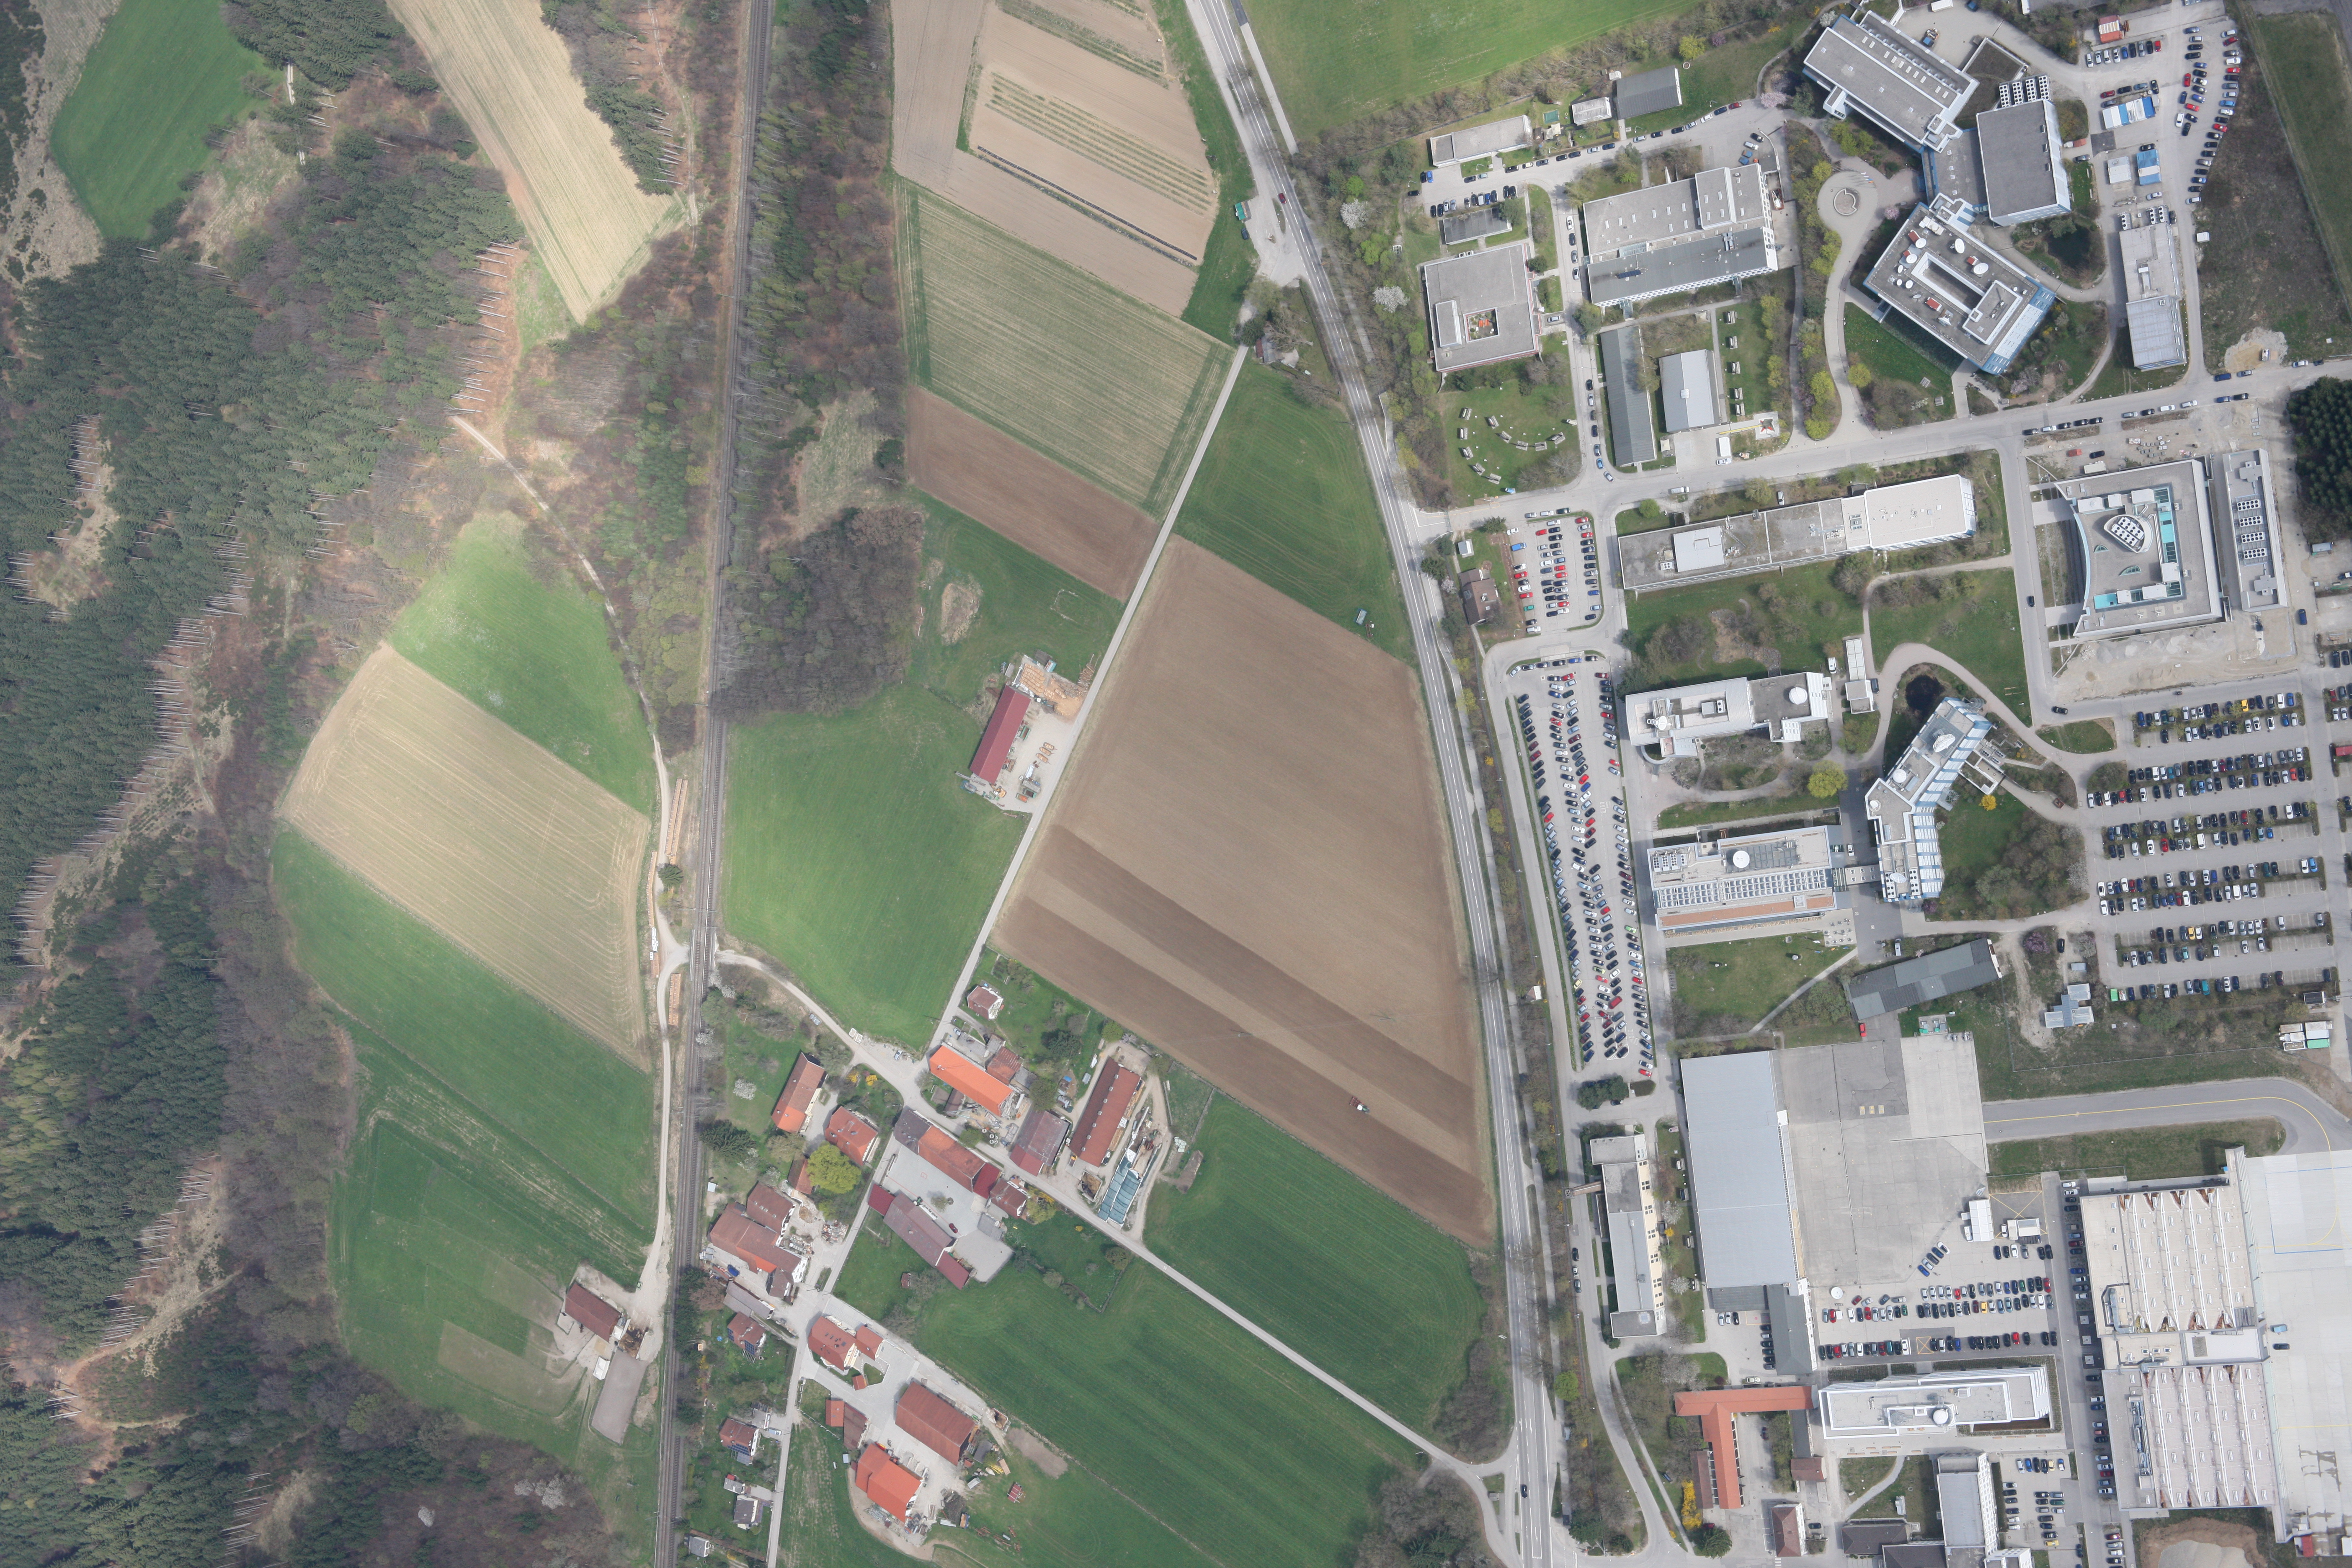
\includegraphics[width=0.5\textwidth]{EK7P0089}};
    \zoombox[magnification=7,color code=yellow]{0.68,0.43}
    \zoombox[magnification=7,color code=red]{0.79,0.44}
    \zoombox[magnification=12,color code=blue]{0.63,0.62}
    \zoombox[magnification=12,color code=green]{0.62,0.7}
\end{tikzpicture} 
 \end{subfigure}

 \begin{subfigure}{0.244\columnwidth}
   \centering
\begin{tikzpicture}
   \centering
    \node[inner sep=0pt] (ima) at (0,0) {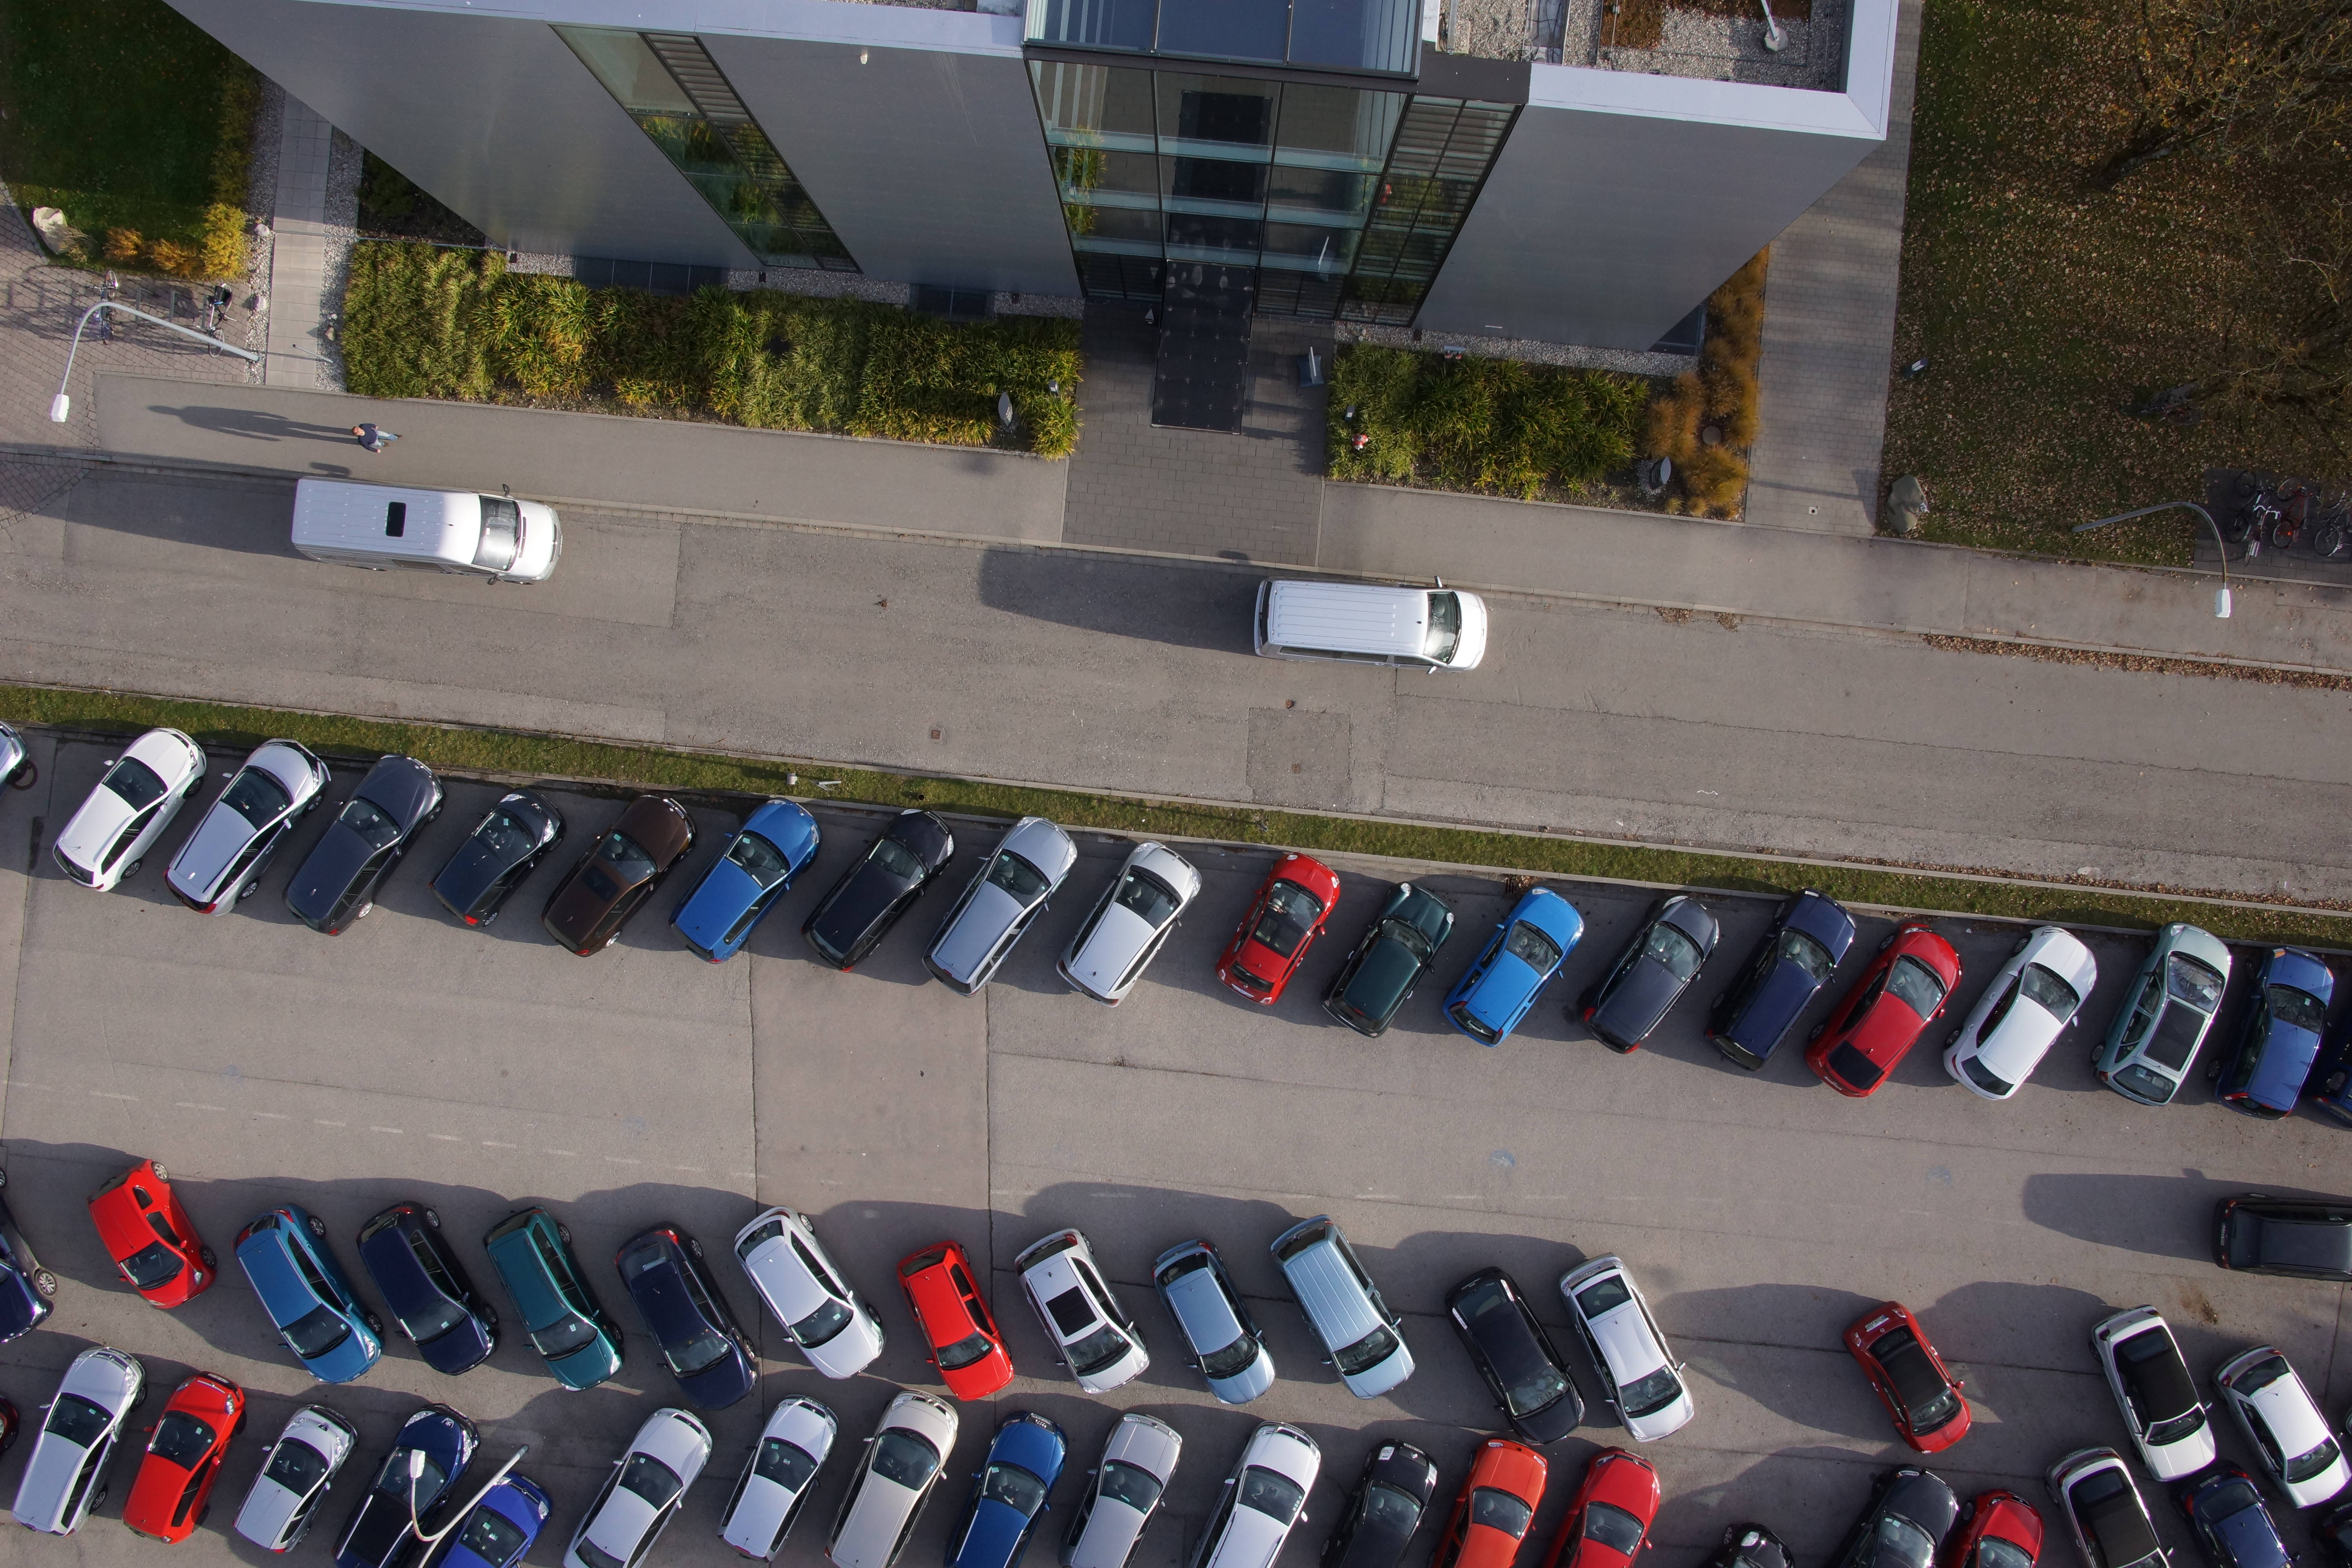
\includegraphics[cfbox=yellow,width=1\columnwidth]{G0000786}};    
 \end{tikzpicture}
 \end{subfigure}
  \begin{subfigure}{0.244\columnwidth}
   \centering
\begin{tikzpicture}
   \centering
    \node[inner sep=0pt] (ima) at (0,0) {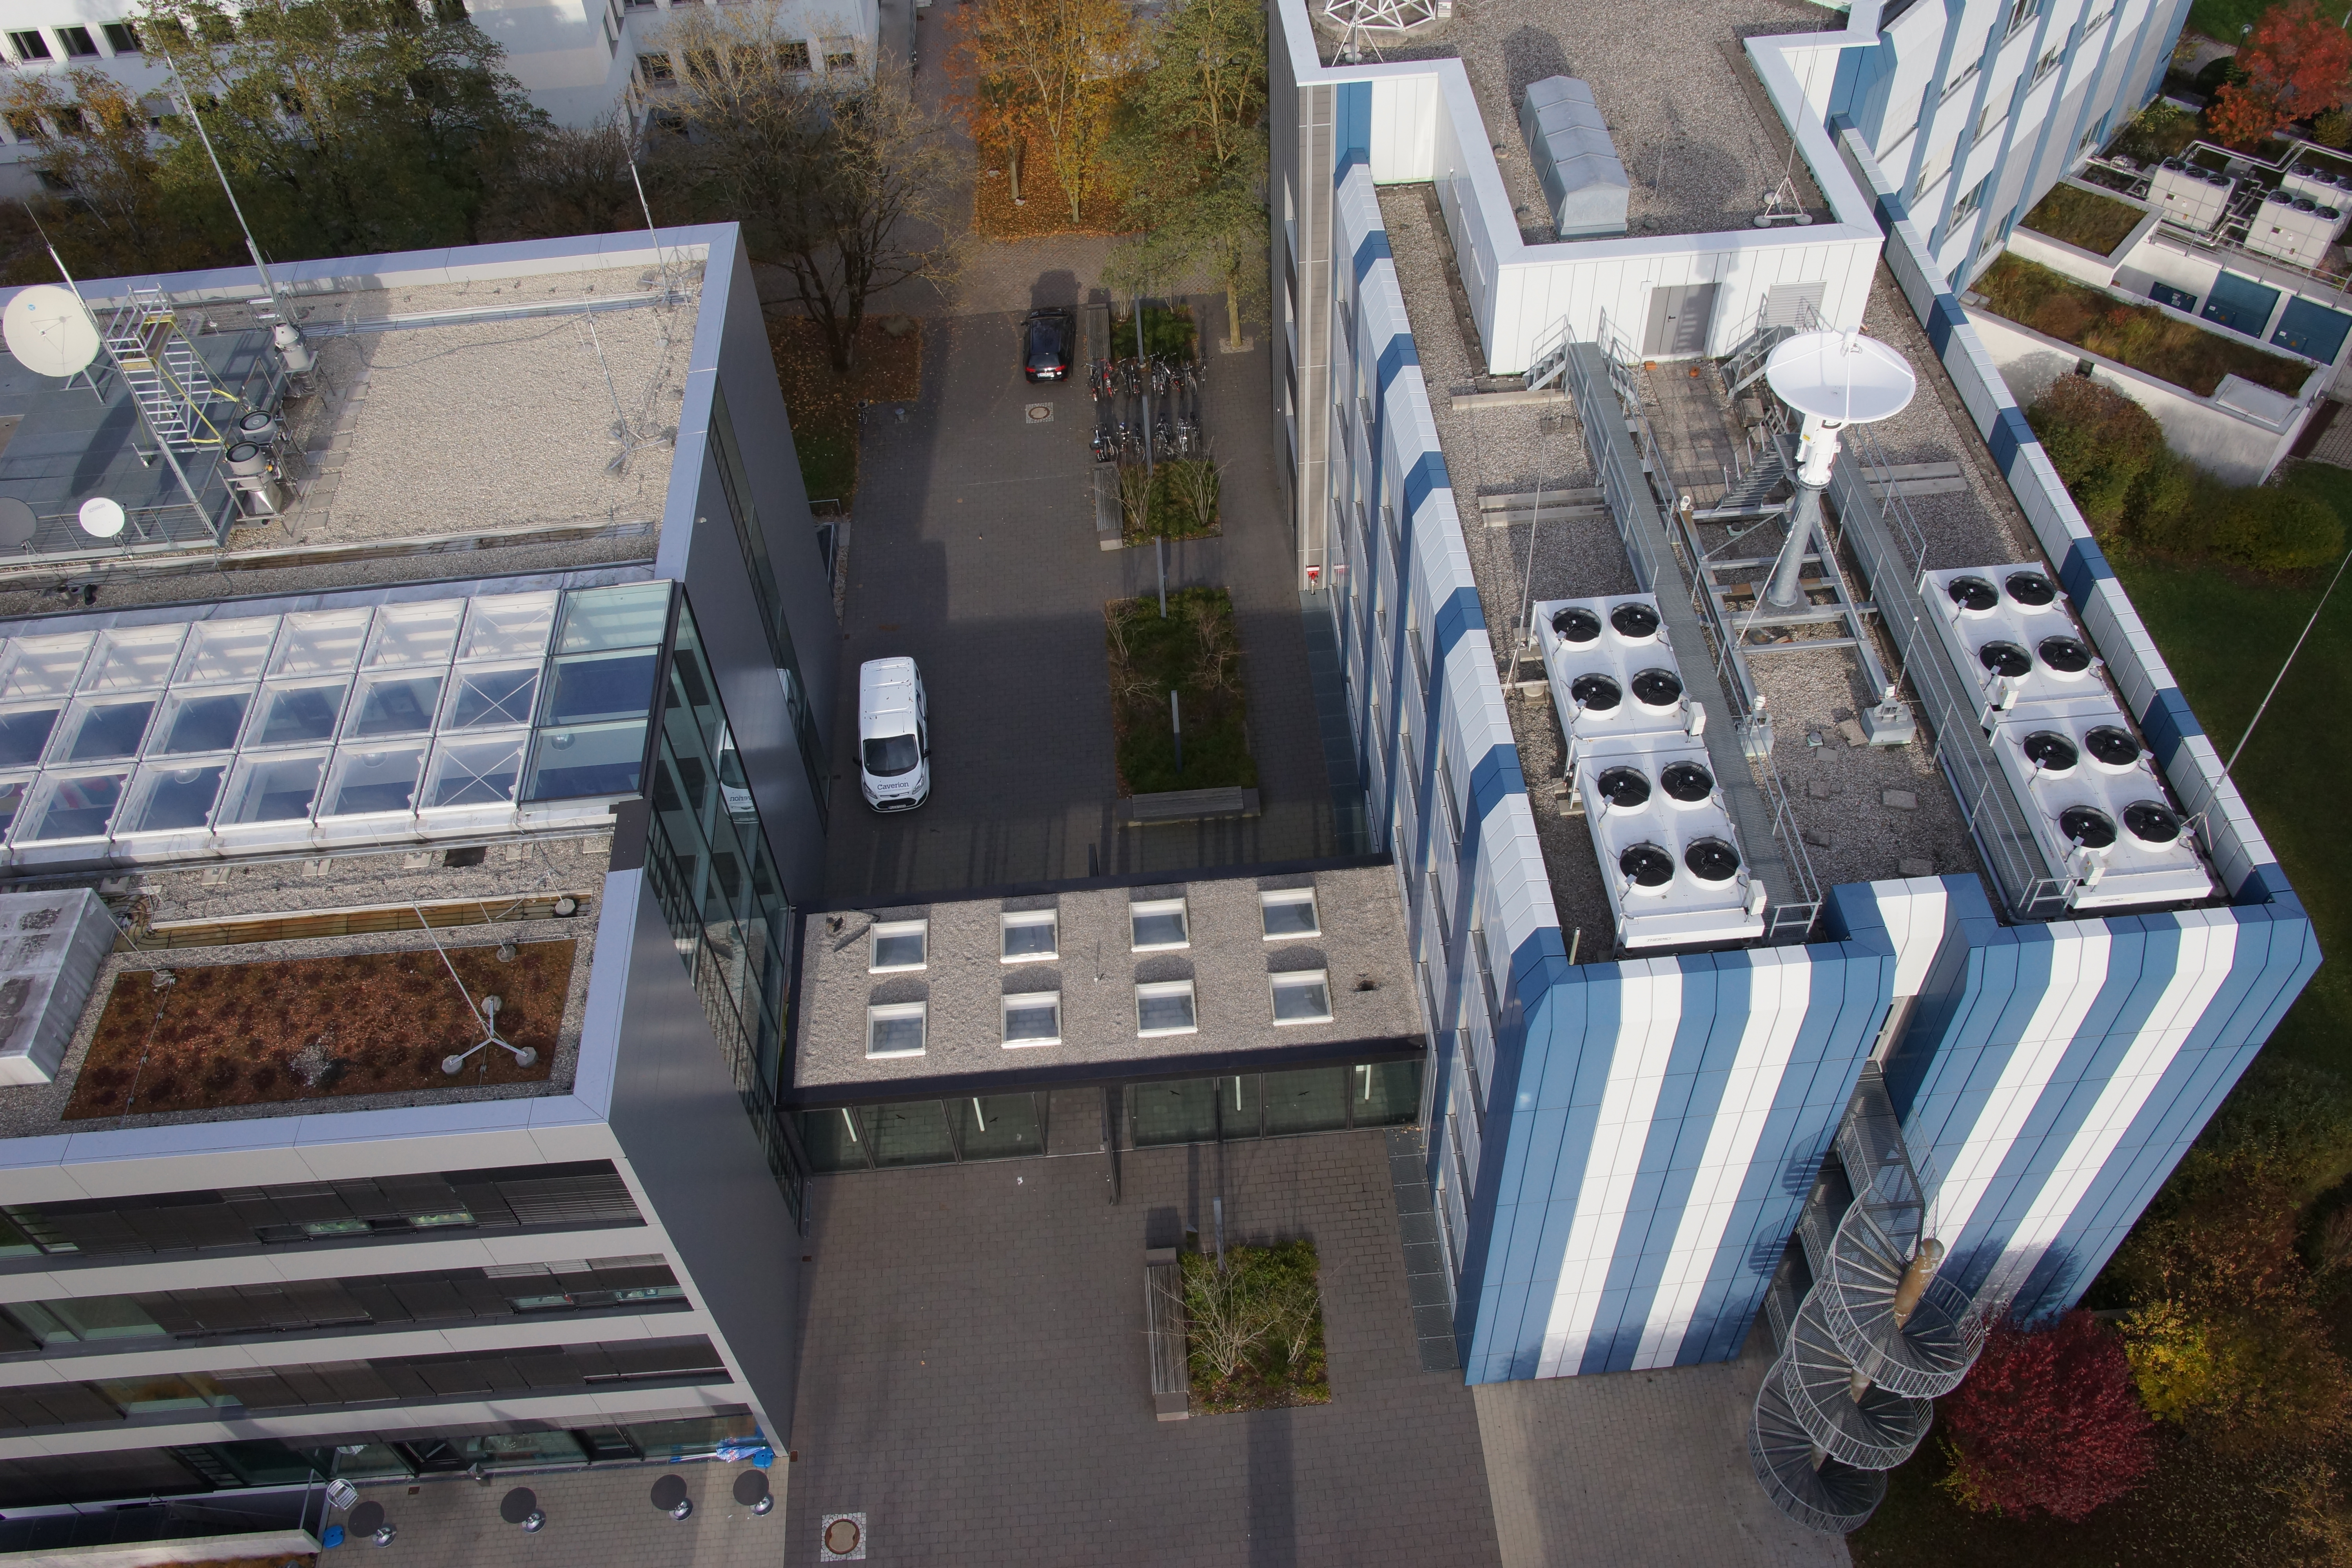
\includegraphics[cfbox=red,width=1\columnwidth]{G0000852}};    
 \end{tikzpicture}
 \end{subfigure}
  \begin{subfigure}{0.244\columnwidth}
   \centering
\begin{tikzpicture}
   \centering
    \node[inner sep=0pt] (ima) at (0,0) {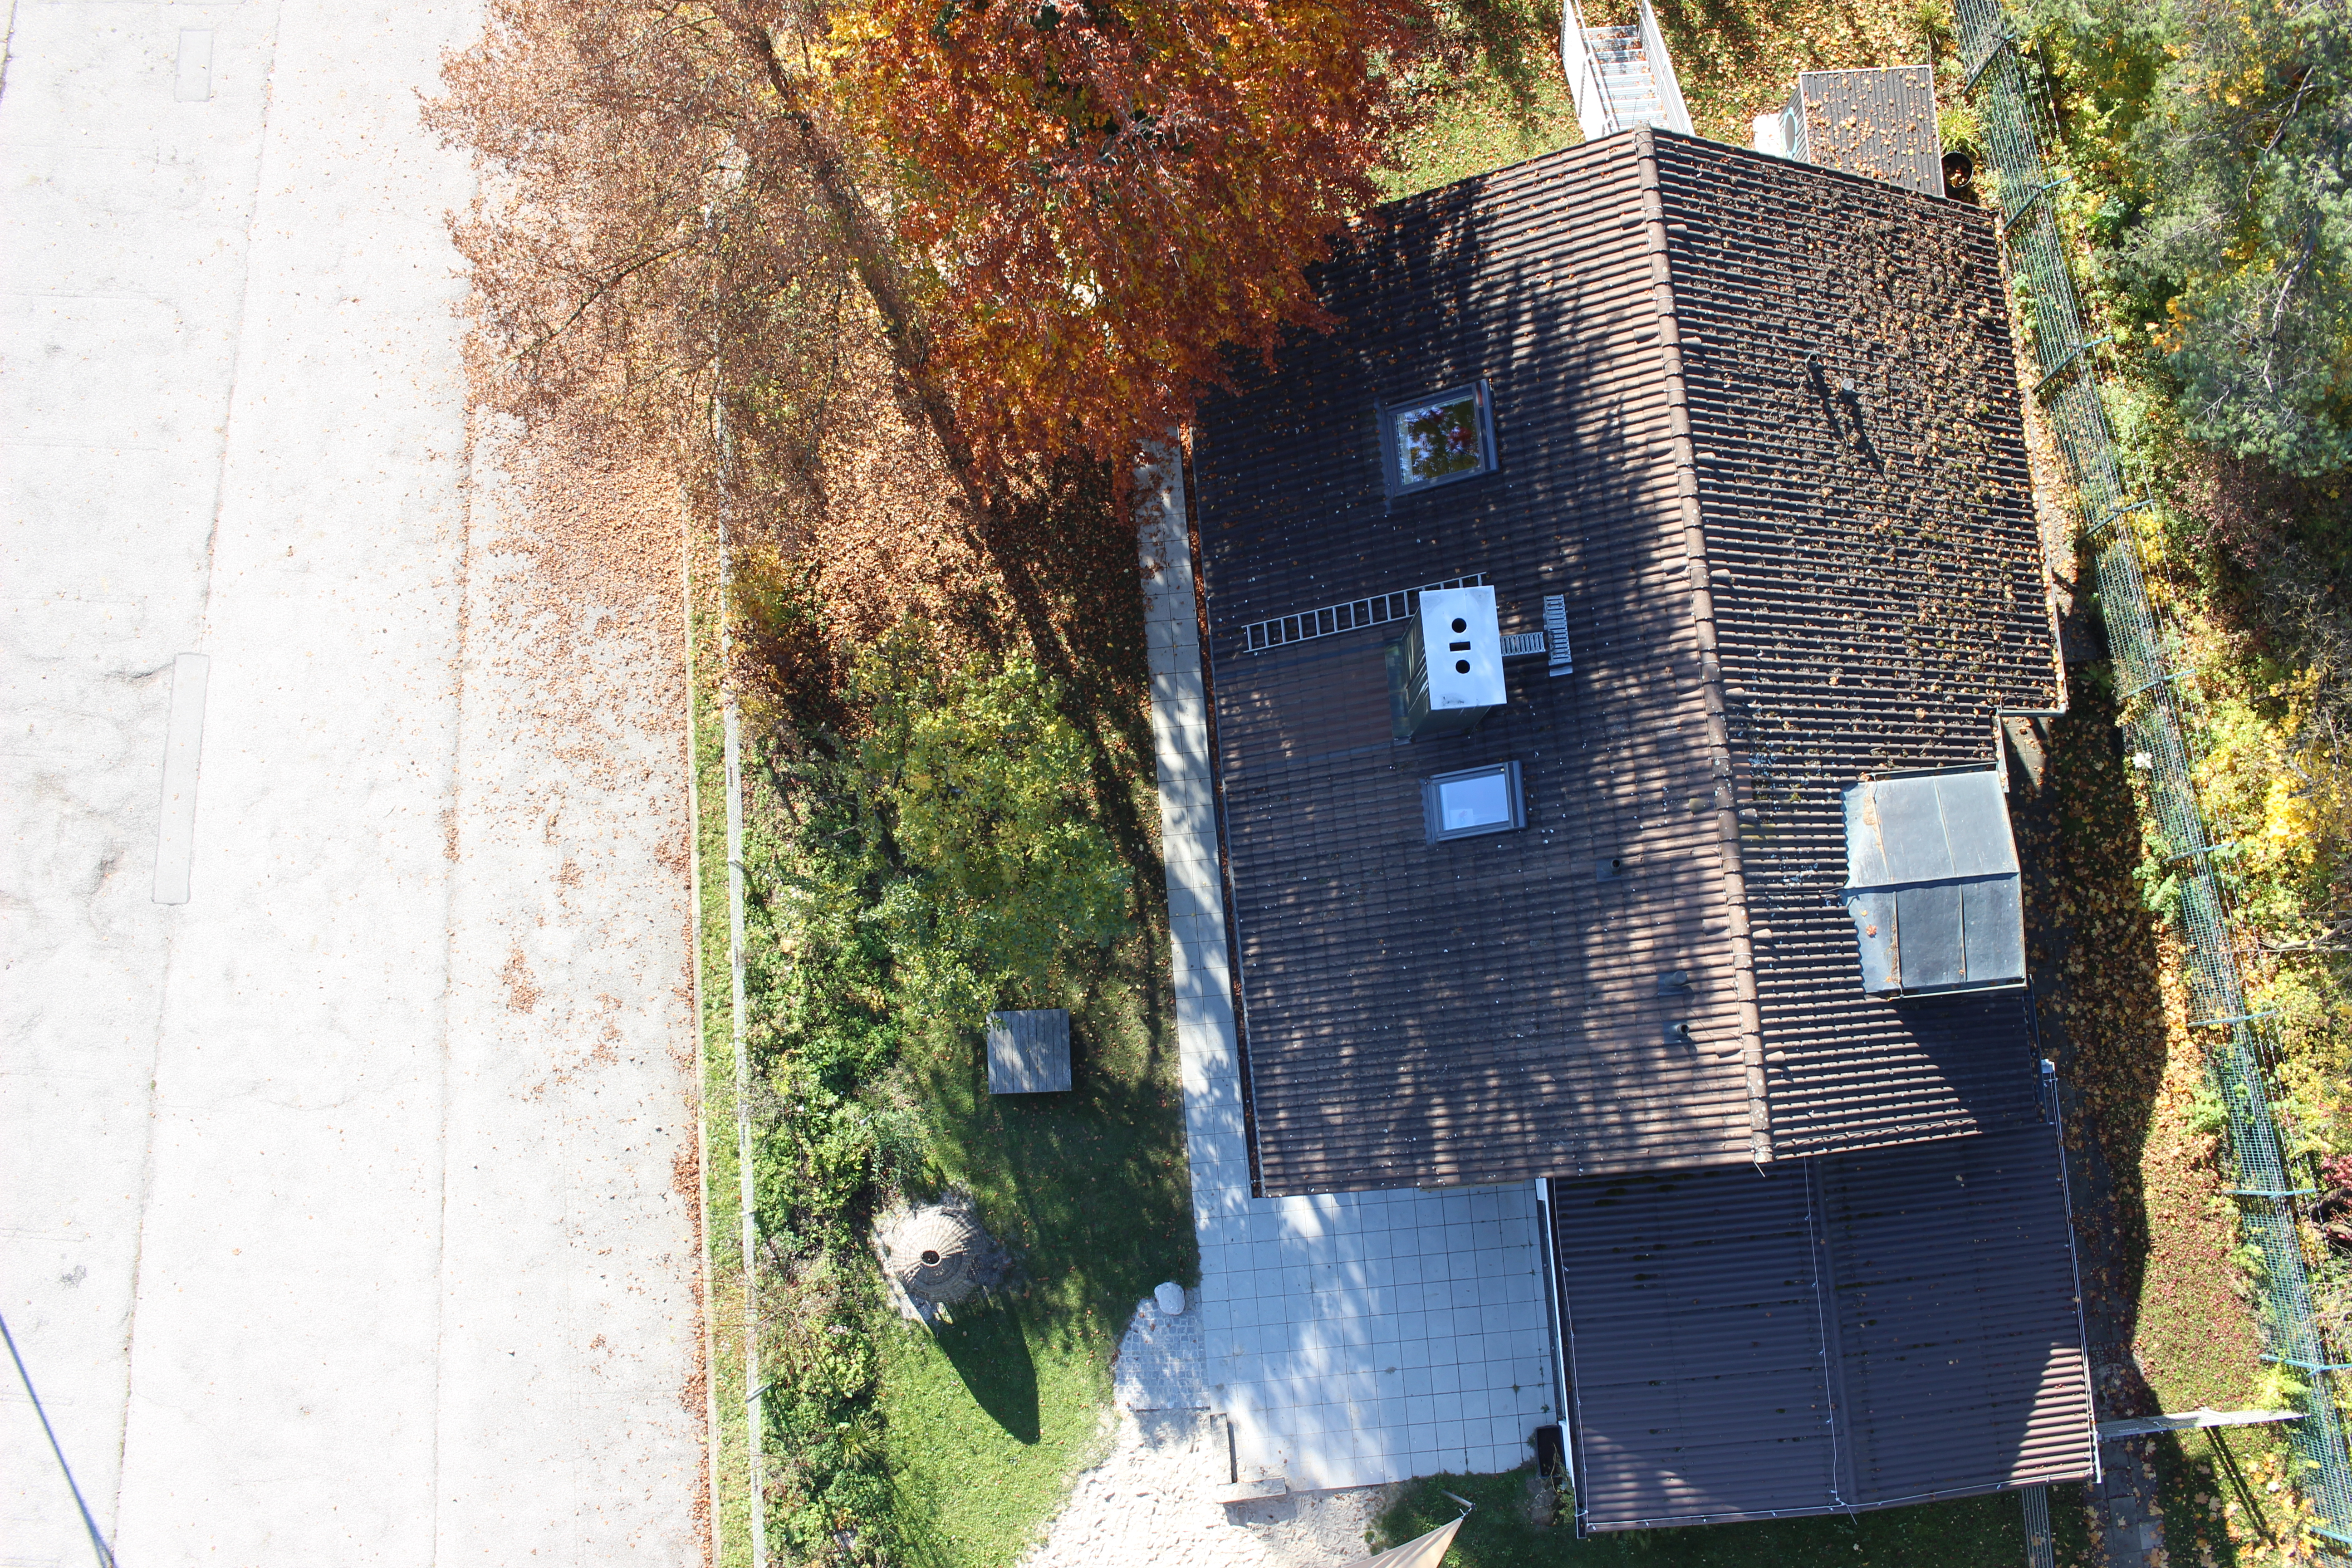
\includegraphics[cfbox=blue,angle=180,width=1\columnwidth]{IMG_1312}};    
 \end{tikzpicture}
 \end{subfigure}
  \begin{subfigure}{0.244\columnwidth}
   \centering
\begin{tikzpicture}
   \centering
    \node[inner sep=0pt] (ima) at (0,0) {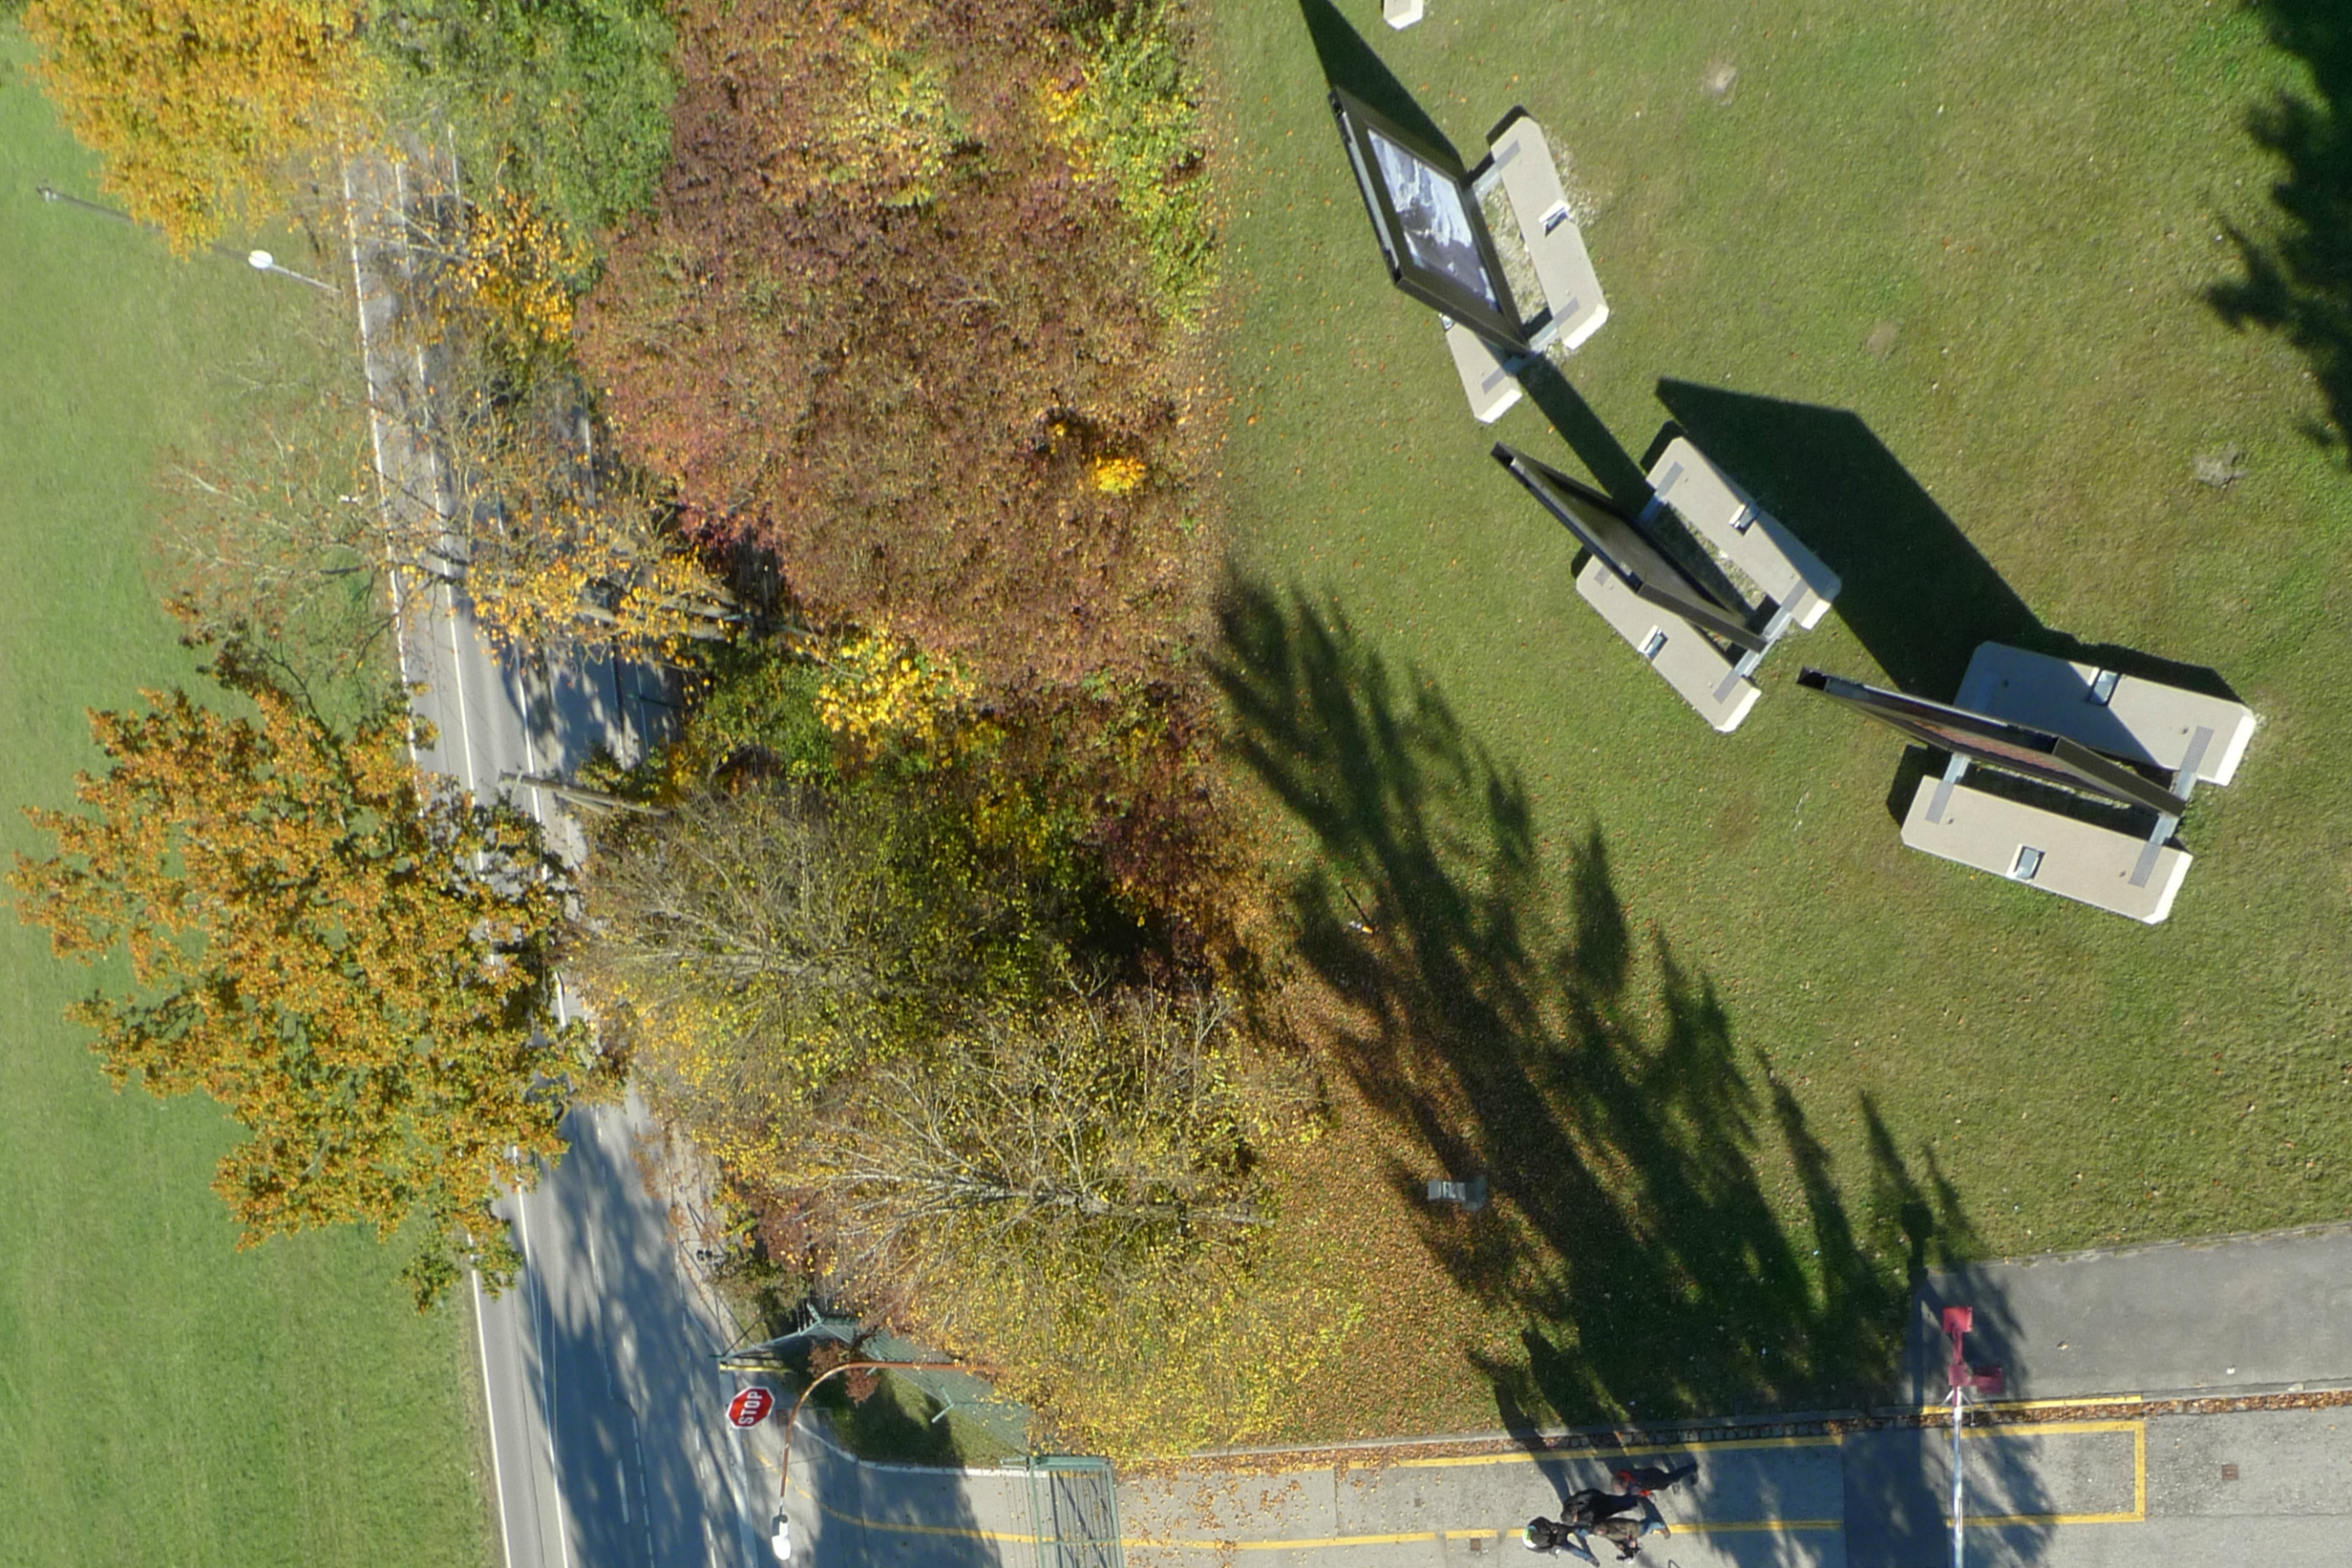
\includegraphics[cfbox=green,width=1\columnwidth]{P1110932}};    
 \end{tikzpicture}
 \end{subfigure}
\vspace{1.1\baselineskip}
\centerline{\textbf{(c)}}
 \caption{Comparison of UAV and aerial imagery. (a) aerial image, (b) magnified areas in aerial image, (c) UAV images featuring corresponding areas}
\end{figure}
 
On the other hand, the coverage of UAV imagery is of limited extent, therefore UAVs are typically used for small-scale mapping as an efficient alternative to full-scale aerial mapping. The total costs of UAV platforms are thus expected to be kept to a minimum, which is usually at the cost of the accuracy of onboard GNSS/IMU systems. Table \ref{tab:comp_acc} compares the accuracy and price of onboard GNSS/IMU systems for UAV and conventional airborne platforms

\begin{table}[H]
  \begin{center}
  %\footnotesize 
  \small
  \begin{tabular}{@{}p{.23\linewidth}p{.25\linewidth}p{.4\linewidth}@{}}
    \toprule
    {} & {\textbf{GNSS/IMU on UAV (NEO-M8)}} & {\textbf{GNSS/IMU on manned aircraft (xOEM)}} \\
    \cmidrule(){1-3}
    % %
    Horizontal accuracy & $2.5$ m & $0.02$ m \\
    \midrule
    Vertical accuracy & $5$ m & $0.03$ m \\
    \midrule
Heading accuracy& $0.3^{\circ}$  & $0.05^{\circ}\sim0.1^{\circ}$\\
    \midrule
    % %
    Price & $30$ \euro{} & $15000$ \euro{}\\ 
    \bottomrule
  \end{tabular}
  \end{center}
  \caption {Comparison of onboard GNSS/IMU systems for UAVs and conventional manned aircrafts}
\label{tab:comp_acc}
\end{table}

Drones are increasingly being used for surveying building construction, road maintenance, and infrastructure inspections. Agricultural applications include crop inspection, and tracking farm animals. 
\include{1_BodyMatter/Review}
\chapter{Automatic UAV Image Geo-Registration by Matching UAV Images to Georeferenced Image Data}
\label{ch:registration}


\newcolumntype{x}{l}
\newcolumntype{X}{>{\footnotesize}l}
\newcolumntype{v}[1]{>{\raggedright\hspace{0pt}}p{#1}}
\newcolumntype{V}[1]{>{\scriptsize\raggedright\hspace{0pt}}p{#1}}





\newcommandx{\note}[2][1=]{\todo[linecolor=red,backgroundcolor=red!25,bordercolor=red,#1]{#2}}


Emerging as novel image acquisition platforms, Unmanned Aerial Vehicles (UAVs) bridge the gap between aerial and terrestrial photogrammetry and offer an alternative to conventional airborne image acquisition systems. 
In comparison to airborne or satellite remote sensing, UAVs stand out for low cost, the utility to be used in hazardous or inaccessible areas and the ability to achieve high spatial and temporal resolutions.
Table \ref{tab:comp_UAV} compares the main features of UAVs and manned aircrafts based on the surveys of \cite{eisenbeiss2009uav} and \cite{nex2014uav}. 
In contrast with manned aircrafts, UAVs have smaller coverage due to lower flight altitude, but they are able to achieve high ground sampling distance (GSD) with lower cost and better flexibility.
While manned aircrafts require big landing fields and pilots, UAVs only need small landing sites and can be remotely controlled, therefore they can work even in hazardous areas and severe weather conditions.
%The joint use of complementary data from different domains can improve the results of various applications, e.g., refining an existing map, precise monitoring, or 3D reconstructions.
Hence, UAVs have been widely involved in remote sensing applications, such as disaster management, urban development, documentation of cultural heritage or agriculture management \cite{colomina2014unmanned}. 


\begin{table}[tbp]
  \begin{center}
  %\footnotesize 
  \small
  \begin{tabular}{@{}p{.29\linewidth}p{.31\linewidth}p{.34\linewidth}@{}}
    \toprule
    {} & {\textbf{UAV Photogrammetry}} & {\textbf{Manned Aircraft Photogrammetry}} \\
    \cmidrule(){1-3}
    Coverage & $m^{2}$ - $km^{2}$ & $km^{2}$ \\
    \addlinespace
    % %
    Image resolution/GSD& $mm - cm$ & $cm-dm$ \\
    \addlinespace
    % %
    Geo-registration possibility &  low quality GNSS/IMU & high quality GNSS/IMU \\
    &meter-level accuracy &centimeter-level accuracy\\
    \addlinespace
    % %
    Price and operating cost&low - moderate&high\\ 
    \addlinespace
    % %
    Flexibility & applicable in hazardous areas & less mobile\\ 
  & works in cloudy/drizzly weather & weather-dependent \\
  & remotely controlled & pilot needed \\
  \bottomrule
  \end{tabular}
  \end{center}
  \caption {Comparison between UAV and manned aircraft photogrammetry}
\label{tab:comp_UAV}
\end{table}


Accurate geo-registration of UAV imagery is a prerequisite for UAV geolocalization and many photogrammetric applications, such as generating georeferenced orthophotos, 3D point clouds or DSMs. 
However, accurate geo-registration of UAV imagery is still an open problem. Limited by on-board payload restrictions, UAVs are equipped with lightweight GNSS/IMU systems, whose georeferencing accuracies are in the range of meters \cite{chiabrando2013direct} and far from the centimeter-level accuracy of airborne photogrammetry \cite{jacobsen2010, Zhao2014122}. 
In order to achieve higher geo-registration accuracy beyond hardware limits, we use a pre-georeferenced aerial or satellite image as a reference, and register the UAV image to the reference image with a novel feature-based image matching method.
%in the coordinate system of the reference dataset by means of bundle block adjustment. 
%The aim is to achieve high accuracy for UAV geo-registration beyond hardware limits.

% \begin{table}[tbp] 
% \begin{center}
% \footnotesize 
%  \begin{tabular}[height=2cm]{|l|l| l|}
%  \hline
%   & UAV photogrammetry &  Manned aircraft photogrammetry\\\hline
%   Coverage& $m^{2}$ - $km^{2}$& $km^{2}$\\\hline
%   Image resolution/GSD& $mm - cm$ & $cm-dm$ \\\hline
%   \multirow{2}{*}{Geo-registration possibility}& low quality GNSS/IMU & high quality GNSS/IM\\
%   &meter-level accuracy &centimeter-level accuracy\\\hline
%   Price and operating cost&low - moderate&high\\\hline
%   \multirow{3}{*}{Flexibility} & applicable in hazardous areas& less mobile\\ 
%   & works in cloudy/drizzly weather & weather-dependent \\
%   & remotely controlled & pilot needed \\ \hline
% \end{tabular}  
% \end{center}
% \caption {Comparison between UAV and manned aircraft photogrammetry}
% \label{tab:comp_UAV}
% \end{table}


In the field of image matching, numerous algorithms for different matching scenarios have been proposed in the last few decades.
%While most of them rely on image pairs from the same domain with low temporal changes of the scene and moderate baselines between the image centers, it is still an open question to match images from multi-platforms, e.g., UAVs, manned aircrafts and satellites.
The biggest challenge for UAV and aerial image matching lies in the substantial differences in their scales, viewing directions and temporal changes. 
For instance, the flight altitude of UAV platforms is about $\SI{50}{\m} - \SI{120}{\m}$ above the earth whereas aerial images are usually captured at $\SI{800}{\m} - \SI{1500}{\m}$ from different viewing directions. 
Although state-of-the-art feature-based image matching methods are generally working fine for many different image pairs and are said to be invariant to changes in viewpoints, wider baselines and local changes of the scene, they surprisingly failed in many of our test cases. 
Figure \ref{fig:failure} illustrates two typical cases of UAV and aerial image matching using SIFT \cite{lowe2004distinctive}.

\begin{figure}[tbp]
    \centering
       \begin{subfigure}[b]{0.47\columnwidth}
           \centering
           \includegraphics[width=\columnwidth]{figures_1/container_sift.JPG}
           \caption[]{\texttt{Container}}%
           {{\small }}
           \label{fig:failure_container}
       \end{subfigure}
       \hfill
       \begin{subfigure}[b]{0.5\columnwidth}  
           \centering 
           \includegraphics[width=\columnwidth]{figures_1/highway_sift.JPG}
           \caption[]{\texttt{Highway}}%
           {{\small }}    
           \label{fig:failure_highway}
       \end{subfigure}
       \caption{Typical cases from the datasets (a) \texttt{Container} and (b) \texttt{Highway} showing the results of matching UAV and aerial images using SIFT, where, left of the subfigure is a downsampled UAV image and right is a cropped aerial image. Green lines indicate the matches detected by SIFT, almost all of them are wrong.}
        \label{fig:failure}
\end{figure}

Even though the scale difference has been eliminated by down sampling the UAV image towards the aerial image and the aerial image has been cropped to the same region as the UAV image, no reliable set of correct matches could be found in the similar looking image pairs. 
This finding motivated us to analyze the reasons for the failure and to develop a new image matching strategy facilitating a successful and robust matching of imagery with wide baselines and substantial geometrical and temporal changes.
%An exhaustive analysis on numerous multi-platform images was carried out using feature-based matching methods to show the problems but also the reasons for the failure. 
%To this end, we propose a novel feature matching method, which can robustly handle the large differences regarding scale and rotation of image pairs. 
%The method is comprised of a dense feature detection scheme, a one-to-many matching strategy and a global geometric constraint for verifying multiple matching hypotheses and delivers thousands of valid matches between UAV and reference imagery whereas standard feature-based matching methods mostly fail. 
%Those abundant and reliable matches contribute to the success of the bundle block adjustment of UAV images. 
%To analyze the accuracy of our matching methods a series of experiments involving different scenarios are conducted.
The obtained 2D matches are used for geo-registration of the UAV image with reference to the aerial image.
%A comparison of triangulated feature points from aerial and UAV images, as well as highly accurate check points  
%An analysis of 3D errors from triangulated points and highly accurate 3D check points of two scenes are computed.
The results demonstrate that our approach achieves decimeter-level co-registration accuracy and comparable absolute geo-registration accuracy as the reference image.

In summary, the main innovations of this paper cover following aspects:
\begin{itemize}[leftmargin=*,labelsep=4mm]
\item An exhaustive analysis of limiting cases of SIFT-based image matching for UAV and aerial image pairs. The reasons for the matching failure are identified by investigating the influence of different SIFT and ASIFT parameters, image rotations and the ratio-test.
\item A novel feature-matching pipeline constituted of a dense feature detection scheme, a one-to-many matching strategy and a global geometric verification scheme.
\item A comprehensive analysis of the matching quality with ground-truth correspondences and a demonstration of various experiments for evaluating absolute and relative accuracies of generated  photogrammetric 3D products.
%\item The robustness of the matching methodology in complicated scenes and accuracy evaluations are showcased. Beside the analysis of the 2D matching quality with ground-truth correspondences, the matches are used for merging UAV and aerial 3D point clouds and for generating georeferenced DEMs. A 3D accuracy evaluation is conducted by comparing 3D point clouds from geo-registered UAV images with georeferenced aerial point clouds and precisely measured ground control points (GCPs).
\end{itemize}

The paper is organized as follows: Section \ref{sec:RelWork} gives a review of related works; Section \ref{sec:Analysis} introduces limiting cases for SIFT matching and outlines the key factors accounting for the failure of the matching. 
Section \ref{sec:method} proposes the novel feature matching method for a robust and reliable matching result for wide-baseline image pairs.
In Section \ref{sec:experiments}, various experiments are carried out to validate the accuracy of the proposed matching method. 
Beside a qualitative and quantitative analysis of the obtained matches of UAV and aerial images, 3D errors of triangulated matches from geo-registered UAV images are compared towards 3D points from aerial imagery and towards terrestrial measured ground control points (GCPs). 
Additionally, DSMs generated from geo-registered UAV images and from aerial images are compared and a joint 3D point cloud is presented.
Finally, Section \ref{sec:disc} discusses the applicability and limitations of the proposed method and Section \ref{sec:conclusion} concludes the paper and describes further applications.

%%%%%%%%%%%%%%%%%%%%%%%%%%%%%%%%%%%%%%%%%%%%%%%%%%%%%%
\section{Related Work}\label{sec:RelWork}
The availability of georeferenced imagery is a prerequisite for many photogrammetric tasks, such as the generation of registered 3D point clouds, DSMs, orthorectification, mosaicking or 3D reconstructions of buildings. 
The key for precise georeferencing of the mentioned products lies in an accurate geo-registration of the captured images, which can be tackled in different ways.
In the field of aerial photogrammetry high-end GNSS/IMU localization sensors are used which allows direct georeferencing of the images without the need of external GCPs or photogrammetric adjustments in a post-processing step. 
Many established systems in aerial photogrammetry have access to such accurate sensors and achieve centimeter-level registration accuracy. 
The relatively low-cost \texttt{DLR 3K} sensor system \cite{kurz2012low} presents a camera frame carried by either a airplane or helicopter and consists of three Canon EOS 1Ds Mark II cameras looking in nadir, forward, and backward direction developed for real time disaster monitoring.
The synchronized image acquisition and localization information provided by the expensive and heavy GNSS/IMU system ($\SI{4}{\kg}$ in total) allows for direct georeferencing accuracies of $\SI{10}{\cm}$ \cite{kurz2014performance}.
The \texttt{Vexcel UltraCam} \cite{ultracam} offers a high level optical sensor for high resolution aerial photogrammetry with more than 100 megapixel. 
Combined with the high-end \texttt{UltraNav}-GNSS/IMU system \cite{ultranav}, $\SI{5}{\cm}$ accuracy for direct georeferencing can be achieved.
Due to payload limitations, many commercial UAVs are usually equipped with lightweight sensors providing localization accuracies in the range of meters \cite{verhoeven2013positioning}, which is not sufficient enough for photogrammetric applications using direct georeferencing. 
%This accuracy level is sufficient for rough geo-registration usable for applications like rapid response or disaster assessment as shown in \cite{nex2014uav} but not applicable if higher georeferencing is needed.
An investigation regarding the ability of direct georeferencing with UAV systems shows that the geolocalization accuracy of current UAV systems is still too low to perform direct applications of photogrammetry at very large scale \cite{chiabrando2013direct}.

For this reason, image-based methods are usually utilized to facilitate geo-registration of UAV imagery in centimeter-level accuracy.
One way to augment geo-registration results is to deploy GCPs, which is even recommended for high-end devices due to the existence of systematic errors \cite{gerke2016accuracy}. 
Nevertheless, the deployment of GCPs is often expensive, requires fieldwork operations and is unpractical or even impossible for hazardous or inaccessible regions. 
Due to the growing accessibility of high resolution aerial and satellite imagery, image matching approaches present a promising alternative for geo-registration. 
Here, geo-registration of UAV imagery is done by matching UAV images with georeferenced databases, such as 3D models, aerial images, orthophotos or satellite images.
An accurate geo-registration of UAV images depends on the accuracy and reliability of the image matching result.
%Numerous matching algorithms contributed to improve this long-standing problem of image matching, but however, there are still many cases where existing methods fail or perform poorly.
Although image matching is a long-standing problem and lots of research has been performed in this area, still many cases exist where established methods fail or perform poorly.
The task of matching UAV and aerial images can be characterized by wide baselines, large differences in viewpoints, and geometrical as well as temporal changes.
Among intensity-based and frequency-based matching methods, local feature-based matching methods perform best with regard to these matching conditions \cite{zitova2003image}.
Among various feature-based matching algorithms, SIFT \cite{lowe2004distinctive} stands out for its robust scale and rotation invariant property. 
Although many variants and alternatives have been developed, such as its approximation SURF \cite{bay2008speeded} and the binary descriptor BRIEF \cite{calonder2010brief}, investigations demonstrate that SIFT is still more robust to viewpoint changes and common image disturbances than both BRIEF and SURF \cite{calonder2012brief}.
ORB \cite{rublee2011orb}, which is a combination of the FAST detector \cite{rosten2010faster} and the BRIEF binary descriptor is a good choice for real-time applications but several evaluations state that it can not reach the repeatability and discriminative properties of SIFT \cite{heinly2012comparative,bekele2013evaluation,dwarakanath2012evaluating,juan2009comparison}.
KAZE \cite{alcantarilla2012kaze} is a new development and succeeds especially in presence of deformable objects. 
As a variant of SIFT, a full affine invariant matching framework ASIFT \cite{yu2011asift} was proposed to handle big differences in viewpoints by simulating a series of transformed images to cover the whole affine space. 
In the case of matching images with large differences in viewpoints, ASIFT has more robust performance than SIFT, which was also confirmed in the evaluation presented in \cite{apollonio2014evaluation}.

Apart from feature-based wide baseline matching, other concepts also investigate different methods for geo-registration of UAV imagery.
Intensity-based methods, like an on-board correlation-based method to register UAV images towards aerial images in case of GNSS outages \cite{conte2009vision} or deformable template matching with image edges and entropy as feature representation \cite{fan2010registration} do usually not perform well in case of temporal and geometrical changes.
More recent work also focus on matching terrestrial and aerial images showing extremely large viewpoints changes.
A new feature representation using a Convolutional Neural Network (CNN) is learned for geolocalizing ground-level images with an aerial reference database \cite{lin2015learning}.
However, manual interventions are needed to estimate the scale for ground-level queries, and the absolute orientation of the query image can hardly be estimated.
Shan et al. \cite{shan2014accurate} synthesizes aerial views from pre-aligned Google Steet View images using depth maps and corresponding camera poses, which are then matched with aerial images using SIFT.
A similar approach is presented by Majdik et al. \cite{majdik2015air}, where UAV images are matched with geo-tagged street view images using ASIFT achieving meter-level global accuracy.
However, only low altitudes and oblique images facing building fa\c{c}ades are considered for the geo-registration.
Aicardi et al. \cite{aicardi2016image} adopts an image-based approach for co-registering multi-temporal UAV image datasets, however, it only estimates the relative transformation between the epochs, while the absolute transformation of the epoch is not solved.
Finally, Xu et al. \cite{xu2016mosaicking} presents an fast and efficient way for UAV image mosaicking without the explicit computation of camera poses, however the image mosaics are not geo-registered.


Although considerable attempts and progress have been made regarding this topic, many of them rely on intensity-based matching methods, which are proven to be unstable in case of geometric or temporal changes. 
In this sense, robust image matching against large scale and viewpoint differences is the key to solve the problem for which feature-based approaches are still the methods of choice.
Some mentioned approaches focus on improving the matching result for extremely large viewpoint changes, but still do not reach the desired global georeferencing accuracy.

% In addition, the accuracy of those image-based methods is limited by the performance of image matching. 
% Despite the fact that some methods apply geometric constraints to improve the matching accuracy, they still have difficulty in matching images with large differences in scales and viewpoints. 

Our approach is based on previous work \cite{koch2016new,zhuo2016fusion}, which have been proven to work for complex matching scenarios with multi-scale images. 
Compared with the state-of-the-art works mentioned above, our method is an advancement in following aspects:
\begin{itemize}[leftmargin=*,labelsep=4mm]
%\item Our method does not need GNSS/IMU data to estimate the scale and orientation for image pre-alignment, which enables UAV global registration even in GNSS-denied environments.
\item To handle the large differences in scale and rotation between image pairs, we use a novel feature-matching approach which can overcome the challenge and robustly deliver abundant matches.
\item Our method works for data of different scales, e.g., aerial images, aerial orthophotos and satellite images.
\item Our method achieves not only decimeter-level co-registration accuracy, but also comparable absolute accuracy as that of the reference image, which are georeferenced in the conventional photogrammetric way.
\end{itemize}


% \cite{kaminsky2009alignment} aligned a point cloud reconstructed from SfM with overhead images (e.g. satellite maps floor plans) by projecting the point cloud onto a ground plane and then matching image edges with the overhead image. 
% The drawback is that GNSS information is needed to estimate the position and image edge matching does not work well if the scene is rich in texture. 



%BRISK \cite{leutenegger2011brisk}, , 

%most of them dealing with the reduction of computational time by approximations in specific implementations details, but rarely outperformed SIFT \cite{miksik2012evaluation,juan2009comparison}.
%As a variant of SIFT, a full affine invariant matching framework ASIFT \cite{yu2011asift,morel2009asift} was proposed against the big differences in viewpoints by simulating a series of transformed images to cover the whole affine space. 
%In the case of matching images with large differences in viewpoints, ASIFT has more robust performance than SIFT. 





%Due to the lower performance of the on-board localization sensors , direct georeferencing of UAV imagery is not suitable for many remote sensing applications which require higher positioning accuracy. 
% %Many attempts have been made to solve the problem of UAV global georegistration. 
% %On-board GNSS/IMU data is usually used for direct-georeferencing with accuracies of a few meters \cite{verhoeven2013positioning}. 
% %This accuracy level is sufficient for rough georegistration and therefore widely used for applications like rapid response or disaster assessment \cite{nex2014uav}. 



% The precision of UAV geo-registration is mainly limited by the performance of the on-board hardware.
% While aerial photogrammetry generally has access to high-end GNSS/IMU localization sensors to achieve cm geo-registration accuracy[?],  accurate geo-registration of UAVs is more challenging.
% Due to the lower performance of the on-board localization sensors, direct georeferencing of UAV imagery is not suitable for many remote sensing applications which require higher positioning accuracy. 
% %UAVs are usually equipped with lightweight sensors with accuracies up to few meters \cite{verhoeven2013positioning} and therefore do not provide satisfactorily registration accuracy for many remote sensing applications and direct georeferencing.

% %Many attempts have been made to solve the problem of UAV global georegistration. 
% %On-board GNSS/IMU data is usually used for direct-georeferencing with accuracies of a few meters \cite{verhoeven2013positioning}. 
% %
% For this reason it is generally advised to deploy Ground Control Points (GCPs) even for high-end devices \cite{gerke2016accuracy} due to the existence of systematic errors. 
% Nevertheless, the deployment of GCPs is often expensive, requires high human interaction and is unpractical for hazardous or inaccessible regions. 
% On the other hand, image-based approaches gained a lot of interest due to the growing accessibility of high resolution aerial and satellite imagery.
% Geo-registration of UAV imagery is done by matching UAV images with a georeferenced database, such as 3D models, aerial images, orthophotos, satellite images or Google Street-View images.
% These promising approaches stand out for an automatic and precise geo-registration ability with comparable accuracies to GCPs if the matching process can be done robustly and exactly.

% %Recently, many studies attempted to adopt image-based approaches for UAV georegistration, i.e., to geolocalize the images by matching the images with a georeferenced database, such as 3D models, aerial images, colored orthophotos, satellite images or Google Street-View images.
% %Image-based georegistration approaches benefit from the growing accessibility of high resolution aerial and satellite imagery and stand out for an automatic and accurate georegistration ability if the matching process can be done robustly and precisely.
% % 
% Current matching algorithms can be generally divided into three categories: pixel value-based methods, e.g., Normalized-Cross-Correlation (NCC), which are vulnerable to image intensity changes and geometric deformations [?]; frequency domain-based methods, e.g., wavelet transform-based methods, which are sensitive to local distortions \cite{chen2013invariant}; local feature-based methods, which outperform the other two methods in the mentioned aspects and hence are widely used for matching images with different viewpoints, resolutions and orientations \cite{zitova2003image}. 


% SIFT and ASIFT are scale and rotation invariant in most cases, however, when it comes to the matching of UAV images and aerial images, which have large differences in scales and viewpoints, SIFT and ASIFT turn out to be unreliable and not robust enough. 
% Even after eliminating the differences by downsampling and aligning the images, SIFT and ASIFT still fail. 
% It was pointed out in \cite{sur2011image} that the ratio-test of SIFT \cite{lowe2004distinctive} is likely to discard correct matches when repeated patterns exist.

% Although considerable attempts and progress have been made regarding this topic, they all require GNSS/IMU information for initial image alignment. 
% In addition, the accuracy of those image-based methods is limited by the performance of image matching. 
% Despite the fact that some methods apply geometric constraints to improve the matching accuracy, they still have difficulty in matching images with large differences in scales and viewpoints. 
% In this sense, robust image matching against large scale and viewpoint differences is the key to solving the problem.



% Our approach is based on previous work of \cite{koch2016new} and \cite{zhuo2016fusion}, which have been proven to work for complex matching scenarios with multi-scale images. 
% Compared with the state-of-the-art works mentioned above, our method is an advancement in following aspects:
% \begin{itemize}[leftmargin=*,labelsep=4mm]
% \item Our method does not need GNSS/IMU data to estimate the scale and orientation for image pre-alignment, which enables UAV global registration even in GNSS-denied environments.
% \item Against the large differences in scale and rotation between image pairs, we use a novel feature-matching approach which can overcome the challenge and robustly deliver abundant matches.
% \item Our method works for data of different scales, e.g., aerial images, aerial orthophotos and satellite images.
% \item Our method achieves not only decimeter-level co-registration accuracy, but also comparable absolute accuracy as that of the reference image, which are georeferenced in the conventional photogrammetry way.
% \end{itemize}

%%%%%%%%%%%%%%%%%%%%%%%%%%%%%%%%%%%%%%%%%%%%%%%%%%%%%%%%%%%%%%%%%%%%%%%%%%%
\section{Matching Performance Evaluation Using SIFT Features}\label{sec:Analysis}
This section introduces different UAV and aerial image pairs and a comprehensive analysis of the matching performance using SIFT and ASIFT. 
Although one would expect that SIFT matching can successfully match the presented images, a robust and successful matching is not possible.
In order to figure out why the popular SIFT matching method surprisingly fails, we analyze the influence of different SIFT parameters, such as octaves and levels, the ratio-test, but also image rotations. 
Experimental results demonstrate that the rotation invariance of SIFT is not as good as it has been considered to be and the deficiency in the rotation estimation of SIFT leads to non-optimal matching results. 
In addition to that, many correct matches are either not nearest neighbors in feature space or are rejected after applying the ratio-test.
%Based on this conclusion, we propose a new strategy for matching aerial images and UAV images, and compare the performance of the proposed method with SIFT and ASIFT approaches on different datasets.
%For the experiments we use the SIFT implementation in OpenCV 3.0.

\subsection{SIFT}\label{sec:SIFT}
%Unlike matching images from the same domain, e.g., two aerial or two UAV images, matching between UAV and aerial images (typical altitudes are $\SI{50}{\m} - \SI{120}{\m}$ and $\SI{800}{\m} - \SI{1500}{\m}$ respectively) is more complicated and challenging due to the substantial $5-15\times$ scale difference. 
%With the help of preliminary knowledge from GNSS data, in general the scale difference can be estimated and mostly eliminated by down sampling the UAV image. 

% To extract sufficient and reliable image correspondences is crucial for subsequent image matching and orientation.  
% A popular workflow works as follows \cite{sur2011image}:
% \begin{enumerate}[leftmargin=*,labelsep=3mm]
% \item Detect interest points in both images and compute the descriptors based on local photometry.
% \item Match the interest points according to the similarity of descriptors.
% \item Remove the mis-matches (outliers) by finding a subset of correspondences which are in accordance with the underlying epipolar geometry, e.g. fundamental matrix.
% \item Determine further correspondences using guided matching, i.e., find more putative correspondences by relaxing step 2, and then prune the correspondences based on the estimated geometric constraint in step 3.  
% \item Prune the final set of image correspondences like in step 3.
% \end{enumerate}

%According to various evaluations \cite{heinly2012comparative,bekele2013evaluation,dwarakanath2012evaluating,juan2009comparison}, SIFT has been proven to be more robust and stable than its variants like SURF and ORB and is therefor chosen for a comprehensive analysis of the matching of difficult image pairs.

%In step 1, 
Among the state-of-the-art matching algorithms, SIFT has been proven to be scale and rotation invariant and outperform other local descriptors in various  evaluations \cite{heinly2012comparative,bekele2013evaluation,dwarakanath2012evaluating,juan2009comparison}. Besides, the ratio-test proposed by Lowe \cite{lowe2004distinctive} is widely applied to discard mismatches. 
In view of the substantial differences in scale and rotation of the UAV image and the aerial image, it makes sense to implement the SIFT matching algorithm (we use the OpenCV 3.0 implementation).
This matching method is noted as "standard SIFT" in the following text.

%In the context of matching images with repetitive structures, Step 2 is critical as presented in \cite{sur2011image} and \cite{mok2011serp}. 
% Since the global threshold on the euclidean distance between descriptors in step 2 does not perform well \cite{lowe2004distinctive}, 
% the ratio-test proposed by Lowe is widely applied to discard mismatches by rejecting all potential matches with similar descriptors, i.e., to impose that the ratio of the distances to the first and the second nearest neighbor is smaller than a certain threshold. 
The ratio-test discards mismatches by rejecting all potential matches with similar descriptors. It works well in most cases, however, applying the ratio-test in feature-based matching methods for images with repetitive structures often causes problems with similar descriptors. 
In this case, the distance ratio can be so high that these features would probably be defined as outliers.
This can be critical especially when only a few correspondences remain after matching.
To investigate how many correct matches are actually discarded by the ratio-test, we implemented SIFT matching and counted the correct matches before and after the ratio-test.
Particularly, the distances of first two nearest neighbors are computed and compared with the threshold. 
Considering that the number of matches can be numerous and it is unrealistic to check every single match manually, we therefore computed the fundamental matrix between the two images with dozens of manually selected image correspondences, and then apply the epipolar constraint using the derived fundamental matrix to filter the raw matches. 
Afterwards, the filtered matches are again checked by manual inspection to ensure the purity of correct matches.

It needs to be pointed out that only a manually cropped part of the aerial image with almost the same image content of the UAV image was used for interest point detection, otherwise SIFT would fail to find correct matches for any dataset.
This simplification of the matching problem is not feasible in practice and is only used for this analysis.
The proposed method is able to match the original uncropped image pairs as this will be discussed in Section \ref{sec:experiments}.

To ensure the best matching result using the SIFT detector and descriptor we comprehensively tested different parameters. 
Specifically, we analyzed the effect of different ratio-test thresholds and different parameters of the SIFT detection, like the number of octaves and levels per octave. 
Other parameters were kept constant as they have only minor effect on the matching result. 
Concretely, we set the contrast threshold to $0.04$, the edge threshold to $10$ and the sigma of the Gaussian to $1.6$. 
An extensive analysis was carried out for all of the datasets in Figure \ref{fig:datasets}, while only the results of the \texttt{Container} dataset is depicted.
Nevertheless, we found similar results for all of our image pairs. 

\begin{figure}[tbp]
    \centering
       \begin{subfigure}[b]{0.243\textwidth}
           \centering
           %\caption{Rural}
           \includegraphics[width=\textwidth]{figures_dataset/container_org_air.jpg}
       \end{subfigure}
       \hfill
       \begin{subfigure}[b]{0.243\textwidth}  
           \centering 
           %\caption{Urban1}
           \includegraphics[width=\textwidth]{figures_dataset/eichenau_org_air.jpg}
       \end{subfigure}
       \hfill
       \begin{subfigure}[b]{0.243\textwidth}  
           \centering 
           %\caption{Pool}
           \includegraphics[width=\textwidth]{figures_dataset/swimmingpool_org_air.jpg}
       \end{subfigure}
       \hfill
       \begin{subfigure}[b]{0.243\textwidth}   
           \centering 
           %\caption{Building}
           %\includegraphics[width=\textwidth]{figures_dataset/eoc_new_org_air.JPG}
           \includegraphics[width=\textwidth]{figures_dataset/eoc_org_4k_air.jpg}
       \end{subfigure}
        \vskip\baselineskip
       \begin{subfigure}[b]{0.243\textwidth}   
           \centering 
           \includegraphics[width=\textwidth]{figures_dataset/container_org_uav.jpg}
           \caption{\texttt{Container}}
       \end{subfigure}
       \hfill
       \begin{subfigure}[b]{0.243\textwidth}  
           \centering 
           \includegraphics[width=\textwidth]{figures_dataset/eichenau_org_uav.jpg}
           \caption{\texttt{Urban1}}
       \end{subfigure}
       \hfill
       \begin{subfigure}[b]{0.243\textwidth}   
           \centering 
           \includegraphics[width=\textwidth]{figures_dataset/swimmingpool_org_uav.jpg}
           \caption{\texttt{Pool1}}
       \end{subfigure}
       \hfill
       \begin{subfigure}[b]{0.243\textwidth}   
           \centering 
           %\includegraphics[width=\textwidth]{figures_dataset/eoc_new_org_uav.JPG}
           \includegraphics[width=\textwidth]{figures_dataset/eoc_new_org_air.JPG}
           \caption{\texttt{Building}}
       \end{subfigure}
       %\vskip\baselineskip
       \begin{subfigure}[b]{0.243\textwidth}  
           \centering 
           \includegraphics[width=\textwidth]{figures_dataset/highway_org_uav.jpg}
           \caption{\texttt{Highway}}
       \end{subfigure}
       \hfill
       \begin{subfigure}[b]{0.243\textwidth}   
           \centering 
           \includegraphics[width=\textwidth]{figures_dataset/eichenau_org_uav2.jpg}
           \caption{\texttt{Urban2}}
       \end{subfigure}
       \hfill
       \begin{subfigure}[b]{0.243\textwidth}   
           \centering 
           \includegraphics[width=\textwidth]{figures_dataset/swimmingpool_org_uav2.jpg}
           \caption{\texttt{Pool2}}
       \end{subfigure}
       \hfill
       \begin{subfigure}[b]{0.243\textwidth}  
           \centering 
           \includegraphics[width=\textwidth]{figures_dataset/eoc_org_gmaps.jpg}
           \caption{\texttt{Googlemaps}}
       \end{subfigure}
       \caption{Datasets used in this paper: Each column represents one (pre-processed) aerial reference image and two UAV target images. The UAV image in (d) should be matched to the aerial image (top right) and to a cropped part of a googlemaps image (h).}
\label{fig:datasets} 
\end{figure}
In a first step of our analysis, we study the effect of different numbers of octaves and levels in the SIFT detection step, while fixing the ratio-test threshold to a commonly used value of $0.75$.
The number of octaves is related to different image samplings, while the number of levels represent the number of scale spaces per octave and is therefore related to the amount of image blurring.
Table \ref{tab:Octaves} lists the number of feasible correct matches from the set of remaining matches after applying the ratio-test for different values of octaves and levels. 
Due to the low image resolutions of the downsampled UAV image ($664 \times 885$ pix) and cropped aerial image ($971 \times 665$ pix), the number of keypoint detections saturates after two octaves. 
While increasing the number of levels per octave results in more matches surviving the ratio-test, the number of inliers stays constant at a very low number of around 20 matches.


\begin{table}[tbp]
\centering
\small 
\begin{tabular}{rlllllllll}
\toprule
\multicolumn{1}{r}{}    &   & \multicolumn{8}{l}{\textbf{Levels}}  \\
\multicolumn{1}{l}{}    &   & \textbf{1} & \textbf{2} &  \textbf{3} &  \textbf{4} & \textbf{5} &  \textbf{6} &  \textbf{7} &  \textbf{8} \\
\cmidrule(lr){3-10} 
\footnotesize
\multirow{5}{*}{\rotatebox[origin=c]{90}{\small \textbf{Octaves}}} & \small \textbf{1} & 12 / 50  & 15 / 61  & 15 / 64  & 17 / 74  & 17 / 84  & 11 / 91  & 17 / 78  & 14 / 91  \\
& \small \textbf{2} & 13 / 61  & 17 / 71  & 12 / 89  & 20 / 103  & 25 / 124 & 16 / 134  & 26 / 137 & 21 / 148  \\
& \small \textbf{3} & 13 / 63  & 17 / 76  & 13 / 93  & 22 / 108  & 26 / 131 & 17 / 142  & 27 / 148 & 22 / 153  \\
& \small \textbf{4} & 13 / 62  & 17 / 77  & 13 / 94  & 22 / 109  & 26 / 134 & 17 / 146  & 27 / 155 & 22 / 158  \\
& \small \textbf{5} & 13 / 62  & 17 / 77  & 13 / 93  & 22 / 110  & 26 / 136 & 17 / 148  & 27 / 157 & 22 / 159  \\
\bottomrule
\end{tabular}
\caption{Analysis of SIFT performance with different octaves and levels for the \texttt{Container} dataset. Cells contain the number of correct matches (first number) from the set of remaining matches (second number) after applying the ratio-test with a fixed threshold of $0.75$. Due to the scale adaption of the UAV image the number of keypoint detections saturates after two octaves. By increasing the levels more keypoints can be detected but the ratio of inliers decreases.}
\label{tab:Octaves}
\end{table}

According to this experimental result, we analyze different thresholds of the ratio-test in a next step while limiting the SIFT detector to three octaves and five levels.
Like in the analysis above, we again count the number of remaining matches after the ratio-test and the number of inliers among them, as illustrated in Figure \ref{fig:Ratio}(a).
A maximum number of around $100$ correct matches can be found when only the first nearest neighbor is considered (equivalent to a threshold of $1$). 
Comparing this number to the total number of around $4000$ matches this is a very low ratio of inliers as can also be seen in Figure \ref{fig:Ratio}(b). 
Increasing the impact of the ratio-test (equivalent to lower values of the threshold), a lot of correct matches are rejected due to a high similarity to other keypoint descriptors, while the ratio of outliers is decreasing at the same time.

According to the results in Figure \ref{fig:Ratio}(b), the best ratio of inliers is suggested for threshold values between $0.3$ and $0.5$, but the absolute numbers of correct matches for these values is below ten and therefore not a reliable matching result.
\begin{figure}[tbp]
    %\centering
       \begin{subfigure}[c]{0.3\linewidth}
	       \centering
			% This file was created by matlab2tikz.
%
%The latest updates can be retrieved from
%  http://www.mathworks.com/matlabcentral/fileexchange/22022-matlab2tikz-matlab2tikz
%where you can also make suggestions and rate matlab2tikz.
%
\definecolor{mycolor1}{rgb}{0.00000,0.44700,0.74100}%
\definecolor{mycolor2}{rgb}{0.85000,0.32500,0.09800}%
%
\begin{tikzpicture}

\begin{axis}[%
width=.9\linewidth,
height=.2\textheight,
scale only axis,
grid = major,
xmin=0,
xmax=1,
tick label style={font=\small},
xlabel style={font=\color{white!15!black}, font=\small},
xlabel={Ratio-test threshold},
%separate axis lines,
every outer y axis line/.append style={mycolor1},
every y tick label/.append style={font=\color{mycolor1}},
every y tick/.append style={mycolor1},
label style={font=\small},
tick label style={font=\small},
ymin=0,
ymax=4000,
ytick pos=left,
tick label style={font=\small},
%ytick={ 0, 500, 1000 , 1500, 2000, 2500, 3000, 3500, 4000},
ylabel style={font=\color{mycolor1}},
ylabel={Number of matches},
%label style={font=\small},
tick label style={font=\small},
axis x line*=bottom,
axis y line*=left,
]
\addplot [color=mycolor1, thick, forget plot]
  table[row sep=crcr]{%
0.01	0\\
0.0175	0\\
0.025	0\\
0.0325	0\\
0.04	0\\
0.0475	0\\
0.055	0\\
0.0625	0\\
0.07	0\\
0.0775	0\\
0.085	0\\
0.0925	0\\
0.1	0\\
0.1075	0\\
0.115	1\\
0.1225	1\\
0.13	1\\
0.1375	1\\
0.145	1\\
0.1525	2\\
0.16	2\\
0.1675	2\\
0.175	3\\
0.1825	3\\
0.19	3\\
0.1975	3\\
0.205	3\\
0.2125	3\\
0.22	3\\
0.2275	3\\
0.235	3\\
0.2425	3\\
0.25	3\\
0.2575	3\\
0.265	3\\
0.2725	3\\
0.28	3\\
0.2875	3\\
0.295	3\\
0.3025	3\\
0.31	3\\
0.3175	3\\
0.325	4\\
0.3325	5\\
0.34	8\\
0.3475	8\\
0.355	10\\
0.3625	10\\
0.37	11\\
0.3775	12\\
0.385	14\\
0.3925	14\\
0.4	15\\
0.4075	15\\
0.415	15\\
0.4225	15\\
0.43	15\\
0.4375	16\\
0.445	16\\
0.4525	17\\
0.46	20\\
0.4675	21\\
0.475	22\\
0.4825	22\\
0.49	24\\
0.4975	26\\
0.505	28\\
0.5125	30\\
0.52	36\\
0.5275	42\\
0.535	45\\
0.5425	49\\
0.55	51\\
0.5575	54\\
0.565	60\\
0.5725	64\\
0.58	66\\
0.5875	70\\
0.595	77\\
0.6025	82\\
0.61	85\\
0.6175	90\\
0.625	97\\
0.6325	104\\
0.64	109\\
0.6475	117\\
0.655	124\\
0.6625	130\\
0.67	133\\
0.6775	143\\
0.685	160\\
0.6925	175\\
0.7	188\\
0.7075	199\\
0.715	219\\
0.7225	239\\
0.73	260\\
0.7375	285\\
0.745	305\\
0.7525	326\\
0.76	344\\
0.7675	372\\
0.775	404\\
0.7825	430\\
0.79	460\\
0.7975	491\\
0.805	533\\
0.8125	572\\
0.82	622\\
0.8275	671\\
0.835	725\\
0.8425	772\\
0.85	841\\
0.8575	898\\
0.865	973\\
0.8725	1037\\
0.88	1120\\
0.8875	1221\\
0.895	1311\\
0.9025	1435\\
0.91	1553\\
0.9175	1688\\
0.925	1815\\
0.9325	1953\\
0.94	2103\\
0.9475	2249\\
0.955	2442\\
0.9625	2612\\
0.97	2774\\
0.9775	2979\\
0.985	3202\\
0.9925	3442\\
1	3677\\
};
\end{axis}

\begin{axis}[%
width=.9\linewidth,
height=.2\textheight,
scale only axis,
xmin=0,
xmax=1,
tick label style={font=\small},
every outer y axis line/.append style={mycolor2},
every y tick label/.append style={font=\color{mycolor2}},
every y tick/.append style={mycolor2},
ymin=0,
ymax=120,
ytick={0,30,60,90,120},
tick label style={font=\small},
%grid = major,
%ytick={  0,  50, 100},
%ylabel style={font=\color{mycolor2}},
ylabel={Number of inliers},label style={font=\small, \color{mycolor2}},
yticklabel pos=right,
ylabel near ticks,
%label style={font=\small},
%tick label style={font=\small},
ylabel style={font=\small, font=\color{mycolor2}},
axis x line*=bottom,
axis y line*=right,
]
\addplot [color=mycolor2, dashed,thick, forget plot]
  table[row sep=crcr]{%
0.01	0\\
0.0175	0\\
0.025	0\\
0.0325	0\\
0.04	0\\
0.0475	0\\
0.055	0\\
0.0625	0\\
0.07	0\\
0.0775	0\\
0.085	0\\
0.0925	0\\
0.1	0\\
0.1075	0\\
0.115	0\\
0.1225	0\\
0.13	0\\
0.1375	0\\
0.145	0\\
0.1525	0\\
0.16	0\\
0.1675	0\\
0.175	0\\
0.1825	0\\
0.19	0\\
0.1975	0\\
0.205	0\\
0.2125	0\\
0.22	0\\
0.2275	0\\
0.235	0\\
0.2425	0\\
0.25	0\\
0.2575	0\\
0.265	0\\
0.2725	0\\
0.28	0\\
0.2875	0\\
0.295	0\\
0.3025	0\\
0.31	0\\
0.3175	0\\
0.325	0\\
0.3325	0\\
0.34	2\\
0.3475	2\\
0.355	3\\
0.3625	3\\
0.37	3\\
0.3775	3\\
0.385	4\\
0.3925	4\\
0.4	5\\
0.4075	5\\
0.415	5\\
0.4225	5\\
0.43	5\\
0.4375	5\\
0.445	5\\
0.4525	5\\
0.46	5\\
0.4675	5\\
0.475	5\\
0.4825	5\\
0.49	5\\
0.4975	5\\
0.505	5\\
0.5125	5\\
0.52	7\\
0.5275	9\\
0.535	10\\
0.5425	11\\
0.55	11\\
0.5575	12\\
0.565	13\\
0.5725	14\\
0.58	14\\
0.5875	15\\
0.595	17\\
0.6025	17\\
0.61	17\\
0.6175	17\\
0.625	18\\
0.6325	20\\
0.64	21\\
0.6475	22\\
0.655	22\\
0.6625	22\\
0.67	22\\
0.6775	22\\
0.685	24\\
0.6925	25\\
0.7	26\\
0.7075	26\\
0.715	27\\
0.7225	29\\
0.73	31\\
0.7375	33\\
0.745	35\\
0.7525	35\\
0.76	36\\
0.7675	37\\
0.775	40\\
0.7825	40\\
0.79	43\\
0.7975	44\\
0.805	44\\
0.8125	44\\
0.82	46\\
0.8275	47\\
0.835	51\\
0.8425	51\\
0.85	53\\
0.8575	55\\
0.865	55\\
0.8725	55\\
0.88	56\\
0.8875	59\\
0.895	61\\
0.9025	61\\
0.91	63\\
0.9175	67\\
0.925	72\\
0.9325	73\\
0.94	78\\
0.9475	80\\
0.955	82\\
0.9625	87\\
0.97	87\\
0.9775	89\\
0.985	92\\
0.9925	93\\
1	93\\
};
\end{axis}
\end{tikzpicture}% %
			\caption{Absolute numbers of matches (blue, solid) and correct inliers (red, dashed)}
       \end{subfigure}%
       \hspace{3.5cm}
       \begin{subfigure}[c]{0.3\linewidth}  
	       \centering
			% This file was created by matlab2tikz.
%
%The latest updates can be retrieved from
%  http://www.mathworks.com/matlabcentral/fileexchange/22022-matlab2tikz-matlab2tikz
%where you can also make suggestions and rate matlab2tikz.
%
\definecolor{mycolor1}{rgb}{0.00000,0.44700,0.74100}%
\definecolor{mycolor2}{rgb}{0.85000,0.32500,0.09800}%
%
\begin{tikzpicture}

\begin{axis}[%
width=.9\linewidth,
height=.2\textheight,
%at={(1.166in,0.481in)},
scale only axis,
grid = major,
unbounded coords=jump,
xmin=0.01,
xmax=1,
xlabel style={font=\color{white!15!black}},
xlabel={Ratio-test threshold},
ymin=0,
ymax=1,
ytick={ 0, 0.25, 0.5 , 0.75, 1},
ylabel style={font=\color{white!15!black}},
ylabel={PDF},
ylabel near ticks,
label style={font=\small},
tick label style={font=\small},
axis background/.style={fill=white},
axis x line*=bottom,
axis y line*=left,
%scale=\figurescale
]
\addplot [color=mycolor2, thick, dashed, forget plot]
  table[row sep=crcr]{%
0.01	nan\\
0.0175	nan\\
0.025	nan\\
0.0325	nan\\
0.04	nan\\
0.0475	nan\\
0.055	nan\\
0.0625	nan\\
0.07	nan\\
0.0775	nan\\
0.085	nan\\
0.0925	nan\\
0.1	nan\\
0.1075	nan\\
0.115	0\\
0.1225	0\\
0.13	0\\
0.1375	0\\
0.145	0\\
0.1525	0\\
0.16	0\\
0.1675	0\\
0.175	0\\
0.1825	0\\
0.19	0\\
0.1975	0\\
0.205	0\\
0.2125	0\\
0.22	0\\
0.2275	0\\
0.235	0\\
0.2425	0\\
0.25	0\\
0.2575	0\\
0.265	0\\
0.2725	0\\
0.28	0\\
0.2875	0\\
0.295	0\\
0.3025	0\\
0.31	0\\
0.3175	0\\
0.325	0\\
0.3325	0\\
0.34	0.25\\
0.3475	0.25\\
0.355	0.3\\
0.3625	0.3\\
0.37	0.272727272727273\\
0.3775	0.25\\
0.385	0.285714285714286\\
0.3925	0.285714285714286\\
0.4	0.333333333333333\\
0.4075	0.333333333333333\\
0.415	0.333333333333333\\
0.4225	0.333333333333333\\
0.43	0.333333333333333\\
0.4375	0.3125\\
0.445	0.3125\\
0.4525	0.294117647058824\\
0.46	0.25\\
0.4675	0.238095238095238\\
0.475	0.227272727272727\\
0.4825	0.227272727272727\\
0.49	0.208333333333333\\
0.4975	0.192307692307692\\
0.505	0.178571428571429\\
0.5125	0.166666666666667\\
0.52	0.194444444444444\\
0.5275	0.214285714285714\\
0.535	0.222222222222222\\
0.5425	0.224489795918367\\
0.55	0.215686274509804\\
0.5575	0.222222222222222\\
0.565	0.216666666666667\\
0.5725	0.21875\\
0.58	0.212121212121212\\
0.5875	0.214285714285714\\
0.595	0.220779220779221\\
0.6025	0.207317073170732\\
0.61	0.2\\
0.6175	0.188888888888889\\
0.625	0.185567010309278\\
0.6325	0.192307692307692\\
0.64	0.192660550458716\\
0.6475	0.188034188034188\\
0.655	0.17741935483871\\
0.6625	0.169230769230769\\
0.67	0.165413533834586\\
0.6775	0.153846153846154\\
0.685	0.15\\
0.6925	0.142857142857143\\
0.7	0.138297872340426\\
0.7075	0.130653266331658\\
0.715	0.123287671232877\\
0.7225	0.121338912133891\\
0.73	0.119230769230769\\
0.7375	0.115789473684211\\
0.745	0.114754098360656\\
0.7525	0.107361963190184\\
0.76	0.104651162790698\\
0.7675	0.0994623655913978\\
0.775	0.099009900990099\\
0.7825	0.0930232558139535\\
0.79	0.0934782608695652\\
0.7975	0.0896130346232179\\
0.805	0.0825515947467167\\
0.8125	0.0769230769230769\\
0.82	0.0739549839228296\\
0.8275	0.0700447093889717\\
0.835	0.0703448275862069\\
0.8425	0.0660621761658031\\
0.85	0.0630202140309156\\
0.8575	0.0612472160356347\\
0.865	0.0565262076053443\\
0.8725	0.0530376084860174\\
0.88	0.05\\
0.8875	0.0483210483210483\\
0.895	0.0465293668954996\\
0.9025	0.0425087108013937\\
0.91	0.0405666452028332\\
0.9175	0.0396919431279621\\
0.925	0.0396694214876033\\
0.9325	0.0373783922171019\\
0.94	0.0370898716119829\\
0.9475	0.0355713650511338\\
0.955	0.0335790335790336\\
0.9625	0.0333078101071976\\
0.97	0.0313626532083634\\
0.9775	0.0298757972473985\\
0.985	0.0287320424734541\\
0.9925	0.0270191748983149\\
1	0.0252923579004623\\
};
\addplot [color=mycolor1, thick, forget plot]
  table[row sep=crcr]{%
0.01	0\\
0.0175	0\\
0.025	0\\
0.0325	0\\
0.04	0\\
0.0475	0\\
0.055	0\\
0.0625	0\\
0.07	0\\
0.0775	0\\
0.085	0\\
0.0925	0\\
0.1	0\\
0.1075	0\\
0.115	0.000265745415891576\\
0.1225	0.000265745415891576\\
0.13	0.000265745415891576\\
0.1375	0.000265745415891576\\
0.145	0.000265745415891576\\
0.1525	0.000531490831783152\\
0.16	0.000531490831783152\\
0.1675	0.000531490831783152\\
0.175	0.000797236247674728\\
0.1825	0.000797236247674728\\
0.19	0.000797236247674728\\
0.1975	0.000797236247674728\\
0.205	0.000797236247674728\\
0.2125	0.000797236247674728\\
0.22	0.000797236247674728\\
0.2275	0.000797236247674728\\
0.235	0.000797236247674728\\
0.2425	0.000797236247674728\\
0.25	0.000797236247674728\\
0.2575	0.000797236247674728\\
0.265	0.000797236247674728\\
0.2725	0.000797236247674728\\
0.28	0.000797236247674728\\
0.2875	0.000797236247674728\\
0.295	0.000797236247674728\\
0.3025	0.000797236247674728\\
0.31	0.000797236247674728\\
0.3175	0.000797236247674728\\
0.325	0.0010629816635663\\
0.3325	0.00132872707945788\\
0.34	0.00159447249534946\\
0.3475	0.00159447249534946\\
0.355	0.00186021791124103\\
0.3625	0.00186021791124103\\
0.37	0.00212596332713261\\
0.3775	0.00239170874302418\\
0.385	0.00265745415891576\\
0.3925	0.00265745415891576\\
0.4	0.00265745415891576\\
0.4075	0.00265745415891576\\
0.415	0.00265745415891576\\
0.4225	0.00265745415891576\\
0.43	0.00265745415891576\\
0.4375	0.00292319957480733\\
0.445	0.00292319957480733\\
0.4525	0.00318894499069891\\
0.46	0.00398618123837364\\
0.4675	0.00425192665426521\\
0.475	0.00451767207015679\\
0.4825	0.00451767207015679\\
0.49	0.00504916290193994\\
0.4975	0.00558065373372309\\
0.505	0.00611214456550625\\
0.5125	0.0066436353972894\\
0.52	0.0077066170608557\\
0.5275	0.008769598724422\\
0.535	0.00930108955620516\\
0.5425	0.0100983258038799\\
0.55	0.010629816635663\\
0.5575	0.0111613074674462\\
0.565	0.0124900345469041\\
0.5725	0.0132872707945788\\
0.58	0.0138187616263619\\
0.5875	0.0146159978740367\\
0.595	0.0159447249534946\\
0.6025	0.0172734520329524\\
0.61	0.0180706882806272\\
0.6175	0.019399415360085\\
0.625	0.0209938878554345\\
0.6325	0.0223226149348924\\
0.64	0.0233855965984587\\
0.6475	0.0252458145096997\\
0.655	0.0271060324209407\\
0.6625	0.0287005049162902\\
0.67	0.0294977411639649\\
0.6775	0.0321551953228807\\
0.685	0.0361413765612543\\
0.6925	0.0398618123837364\\
0.7	0.0430507573744353\\
0.7075	0.0459739569492426\\
0.715	0.0510231198511826\\
0.7225	0.0558065373372309\\
0.73	0.0608557002391709\\
0.7375	0.0669678448046771\\
0.745	0.0717512622907255\\
0.7525	0.0773319160244486\\
0.76	0.0818495880946054\\
0.7675	0.0890247143236779\\
0.775	0.0967313313845336\\
0.7825	0.103640712197715\\
0.79	0.110815838426787\\
0.7975	0.118788200903534\\
0.805	0.129949508370981\\
0.8125	0.140313579590752\\
0.82	0.153069359553548\\
0.8275	0.165825139516343\\
0.835	0.179112410310922\\
0.8425	0.191602444857826\\
0.85	0.209407387722562\\
0.8575	0.224023385596598\\
0.865	0.243954291788467\\
0.8725	0.260961998405528\\
0.88	0.282753122508637\\
0.8875	0.308796173266011\\
0.895	0.33218176986447\\
0.9025	0.365134201435025\\
0.91	0.395960669678448\\
0.9175	0.430773319160244\\
0.925	0.463194259899017\\
0.9325	0.499601381876163\\
0.94	0.538134467180441\\
0.9475	0.576401807068828\\
0.955	0.627159181504119\\
0.9625	0.671007175126229\\
0.97	0.714057932500664\\
0.9775	0.768004251926654\\
0.985	0.826468243422801\\
0.9925	0.889981397820888\\
1	0.952431570555408\\
};
\end{axis}
\end{tikzpicture}%%
			\caption{Probability density functions for correct (dashed) and incorrect (solid) matches}
            \label{fig:1}
       \end{subfigure}
       \caption{Influence of different ratio-test thresholds for the \texttt{Container} dataset. (a) Number of remaining matches after applying ratio-test (solid) and number of correct matches among them (dashed). (b) Ratio of correct (dashed) and incorrect (solid) matches.}
       \label{fig:Ratio}
\end{figure}
For our further analysis we choose a ratio-test threshold of $0.75$, which is a good trade-off between rejecting most of wrong matches and keeping a relatively high ratio of inliers.

Experimental results for the other datasets with these parameters are listed in Table \ref{tab:Ratio}, which confirmed the difficulty of matching this kind of image pairs.
Particularly in automatic registration systems for online geolocalization, it is crucial that the system is able to decide whether an image pair could be registered successfully or not.
A high and reliable number of matches between $500$ and $1000$ is therefore indispensable for a trustable decision, compared to a rather low number below $50$ like in our experiments, which could also satisfy random geometric transformations by chance. 

\begin{table}[tbp]
  \begin{center}
  \footnotesize 
  \begin{tabular}{@{}v{.13\linewidth}*{10}{l}@{}}
    \toprule
    \multicolumn{1}{@{}X}{\textbf{Scenario}} & \multicolumn{3}{X@{}}{\textbf{Image fragment size (pix)}} &  \multicolumn{3}{X@{}}{\textbf{Keypoints}} &  \multicolumn{2}{X@{}}{\textbf{Correct matches}} \\
    \cmidrule(l){2-10}    & 
    \multicolumn{1}{V{.1\linewidth}}{\textbf{Aerial}} & 
    \multicolumn{1}{V{.1\linewidth}}{\textbf{UAV}} & 
    \multicolumn{1}{V{.01\linewidth}}{} & 
    \multicolumn{1}{V{.05\linewidth}}{\textbf{Aerial}} & 
    \multicolumn{1}{V{.05\linewidth}}{\textbf{UAV}} & 
    \multicolumn{1}{V{.01\linewidth}}{} & 
    \multicolumn{1}{V{.06\linewidth}}{\textbf{Nearest}} & 
    \multicolumn{1}{V{.07\linewidth}}{\textbf{Ratio-test}} & 
    \multicolumn{1}{V{.09\linewidth}}{\textbf{Nearest 100}} \\ 
    \cmidrule(){1-10}
    %\cmidrule(r){1-1} \cmidrule(lr){2-2} \cmidrule(lr){3-3} \cmidrule(lr){4-4} \cmidrule(lr){5-5} \cmidrule(lr){6-6} \cmidrule(lr){7-7} \cmidrule(lr){8-8}
 \texttt{Container} & $971  \times  665$ & $664 \times  885$ & &  3763 & 3682 & & 81 &  27 &  690  \\  %
\texttt{Highway} 	& $617  \times  908$ & $571 \times  762$ & & 2768 & 2560 & & 46 &  22 &  521  \\ %
\texttt{Urban1} 	& $1197 \times 1643$ & $871 \times 1307$ & & 10335 & 6266 & & 47 &  27 &  304  \\ %
\texttt{Urban2} 	& $1199 \times 1603$ & $871 \times 1307$ & & 9642 & 5757 & & 293 & 176 & 1031  \\ %
\texttt{Pool1} 		& $838  \times 1075$ & $804 \times 1071$ & & 5096 & 4202 & & 87 &  47 &  451  \\ %
\texttt{Pool2} 		& $976  \times 1074$ & $799 \times 1065$ & & 5788 & 4047 & & 152 & 103 &  675  \\ %
\texttt{Building} 	& $1100  \times 830$ & $687 \times 1030$ & & 4072 & 3270 & & 76 &  39 &  498  \\ %
\texttt{Googlemaps} & $630  \times  944$ & $924 \times 1668$ & & 3411 & 5963 & & 45 &  21 &  565  \\
  \bottomrule
  \end{tabular}
  \end{center}
  \caption {Analysis of standard SIFT-matching on the proposed datasets in Figure \ref{fig:datasets}. Matching was performed on downsampled UAV images and cropped aerial images on the same image content of the UAV image. Keypoint detection was limited to $3$ octaves and $5$ levels and ratio-test threshold was set to $0.75$. Results show number of feature points detected by the SIFT-detector, correct matches considering only first nearest neighbor, after applying the ratio-test and possible matches according to 100 nearest neighbors.}
\label{tab:Ratio}
\end{table}


% \begin{table}[tbp]
% \begin{center}
% \footnotesize 
%  \begin{tabular}{|c|c| c| c| c| c| c| c|}
%  \hline
%   \multirow{2}{*}{Scenario} & \multicolumn{2}{c|}{Resolution [pix]} & \multicolumn{2}{c|}{Keypoints}& \multicolumn{3}{c|}{Correct matches}\\
%   \cline{2-8}
%   & aerial & UAV & aerial & UAV & nearest & ratio-test & nearest 100 \\
%  \hline\hline
% \texttt{Container} 	& $971  \times  665$ & $664 \times  885$ &  3763 & 3682 &  81 &  27 &  690  \\ 
% \texttt{Highway} 	& $617  \times  908$ & $571 \times  762$ &  2768 & 2560 &  46 &  22 &  521  \\ 
% \texttt{Urban1} 	& $1197 \times 1643$ & $871 \times 1307$ & 10335 & 6266 &  47 &  27 &  304  \\ 
% \texttt{Urban2} 	& $1199 \times 1603$ & $871 \times 1307$ &  9642 & 5757 & 293 & 176 & 1031  \\ 
% \texttt{Pool1} 		& $838  \times 1075$ & $804 \times 1071$ &  5096 & 4202 &  87 &  47 &  451  \\ 
% \texttt{Pool2} 		& $976  \times 1074$ & $799 \times 1065$ &  5788 & 4047 & 152 & 103 &  675  \\ 
% \texttt{Building} 	& $1100  \times 830$ & $687 \times 1030$ &  4072 & 3270 &  76 &  39 &  498  \\ 
% \texttt{Googlemaps} & $630  \times  944$ & $924 \times 1668$ &  3411 & 5963 &  45 &  21 &  565  \\
%  \hline
% \end{tabular}
% \end{center}
% \caption {Analysis of standard SIFT-matching on the proposed datasets in Figure \ref{fig:datasets}. Matching was performed on downsampled UAV images and cropped aerial images on the same image content of the UAV image. Keypoint detection was limited to $3$ octaves and $5$ levels and ratio-test threshold was set to $0.75$. Results show number of feature points detected by the SIFT-detector, correct matches considering only first nearest neighbor, after applying the ratio-test and possible matches according to 100 nearest neighbors.}
% \label{tab:Ratio}
% \end{table}

However, the number of correct matches (using the same feature points and descriptors) can be significantly increased, if multiple nearest neighbors in feature space are considered as matching candidates.
Figure \ref{fig:kNN} shows the cumulative number of correct matches for the first $100$ nearest neighbors for the \texttt{Container} dataset. 
The last column of Table \ref{tab:Ratio} lists the number of possible matches for the other datasets. 
This significant increase of correct matches for all datasets indicates that many corresponding keypoints in an image pair are not described perfectly by the SIFT descriptor, but can still be found among the first nearest neighbors in feature space.    

\begin{figure}[tbp]
    \centering
  	%% This file was created by matlab2tikz.
%
%The latest updates can be retrieved from
%  http://www.mathworks.com/matlabcentral/fileexchange/22022-matlab2tikz-matlab2tikz
%where you can also make suggestions and rate matlab2tikz.
%
\begin{tikzpicture}

\begin{axis}[%
width=.6\linewidth,
height=.15\textheight,
scale only axis,
unbounded coords=jump,
xmin=1,
xmax=100,
xlabel style={font=\color{white!15!black}},
xlabel={Number of nearest neighbors},
ymin=0,
ymax=500,
ytick={ 0, 100, 200 , 300, 400, 500},
ylabel style={font=\color{white!15!black}},
label style={font=\small},
tick label style={font=\small},
ylabel={Number of correct matches},
ylabel near ticks,
label style={font=\small},
tick label style={font=\small},
axis background/.style={fill=white},
axis x line*=bottom,
axis y line*=left
]
\addplot [color=blue,thick, forget plot]
  table[row sep=crcr]{%
1	72  \\
2	93  \\
3	110 \\
4	123 \\
5	136 \\
6	145 \\
7	153 \\
8	159 \\
9	170 \\
10	179 \\
11	188 \\
12	194 \\
13	197 \\
14	201 \\
15	206 \\
16	210 \\
17	215 \\
18	219 \\
19	227 \\
20	230 \\
21	238 \\
22	244 \\
23	253 \\
24	255 \\
25	258 \\
26	259 \\
27	264 \\
28	266 \\
29	270 \\
30	271 \\
31	274 \\
32	277 \\
33	282 \\
34	287 \\
35	296 \\
36	299 \\
37	303 \\
38	310 \\
39	313 \\
40	317 \\
41	317 \\
42	320 \\
43	325 \\
44	327 \\
45	330 \\
46	334 \\
47	334 \\
48	337 \\
49	339 \\
50	341 \\
51	344 \\
52	346 \\
53	349 \\
54	350 \\
55	354 \\
56	359 \\
57	359 \\
58	362 \\
59	364 \\
60	369 \\
61	372 \\
62	378 \\
63	381 \\
64	383 \\
65	383 \\
66	385 \\
67	390 \\
68	392 \\
69	397 \\
70	401 \\
71	406 \\
72	408 \\
73	408 \\
74	412 \\
75	413 \\
76	415 \\
77	418 \\
78	421 \\
79	421 \\
80	424 \\
81	426 \\
82	428 \\
83	432 \\
84	435 \\
85	440 \\
86	443 \\
87	446 \\
88	449 \\
89	451 \\
90	453 \\
91	458 \\
92	460 \\
93	461 \\
94	463 \\
95	465 \\
96	468 \\
97	468 \\
98	472 \\
99	476 \\
100	478 \\
};
\end{axis}
\end{tikzpicture}%%
    % This file was created by matlab2tikz.
%
%The latest updates can be retrieved from
%  http://www.mathworks.com/matlabcentral/fileexchange/22022-matlab2tikz-matlab2tikz
%where you can also make suggestions and rate matlab2tikz.
%
\begin{tikzpicture}

\begin{axis}[%
width=.5\linewidth,
height=.15\textheight,
scale only axis,
unbounded coords=jump,
grid = major,
xmin=1,
xmax=100,
xlabel style={font=\color{white!15!black}},
xlabel={Number of nearest neighbors},
ymin=0,
ymax=800,
ytick={ 0,200 ,  400,  600, 800},
ylabel style={font=\color{white!15!black}},
label style={font=\small},
tick label style={font=\small},
ylabel={Number of correct matches},
ylabel near ticks,
label style={font=\small},
tick label style={font=\small},
axis background/.style={fill=white},
axis x line*=bottom,
axis y line*=left
]
\addplot [color=blue,thick, forget plot]
  table[row sep=crcr]{%
	 1    83  \\
     2   106  \\
     3   125  \\
     4   144  \\
     5   159  \\
     6   171  \\
     7   181  \\
     8   190  \\
     9   206  \\
    10   217  \\
    11   226  \\
    12   237  \\
    13   244  \\
    14   250  \\
    15   256  \\
    16   265  \\
    17   270  \\
    18   275  \\
    19   283  \\
    20   287  \\
    21   298  \\
    22   308  \\
    23   318  \\
    24   322  \\
    25   326  \\
    26   329  \\
    27   336  \\
    28   341  \\
    29   349  \\
    30   352  \\
    31   358  \\
    32   362  \\
    33   368  \\
    34   376  \\
    35   388  \\
    36   392  \\
    37   399  \\
    38   409  \\
    39   413  \\
    40   420  \\
    41   422  \\
    42   427  \\
    43   433  \\
    44   437  \\
    45   442  \\
    46   450  \\
    47   450  \\
    48   455  \\
    49   459  \\
    50   465  \\
    51   470  \\
    52   476  \\
    53   481  \\
    54   483  \\
    55   490  \\
    56   495  \\
    57   496  \\
    58   502  \\
    59   506  \\
    60   512  \\
    61   517  \\
    62   523  \\
    63   528  \\
    64   531  \\
    65   533  \\
    66   535  \\
    67   541  \\
    68   545  \\
    69   552  \\
    70   557  \\
    71   564  \\
    72   568  \\
    73   571  \\
    74   577  \\
    75   581  \\
    76   585  \\
    77   588  \\
    78   591  \\
    79   592  \\
    80   596  \\
    81   598  \\
    82   600  \\
    83   605  \\
    84   612  \\
    85   620  \\
    86   626  \\
    87   630  \\
    88   637  \\
    89   642  \\
    90   648  \\
    91   654  \\
    92   657  \\
    93   658  \\
    94   662  \\
    95   668  \\
    96   673  \\
    97   677  \\
    98   681  \\
    99   688  \\
   100   690  \\
};
\end{axis}
\end{tikzpicture}%%
	\caption{\label{fig:1}Cumulative number of possible correct matches considering multiple nearest neighbors in the feature matching for the \texttt{Container} dataset.}
    \label{fig:kNN}
\end{figure}


% Steps 4 and 5 are optional and aim at finding further correct correspondences and refine the estimation of epipolar geometry. 
% This process can be iterated until the number of correspondences is stable. 
% However, the guided matching works only under good initial estimation of epipolar geometry. 
% If step 3 fails to achieve reliable correspondences and is unable to compute a correct fundamental matrix, it does not make sense to apply guided matching to find more correspondences. 


\subsection{Influence of Rotation}\label{sec:Influence of rotation}
As shown in the matching results above, SIFT has unsatisfactory performance for matching UAV and aerial images.
Considering the fact that the UAV and aerial images are both almost nadir view and the difference in scale has already been eliminated, the only observable difference is that the two images are not aligned in rotation. 
Therefore, the rotation invariance property of SIFT needs to be reconsidered and evaluated. 
To investigate into the problem, a series of experiments were carried out to test the influence of rotation. 
As listed in Table \ref{tab:Rotation}, we compare the standard SIFT matching on the original unaligned images (denoted by 'Std. SIFT') from Table \ref{tab:Ratio} and on the aligned image (denoted by 'Std. SIFT Rotation aligned'); besides, instead of letting SIFT assign the orientation for each keypoint, we forced the orientation of all the detected key points in the aligned images manually to be a fixed value, here it was 0$^\circ$ for aligned images (denoted by 'Fixed-orientation').
The matching result was represented by the number of putative correspondences after ratio-test (denoted by 'Matches') and the correct matches among them (denoted by 'Inliers').
It is worth noting that the performance of matching between rotation-aligned images using standard SIFT does not get improved; however, the number of inliers increased substantially after we fixed the orientation of the keypoints. 
The experiment result shows that the rotation invariance of SIFT does not always work well, at least for the scenes in our datasets.
\begin{table}[tbp]
  \begin{center}
  \small 
  \begin{tabular}{@{}v{.15\linewidth}*{4}{l}@{}}
    \toprule
    \multicolumn{1}{@{}X}{\textbf{\small Scenario}} & \multicolumn{3}{X@{}}{\small \textbf{Inliers / Matches}} \\
    \cmidrule(l){2-4}    & 
    \multicolumn{1}{V{.15\linewidth}}{\textbf{Std. SIFT}} & 
    \multicolumn{1}{V{.15\linewidth}}{\textbf{Std. SIFT \\ Rotation aligned}} & 
    \multicolumn{1}{V{.15\linewidth}}{\textbf{SIFT \\ Rotation aligned \\ Fixed-orientation}} \\
    \cmidrule(){1-4}
    %   
    \texttt{Container} & 27 / 320 &  22 / 349 &   30 / 306 \\   %   
    \texttt{Highway} &  22 / 204 &   26 / 263 &   52 / 277 \\   %      
    \texttt{Urban1} &  27 / 471  &  17 / 496 &   43 / 478 \\   %     
    \texttt{Urban2} &  103 / 635 &  179 / 677 & 267 / 734 \\   % 
    \texttt{Pool1} &  47 / 391 &     65 / 446 & 92 / 404 \\    % 
    \texttt{Pool2} & 103 / 635 &    179 / 677 & 267 / 734 \\   % 
    \texttt{Building} & 39 / 349 & 27 / 381 & 51 / 396 \\    % 
    \texttt{Googlemaps} & 21 / 535  & 21 / 509 & 35 / 394 \\
    \bottomrule
  \end{tabular}
  \end{center}
  \caption {Analysis of the influence of image-rotation on matching performace. Inliers and matches for downsampled UAV images and cropped aerial images, rotation-aligned UAV images and rotation-aligned UAV images with fixed orientation in the SIFT-detector.}
\label{tab:Rotation}
\end{table}

% \begin{table}[tbp]
% \begin{center}
% \footnotesize 
%  \begin{tabular}{|c|c| c| c|  }
%  \hline
%   \multirow{4}{*}{Scenario} & \multicolumn{3}{c|}{Inliers / Matches}\\ 
%   \cline{2-4} 
%   & \multirow{3}{*}{Std. SIFT}& \multirow{2}{*}{Std. SIFT} & SIFT  \\
%   & &\multirow{2}{*}{Rotation aligned} & Rotation aligned  \\
%   & & & Fixed-orientation \\
%   \hline\hline
% \texttt{Container}  &  27 / 320  &  22 / 349 &  30 / 306 \\ \hline
% \texttt{Highway}    &  22 / 204  &  26 / 263 &  52 / 277 \\ \hline
% \texttt{Urban1}     &  27 / 471  &  17 / 496 &  43 / 478 \\ \hline
% \texttt{Urban2}     & 176 / 783  & 165 / 759 & 229 / 829 \\ \hline
% \texttt{Pool1}      &  47 / 391  &  65 / 446 &  92 / 404 \\ \hline
% \texttt{Pool2}      & 103 / 635  & 179 / 677 & 267 / 734 \\ \hline
% \texttt{Building}   &  39 / 349  &  27 / 381 &  51 / 396 \\ \hline
% \texttt{Googlemaps} &  21 / 535  &  21 / 509 &  35 / 394 \\ 
%  \hline 
% \end{tabular}  
% \end{center}
% \caption {Analysis of the influence of image-rotation on matching performace. Inliers and matches for downsampled UAV images and cropped aerial images, rotation-aligned UAV images and rotation-aligned UAV images with fixed orientation in the SIFT-detector.}
% \label{tab:Rotation}
% \end{table}

For further investigation into the influence of rotation, we also made a comparison with the ASIFT method, as Table \ref{tab:Asift} shows. 
First, we compared the fixed-orientation SIFT with standard ASIFT on aligned images.
As we achieved fewer correct matches for a tilt value of 4 at even higher computation cost, we, inspired by this finding, also fixed the orientation in ASIFT (denoted by 'Fixed-orientation') in the same way, and the matching performance get improved significantly.
Comparing the results in column 2 and column 4, it can be seen that when the orientation is fixed, SIFT results in almost equivalent inliers than ASIFT, however, for a robust matching the number of inliers is still far from enough.

\begin{table}[tbp]
  \begin{center}
  \small 
  \begin{tabular}{@{}v{.15\linewidth}*{4}{l}@{}}
    \toprule
    \multicolumn{1}{@{}X}{\small \textbf{Scenario}} & \multicolumn{3}{X@{}}{\small \textbf{Inliers / Matches}} \\
    \cmidrule(l){2-4}    & 
    \multicolumn{1}{V{.15\linewidth}}{\textbf{SIFT \\ Rotation aligned \\ Fixed-orientation}} & 
    \multicolumn{1}{V{.15\linewidth}}{\textbf{Std. ASIFT}} & 
    \multicolumn{1}{V{.15\linewidth}}{\textbf{ASIFT \\ Rotation aligned \\Fixed-orientation}} \\
    \cmidrule(){1-4}
  %   
    \texttt{Container} & 30 / 306 & 25  /  281 &  46 / 283 \\   %   
    \texttt{Highway} & 52 / 227 &  56  /  249 &  70 / 237 \\  %      
    \texttt{Urban1} &  43 / 478 &  46  /  512 &  61 / 508 \\ %     
    \texttt{Urban2} &  229 / 829 & 254 / 1069 &  281 / 994 \\   % 
    \texttt{Pool1} &  92 / 404 &  73  /  346 &  109 / 404 \\     % 
    \texttt{Pool2} & 267 / 734 &  255 /  600  &  375 / 620 \\     % 
    \texttt{Building} & 51 / 394 &  45 /  382  &   78 / 424 \\    % 
    \texttt{Googlemaps} &  35 / 394  & 42 /  330 &  47 / 430 \\
    \bottomrule
  \end{tabular}
  \end{center}
  \caption {Comparison with ASIFT. Inliers and matches for pre-aligned images using standard SIFT with fixed orientation, ASIFT and pre-aligned images on ASIFT with fixed orientation.}
\label{tab:Asift}
\end{table}


% \begin{table}[tbp]
% \begin{center}
% \footnotesize 
%  \begin{tabular}{|c|c| c| c|}
%  \hline
%   \multirow{4}{*}{scenario} & \multicolumn{3}{c|}{Inliers / Matches}\\ 
%   \cline{2-4} 
%   & SIFT & \multirow{3}{*}{Std.ASIFT} & \multirow{2}{*}{ASIFT} \\
%   & Rotation aligned &  & \multirow{2}{*}{Fixed-orientation} \\
%   & Fixed-orientation & &  \\
%   \hline \hline 
% \texttt{Container}  &  30 / 306 &  25  /  281  &   46 / 283  \\ \hline
% \texttt{Highway}    &  52 / 227 &  56  /  249  &   70 / 237  \\ \hline
% \texttt{Urban1}     &  43 / 478 &  46  /  512  &   61 / 508  \\ \hline
% \texttt{Urban2}     & 229 / 829 &  254 / 1069  &  281 / 994  \\ \hline
% \texttt{Pool1}      &  92 / 404 &  73  /  346  &  109 / 404  \\ \hline
% \texttt{Pool2}      & 267 / 734 &  255 /  600  &  375 / 620  \\ \hline
% \texttt{Building}   &  51 / 394 &   45 /  382  &   78 / 424  \\ \hline
% \texttt{Googlemaps} &  35 / 394 &   42 /  330  &   47 / 430  \\ 
%  \hline 
% \end{tabular}  
% \end{center}
% \caption {Comparison with ASIFT. Inliers and matches for pre-aligned images using standard SIFT with fixed orientation, ASIFT and pre-aligned images on ASIFT with fixed orientation.}
% \label{tab:Asift}
% \end{table}


Based on the above findings, we summarize that the challenges of matching UAV imagery and airborne imagery stem mainly from the following aspects: inadequate matching candidates, ambiguous keypoint orientations and misuse of the ratio-test. To be more specific:

\begin{itemize}
\itemsep=0.03cm
\item The rotation invariance of SIFT does not work well when the images have large differences in scales and viewpoints. In standard SIFT, the dominant orientation is detected automatically. Instead, if we fix the orientations of SIFT keypoints, the number of correct matches increases significantly.
\item When the image has repeated patterns, the local descriptors of the repeated structure can be so similar that the distance ratio between the nearest and second nearest neighbor is no more distinctive. As an important step in the standard matching pipeline, the ratio-test actually discards many correct matches and the remaining correspondences are not reliable. In contrast, considering multiple nearest neighbors as matching hypotheses can help to increase the matching performance enormously.
\end{itemize}

%%%%%%%%%%%%%%%%%%%%%%%%%%%%%%%%%%%%%%%%%%%%%%%%%%%%%%%%%%%%%%%%%%%%%%%%%%%%%%%%%%%%%
\section{Proposed Image Matching Method}
\label{sec:method}
According to the reasons of the matching failure presented in Section \ref{sec:Analysis}, the new matching approach is designed to eliminate each of the exposed bottlenecks.
A new feature detection scheme increases the number of matchable keypoints which is necessary for a reliable matching result.
To avoid loosing many correct matches which are not nearest neighbor in feature space or which are rejected by the ratio-test, we introduce a one-to-many matching scheme. 
To extract correct matches among them, a direct method using histogram voting is performed instead of the commonly used RANSAC scheme.
An extension of this method can also handle unknown image rotations.
In the end, the detected matches are used to estimate camera poses of the UAV images in the coordinate system of the reference images. 

\subsection{Prerequisites}
The proposed method assumes that the scale difference between both images can be estimated and mostly eliminated in advance.
This requirement can be generally fulfilled, as accurate positional information of aerial images is always available and UAV images are tagged with both GNSS and barometric altitude information.
One of both sensors should deliver reliable data in any case.

Secondly, a pre-alignment with respect to the image rotation can be achieved using the on-board compass of the UAV.
The next sections assume that a rough pre-alignment of the image pairs is feasible, but in case of no or only imprecise image heading information, Section \ref{sec:Rot} presents an extension of the proposed method which allows to recover an unknown image rotation.

\subsection{Dense Feature Extraction}\label{sec:FeatExt}
The essential prerequisites of robust matching are sufficient and uniformly distributed features whose density should reflect the information content of the image.
According to the results in Table \ref{tab:Rotation} and Table \ref{tab:Asift}, established keypoint detectors, such as in SIFT, do not always find a sufficient number of matchable features.
To ensure a large number of inliers, a dense detection scheme is desired, but instead of using all pixels as potential feature points, only keypoints should be considered which are located along strong image gradients.
This does not only reduce computational time but also rejects hardly matchable feature points at homogeneous areas with weak descriptors.

In view of the fact that image segmentation using SLIC (Simple Linear Iterative Clustering) \cite{achanta2012slic} can efficiently generate compact and highly uniform superpixels, whose boundaries mostly define strong variations in the intensities of the local neighborhood, like edges and corners, we therefore adopt all the pixels at the boundaries of superpixels as feature points.
In practice, the number of desired superpixels can be specified according to the need for feature density and compactness.
Since the relative scale difference of both images is known beforehand, the number and compactness of superpixels in both images are similar and therefore ensures the extraction of identical object boundaries.
Figure \ref{fig:slic} highlights the feature points of a UAV and aerial image, namely all the pixels at the boundaries of superpixels, after removing those feature points located at homogeneous areas.


\begin{figure}[tbp]
    \centering
       \begin{subfigure}[b]{0.4\columnwidth}
           \centering
           \includegraphics[height=0.2\textheight]{figures_4/keypoints_uav}
           \caption[]{UAV image}%
       \end{subfigure}
       %
       \begin{subfigure}[b]{0.4821\columnwidth}  
           \centering 
           \includegraphics[height=0.2\textheight]{figures_4/keypoints_air}
           \caption[]{Aerial Image}%
       \end{subfigure}
       \caption{Feature points highlighted in red, namely all the pixels at the boundaries of superpixels, after removing those feature points located at homogeneous areas for (a) the pre-aligned UAV image and (b) the aerial image of the \texttt{Container} dataset with $1000$ SLIC superpixels.}
        \label{fig:slic}
\end{figure}

% \begin{figure}[tbp]
% \begin{center}
% 	\includegraphics[width=0.5\columnwidth]{figures_4/slic_example.jpg}
% 	\caption{Feature points highlighted in red, namely all the pixels at the boundaries of superpixels, after removing those feature points located at homogeneous areas.}
% 	\label{fig:slic}
% \end{center}
% \end{figure}

Afterwards a SIFT-descriptor for each detected feature point is computed. 
Since the UAV image is already aligned with the reference image, the scale space and feature orientation of SIFT-descriptors should be identically assigned for both images. 


\subsection{One-to-Many Feature Matching}\label{sec:Match}
In this phase, a feature descriptor in one image is matched with all other features in the other image using the euclidean distance calculation. 
In standard SIFT, only the first and second nearest neighbors are taken into account, so that many correct matches are actually discarded as presented in Table \ref{tab:Ratio}. 
An example of  ambiguous feature matching is demonstrated in Figure \ref{fig:onetomany}. 
The correct feature point (left) would mainly be discarded for two reasons: first, the correct match may not be the first nearest neighbor in feature space; second, it may not pass the ratio-test due to the high similarity of the local descriptors.  

\begin{figure}[tbp]
    \centering
       \begin{subfigure}[b]{0.25\columnwidth}
           \centering
           \includegraphics[width=\textwidth]{figures_4/gt_match_repetetion_uav.png}
           \caption{Feature point in the UAV image}%
           {{\small }}
           %\centerline{(a) UAV feature point}\medskip
           \label{fig:ontomany_a}
       \end{subfigure}
	   \hspace{0.075\columnwidth}
       \begin{subfigure}[b]{0.4\columnwidth}  
           \centering 
           \includegraphics[width=\textwidth]{figures_4/gt_match_repetetion_air.png}
           \caption{Corresponding feature points in the aerial image}%
           {{\small }}
           %\centerline{(b) Corresponding aerial feature points}\medskip
           \label{fig:ontomany_b}
       \end{subfigure}
       \caption{Challenge of ambiguous feature matching. Feature points in the aerial image with the closest descriptor distances in image (b) to a feature point at the corner of a container in the UAV image (a). The correct match often can be found among a set of multiple nearest neighbors. These ambiguities need to be solved in order to extract the correct match.}
       \label{fig:onetomany}
\end{figure}
To solve this problem, we propose a one-to-many matching scheme by taking the k-nearest neighbors as matching candidates to ensure that correct matches can be even found for corresponding keypoints which do not show nearest descriptors distances. 
Besides, the approximate nearest neighbor method (ANN) is applied to avoid the exhaustive search and to speed up the matching process.
Although the idea of using a one-to-many matching scheme is not new, the next section proposes a new approach how to extract the correct matches among them. 

\subsection{Geometric Match Verification with Histogram Voting}
\label{sec:Filt}
It is pointed out in Section \ref{sec:Analysis} that the commonly used ratio-test in SIFT does not effectively determine whether a feature point is a correct match. 
As a substitute, we use pixel-distances as a global geometric constraint to verify the matching hypotheses. 
The superpixel-based feature point extraction and one-to-many matching strategy result in a plethora of putative matches, which ensures a sufficient number of correct matches but also inevitably contains a massive number of mismatches.
Postulating that the UAV and reference image both contain the same planar scene and the differences in their scales and rotations have already been eliminated, the transformation between the two aligned images can be simply approximated as a 2D-translation. 
Particularly, for each keypoint $i$, whose image coordinates are $(x_{u}^i, y_{u}^i)$ in the UAV image and $(x_{r}^i, y_{r}^i)$ in the reference image, and for each of its $k$ matching hypothesis $j$ ($j=1:k$), whose image coordinates are $(x_{r}^j, y_{r}^j)$ in the reference image, we calculate their coordinate differences $\Delta x^{i,j}$ and $\Delta y^{i,j}$ by $\Delta x^{i,j} = x_{u}^i - x_{r}^{i,j} $ and $ \Delta y^{i,j} = y_{u}^i - y_{r}^{i,j} $.
Correct matches are expected to satisfy the conditions $ | T_x - \Delta x^{i,j} | \le R \wedge | T_y - \Delta y^{i,j} | \le R $, where $R$ is a threshold related with the scene depth and $T_x$ and $T_y$ are the parameters of the unknown 2D translation. 
We can recover this translation by a simple histogram voting scheme. 
After computing $\Delta x^{i,j}$ and $\Delta y^{i,j}$ for all putative matches, distinctive peaks $T_x$ and $T_y$ in the both histograms are extracted.

Figure \ref{fig:hyps} presents an example for this histogram voting regarding the \texttt{Container} scenario. 
While distances of wrong matches are randomly distributed, those of geometrically correct matches concentrate on or aggregate around a common value ($T_x$,$T_y$), thus shaping a distinct peak in the histogram. 
To allow for minor changes of image scene depth, we determine the matches located at close range to ($T_x$,$T_y$) as possibly correct matches, the distance threshold is denoted by $R$. 
The value of $R$ is related to the change of scene depth as well as the accuracy of pre-alignment. 
A larger threshold $R$ can compensate for these impacts and result in more matches, on the other hand, more outliers would also be introduced into the raw matches. 

\begin{figure}[tbp]
    \centering
       \begin{subfigure}[b]{0.42\linewidth}
	       \centering
			% This file was created by matlab2tikz.
%
%The latest updates can be retrieved from
%  http://www.mathworks.com/matlabcentral/fileexchange/22022-matlab2tikz-matlab2tikz
%where you can also make suggestions and rate matlab2tikz.
%
\definecolor{mycolor1}{rgb}{0.00000,0.44700,0.74100}%

\begin{tikzpicture}[trim axis left, trim axis right]

\begin{axis}[%
width=.7\linewidth,
height=.2\textheight,
scale only axis,
grid = major,
xlabel style={font=\color{white!15!black}},
xlabel={$\Delta x$ [pix]},
ylabel style={font=\color{white!15!black}},
ylabel={Count},
label style={font=\small},
tick label style={font=\small},
xmin=-6000,
xmax=2000,
ymin=0,
ymax=3500,
axis background/.style={fill=white},
axis x line*=bottom,
axis y line*=left
]
\addplot [color=mycolor1, forget plot]
  table[row sep=crcr]{%
-5144	2\\
-5143	5\\
-5142	1\\
-5141	0\\
-5140	0\\
-5139	0\\
-5138	0\\
-5137	0\\
-5136	0\\
-5135	2\\
-5134	0\\
-5133	0\\
-5132	0\\
-5131	1\\
-5130	0\\
-5129	1\\
-5128	3\\
-5127	0\\
-5126	1\\
-5125	0\\
-5124	2\\
-5123	1\\
-5122	0\\
-5121	0\\
-5120	8\\
-5119	3\\
-5118	0\\
-5117	1\\
-5116	1\\
-5115	0\\
-5114	0\\
-5113	0\\
-5112	0\\
-5111	3\\
-5110	7\\
-5109	3\\
-5108	1\\
-5107	0\\
-5106	1\\
-5105	5\\
-5104	4\\
-5103	3\\
-5102	8\\
-5101	14\\
-5100	14\\
-5099	8\\
-5098	19\\
-5097	4\\
-5096	8\\
-5095	6\\
-5094	5\\
-5093	4\\
-5092	3\\
-5091	7\\
-5090	3\\
-5089	3\\
-5088	5\\
-5087	8\\
-5086	25\\
-5085	23\\
-5084	13\\
-5083	6\\
-5082	3\\
-5081	3\\
-5080	3\\
-5079	7\\
-5078	11\\
-5077	10\\
-5076	11\\
-5075	13\\
-5074	16\\
-5073	24\\
-5072	25\\
-5071	27\\
-5070	29\\
-5069	30\\
-5068	24\\
-5067	21\\
-5066	25\\
-5065	18\\
-5064	16\\
-5063	8\\
-5062	8\\
-5061	30\\
-5060	36\\
-5059	36\\
-5058	21\\
-5057	53\\
-5056	47\\
-5055	35\\
-5054	28\\
-5053	19\\
-5052	31\\
-5051	29\\
-5050	38\\
-5049	21\\
-5048	24\\
-5047	43\\
-5046	66\\
-5045	63\\
-5044	55\\
-5043	42\\
-5042	13\\
-5041	40\\
-5040	32\\
-5039	21\\
-5038	20\\
-5037	17\\
-5036	34\\
-5035	28\\
-5034	28\\
-5033	34\\
-5032	49\\
-5031	44\\
-5030	43\\
-5029	46\\
-5028	42\\
-5027	60\\
-5026	44\\
-5025	50\\
-5024	49\\
-5023	46\\
-5022	34\\
-5021	38\\
-5020	24\\
-5019	19\\
-5018	26\\
-5017	35\\
-5016	67\\
-5015	73\\
-5014	76\\
-5013	59\\
-5012	63\\
-5011	63\\
-5010	52\\
-5009	34\\
-5008	58\\
-5007	85\\
-5006	71\\
-5005	68\\
-5004	84\\
-5003	93\\
-5002	76\\
-5001	62\\
-5000	41\\
-4999	38\\
-4998	47\\
-4997	51\\
-4996	64\\
-4995	81\\
-4994	70\\
-4993	64\\
-4992	52\\
-4991	55\\
-4990	59\\
-4989	56\\
-4988	54\\
-4987	66\\
-4986	94\\
-4985	118\\
-4984	108\\
-4983	94\\
-4982	92\\
-4981	82\\
-4980	103\\
-4979	116\\
-4978	140\\
-4977	143\\
-4976	143\\
-4975	131\\
-4974	134\\
-4973	165\\
-4972	178\\
-4971	138\\
-4970	102\\
-4969	93\\
-4968	79\\
-4967	95\\
-4966	132\\
-4965	170\\
-4964	167\\
-4963	148\\
-4962	105\\
-4961	155\\
-4960	147\\
-4959	131\\
-4958	128\\
-4957	128\\
-4956	151\\
-4955	137\\
-4954	129\\
-4953	139\\
-4952	152\\
-4951	169\\
-4950	143\\
-4949	126\\
-4948	136\\
-4947	153\\
-4946	152\\
-4945	115\\
-4944	162\\
-4943	159\\
-4942	153\\
-4941	123\\
-4940	92\\
-4939	93\\
-4938	121\\
-4937	125\\
-4936	129\\
-4935	162\\
-4934	138\\
-4933	102\\
-4932	85\\
-4931	114\\
-4930	138\\
-4929	132\\
-4928	116\\
-4927	113\\
-4926	91\\
-4925	123\\
-4924	143\\
-4923	139\\
-4922	121\\
-4921	160\\
-4920	169\\
-4919	198\\
-4918	179\\
-4917	174\\
-4916	148\\
-4915	149\\
-4914	151\\
-4913	161\\
-4912	175\\
-4911	192\\
-4910	155\\
-4909	175\\
-4908	168\\
-4907	161\\
-4906	184\\
-4905	196\\
-4904	247\\
-4903	219\\
-4902	160\\
-4901	167\\
-4900	191\\
-4899	191\\
-4898	198\\
-4897	229\\
-4896	210\\
-4895	127\\
-4894	145\\
-4893	159\\
-4892	194\\
-4891	246\\
-4890	244\\
-4889	217\\
-4888	226\\
-4887	203\\
-4886	236\\
-4885	267\\
-4884	295\\
-4883	247\\
-4882	257\\
-4881	204\\
-4880	230\\
-4879	262\\
-4878	246\\
-4877	225\\
-4876	206\\
-4875	221\\
-4874	244\\
-4873	235\\
-4872	248\\
-4871	253\\
-4870	226\\
-4869	234\\
-4868	218\\
-4867	240\\
-4866	216\\
-4865	201\\
-4864	199\\
-4863	209\\
-4862	244\\
-4861	260\\
-4860	268\\
-4859	280\\
-4858	316\\
-4857	297\\
-4856	273\\
-4855	253\\
-4854	279\\
-4853	243\\
-4852	248\\
-4851	262\\
-4850	255\\
-4849	221\\
-4848	188\\
-4847	173\\
-4846	163\\
-4845	204\\
-4844	270\\
-4843	219\\
-4842	258\\
-4841	271\\
-4840	270\\
-4839	228\\
-4838	211\\
-4837	202\\
-4836	239\\
-4835	231\\
-4834	257\\
-4833	271\\
-4832	260\\
-4831	244\\
-4830	223\\
-4829	206\\
-4828	210\\
-4827	186\\
-4826	162\\
-4825	182\\
-4824	232\\
-4823	235\\
-4822	215\\
-4821	197\\
-4820	266\\
-4819	255\\
-4818	243\\
-4817	195\\
-4816	238\\
-4815	252\\
-4814	272\\
-4813	271\\
-4812	286\\
-4811	273\\
-4810	288\\
-4809	375\\
-4808	330\\
-4807	318\\
-4806	270\\
-4805	272\\
-4804	242\\
-4803	225\\
-4802	229\\
-4801	201\\
-4800	230\\
-4799	271\\
-4798	301\\
-4797	271\\
-4796	290\\
-4795	298\\
-4794	325\\
-4793	293\\
-4792	214\\
-4791	229\\
-4790	241\\
-4789	253\\
-4788	256\\
-4787	265\\
-4786	267\\
-4785	280\\
-4784	280\\
-4783	297\\
-4782	315\\
-4781	252\\
-4780	311\\
-4779	322\\
-4778	280\\
-4777	299\\
-4776	334\\
-4775	273\\
-4774	267\\
-4773	236\\
-4772	262\\
-4771	274\\
-4770	342\\
-4769	337\\
-4768	302\\
-4767	277\\
-4766	304\\
-4765	365\\
-4764	386\\
-4763	438\\
-4762	348\\
-4761	315\\
-4760	249\\
-4759	248\\
-4758	280\\
-4757	305\\
-4756	338\\
-4755	363\\
-4754	324\\
-4753	293\\
-4752	342\\
-4751	359\\
-4750	394\\
-4749	347\\
-4748	318\\
-4747	290\\
-4746	318\\
-4745	343\\
-4744	380\\
-4743	471\\
-4742	517\\
-4741	454\\
-4740	409\\
-4739	424\\
-4738	438\\
-4737	390\\
-4736	375\\
-4735	356\\
-4734	301\\
-4733	261\\
-4732	266\\
-4731	240\\
-4730	311\\
-4729	321\\
-4728	305\\
-4727	354\\
-4726	350\\
-4725	332\\
-4724	268\\
-4723	247\\
-4722	257\\
-4721	248\\
-4720	228\\
-4719	273\\
-4718	371\\
-4717	400\\
-4716	406\\
-4715	320\\
-4714	356\\
-4713	416\\
-4712	337\\
-4711	273\\
-4710	278\\
-4709	344\\
-4708	368\\
-4707	427\\
-4706	423\\
-4705	369\\
-4704	386\\
-4703	438\\
-4702	458\\
-4701	392\\
-4700	423\\
-4699	419\\
-4698	422\\
-4697	407\\
-4696	352\\
-4695	345\\
-4694	347\\
-4693	320\\
-4692	367\\
-4691	356\\
-4690	363\\
-4689	412\\
-4688	362\\
-4687	320\\
-4686	313\\
-4685	310\\
-4684	312\\
-4683	339\\
-4682	335\\
-4681	400\\
-4680	415\\
-4679	383\\
-4678	391\\
-4677	415\\
-4676	375\\
-4675	354\\
-4674	390\\
-4673	401\\
-4672	436\\
-4671	356\\
-4670	318\\
-4669	333\\
-4668	362\\
-4667	417\\
-4666	407\\
-4665	350\\
-4664	348\\
-4663	388\\
-4662	377\\
-4661	366\\
-4660	373\\
-4659	387\\
-4658	342\\
-4657	330\\
-4656	327\\
-4655	298\\
-4654	394\\
-4653	399\\
-4652	438\\
-4651	424\\
-4650	454\\
-4649	480\\
-4648	420\\
-4647	380\\
-4646	413\\
-4645	416\\
-4644	430\\
-4643	411\\
-4642	376\\
-4641	419\\
-4640	421\\
-4639	422\\
-4638	396\\
-4637	375\\
-4636	345\\
-4635	386\\
-4634	414\\
-4633	393\\
-4632	441\\
-4631	416\\
-4630	444\\
-4629	380\\
-4628	346\\
-4627	336\\
-4626	343\\
-4625	394\\
-4624	505\\
-4623	462\\
-4622	377\\
-4621	360\\
-4620	353\\
-4619	399\\
-4618	475\\
-4617	537\\
-4616	468\\
-4615	372\\
-4614	376\\
-4613	365\\
-4612	418\\
-4611	463\\
-4610	415\\
-4609	340\\
-4608	362\\
-4607	429\\
-4606	392\\
-4605	375\\
-4604	417\\
-4603	395\\
-4602	355\\
-4601	388\\
-4600	434\\
-4599	457\\
-4598	487\\
-4597	473\\
-4596	388\\
-4595	449\\
-4594	519\\
-4593	476\\
-4592	452\\
-4591	441\\
-4590	473\\
-4589	469\\
-4588	420\\
-4587	448\\
-4586	455\\
-4585	486\\
-4584	434\\
-4583	462\\
-4582	533\\
-4581	486\\
-4580	496\\
-4579	516\\
-4578	540\\
-4577	483\\
-4576	517\\
-4575	523\\
-4574	502\\
-4573	523\\
-4572	515\\
-4571	464\\
-4570	370\\
-4569	442\\
-4568	513\\
-4567	520\\
-4566	459\\
-4565	474\\
-4564	497\\
-4563	506\\
-4562	459\\
-4561	566\\
-4560	526\\
-4559	457\\
-4558	444\\
-4557	417\\
-4556	443\\
-4555	531\\
-4554	545\\
-4553	527\\
-4552	557\\
-4551	481\\
-4550	516\\
-4549	517\\
-4548	525\\
-4547	492\\
-4546	501\\
-4545	503\\
-4544	527\\
-4543	497\\
-4542	498\\
-4541	551\\
-4540	485\\
-4539	516\\
-4538	445\\
-4537	426\\
-4536	415\\
-4535	485\\
-4534	484\\
-4533	558\\
-4532	555\\
-4531	565\\
-4530	536\\
-4529	503\\
-4528	542\\
-4527	550\\
-4526	540\\
-4525	522\\
-4524	524\\
-4523	617\\
-4522	676\\
-4521	576\\
-4520	545\\
-4519	573\\
-4518	709\\
-4517	653\\
-4516	533\\
-4515	491\\
-4514	470\\
-4513	446\\
-4512	462\\
-4511	487\\
-4510	560\\
-4509	590\\
-4508	520\\
-4507	538\\
-4506	567\\
-4505	507\\
-4504	478\\
-4503	496\\
-4502	518\\
-4501	500\\
-4500	593\\
-4499	537\\
-4498	571\\
-4497	557\\
-4496	498\\
-4495	497\\
-4494	471\\
-4493	486\\
-4492	505\\
-4491	491\\
-4490	466\\
-4489	484\\
-4488	514\\
-4487	555\\
-4486	522\\
-4485	525\\
-4484	564\\
-4483	539\\
-4482	568\\
-4481	573\\
-4480	557\\
-4479	508\\
-4478	498\\
-4477	463\\
-4476	486\\
-4475	459\\
-4474	492\\
-4473	549\\
-4472	493\\
-4471	499\\
-4470	504\\
-4469	607\\
-4468	630\\
-4467	533\\
-4466	510\\
-4465	518\\
-4464	555\\
-4463	591\\
-4462	536\\
-4461	499\\
-4460	507\\
-4459	556\\
-4458	606\\
-4457	577\\
-4456	550\\
-4455	464\\
-4454	502\\
-4453	584\\
-4452	638\\
-4451	539\\
-4450	526\\
-4449	497\\
-4448	407\\
-4447	469\\
-4446	555\\
-4445	557\\
-4444	496\\
-4443	556\\
-4442	533\\
-4441	606\\
-4440	562\\
-4439	562\\
-4438	564\\
-4437	535\\
-4436	548\\
-4435	571\\
-4434	585\\
-4433	517\\
-4432	569\\
-4431	509\\
-4430	549\\
-4429	530\\
-4428	537\\
-4427	562\\
-4426	547\\
-4425	503\\
-4424	506\\
-4423	538\\
-4422	567\\
-4421	540\\
-4420	502\\
-4419	531\\
-4418	549\\
-4417	569\\
-4416	649\\
-4415	663\\
-4414	554\\
-4413	630\\
-4412	568\\
-4411	534\\
-4410	535\\
-4409	541\\
-4408	557\\
-4407	496\\
-4406	514\\
-4405	525\\
-4404	528\\
-4403	523\\
-4402	491\\
-4401	428\\
-4400	530\\
-4399	539\\
-4398	529\\
-4397	529\\
-4396	566\\
-4395	623\\
-4394	614\\
-4393	559\\
-4392	612\\
-4391	592\\
-4390	587\\
-4389	609\\
-4388	585\\
-4387	550\\
-4386	544\\
-4385	559\\
-4384	558\\
-4383	635\\
-4382	626\\
-4381	590\\
-4380	603\\
-4379	537\\
-4378	632\\
-4377	723\\
-4376	699\\
-4375	715\\
-4374	613\\
-4373	553\\
-4372	571\\
-4371	573\\
-4370	579\\
-4369	601\\
-4368	556\\
-4367	556\\
-4366	545\\
-4365	474\\
-4364	517\\
-4363	519\\
-4362	511\\
-4361	531\\
-4360	473\\
-4359	532\\
-4358	512\\
-4357	590\\
-4356	611\\
-4355	500\\
-4354	557\\
-4353	533\\
-4352	521\\
-4351	517\\
-4350	524\\
-4349	530\\
-4348	454\\
-4347	462\\
-4346	481\\
-4345	533\\
-4344	558\\
-4343	540\\
-4342	541\\
-4341	531\\
-4340	479\\
-4339	520\\
-4338	493\\
-4337	463\\
-4336	463\\
-4335	486\\
-4334	574\\
-4333	507\\
-4332	524\\
-4331	543\\
-4330	501\\
-4329	500\\
-4328	565\\
-4327	585\\
-4326	578\\
-4325	591\\
-4324	612\\
-4323	594\\
-4322	507\\
-4321	552\\
-4320	605\\
-4319	614\\
-4318	559\\
-4317	600\\
-4316	674\\
-4315	708\\
-4314	711\\
-4313	582\\
-4312	520\\
-4311	537\\
-4310	579\\
-4309	608\\
-4308	575\\
-4307	520\\
-4306	551\\
-4305	569\\
-4304	568\\
-4303	518\\
-4302	555\\
-4301	555\\
-4300	568\\
-4299	536\\
-4298	609\\
-4297	594\\
-4296	575\\
-4295	537\\
-4294	559\\
-4293	623\\
-4292	547\\
-4291	588\\
-4290	493\\
-4289	496\\
-4288	461\\
-4287	482\\
-4286	553\\
-4285	679\\
-4284	671\\
-4283	605\\
-4282	597\\
-4281	571\\
-4280	502\\
-4279	462\\
-4278	468\\
-4277	508\\
-4276	547\\
-4275	582\\
-4274	622\\
-4273	633\\
-4272	701\\
-4271	653\\
-4270	690\\
-4269	674\\
-4268	634\\
-4267	552\\
-4266	554\\
-4265	582\\
-4264	590\\
-4263	600\\
-4262	544\\
-4261	593\\
-4260	581\\
-4259	596\\
-4258	578\\
-4257	601\\
-4256	547\\
-4255	598\\
-4254	580\\
-4253	587\\
-4252	605\\
-4251	627\\
-4250	727\\
-4249	690\\
-4248	617\\
-4247	619\\
-4246	581\\
-4245	552\\
-4244	552\\
-4243	499\\
-4242	461\\
-4241	522\\
-4240	539\\
-4239	546\\
-4238	569\\
-4237	604\\
-4236	596\\
-4235	642\\
-4234	656\\
-4233	612\\
-4232	586\\
-4231	607\\
-4230	561\\
-4229	589\\
-4228	583\\
-4227	656\\
-4226	561\\
-4225	569\\
-4224	559\\
-4223	549\\
-4222	474\\
-4221	478\\
-4220	568\\
-4219	592\\
-4218	519\\
-4217	499\\
-4216	497\\
-4215	548\\
-4214	532\\
-4213	465\\
-4212	500\\
-4211	599\\
-4210	549\\
-4209	493\\
-4208	472\\
-4207	456\\
-4206	504\\
-4205	555\\
-4204	545\\
-4203	567\\
-4202	585\\
-4201	542\\
-4200	521\\
-4199	525\\
-4198	535\\
-4197	565\\
-4196	531\\
-4195	504\\
-4194	420\\
-4193	442\\
-4192	445\\
-4191	479\\
-4190	456\\
-4189	455\\
-4188	551\\
-4187	637\\
-4186	602\\
-4185	529\\
-4184	516\\
-4183	553\\
-4182	570\\
-4181	630\\
-4180	638\\
-4179	657\\
-4178	585\\
-4177	525\\
-4176	481\\
-4175	501\\
-4174	498\\
-4173	509\\
-4172	511\\
-4171	508\\
-4170	574\\
-4169	581\\
-4168	621\\
-4167	630\\
-4166	626\\
-4165	602\\
-4164	613\\
-4163	576\\
-4162	566\\
-4161	612\\
-4160	634\\
-4159	597\\
-4158	564\\
-4157	540\\
-4156	642\\
-4155	672\\
-4154	697\\
-4153	661\\
-4152	631\\
-4151	667\\
-4150	622\\
-4149	646\\
-4148	634\\
-4147	679\\
-4146	721\\
-4145	694\\
-4144	643\\
-4143	706\\
-4142	741\\
-4141	646\\
-4140	597\\
-4139	694\\
-4138	671\\
-4137	641\\
-4136	608\\
-4135	588\\
-4134	567\\
-4133	528\\
-4132	471\\
-4131	455\\
-4130	503\\
-4129	564\\
-4128	548\\
-4127	596\\
-4126	591\\
-4125	546\\
-4124	583\\
-4123	552\\
-4122	580\\
-4121	595\\
-4120	572\\
-4119	567\\
-4118	589\\
-4117	539\\
-4116	563\\
-4115	568\\
-4114	621\\
-4113	673\\
-4112	698\\
-4111	791\\
-4110	646\\
-4109	570\\
-4108	594\\
-4107	650\\
-4106	658\\
-4105	635\\
-4104	680\\
-4103	739\\
-4102	665\\
-4101	671\\
-4100	652\\
-4099	701\\
-4098	747\\
-4097	682\\
-4096	675\\
-4095	656\\
-4094	638\\
-4093	594\\
-4092	616\\
-4091	596\\
-4090	614\\
-4089	576\\
-4088	593\\
-4087	634\\
-4086	654\\
-4085	572\\
-4084	578\\
-4083	600\\
-4082	645\\
-4081	675\\
-4080	601\\
-4079	588\\
-4078	577\\
-4077	621\\
-4076	680\\
-4075	682\\
-4074	673\\
-4073	689\\
-4072	623\\
-4071	639\\
-4070	625\\
-4069	583\\
-4068	483\\
-4067	511\\
-4066	490\\
-4065	516\\
-4064	504\\
-4063	511\\
-4062	596\\
-4061	607\\
-4060	608\\
-4059	595\\
-4058	514\\
-4057	563\\
-4056	543\\
-4055	487\\
-4054	515\\
-4053	549\\
-4052	531\\
-4051	558\\
-4050	553\\
-4049	588\\
-4048	586\\
-4047	535\\
-4046	583\\
-4045	528\\
-4044	510\\
-4043	524\\
-4042	586\\
-4041	657\\
-4040	650\\
-4039	635\\
-4038	584\\
-4037	591\\
-4036	525\\
-4035	524\\
-4034	564\\
-4033	599\\
-4032	631\\
-4031	614\\
-4030	598\\
-4029	583\\
-4028	549\\
-4027	579\\
-4026	605\\
-4025	599\\
-4024	591\\
-4023	600\\
-4022	575\\
-4021	481\\
-4020	539\\
-4019	636\\
-4018	660\\
-4017	657\\
-4016	645\\
-4015	616\\
-4014	614\\
-4013	600\\
-4012	574\\
-4011	652\\
-4010	588\\
-4009	552\\
-4008	564\\
-4007	592\\
-4006	582\\
-4005	536\\
-4004	507\\
-4003	471\\
-4002	449\\
-4001	472\\
-4000	539\\
-3999	501\\
-3998	512\\
-3997	541\\
-3996	558\\
-3995	582\\
-3994	622\\
-3993	596\\
-3992	565\\
-3991	610\\
-3990	519\\
-3989	525\\
-3988	499\\
-3987	472\\
-3986	405\\
-3985	460\\
-3984	542\\
-3983	532\\
-3982	523\\
-3981	486\\
-3980	497\\
-3979	543\\
-3978	456\\
-3977	546\\
-3976	566\\
-3975	512\\
-3974	447\\
-3973	463\\
-3972	418\\
-3971	391\\
-3970	462\\
-3969	460\\
-3968	496\\
-3967	503\\
-3966	565\\
-3965	574\\
-3964	547\\
-3963	501\\
-3962	454\\
-3961	435\\
-3960	464\\
-3959	598\\
-3958	626\\
-3957	595\\
-3956	576\\
-3955	598\\
-3954	616\\
-3953	565\\
-3952	567\\
-3951	572\\
-3950	638\\
-3949	630\\
-3948	549\\
-3947	671\\
-3946	675\\
-3945	560\\
-3944	528\\
-3943	538\\
-3942	555\\
-3941	591\\
-3940	547\\
-3939	524\\
-3938	459\\
-3937	504\\
-3936	546\\
-3935	570\\
-3934	594\\
-3933	616\\
-3932	591\\
-3931	535\\
-3930	512\\
-3929	450\\
-3928	453\\
-3927	433\\
-3926	504\\
-3925	573\\
-3924	559\\
-3923	549\\
-3922	549\\
-3921	571\\
-3920	594\\
-3919	565\\
-3918	556\\
-3917	559\\
-3916	546\\
-3915	530\\
-3914	516\\
-3913	464\\
-3912	460\\
-3911	467\\
-3910	564\\
-3909	601\\
-3908	584\\
-3907	565\\
-3906	650\\
-3905	627\\
-3904	565\\
-3903	530\\
-3902	514\\
-3901	505\\
-3900	505\\
-3899	518\\
-3898	472\\
-3897	465\\
-3896	481\\
-3895	450\\
-3894	434\\
-3893	485\\
-3892	477\\
-3891	525\\
-3890	515\\
-3889	566\\
-3888	579\\
-3887	552\\
-3886	594\\
-3885	520\\
-3884	466\\
-3883	431\\
-3882	490\\
-3881	588\\
-3880	587\\
-3879	544\\
-3878	548\\
-3877	536\\
-3876	545\\
-3875	535\\
-3874	518\\
-3873	553\\
-3872	547\\
-3871	525\\
-3870	537\\
-3869	556\\
-3868	530\\
-3867	470\\
-3866	507\\
-3865	611\\
-3864	541\\
-3863	468\\
-3862	451\\
-3861	483\\
-3860	478\\
-3859	485\\
-3858	524\\
-3857	504\\
-3856	547\\
-3855	547\\
-3854	518\\
-3853	524\\
-3852	564\\
-3851	547\\
-3850	568\\
-3849	574\\
-3848	613\\
-3847	548\\
-3846	522\\
-3845	552\\
-3844	566\\
-3843	561\\
-3842	504\\
-3841	464\\
-3840	563\\
-3839	521\\
-3838	571\\
-3837	603\\
-3836	564\\
-3835	546\\
-3834	456\\
-3833	418\\
-3832	459\\
-3831	468\\
-3830	456\\
-3829	453\\
-3828	509\\
-3827	635\\
-3826	605\\
-3825	527\\
-3824	448\\
-3823	461\\
-3822	443\\
-3821	540\\
-3820	562\\
-3819	499\\
-3818	495\\
-3817	545\\
-3816	620\\
-3815	548\\
-3814	449\\
-3813	461\\
-3812	493\\
-3811	519\\
-3810	569\\
-3809	616\\
-3808	680\\
-3807	570\\
-3806	515\\
-3805	504\\
-3804	535\\
-3803	562\\
-3802	545\\
-3801	528\\
-3800	492\\
-3799	439\\
-3798	445\\
-3797	455\\
-3796	443\\
-3795	452\\
-3794	440\\
-3793	494\\
-3792	435\\
-3791	461\\
-3790	426\\
-3789	381\\
-3788	402\\
-3787	412\\
-3786	492\\
-3785	513\\
-3784	555\\
-3783	454\\
-3782	444\\
-3781	475\\
-3780	454\\
-3779	448\\
-3778	529\\
-3777	531\\
-3776	447\\
-3775	430\\
-3774	481\\
-3773	458\\
-3772	454\\
-3771	459\\
-3770	358\\
-3769	339\\
-3768	372\\
-3767	455\\
-3766	443\\
-3765	487\\
-3764	459\\
-3763	396\\
-3762	341\\
-3761	390\\
-3760	378\\
-3759	411\\
-3758	436\\
-3757	484\\
-3756	496\\
-3755	560\\
-3754	552\\
-3753	543\\
-3752	534\\
-3751	473\\
-3750	476\\
-3749	479\\
-3748	497\\
-3747	490\\
-3746	423\\
-3745	463\\
-3744	515\\
-3743	560\\
-3742	610\\
-3741	537\\
-3740	475\\
-3739	488\\
-3738	483\\
-3737	492\\
-3736	516\\
-3735	441\\
-3734	446\\
-3733	493\\
-3732	464\\
-3731	451\\
-3730	461\\
-3729	433\\
-3728	485\\
-3727	448\\
-3726	442\\
-3725	461\\
-3724	521\\
-3723	460\\
-3722	448\\
-3721	497\\
-3720	503\\
-3719	509\\
-3718	501\\
-3717	494\\
-3716	438\\
-3715	434\\
-3714	487\\
-3713	468\\
-3712	511\\
-3711	498\\
-3710	488\\
-3709	449\\
-3708	377\\
-3707	422\\
-3706	505\\
-3705	462\\
-3704	461\\
-3703	421\\
-3702	459\\
-3701	475\\
-3700	413\\
-3699	388\\
-3698	390\\
-3697	442\\
-3696	420\\
-3695	411\\
-3694	428\\
-3693	445\\
-3692	375\\
-3691	340\\
-3690	356\\
-3689	439\\
-3688	433\\
-3687	401\\
-3686	398\\
-3685	394\\
-3684	475\\
-3683	479\\
-3682	461\\
-3681	510\\
-3680	518\\
-3679	466\\
-3678	475\\
-3677	413\\
-3676	377\\
-3675	369\\
-3674	359\\
-3673	339\\
-3672	345\\
-3671	415\\
-3670	464\\
-3669	450\\
-3668	460\\
-3667	415\\
-3666	397\\
-3665	399\\
-3664	416\\
-3663	459\\
-3662	444\\
-3661	413\\
-3660	402\\
-3659	463\\
-3658	412\\
-3657	378\\
-3656	426\\
-3655	369\\
-3654	385\\
-3653	370\\
-3652	358\\
-3651	393\\
-3650	382\\
-3649	413\\
-3648	389\\
-3647	378\\
-3646	345\\
-3645	324\\
-3644	364\\
-3643	373\\
-3642	444\\
-3641	468\\
-3640	410\\
-3639	360\\
-3638	395\\
-3637	410\\
-3636	377\\
-3635	366\\
-3634	355\\
-3633	358\\
-3632	355\\
-3631	422\\
-3630	406\\
-3629	385\\
-3628	374\\
-3627	455\\
-3626	453\\
-3625	414\\
-3624	383\\
-3623	411\\
-3622	404\\
-3621	348\\
-3620	365\\
-3619	407\\
-3618	388\\
-3617	359\\
-3616	306\\
-3615	277\\
-3614	303\\
-3613	376\\
-3612	408\\
-3611	430\\
-3610	449\\
-3609	421\\
-3608	354\\
-3607	328\\
-3606	382\\
-3605	362\\
-3604	406\\
-3603	362\\
-3602	337\\
-3601	325\\
-3600	338\\
-3599	356\\
-3598	346\\
-3597	347\\
-3596	447\\
-3595	432\\
-3594	396\\
-3593	347\\
-3592	356\\
-3591	383\\
-3590	354\\
-3589	328\\
-3588	285\\
-3587	321\\
-3586	345\\
-3585	372\\
-3584	347\\
-3583	307\\
-3582	324\\
-3581	402\\
-3580	501\\
-3579	502\\
-3578	446\\
-3577	477\\
-3576	398\\
-3575	347\\
-3574	378\\
-3573	397\\
-3572	378\\
-3571	402\\
-3570	399\\
-3569	422\\
-3568	384\\
-3567	376\\
-3566	334\\
-3565	345\\
-3564	398\\
-3563	379\\
-3562	335\\
-3561	394\\
-3560	386\\
-3559	392\\
-3558	397\\
-3557	351\\
-3556	359\\
-3555	367\\
-3554	337\\
-3553	363\\
-3552	358\\
-3551	335\\
-3550	350\\
-3549	313\\
-3548	343\\
-3547	315\\
-3546	288\\
-3545	259\\
-3544	301\\
-3543	356\\
-3542	358\\
-3541	424\\
-3540	405\\
-3539	422\\
-3538	431\\
-3537	431\\
-3536	401\\
-3535	376\\
-3534	365\\
-3533	395\\
-3532	405\\
-3531	424\\
-3530	394\\
-3529	328\\
-3528	327\\
-3527	339\\
-3526	374\\
-3525	430\\
-3524	455\\
-3523	383\\
-3522	333\\
-3521	328\\
-3520	351\\
-3519	316\\
-3518	281\\
-3517	289\\
-3516	296\\
-3515	317\\
-3514	325\\
-3513	286\\
-3512	303\\
-3511	329\\
-3510	280\\
-3509	357\\
-3508	369\\
-3507	380\\
-3506	392\\
-3505	410\\
-3504	351\\
-3503	249\\
-3502	239\\
-3501	237\\
-3500	253\\
-3499	279\\
-3498	291\\
-3497	323\\
-3496	351\\
-3495	397\\
-3494	377\\
-3493	422\\
-3492	430\\
-3491	355\\
-3490	287\\
-3489	319\\
-3488	332\\
-3487	353\\
-3486	403\\
-3485	351\\
-3484	313\\
-3483	291\\
-3482	323\\
-3481	336\\
-3480	353\\
-3479	330\\
-3478	351\\
-3477	335\\
-3476	323\\
-3475	305\\
-3474	376\\
-3473	408\\
-3472	389\\
-3471	361\\
-3470	333\\
-3469	340\\
-3468	355\\
-3467	319\\
-3466	293\\
-3465	307\\
-3464	286\\
-3463	313\\
-3462	311\\
-3461	307\\
-3460	342\\
-3459	354\\
-3458	336\\
-3457	332\\
-3456	326\\
-3455	312\\
-3454	309\\
-3453	314\\
-3452	371\\
-3451	359\\
-3450	336\\
-3449	314\\
-3448	340\\
-3447	309\\
-3446	309\\
-3445	297\\
-3444	362\\
-3443	331\\
-3442	336\\
-3441	384\\
-3440	409\\
-3439	427\\
-3438	412\\
-3437	354\\
-3436	313\\
-3435	359\\
-3434	404\\
-3433	431\\
-3432	367\\
-3431	293\\
-3430	317\\
-3429	318\\
-3428	341\\
-3427	423\\
-3426	415\\
-3425	373\\
-3424	332\\
-3423	284\\
-3422	294\\
-3421	310\\
-3420	309\\
-3419	338\\
-3418	380\\
-3417	394\\
-3416	421\\
-3415	441\\
-3414	403\\
-3413	372\\
-3412	364\\
-3411	313\\
-3410	326\\
-3409	356\\
-3408	380\\
-3407	399\\
-3406	435\\
-3405	363\\
-3404	372\\
-3403	393\\
-3402	400\\
-3401	373\\
-3400	334\\
-3399	299\\
-3398	306\\
-3397	313\\
-3396	281\\
-3395	309\\
-3394	299\\
-3393	253\\
-3392	264\\
-3391	279\\
-3390	273\\
-3389	251\\
-3388	263\\
-3387	297\\
-3386	356\\
-3385	328\\
-3384	340\\
-3383	324\\
-3382	297\\
-3381	364\\
-3380	384\\
-3379	382\\
-3378	394\\
-3377	323\\
-3376	350\\
-3375	372\\
-3374	410\\
-3373	339\\
-3372	314\\
-3371	375\\
-3370	404\\
-3369	429\\
-3368	438\\
-3367	346\\
-3366	328\\
-3365	322\\
-3364	336\\
-3363	366\\
-3362	425\\
-3361	429\\
-3360	349\\
-3359	274\\
-3358	252\\
-3357	236\\
-3356	271\\
-3355	278\\
-3354	273\\
-3353	285\\
-3352	280\\
-3351	272\\
-3350	236\\
-3349	247\\
-3348	298\\
-3347	340\\
-3346	335\\
-3345	382\\
-3344	393\\
-3343	394\\
-3342	321\\
-3341	310\\
-3340	341\\
-3339	369\\
-3338	343\\
-3337	374\\
-3336	348\\
-3335	319\\
-3334	353\\
-3333	385\\
-3332	410\\
-3331	383\\
-3330	322\\
-3329	291\\
-3328	330\\
-3327	331\\
-3326	306\\
-3325	299\\
-3324	356\\
-3323	344\\
-3322	347\\
-3321	309\\
-3320	276\\
-3319	303\\
-3318	307\\
-3317	344\\
-3316	352\\
-3315	325\\
-3314	303\\
-3313	369\\
-3312	285\\
-3311	289\\
-3310	268\\
-3309	283\\
-3308	294\\
-3307	318\\
-3306	304\\
-3305	266\\
-3304	265\\
-3303	271\\
-3302	295\\
-3301	320\\
-3300	277\\
-3299	285\\
-3298	322\\
-3297	344\\
-3296	345\\
-3295	333\\
-3294	391\\
-3293	427\\
-3292	426\\
-3291	407\\
-3290	356\\
-3289	308\\
-3288	304\\
-3287	317\\
-3286	329\\
-3285	351\\
-3284	325\\
-3283	321\\
-3282	367\\
-3281	318\\
-3280	318\\
-3279	341\\
-3278	328\\
-3277	266\\
-3276	301\\
-3275	281\\
-3274	341\\
-3273	345\\
-3272	334\\
-3271	308\\
-3270	364\\
-3269	337\\
-3268	366\\
-3267	398\\
-3266	333\\
-3265	323\\
-3264	411\\
-3263	384\\
-3262	369\\
-3261	365\\
-3260	330\\
-3259	346\\
-3258	349\\
-3257	338\\
-3256	334\\
-3255	299\\
-3254	280\\
-3253	322\\
-3252	339\\
-3251	352\\
-3250	311\\
-3249	324\\
-3248	363\\
-3247	401\\
-3246	395\\
-3245	399\\
-3244	398\\
-3243	395\\
-3242	361\\
-3241	343\\
-3240	330\\
-3239	351\\
-3238	346\\
-3237	303\\
-3236	314\\
-3235	298\\
-3234	279\\
-3233	265\\
-3232	316\\
-3231	304\\
-3230	324\\
-3229	353\\
-3228	387\\
-3227	361\\
-3226	355\\
-3225	339\\
-3224	311\\
-3223	308\\
-3222	314\\
-3221	353\\
-3220	350\\
-3219	345\\
-3218	378\\
-3217	344\\
-3216	342\\
-3215	318\\
-3214	353\\
-3213	350\\
-3212	324\\
-3211	269\\
-3210	256\\
-3209	268\\
-3208	317\\
-3207	314\\
-3206	308\\
-3205	296\\
-3204	290\\
-3203	296\\
-3202	267\\
-3201	310\\
-3200	349\\
-3199	355\\
-3198	398\\
-3197	341\\
-3196	347\\
-3195	334\\
-3194	319\\
-3193	358\\
-3192	341\\
-3191	429\\
-3190	431\\
-3189	441\\
-3188	412\\
-3187	357\\
-3186	322\\
-3185	346\\
-3184	340\\
-3183	299\\
-3182	281\\
-3181	273\\
-3180	293\\
-3179	302\\
-3178	348\\
-3177	326\\
-3176	325\\
-3175	328\\
-3174	359\\
-3173	328\\
-3172	371\\
-3171	417\\
-3170	439\\
-3169	353\\
-3168	347\\
-3167	330\\
-3166	300\\
-3165	309\\
-3164	307\\
-3163	295\\
-3162	267\\
-3161	332\\
-3160	351\\
-3159	438\\
-3158	449\\
-3157	465\\
-3156	417\\
-3155	384\\
-3154	424\\
-3153	401\\
-3152	359\\
-3151	350\\
-3150	410\\
-3149	404\\
-3148	371\\
-3147	367\\
-3146	363\\
-3145	331\\
-3144	360\\
-3143	395\\
-3142	424\\
-3141	456\\
-3140	469\\
-3139	522\\
-3138	470\\
-3137	446\\
-3136	427\\
-3135	441\\
-3134	470\\
-3133	460\\
-3132	446\\
-3131	430\\
-3130	412\\
-3129	452\\
-3128	478\\
-3127	449\\
-3126	424\\
-3125	475\\
-3124	438\\
-3123	352\\
-3122	407\\
-3121	376\\
-3120	428\\
-3119	490\\
-3118	500\\
-3117	454\\
-3116	422\\
-3115	340\\
-3114	382\\
-3113	461\\
-3112	421\\
-3111	475\\
-3110	434\\
-3109	431\\
-3108	427\\
-3107	441\\
-3106	447\\
-3105	442\\
-3104	475\\
-3103	468\\
-3102	520\\
-3101	513\\
-3100	486\\
-3099	466\\
-3098	413\\
-3097	492\\
-3096	509\\
-3095	474\\
-3094	410\\
-3093	464\\
-3092	494\\
-3091	530\\
-3090	586\\
-3089	565\\
-3088	529\\
-3087	478\\
-3086	460\\
-3085	456\\
-3084	454\\
-3083	372\\
-3082	347\\
-3081	390\\
-3080	398\\
-3079	439\\
-3078	446\\
-3077	455\\
-3076	447\\
-3075	405\\
-3074	431\\
-3073	500\\
-3072	513\\
-3071	473\\
-3070	419\\
-3069	476\\
-3068	458\\
-3067	470\\
-3066	479\\
-3065	498\\
-3064	627\\
-3063	587\\
-3062	582\\
-3061	598\\
-3060	666\\
-3059	680\\
-3058	682\\
-3057	698\\
-3056	625\\
-3055	622\\
-3054	616\\
-3053	581\\
-3052	584\\
-3051	585\\
-3050	526\\
-3049	537\\
-3048	474\\
-3047	467\\
-3046	421\\
-3045	395\\
-3044	371\\
-3043	461\\
-3042	476\\
-3041	481\\
-3040	504\\
-3039	420\\
-3038	411\\
-3037	495\\
-3036	520\\
-3035	539\\
-3034	627\\
-3033	781\\
-3032	704\\
-3031	626\\
-3030	609\\
-3029	582\\
-3028	563\\
-3027	603\\
-3026	640\\
-3025	659\\
-3024	582\\
-3023	678\\
-3022	693\\
-3021	626\\
-3020	525\\
-3019	471\\
-3018	531\\
-3017	665\\
-3016	743\\
-3015	718\\
-3014	673\\
-3013	662\\
-3012	672\\
-3011	586\\
-3010	612\\
-3009	553\\
-3008	559\\
-3007	567\\
-3006	538\\
-3005	505\\
-3004	545\\
-3003	586\\
-3002	666\\
-3001	659\\
-3000	596\\
-2999	571\\
-2998	611\\
-2997	574\\
-2996	524\\
-2995	564\\
-2994	577\\
-2993	539\\
-2992	544\\
-2991	560\\
-2990	545\\
-2989	638\\
-2988	602\\
-2987	653\\
-2986	604\\
-2985	564\\
-2984	575\\
-2983	628\\
-2982	620\\
-2981	559\\
-2980	538\\
-2979	462\\
-2978	484\\
-2977	470\\
-2976	525\\
-2975	525\\
-2974	557\\
-2973	558\\
-2972	578\\
-2971	539\\
-2970	527\\
-2969	550\\
-2968	552\\
-2967	581\\
-2966	570\\
-2965	559\\
-2964	587\\
-2963	575\\
-2962	578\\
-2961	608\\
-2960	607\\
-2959	681\\
-2958	695\\
-2957	741\\
-2956	817\\
-2955	972\\
-2954	904\\
-2953	836\\
-2952	828\\
-2951	899\\
-2950	901\\
-2949	853\\
-2948	888\\
-2947	864\\
-2946	888\\
-2945	910\\
-2944	842\\
-2943	779\\
-2942	682\\
-2941	646\\
-2940	695\\
-2939	637\\
-2938	561\\
-2937	533\\
-2936	479\\
-2935	410\\
-2934	412\\
-2933	439\\
-2932	527\\
-2931	532\\
-2930	445\\
-2929	440\\
-2928	561\\
-2927	624\\
-2926	592\\
-2925	514\\
-2924	479\\
-2923	529\\
-2922	523\\
-2921	626\\
-2920	626\\
-2919	670\\
-2918	655\\
-2917	585\\
-2916	566\\
-2915	528\\
-2914	528\\
-2913	543\\
-2912	571\\
-2911	534\\
-2910	594\\
-2909	576\\
-2908	522\\
-2907	567\\
-2906	530\\
-2905	512\\
-2904	562\\
-2903	556\\
-2902	471\\
-2901	522\\
-2900	539\\
-2899	569\\
-2898	568\\
-2897	544\\
-2896	561\\
-2895	542\\
-2894	506\\
-2893	551\\
-2892	614\\
-2891	670\\
-2890	662\\
-2889	704\\
-2888	578\\
-2887	612\\
-2886	685\\
-2885	720\\
-2884	697\\
-2883	677\\
-2882	744\\
-2881	753\\
-2880	836\\
-2879	867\\
-2878	799\\
-2877	751\\
-2876	693\\
-2875	684\\
-2874	644\\
-2873	776\\
-2872	801\\
-2871	824\\
-2870	803\\
-2869	717\\
-2868	774\\
-2867	792\\
-2866	777\\
-2865	742\\
-2864	660\\
-2863	705\\
-2862	722\\
-2861	665\\
-2860	696\\
-2859	737\\
-2858	756\\
-2857	736\\
-2856	726\\
-2855	693\\
-2854	721\\
-2853	760\\
-2852	800\\
-2851	870\\
-2850	883\\
-2849	1158\\
-2848	1266\\
-2847	1253\\
-2846	1201\\
-2845	1222\\
-2844	1579\\
-2843	2030\\
-2842	2274\\
-2841	2183\\
-2840	1976\\
-2839	1781\\
-2838	1554\\
-2837	1361\\
-2836	1222\\
-2835	1288\\
-2834	1382\\
-2833	1427\\
-2832	1306\\
-2831	1173\\
-2830	1192\\
-2829	902\\
-2828	768\\
-2827	718\\
-2826	660\\
-2825	652\\
-2824	660\\
-2823	644\\
-2822	594\\
-2821	565\\
-2820	485\\
-2819	506\\
-2818	512\\
-2817	505\\
-2816	508\\
-2815	601\\
-2814	599\\
-2813	642\\
-2812	684\\
-2811	761\\
-2810	806\\
-2809	755\\
-2808	723\\
-2807	749\\
-2806	753\\
-2805	652\\
-2804	597\\
-2803	590\\
-2802	687\\
-2801	766\\
-2800	844\\
-2799	758\\
-2798	710\\
-2797	713\\
-2796	651\\
-2795	606\\
-2794	584\\
-2793	575\\
-2792	563\\
-2791	605\\
-2790	627\\
-2789	671\\
-2788	646\\
-2787	572\\
-2786	571\\
-2785	603\\
-2784	521\\
-2783	536\\
-2782	491\\
-2781	582\\
-2780	585\\
-2779	619\\
-2778	601\\
-2777	607\\
-2776	597\\
-2775	584\\
-2774	680\\
-2773	752\\
-2772	793\\
-2771	716\\
-2770	695\\
-2769	688\\
-2768	722\\
-2767	832\\
-2766	838\\
-2765	788\\
-2764	776\\
-2763	743\\
-2762	730\\
-2761	763\\
-2760	723\\
-2759	669\\
-2758	695\\
-2757	733\\
-2756	682\\
-2755	616\\
-2754	581\\
-2753	590\\
-2752	575\\
-2751	534\\
-2750	504\\
-2749	500\\
-2748	525\\
-2747	521\\
-2746	487\\
-2745	566\\
-2744	619\\
-2743	587\\
-2742	666\\
-2741	703\\
-2740	774\\
-2739	864\\
-2738	835\\
-2737	640\\
-2736	607\\
-2735	542\\
-2734	555\\
-2733	549\\
-2732	641\\
-2731	735\\
-2730	698\\
-2729	645\\
-2728	624\\
-2727	494\\
-2726	492\\
-2725	537\\
-2724	548\\
-2723	447\\
-2722	433\\
-2721	536\\
-2720	502\\
-2719	444\\
-2718	456\\
-2717	458\\
-2716	501\\
-2715	427\\
-2714	386\\
-2713	427\\
-2712	519\\
-2711	453\\
-2710	469\\
-2709	504\\
-2708	546\\
-2707	561\\
-2706	573\\
-2705	565\\
-2704	485\\
-2703	452\\
-2702	457\\
-2701	460\\
-2700	451\\
-2699	503\\
-2698	574\\
-2697	662\\
-2696	602\\
-2695	606\\
-2694	689\\
-2693	713\\
-2692	685\\
-2691	614\\
-2690	592\\
-2689	569\\
-2688	599\\
-2687	615\\
-2686	550\\
-2685	547\\
-2684	525\\
-2683	435\\
-2682	500\\
-2681	474\\
-2680	502\\
-2679	509\\
-2678	428\\
-2677	413\\
-2676	471\\
-2675	490\\
-2674	418\\
-2673	398\\
-2672	438\\
-2671	451\\
-2670	492\\
-2669	450\\
-2668	479\\
-2667	492\\
-2666	558\\
-2665	523\\
-2664	580\\
-2663	643\\
-2662	595\\
-2661	662\\
-2660	623\\
-2659	555\\
-2658	479\\
-2657	473\\
-2656	509\\
-2655	544\\
-2654	596\\
-2653	583\\
-2652	580\\
-2651	532\\
-2650	533\\
-2649	503\\
-2648	475\\
-2647	426\\
-2646	396\\
-2645	449\\
-2644	500\\
-2643	478\\
-2642	456\\
-2641	529\\
-2640	553\\
-2639	517\\
-2638	483\\
-2637	430\\
-2636	442\\
-2635	531\\
-2634	493\\
-2633	502\\
-2632	524\\
-2631	612\\
-2630	597\\
-2629	593\\
-2628	750\\
-2627	802\\
-2626	767\\
-2625	631\\
-2624	545\\
-2623	529\\
-2622	617\\
-2621	701\\
-2620	691\\
-2619	556\\
-2618	517\\
-2617	616\\
-2616	594\\
-2615	465\\
-2614	458\\
-2613	445\\
-2612	453\\
-2611	404\\
-2610	439\\
-2609	393\\
-2608	436\\
-2607	477\\
-2606	504\\
-2605	490\\
-2604	532\\
-2603	474\\
-2602	420\\
-2601	432\\
-2600	423\\
-2599	462\\
-2598	509\\
-2597	475\\
-2596	525\\
-2595	516\\
-2594	477\\
-2593	530\\
-2592	535\\
-2591	500\\
-2590	476\\
-2589	499\\
-2588	420\\
-2587	498\\
-2586	421\\
-2585	491\\
-2584	530\\
-2583	531\\
-2582	543\\
-2581	519\\
-2580	554\\
-2579	496\\
-2578	528\\
-2577	547\\
-2576	554\\
-2575	612\\
-2574	606\\
-2573	533\\
-2572	466\\
-2571	442\\
-2570	460\\
-2569	542\\
-2568	582\\
-2567	562\\
-2566	486\\
-2565	460\\
-2564	528\\
-2563	535\\
-2562	586\\
-2561	585\\
-2560	571\\
-2559	588\\
-2558	461\\
-2557	482\\
-2556	515\\
-2555	532\\
-2554	486\\
-2553	508\\
-2552	657\\
-2551	737\\
-2550	612\\
-2549	552\\
-2548	510\\
-2547	494\\
-2546	477\\
-2545	457\\
-2544	390\\
-2543	406\\
-2542	444\\
-2541	460\\
-2540	419\\
-2539	489\\
-2538	425\\
-2537	385\\
-2536	430\\
-2535	463\\
-2534	452\\
-2533	398\\
-2532	337\\
-2531	388\\
-2530	385\\
-2529	422\\
-2528	460\\
-2527	457\\
-2526	438\\
-2525	419\\
-2524	368\\
-2523	390\\
-2522	402\\
-2521	411\\
-2520	444\\
-2519	482\\
-2518	499\\
-2517	507\\
-2516	486\\
-2515	459\\
-2514	469\\
-2513	507\\
-2512	487\\
-2511	512\\
-2510	484\\
-2509	465\\
-2508	458\\
-2507	463\\
-2506	479\\
-2505	463\\
-2504	499\\
-2503	516\\
-2502	612\\
-2501	462\\
-2500	466\\
-2499	448\\
-2498	444\\
-2497	451\\
-2496	422\\
-2495	431\\
-2494	454\\
-2493	439\\
-2492	442\\
-2491	416\\
-2490	436\\
-2489	428\\
-2488	409\\
-2487	439\\
-2486	411\\
-2485	403\\
-2484	458\\
-2483	491\\
-2482	481\\
-2481	476\\
-2480	476\\
-2479	488\\
-2478	523\\
-2477	510\\
-2476	562\\
-2475	538\\
-2474	540\\
-2473	621\\
-2472	586\\
-2471	633\\
-2470	535\\
-2469	536\\
-2468	489\\
-2467	464\\
-2466	432\\
-2465	376\\
-2464	354\\
-2463	351\\
-2462	348\\
-2461	326\\
-2460	354\\
-2459	370\\
-2458	393\\
-2457	368\\
-2456	355\\
-2455	362\\
-2454	341\\
-2453	339\\
-2452	378\\
-2451	364\\
-2450	390\\
-2449	395\\
-2448	350\\
-2447	347\\
-2446	374\\
-2445	301\\
-2444	319\\
-2443	358\\
-2442	315\\
-2441	330\\
-2440	414\\
-2439	389\\
-2438	408\\
-2437	455\\
-2436	405\\
-2435	414\\
-2434	380\\
-2433	354\\
-2432	349\\
-2431	364\\
-2430	381\\
-2429	348\\
-2428	408\\
-2427	361\\
-2426	312\\
-2425	321\\
-2424	370\\
-2423	456\\
-2422	482\\
-2421	447\\
-2420	494\\
-2419	448\\
-2418	458\\
-2417	399\\
-2416	436\\
-2415	450\\
-2414	406\\
-2413	440\\
-2412	429\\
-2411	479\\
-2410	441\\
-2409	427\\
-2408	464\\
-2407	394\\
-2406	369\\
-2405	368\\
-2404	354\\
-2403	388\\
-2402	371\\
-2401	413\\
-2400	357\\
-2399	329\\
-2398	468\\
-2397	503\\
-2396	522\\
-2395	505\\
-2394	409\\
-2393	399\\
-2392	386\\
-2391	398\\
-2390	385\\
-2389	432\\
-2388	466\\
-2387	487\\
-2386	489\\
-2385	474\\
-2384	527\\
-2383	569\\
-2382	520\\
-2381	528\\
-2380	623\\
-2379	580\\
-2378	504\\
-2377	534\\
-2376	526\\
-2375	484\\
-2374	485\\
-2373	495\\
-2372	454\\
-2371	472\\
-2370	505\\
-2369	488\\
-2368	479\\
-2367	461\\
-2366	462\\
-2365	460\\
-2364	515\\
-2363	553\\
-2362	487\\
-2361	489\\
-2360	457\\
-2359	441\\
-2358	478\\
-2357	516\\
-2356	497\\
-2355	505\\
-2354	496\\
-2353	477\\
-2352	420\\
-2351	459\\
-2350	483\\
-2349	489\\
-2348	453\\
-2347	367\\
-2346	348\\
-2345	337\\
-2344	318\\
-2343	353\\
-2342	305\\
-2341	328\\
-2340	357\\
-2339	368\\
-2338	395\\
-2337	398\\
-2336	422\\
-2335	403\\
-2334	383\\
-2333	363\\
-2332	388\\
-2331	356\\
-2330	347\\
-2329	353\\
-2328	414\\
-2327	447\\
-2326	482\\
-2325	446\\
-2324	492\\
-2323	481\\
-2322	426\\
-2321	418\\
-2320	404\\
-2319	372\\
-2318	381\\
-2317	414\\
-2316	425\\
-2315	447\\
-2314	418\\
-2313	387\\
-2312	368\\
-2311	386\\
-2310	346\\
-2309	344\\
-2308	363\\
-2307	385\\
-2306	342\\
-2305	401\\
-2304	401\\
-2303	348\\
-2302	373\\
-2301	426\\
-2300	382\\
-2299	432\\
-2298	497\\
-2297	451\\
-2296	387\\
-2295	406\\
-2294	485\\
-2293	486\\
-2292	495\\
-2291	481\\
-2290	449\\
-2289	481\\
-2288	474\\
-2287	483\\
-2286	459\\
-2285	409\\
-2284	442\\
-2283	451\\
-2282	475\\
-2281	467\\
-2280	478\\
-2279	406\\
-2278	479\\
-2277	518\\
-2276	494\\
-2275	468\\
-2274	436\\
-2273	391\\
-2272	387\\
-2271	405\\
-2270	470\\
-2269	483\\
-2268	484\\
-2267	461\\
-2266	394\\
-2265	381\\
-2264	431\\
-2263	426\\
-2262	433\\
-2261	385\\
-2260	392\\
-2259	409\\
-2258	422\\
-2257	428\\
-2256	482\\
-2255	469\\
-2254	507\\
-2253	506\\
-2252	440\\
-2251	434\\
-2250	462\\
-2249	442\\
-2248	408\\
-2247	419\\
-2246	395\\
-2245	391\\
-2244	414\\
-2243	362\\
-2242	395\\
-2241	464\\
-2240	488\\
-2239	493\\
-2238	470\\
-2237	374\\
-2236	364\\
-2235	380\\
-2234	406\\
-2233	388\\
-2232	375\\
-2231	404\\
-2230	442\\
-2229	431\\
-2228	426\\
-2227	461\\
-2226	427\\
-2225	444\\
-2224	424\\
-2223	386\\
-2222	431\\
-2221	481\\
-2220	449\\
-2219	407\\
-2218	414\\
-2217	396\\
-2216	396\\
-2215	468\\
-2214	504\\
-2213	452\\
-2212	465\\
-2211	441\\
-2210	428\\
-2209	440\\
-2208	509\\
-2207	492\\
-2206	478\\
-2205	499\\
-2204	532\\
-2203	513\\
-2202	483\\
-2201	459\\
-2200	481\\
-2199	486\\
-2198	471\\
-2197	423\\
-2196	377\\
-2195	473\\
-2194	477\\
-2193	445\\
-2192	454\\
-2191	453\\
-2190	567\\
-2189	584\\
-2188	476\\
-2187	437\\
-2186	444\\
-2185	435\\
-2184	419\\
-2183	451\\
-2182	456\\
-2181	458\\
-2180	487\\
-2179	475\\
-2178	405\\
-2177	389\\
-2176	400\\
-2175	467\\
-2174	449\\
-2173	429\\
-2172	470\\
-2171	473\\
-2170	435\\
-2169	488\\
-2168	492\\
-2167	467\\
-2166	477\\
-2165	454\\
-2164	433\\
-2163	424\\
-2162	364\\
-2161	371\\
-2160	346\\
-2159	392\\
-2158	416\\
-2157	387\\
-2156	321\\
-2155	417\\
-2154	366\\
-2153	374\\
-2152	395\\
-2151	441\\
-2150	484\\
-2149	455\\
-2148	421\\
-2147	411\\
-2146	391\\
-2145	360\\
-2144	352\\
-2143	363\\
-2142	358\\
-2141	413\\
-2140	404\\
-2139	418\\
-2138	377\\
-2137	349\\
-2136	337\\
-2135	390\\
-2134	417\\
-2133	465\\
-2132	443\\
-2131	483\\
-2130	512\\
-2129	444\\
-2128	405\\
-2127	398\\
-2126	369\\
-2125	422\\
-2124	480\\
-2123	474\\
-2122	401\\
-2121	402\\
-2120	430\\
-2119	413\\
-2118	396\\
-2117	367\\
-2116	378\\
-2115	441\\
-2114	448\\
-2113	464\\
-2112	415\\
-2111	390\\
-2110	416\\
-2109	426\\
-2108	424\\
-2107	458\\
-2106	459\\
-2105	426\\
-2104	412\\
-2103	405\\
-2102	421\\
-2101	431\\
-2100	475\\
-2099	513\\
-2098	502\\
-2097	452\\
-2096	486\\
-2095	525\\
-2094	486\\
-2093	502\\
-2092	403\\
-2091	388\\
-2090	360\\
-2089	409\\
-2088	420\\
-2087	422\\
-2086	418\\
-2085	422\\
-2084	522\\
-2083	453\\
-2082	450\\
-2081	391\\
-2080	348\\
-2079	318\\
-2078	411\\
-2077	418\\
-2076	412\\
-2075	464\\
-2074	473\\
-2073	424\\
-2072	373\\
-2071	370\\
-2070	339\\
-2069	327\\
-2068	331\\
-2067	360\\
-2066	386\\
-2065	436\\
-2064	395\\
-2063	420\\
-2062	463\\
-2061	416\\
-2060	441\\
-2059	486\\
-2058	453\\
-2057	440\\
-2056	422\\
-2055	399\\
-2054	451\\
-2053	447\\
-2052	455\\
-2051	458\\
-2050	448\\
-2049	497\\
-2048	476\\
-2047	434\\
-2046	439\\
-2045	422\\
-2044	487\\
-2043	489\\
-2042	499\\
-2041	474\\
-2040	428\\
-2039	346\\
-2038	374\\
-2037	410\\
-2036	330\\
-2035	415\\
-2034	440\\
-2033	473\\
-2032	485\\
-2031	485\\
-2030	514\\
-2029	422\\
-2028	368\\
-2027	414\\
-2026	400\\
-2025	410\\
-2024	476\\
-2023	482\\
-2022	380\\
-2021	343\\
-2020	347\\
-2019	372\\
-2018	408\\
-2017	402\\
-2016	447\\
-2015	444\\
-2014	364\\
-2013	377\\
-2012	349\\
-2011	358\\
-2010	382\\
-2009	408\\
-2008	416\\
-2007	425\\
-2006	471\\
-2005	435\\
-2004	412\\
-2003	406\\
-2002	427\\
-2001	410\\
-2000	375\\
-1999	354\\
-1998	392\\
-1997	408\\
-1996	361\\
-1995	373\\
-1994	385\\
-1993	460\\
-1992	496\\
-1991	437\\
-1990	458\\
-1989	482\\
-1988	432\\
-1987	376\\
-1986	312\\
-1985	394\\
-1984	383\\
-1983	389\\
-1982	360\\
-1981	400\\
-1980	380\\
-1979	340\\
-1978	337\\
-1977	342\\
-1976	364\\
-1975	403\\
-1974	453\\
-1973	407\\
-1972	434\\
-1971	374\\
-1970	458\\
-1969	438\\
-1968	381\\
-1967	385\\
-1966	396\\
-1965	334\\
-1964	356\\
-1963	409\\
-1962	432\\
-1961	433\\
-1960	370\\
-1959	390\\
-1958	430\\
-1957	397\\
-1956	383\\
-1955	431\\
-1954	419\\
-1953	350\\
-1952	323\\
-1951	336\\
-1950	305\\
-1949	319\\
-1948	320\\
-1947	337\\
-1946	338\\
-1945	408\\
-1944	443\\
-1943	501\\
-1942	437\\
-1941	421\\
-1940	394\\
-1939	372\\
-1938	366\\
-1937	397\\
-1936	406\\
-1935	437\\
-1934	422\\
-1933	422\\
-1932	442\\
-1931	391\\
-1930	357\\
-1929	410\\
-1928	401\\
-1927	410\\
-1926	430\\
-1925	416\\
-1924	425\\
-1923	406\\
-1922	404\\
-1921	457\\
-1920	460\\
-1919	399\\
-1918	357\\
-1917	368\\
-1916	407\\
-1915	422\\
-1914	389\\
-1913	401\\
-1912	427\\
-1911	379\\
-1910	379\\
-1909	358\\
-1908	349\\
-1907	371\\
-1906	446\\
-1905	387\\
-1904	382\\
-1903	371\\
-1902	346\\
-1901	433\\
-1900	445\\
-1899	445\\
-1898	452\\
-1897	413\\
-1896	391\\
-1895	469\\
-1894	448\\
-1893	386\\
-1892	410\\
-1891	393\\
-1890	356\\
-1889	401\\
-1888	358\\
-1887	389\\
-1886	398\\
-1885	423\\
-1884	515\\
-1883	541\\
-1882	563\\
-1881	543\\
-1880	477\\
-1879	493\\
-1878	548\\
-1877	565\\
-1876	482\\
-1875	400\\
-1874	379\\
-1873	410\\
-1872	392\\
-1871	424\\
-1870	444\\
-1869	400\\
-1868	345\\
-1867	343\\
-1866	321\\
-1865	337\\
-1864	390\\
-1863	400\\
-1862	446\\
-1861	420\\
-1860	389\\
-1859	441\\
-1858	436\\
-1857	485\\
-1856	524\\
-1855	503\\
-1854	476\\
-1853	476\\
-1852	438\\
-1851	325\\
-1850	332\\
-1849	398\\
-1848	403\\
-1847	416\\
-1846	448\\
-1845	466\\
-1844	382\\
-1843	407\\
-1842	386\\
-1841	393\\
-1840	435\\
-1839	398\\
-1838	352\\
-1837	345\\
-1836	336\\
-1835	423\\
-1834	403\\
-1833	370\\
-1832	319\\
-1831	336\\
-1830	362\\
-1829	337\\
-1828	396\\
-1827	420\\
-1826	426\\
-1825	459\\
-1824	476\\
-1823	494\\
-1822	479\\
-1821	402\\
-1820	423\\
-1819	452\\
-1818	490\\
-1817	437\\
-1816	479\\
-1815	451\\
-1814	405\\
-1813	432\\
-1812	433\\
-1811	397\\
-1810	363\\
-1809	323\\
-1808	386\\
-1807	363\\
-1806	365\\
-1805	339\\
-1804	396\\
-1803	451\\
-1802	443\\
-1801	413\\
-1800	364\\
-1799	317\\
-1798	328\\
-1797	368\\
-1796	429\\
-1795	471\\
-1794	450\\
-1793	473\\
-1792	506\\
-1791	486\\
-1790	423\\
-1789	414\\
-1788	446\\
-1787	524\\
-1786	494\\
-1785	479\\
-1784	399\\
-1783	411\\
-1782	396\\
-1781	360\\
-1780	398\\
-1779	457\\
-1778	421\\
-1777	404\\
-1776	387\\
-1775	445\\
-1774	462\\
-1773	415\\
-1772	427\\
-1771	433\\
-1770	437\\
-1769	407\\
-1768	446\\
-1767	404\\
-1766	326\\
-1765	365\\
-1764	409\\
-1763	416\\
-1762	489\\
-1761	464\\
-1760	402\\
-1759	347\\
-1758	350\\
-1757	390\\
-1756	422\\
-1755	437\\
-1754	462\\
-1753	487\\
-1752	551\\
-1751	549\\
-1750	456\\
-1749	411\\
-1748	458\\
-1747	382\\
-1746	347\\
-1745	362\\
-1744	413\\
-1743	436\\
-1742	492\\
-1741	493\\
-1740	449\\
-1739	423\\
-1738	383\\
-1737	352\\
-1736	384\\
-1735	360\\
-1734	453\\
-1733	400\\
-1732	420\\
-1731	424\\
-1730	421\\
-1729	440\\
-1728	405\\
-1727	391\\
-1726	368\\
-1725	390\\
-1724	380\\
-1723	359\\
-1722	383\\
-1721	356\\
-1720	355\\
-1719	340\\
-1718	400\\
-1717	392\\
-1716	397\\
-1715	408\\
-1714	377\\
-1713	383\\
-1712	376\\
-1711	402\\
-1710	369\\
-1709	377\\
-1708	357\\
-1707	400\\
-1706	403\\
-1705	419\\
-1704	407\\
-1703	406\\
-1702	413\\
-1701	469\\
-1700	458\\
-1699	481\\
-1698	396\\
-1697	356\\
-1696	353\\
-1695	330\\
-1694	376\\
-1693	419\\
-1692	402\\
-1691	377\\
-1690	420\\
-1689	445\\
-1688	439\\
-1687	443\\
-1686	397\\
-1685	405\\
-1684	434\\
-1683	396\\
-1682	356\\
-1681	387\\
-1680	494\\
-1679	475\\
-1678	389\\
-1677	370\\
-1676	384\\
-1675	403\\
-1674	412\\
-1673	430\\
-1672	409\\
-1671	371\\
-1670	338\\
-1669	344\\
-1668	310\\
-1667	401\\
-1666	394\\
-1665	426\\
-1664	436\\
-1663	383\\
-1662	352\\
-1661	433\\
-1660	406\\
-1659	369\\
-1658	373\\
-1657	384\\
-1656	401\\
-1655	417\\
-1654	401\\
-1653	399\\
-1652	366\\
-1651	398\\
-1650	401\\
-1649	402\\
-1648	395\\
-1647	377\\
-1646	356\\
-1645	377\\
-1644	348\\
-1643	331\\
-1642	341\\
-1641	358\\
-1640	393\\
-1639	385\\
-1638	441\\
-1637	426\\
-1636	409\\
-1635	459\\
-1634	405\\
-1633	338\\
-1632	429\\
-1631	416\\
-1630	453\\
-1629	425\\
-1628	451\\
-1627	429\\
-1626	387\\
-1625	366\\
-1624	378\\
-1623	452\\
-1622	476\\
-1621	411\\
-1620	404\\
-1619	370\\
-1618	365\\
-1617	375\\
-1616	421\\
-1615	460\\
-1614	419\\
-1613	402\\
-1612	369\\
-1611	383\\
-1610	360\\
-1609	365\\
-1608	406\\
-1607	392\\
-1606	368\\
-1605	331\\
-1604	357\\
-1603	424\\
-1602	439\\
-1601	401\\
-1600	363\\
-1599	396\\
-1598	365\\
-1597	350\\
-1596	404\\
-1595	450\\
-1594	507\\
-1593	444\\
-1592	407\\
-1591	402\\
-1590	384\\
-1589	354\\
-1588	362\\
-1587	387\\
-1586	360\\
-1585	428\\
-1584	405\\
-1583	411\\
-1582	374\\
-1581	383\\
-1580	479\\
-1579	465\\
-1578	462\\
-1577	491\\
-1576	431\\
-1575	402\\
-1574	380\\
-1573	385\\
-1572	378\\
-1571	371\\
-1570	415\\
-1569	357\\
-1568	357\\
-1567	371\\
-1566	353\\
-1565	398\\
-1564	372\\
-1563	389\\
-1562	399\\
-1561	401\\
-1560	388\\
-1559	395\\
-1558	439\\
-1557	461\\
-1556	424\\
-1555	441\\
-1554	457\\
-1553	395\\
-1552	428\\
-1551	426\\
-1550	466\\
-1549	483\\
-1548	453\\
-1547	442\\
-1546	416\\
-1545	418\\
-1544	410\\
-1543	351\\
-1542	359\\
-1541	421\\
-1540	427\\
-1539	422\\
-1538	408\\
-1537	409\\
-1536	396\\
-1535	374\\
-1534	457\\
-1533	449\\
-1532	414\\
-1531	392\\
-1530	413\\
-1529	442\\
-1528	417\\
-1527	450\\
-1526	405\\
-1525	416\\
-1524	423\\
-1523	393\\
-1522	426\\
-1521	392\\
-1520	392\\
-1519	338\\
-1518	317\\
-1517	338\\
-1516	461\\
-1515	408\\
-1514	440\\
-1513	442\\
-1512	478\\
-1511	481\\
-1510	521\\
-1509	504\\
-1508	496\\
-1507	440\\
-1506	428\\
-1505	469\\
-1504	432\\
-1503	367\\
-1502	369\\
-1501	406\\
-1500	455\\
-1499	386\\
-1498	411\\
-1497	374\\
-1496	399\\
-1495	474\\
-1494	414\\
-1493	365\\
-1492	419\\
-1491	440\\
-1490	425\\
-1489	391\\
-1488	317\\
-1487	389\\
-1486	368\\
-1485	330\\
-1484	386\\
-1483	392\\
-1482	352\\
-1481	420\\
-1480	458\\
-1479	453\\
-1478	386\\
-1477	440\\
-1476	407\\
-1475	510\\
-1474	537\\
-1473	509\\
-1472	457\\
-1471	391\\
-1470	400\\
-1469	426\\
-1468	459\\
-1467	465\\
-1466	439\\
-1465	413\\
-1464	461\\
-1463	439\\
-1462	427\\
-1461	437\\
-1460	442\\
-1459	395\\
-1458	405\\
-1457	390\\
-1456	432\\
-1455	430\\
-1454	387\\
-1453	335\\
-1452	320\\
-1451	326\\
-1450	340\\
-1449	316\\
-1448	334\\
-1447	401\\
-1446	455\\
-1445	486\\
-1444	447\\
-1443	403\\
-1442	372\\
-1441	404\\
-1440	459\\
-1439	472\\
-1438	432\\
-1437	489\\
-1436	425\\
-1435	417\\
-1434	375\\
-1433	340\\
-1432	342\\
-1431	397\\
-1430	399\\
-1429	381\\
-1428	387\\
-1427	367\\
-1426	427\\
-1425	438\\
-1424	488\\
-1423	524\\
-1422	504\\
-1421	413\\
-1420	468\\
-1419	435\\
-1418	433\\
-1417	454\\
-1416	422\\
-1415	427\\
-1414	383\\
-1413	378\\
-1412	467\\
-1411	486\\
-1410	464\\
-1409	434\\
-1408	422\\
-1407	426\\
-1406	406\\
-1405	445\\
-1404	424\\
-1403	434\\
-1402	416\\
-1401	409\\
-1400	489\\
-1399	490\\
-1398	485\\
-1397	484\\
-1396	517\\
-1395	559\\
-1394	505\\
-1393	511\\
-1392	430\\
-1391	429\\
-1390	410\\
-1389	423\\
-1388	458\\
-1387	483\\
-1386	474\\
-1385	485\\
-1384	482\\
-1383	435\\
-1382	450\\
-1381	494\\
-1380	486\\
-1379	425\\
-1378	390\\
-1377	363\\
-1376	381\\
-1375	388\\
-1374	361\\
-1373	400\\
-1372	434\\
-1371	489\\
-1370	539\\
-1369	521\\
-1368	555\\
-1367	488\\
-1366	452\\
-1365	449\\
-1364	476\\
-1363	453\\
-1362	420\\
-1361	425\\
-1360	371\\
-1359	346\\
-1358	364\\
-1357	414\\
-1356	410\\
-1355	411\\
-1354	413\\
-1353	364\\
-1352	415\\
-1351	362\\
-1350	371\\
-1349	428\\
-1348	427\\
-1347	438\\
-1346	399\\
-1345	401\\
-1344	410\\
-1343	459\\
-1342	522\\
-1341	448\\
-1340	402\\
-1339	451\\
-1338	389\\
-1337	381\\
-1336	423\\
-1335	540\\
-1334	517\\
-1333	468\\
-1332	428\\
-1331	431\\
-1330	430\\
-1329	389\\
-1328	406\\
-1327	420\\
-1326	458\\
-1325	452\\
-1324	494\\
-1323	473\\
-1322	430\\
-1321	429\\
-1320	497\\
-1319	536\\
-1318	455\\
-1317	453\\
-1316	497\\
-1315	487\\
-1314	446\\
-1313	404\\
-1312	430\\
-1311	507\\
-1310	458\\
-1309	499\\
-1308	486\\
-1307	478\\
-1306	474\\
-1305	476\\
-1304	478\\
-1303	459\\
-1302	453\\
-1301	438\\
-1300	482\\
-1299	487\\
-1298	444\\
-1297	392\\
-1296	445\\
-1295	459\\
-1294	436\\
-1293	377\\
-1292	392\\
-1291	444\\
-1290	479\\
-1289	500\\
-1288	446\\
-1287	457\\
-1286	436\\
-1285	488\\
-1284	505\\
-1283	503\\
-1282	464\\
-1281	440\\
-1280	433\\
-1279	416\\
-1278	404\\
-1277	369\\
-1276	392\\
-1275	398\\
-1274	442\\
-1273	506\\
-1272	436\\
-1271	352\\
-1270	334\\
-1269	394\\
-1268	418\\
-1267	431\\
-1266	390\\
-1265	401\\
-1264	452\\
-1263	465\\
-1262	460\\
-1261	392\\
-1260	343\\
-1259	359\\
-1258	410\\
-1257	417\\
-1256	406\\
-1255	453\\
-1254	457\\
-1253	422\\
-1252	411\\
-1251	430\\
-1250	409\\
-1249	407\\
-1248	406\\
-1247	413\\
-1246	352\\
-1245	407\\
-1244	412\\
-1243	389\\
-1242	444\\
-1241	444\\
-1240	397\\
-1239	487\\
-1238	497\\
-1237	520\\
-1236	478\\
-1235	423\\
-1234	451\\
-1233	464\\
-1232	520\\
-1231	489\\
-1230	512\\
-1229	497\\
-1228	520\\
-1227	483\\
-1226	417\\
-1225	460\\
-1224	485\\
-1223	451\\
-1222	469\\
-1221	457\\
-1220	489\\
-1219	482\\
-1218	434\\
-1217	470\\
-1216	440\\
-1215	506\\
-1214	474\\
-1213	503\\
-1212	513\\
-1211	440\\
-1210	476\\
-1209	444\\
-1208	486\\
-1207	480\\
-1206	555\\
-1205	487\\
-1204	422\\
-1203	476\\
-1202	492\\
-1201	499\\
-1200	443\\
-1199	413\\
-1198	390\\
-1197	417\\
-1196	468\\
-1195	478\\
-1194	468\\
-1193	500\\
-1192	430\\
-1191	410\\
-1190	432\\
-1189	451\\
-1188	465\\
-1187	516\\
-1186	557\\
-1185	560\\
-1184	539\\
-1183	520\\
-1182	446\\
-1181	432\\
-1180	470\\
-1179	499\\
-1178	450\\
-1177	492\\
-1176	429\\
-1175	402\\
-1174	419\\
-1173	454\\
-1172	455\\
-1171	443\\
-1170	481\\
-1169	436\\
-1168	381\\
-1167	324\\
-1166	390\\
-1165	371\\
-1164	347\\
-1163	401\\
-1162	388\\
-1161	423\\
-1160	387\\
-1159	378\\
-1158	411\\
-1157	334\\
-1156	365\\
-1155	396\\
-1154	381\\
-1153	313\\
-1152	351\\
-1151	403\\
-1150	450\\
-1149	374\\
-1148	323\\
-1147	359\\
-1146	377\\
-1145	362\\
-1144	345\\
};
\addplot [color=mycolor1, forget plot]
  table[row sep=crcr]{%
-1144	345\\
-1143	330\\
-1142	337\\
-1141	379\\
-1140	360\\
-1139	395\\
-1138	409\\
-1137	384\\
-1136	376\\
-1135	362\\
-1134	372\\
-1133	378\\
-1132	375\\
-1131	392\\
-1130	466\\
-1129	456\\
-1128	459\\
-1127	411\\
-1126	337\\
-1125	343\\
-1124	347\\
-1123	357\\
-1122	288\\
-1121	324\\
-1120	393\\
-1119	403\\
-1118	384\\
-1117	343\\
-1116	340\\
-1115	318\\
-1114	299\\
-1113	336\\
-1112	339\\
-1111	322\\
-1110	302\\
-1109	288\\
-1108	360\\
-1107	306\\
-1106	366\\
-1105	431\\
-1104	363\\
-1103	344\\
-1102	439\\
-1101	338\\
-1100	373\\
-1099	365\\
-1098	407\\
-1097	333\\
-1096	346\\
-1095	379\\
-1094	340\\
-1093	287\\
-1092	281\\
-1091	293\\
-1090	291\\
-1089	264\\
-1088	342\\
-1087	377\\
-1086	357\\
-1085	280\\
-1084	293\\
-1083	305\\
-1082	299\\
-1081	316\\
-1080	300\\
-1079	339\\
-1078	375\\
-1077	368\\
-1076	307\\
-1075	292\\
-1074	354\\
-1073	336\\
-1072	354\\
-1071	313\\
-1070	293\\
-1069	288\\
-1068	288\\
-1067	289\\
-1066	298\\
-1065	272\\
-1064	263\\
-1063	287\\
-1062	328\\
-1061	350\\
-1060	325\\
-1059	330\\
-1058	384\\
-1057	345\\
-1056	325\\
-1055	311\\
-1054	317\\
-1053	308\\
-1052	309\\
-1051	298\\
-1050	236\\
-1049	267\\
-1048	294\\
-1047	345\\
-1046	324\\
-1045	316\\
-1044	310\\
-1043	356\\
-1042	312\\
-1041	283\\
-1040	290\\
-1039	256\\
-1038	264\\
-1037	295\\
-1036	266\\
-1035	300\\
-1034	286\\
-1033	275\\
-1032	256\\
-1031	320\\
-1030	282\\
-1029	280\\
-1028	247\\
-1027	227\\
-1026	228\\
-1025	259\\
-1024	286\\
-1023	329\\
-1022	345\\
-1021	363\\
-1020	375\\
-1019	303\\
-1018	305\\
-1017	351\\
-1016	327\\
-1015	272\\
-1014	261\\
-1013	274\\
-1012	316\\
-1011	265\\
-1010	308\\
-1009	337\\
-1008	335\\
-1007	331\\
-1006	279\\
-1005	224\\
-1004	271\\
-1003	304\\
-1002	307\\
-1001	307\\
-1000	317\\
-999	253\\
-998	339\\
-997	367\\
-996	343\\
-995	321\\
-994	301\\
-993	259\\
-992	327\\
-991	283\\
-990	260\\
-989	243\\
-988	251\\
-987	246\\
-986	279\\
-985	266\\
-984	332\\
-983	281\\
-982	298\\
-981	303\\
-980	301\\
-979	298\\
-978	283\\
-977	270\\
-976	276\\
-975	271\\
-974	308\\
-973	280\\
-972	223\\
-971	218\\
-970	214\\
-969	257\\
-968	286\\
-967	253\\
-966	270\\
-965	322\\
-964	271\\
-963	282\\
-962	310\\
-961	280\\
-960	301\\
-959	277\\
-958	242\\
-957	273\\
-956	307\\
-955	253\\
-954	278\\
-953	317\\
-952	363\\
-951	311\\
-950	268\\
-949	284\\
-948	262\\
-947	241\\
-946	247\\
-945	219\\
-944	236\\
-943	255\\
-942	227\\
-941	266\\
-940	239\\
-939	235\\
-938	195\\
-937	160\\
-936	193\\
-935	219\\
-934	239\\
-933	300\\
-932	325\\
-931	271\\
-930	201\\
-929	232\\
-928	208\\
-927	205\\
-926	215\\
-925	246\\
-924	276\\
-923	264\\
-922	248\\
-921	223\\
-920	237\\
-919	236\\
-918	281\\
-917	244\\
-916	204\\
-915	211\\
-914	218\\
-913	246\\
-912	265\\
-911	249\\
-910	251\\
-909	349\\
-908	324\\
-907	272\\
-906	226\\
-905	216\\
-904	254\\
-903	213\\
-902	197\\
-901	179\\
-900	172\\
-899	164\\
-898	199\\
-897	284\\
-896	276\\
-895	281\\
-894	327\\
-893	280\\
-892	230\\
-891	216\\
-890	216\\
-889	253\\
-888	257\\
-887	190\\
-886	226\\
-885	257\\
-884	267\\
-883	179\\
-882	167\\
-881	191\\
-880	179\\
-879	175\\
-878	171\\
-877	148\\
-876	173\\
-875	198\\
-874	233\\
-873	189\\
-872	242\\
-871	245\\
-870	168\\
-869	160\\
-868	249\\
-867	239\\
-866	217\\
-865	184\\
-864	218\\
-863	190\\
-862	215\\
-861	209\\
-860	210\\
-859	237\\
-858	227\\
-857	239\\
-856	189\\
-855	197\\
-854	193\\
-853	195\\
-852	181\\
-851	175\\
-850	210\\
-849	217\\
-848	206\\
-847	262\\
-846	245\\
-845	190\\
-844	173\\
-843	156\\
-842	174\\
-841	205\\
-840	183\\
-839	215\\
-838	167\\
-837	164\\
-836	172\\
-835	149\\
-834	128\\
-833	148\\
-832	167\\
-831	174\\
-830	211\\
-829	203\\
-828	183\\
-827	179\\
-826	214\\
-825	214\\
-824	234\\
-823	276\\
-822	219\\
-821	244\\
-820	187\\
-819	156\\
-818	171\\
-817	197\\
-816	187\\
-815	201\\
-814	208\\
-813	209\\
-812	189\\
-811	188\\
-810	224\\
-809	219\\
-808	230\\
-807	203\\
-806	234\\
-805	232\\
-804	185\\
-803	205\\
-802	218\\
-801	191\\
-800	181\\
-799	187\\
-798	187\\
-797	189\\
-796	227\\
-795	173\\
-794	157\\
-793	179\\
-792	142\\
-791	186\\
-790	223\\
-789	240\\
-788	211\\
-787	148\\
-786	196\\
-785	236\\
-784	233\\
-783	208\\
-782	173\\
-781	248\\
-780	227\\
-779	207\\
-778	218\\
-777	257\\
-776	237\\
-775	224\\
-774	251\\
-773	277\\
-772	274\\
-771	240\\
-770	209\\
-769	233\\
-768	222\\
-767	206\\
-766	197\\
-765	209\\
-764	220\\
-763	217\\
-762	251\\
-761	294\\
-760	253\\
-759	179\\
-758	175\\
-757	166\\
-756	172\\
-755	250\\
-754	290\\
-753	301\\
-752	283\\
-751	236\\
-750	269\\
-749	259\\
-748	249\\
-747	227\\
-746	227\\
-745	268\\
-744	238\\
-743	156\\
-742	158\\
-741	211\\
-740	242\\
-739	203\\
-738	190\\
-737	183\\
-736	198\\
-735	204\\
-734	195\\
-733	279\\
-732	306\\
-731	314\\
-730	253\\
-729	194\\
-728	253\\
-727	247\\
-726	237\\
-725	221\\
-724	178\\
-723	213\\
-722	236\\
-721	231\\
-720	242\\
-719	246\\
-718	228\\
-717	206\\
-716	259\\
-715	226\\
-714	220\\
-713	187\\
-712	123\\
-711	188\\
-710	182\\
-709	189\\
-708	194\\
-707	241\\
-706	232\\
-705	240\\
-704	266\\
-703	269\\
-702	221\\
-701	267\\
-700	210\\
-699	212\\
-698	220\\
-697	310\\
-696	275\\
-695	147\\
-694	181\\
-693	198\\
-692	224\\
-691	210\\
-690	236\\
-689	222\\
-688	168\\
-687	165\\
-686	210\\
-685	256\\
-684	250\\
-683	286\\
-682	256\\
-681	200\\
-680	187\\
-679	259\\
-678	231\\
-677	155\\
-676	224\\
-675	210\\
-674	235\\
-673	215\\
-672	203\\
-671	243\\
-670	234\\
-669	185\\
-668	248\\
-667	300\\
-666	260\\
-665	354\\
-664	331\\
-663	250\\
-662	256\\
-661	205\\
-660	229\\
-659	203\\
-658	223\\
-657	248\\
-656	236\\
-655	211\\
-654	224\\
-653	241\\
-652	214\\
-651	206\\
-650	234\\
-649	196\\
-648	196\\
-647	205\\
-646	268\\
-645	332\\
-644	301\\
-643	267\\
-642	243\\
-641	280\\
-640	258\\
-639	262\\
-638	272\\
-637	217\\
-636	197\\
-635	173\\
-634	171\\
-633	195\\
-632	158\\
-631	187\\
-630	166\\
-629	154\\
-628	180\\
-627	202\\
-626	174\\
-625	189\\
-624	171\\
-623	160\\
-622	197\\
-621	228\\
-620	271\\
-619	258\\
-618	202\\
-617	225\\
-616	263\\
-615	198\\
-614	197\\
-613	254\\
-612	190\\
-611	189\\
-610	219\\
-609	183\\
-608	165\\
-607	233\\
-606	255\\
-605	258\\
-604	283\\
-603	217\\
-602	198\\
-601	227\\
-600	243\\
-599	231\\
-598	275\\
-597	213\\
-596	231\\
-595	236\\
-594	216\\
-593	211\\
-592	260\\
-591	199\\
-590	193\\
-589	190\\
-588	192\\
-587	213\\
-586	200\\
-585	211\\
-584	222\\
-583	248\\
-582	256\\
-581	257\\
-580	234\\
-579	258\\
-578	217\\
-577	175\\
-576	197\\
-575	250\\
-574	249\\
-573	242\\
-572	226\\
-571	246\\
-570	263\\
-569	319\\
-568	361\\
-567	353\\
-566	357\\
-565	262\\
-564	324\\
-563	366\\
-562	327\\
-561	255\\
-560	315\\
-559	257\\
-558	257\\
-557	240\\
-556	255\\
-555	251\\
-554	304\\
-553	295\\
-552	278\\
-551	297\\
-550	326\\
-549	393\\
-548	347\\
-547	471\\
-546	337\\
-545	307\\
-544	370\\
-543	350\\
-542	356\\
-541	322\\
-540	290\\
-539	243\\
-538	331\\
-537	337\\
-536	321\\
-535	277\\
-534	266\\
-533	294\\
-532	304\\
-531	415\\
-530	267\\
-529	278\\
-528	307\\
-527	249\\
-526	266\\
-525	290\\
-524	273\\
-523	309\\
-522	319\\
-521	288\\
-520	265\\
-519	306\\
-518	290\\
-517	218\\
-516	227\\
-515	219\\
-514	236\\
-513	289\\
-512	316\\
-511	286\\
-510	299\\
-509	273\\
-508	319\\
-507	285\\
-506	232\\
-505	199\\
-504	242\\
-503	236\\
-502	241\\
-501	223\\
-500	272\\
-499	285\\
-498	286\\
-497	263\\
-496	276\\
-495	274\\
-494	289\\
-493	212\\
-492	278\\
-491	331\\
-490	332\\
-489	294\\
-488	260\\
-487	235\\
-486	218\\
-485	189\\
-484	246\\
-483	224\\
-482	186\\
-481	218\\
-480	267\\
-479	268\\
-478	275\\
-477	229\\
-476	256\\
-475	299\\
-474	293\\
-473	180\\
-472	224\\
-471	297\\
-470	278\\
-469	333\\
-468	246\\
-467	224\\
-466	240\\
-465	205\\
-464	227\\
-463	253\\
-462	242\\
-461	235\\
-460	281\\
-459	294\\
-458	271\\
-457	279\\
-456	233\\
-455	312\\
-454	399\\
-453	284\\
-452	264\\
-451	284\\
-450	314\\
-449	255\\
-448	309\\
-447	330\\
-446	321\\
-445	354\\
-444	334\\
-443	351\\
-442	345\\
-441	319\\
-440	299\\
-439	276\\
-438	277\\
-437	281\\
-436	264\\
-435	247\\
-434	244\\
-433	210\\
-432	235\\
-431	285\\
-430	315\\
-429	321\\
-428	283\\
-427	287\\
-426	248\\
-425	336\\
-424	403\\
-423	357\\
-422	318\\
-421	281\\
-420	340\\
-419	246\\
-418	251\\
-417	254\\
-416	285\\
-415	257\\
-414	271\\
-413	309\\
-412	322\\
-411	305\\
-410	314\\
-409	318\\
-408	361\\
-407	323\\
-406	308\\
-405	321\\
-404	378\\
-403	416\\
-402	404\\
-401	392\\
-400	353\\
-399	333\\
-398	365\\
-397	373\\
-396	379\\
-395	350\\
-394	448\\
-393	410\\
-392	357\\
-391	440\\
-390	446\\
-389	340\\
-388	344\\
-387	353\\
-386	406\\
-385	419\\
-384	430\\
-383	393\\
-382	363\\
-381	342\\
-380	312\\
-379	341\\
-378	342\\
-377	346\\
-376	283\\
-375	273\\
-374	351\\
-373	371\\
-372	344\\
-371	341\\
-370	303\\
-369	290\\
-368	322\\
-367	318\\
-366	368\\
-365	342\\
-364	356\\
-363	325\\
-362	341\\
-361	383\\
-360	297\\
-359	304\\
-358	288\\
-357	348\\
-356	341\\
-355	349\\
-354	330\\
-353	375\\
-352	415\\
-351	506\\
-350	440\\
-349	361\\
-348	308\\
-347	355\\
-346	343\\
-345	322\\
-344	334\\
-343	365\\
-342	335\\
-341	322\\
-340	360\\
-339	421\\
-338	372\\
-337	395\\
-336	379\\
-335	353\\
-334	292\\
-333	286\\
-332	301\\
-331	286\\
-330	301\\
-329	294\\
-328	341\\
-327	363\\
-326	333\\
-325	323\\
-324	325\\
-323	331\\
-322	363\\
-321	295\\
-320	313\\
-319	360\\
-318	343\\
-317	315\\
-316	316\\
-315	317\\
-314	326\\
-313	395\\
-312	441\\
-311	422\\
-310	368\\
-309	386\\
-308	318\\
-307	286\\
-306	360\\
-305	405\\
-304	440\\
-303	376\\
-302	344\\
-301	327\\
-300	291\\
-299	314\\
-298	300\\
-297	327\\
-296	352\\
-295	311\\
-294	401\\
-293	376\\
-292	329\\
-291	301\\
-290	300\\
-289	242\\
-288	290\\
-287	378\\
-286	454\\
-285	432\\
-284	380\\
-283	371\\
-282	384\\
-281	410\\
-280	440\\
-279	446\\
-278	365\\
-277	333\\
-276	318\\
-275	277\\
-274	273\\
-273	258\\
-272	318\\
-271	328\\
-270	308\\
-269	306\\
-268	383\\
-267	325\\
-266	267\\
-265	307\\
-264	324\\
-263	286\\
-262	362\\
-261	427\\
-260	405\\
-259	365\\
-258	406\\
-257	401\\
-256	358\\
-255	347\\
-254	351\\
-253	360\\
-252	353\\
-251	356\\
-250	368\\
-249	353\\
-248	343\\
-247	328\\
-246	297\\
-245	359\\
-244	355\\
-243	384\\
-242	362\\
-241	341\\
-240	367\\
-239	351\\
-238	392\\
-237	379\\
-236	406\\
-235	464\\
-234	393\\
-233	328\\
-232	313\\
-231	347\\
-230	360\\
-229	392\\
-228	355\\
-227	363\\
-226	381\\
-225	421\\
-224	424\\
-223	435\\
-222	418\\
-221	419\\
-220	349\\
-219	330\\
-218	351\\
-217	425\\
-216	398\\
-215	333\\
-214	341\\
-213	365\\
-212	366\\
-211	406\\
-210	359\\
-209	379\\
-208	384\\
-207	363\\
-206	336\\
-205	306\\
-204	284\\
-203	308\\
-202	355\\
-201	364\\
-200	334\\
-199	327\\
-198	361\\
-197	369\\
-196	372\\
-195	349\\
-194	370\\
-193	438\\
-192	421\\
-191	405\\
-190	406\\
-189	391\\
-188	356\\
-187	369\\
-186	384\\
-185	331\\
-184	382\\
-183	356\\
-182	299\\
-181	331\\
-180	355\\
-179	306\\
-178	290\\
-177	392\\
-176	368\\
-175	333\\
-174	339\\
-173	321\\
-172	366\\
-171	324\\
-170	383\\
-169	398\\
-168	351\\
-167	324\\
-166	338\\
-165	380\\
-164	418\\
-163	457\\
-162	418\\
-161	421\\
-160	436\\
-159	386\\
-158	320\\
-157	339\\
-156	357\\
-155	375\\
-154	357\\
-153	361\\
-152	321\\
-151	349\\
-150	366\\
-149	388\\
-148	421\\
-147	436\\
-146	391\\
-145	458\\
-144	350\\
-143	306\\
-142	329\\
-141	335\\
-140	314\\
-139	332\\
-138	346\\
-137	411\\
-136	395\\
-135	375\\
-134	428\\
-133	376\\
-132	348\\
-131	374\\
-130	383\\
-129	387\\
-128	413\\
-127	383\\
-126	376\\
-125	419\\
-124	351\\
-123	329\\
-122	362\\
-121	349\\
-120	376\\
-119	371\\
-118	358\\
-117	415\\
-116	477\\
-115	414\\
-114	377\\
-113	371\\
-112	375\\
-111	351\\
-110	338\\
-109	352\\
-108	373\\
-107	381\\
-106	433\\
-105	471\\
-104	422\\
-103	391\\
-102	378\\
-101	446\\
-100	521\\
-99	523\\
-98	500\\
-97	447\\
-96	436\\
-95	346\\
-94	265\\
-93	332\\
-92	326\\
-91	386\\
-90	363\\
-89	425\\
-88	472\\
-87	398\\
-86	373\\
-85	423\\
-84	402\\
-83	359\\
-82	347\\
-81	404\\
-80	370\\
-79	362\\
-78	405\\
-77	383\\
-76	351\\
-75	364\\
-74	305\\
-73	331\\
-72	344\\
-71	416\\
-70	403\\
-69	362\\
-68	407\\
-67	427\\
-66	343\\
-65	372\\
-64	390\\
-63	394\\
-62	350\\
-61	401\\
-60	421\\
-59	429\\
-58	422\\
-57	387\\
-56	420\\
-55	434\\
-54	396\\
-53	341\\
-52	357\\
-51	366\\
-50	391\\
-49	362\\
-48	370\\
-47	377\\
-46	431\\
-45	443\\
-44	492\\
-43	470\\
-42	490\\
-41	346\\
-40	364\\
-39	434\\
-38	423\\
-37	329\\
-36	325\\
-35	376\\
-34	381\\
-33	389\\
-32	375\\
-31	339\\
-30	396\\
-29	389\\
-28	304\\
-27	311\\
-26	372\\
-25	375\\
-24	373\\
-23	465\\
-22	410\\
-21	425\\
-20	405\\
-19	414\\
-18	397\\
-17	387\\
-16	396\\
-15	351\\
-14	383\\
-13	382\\
-12	456\\
-11	396\\
-10	361\\
-9	376\\
-8	411\\
-7	384\\
-6	364\\
-5	401\\
-4	370\\
-3	350\\
-2	346\\
-1	343\\
0	405\\
1	495\\
2	469\\
3	381\\
4	369\\
5	354\\
6	371\\
7	389\\
8	393\\
9	377\\
10	362\\
11	336\\
12	317\\
13	311\\
14	402\\
15	519\\
16	519\\
17	447\\
18	391\\
19	323\\
20	386\\
21	407\\
22	406\\
23	370\\
24	361\\
25	356\\
26	359\\
27	334\\
28	347\\
29	351\\
30	320\\
31	350\\
32	365\\
33	337\\
34	355\\
35	375\\
36	451\\
37	403\\
38	322\\
39	316\\
40	397\\
41	415\\
42	399\\
43	382\\
44	415\\
45	426\\
46	432\\
47	448\\
48	412\\
49	355\\
50	370\\
51	414\\
52	402\\
53	405\\
54	479\\
55	517\\
56	428\\
57	415\\
58	390\\
59	420\\
60	450\\
61	434\\
62	407\\
63	401\\
64	304\\
65	327\\
66	334\\
67	331\\
68	397\\
69	382\\
70	369\\
71	334\\
72	336\\
73	332\\
74	419\\
75	451\\
76	490\\
77	486\\
78	552\\
79	461\\
80	503\\
81	565\\
82	464\\
83	441\\
84	459\\
85	416\\
86	370\\
87	356\\
88	354\\
89	349\\
90	377\\
91	400\\
92	403\\
93	315\\
94	307\\
95	344\\
96	374\\
97	411\\
98	381\\
99	373\\
100	392\\
101	378\\
102	335\\
103	277\\
104	290\\
105	351\\
106	396\\
107	396\\
108	440\\
109	494\\
110	476\\
111	437\\
112	413\\
113	395\\
114	484\\
115	450\\
116	437\\
117	428\\
118	361\\
119	418\\
120	435\\
121	420\\
122	345\\
123	342\\
124	368\\
125	378\\
126	388\\
127	399\\
128	420\\
129	430\\
130	352\\
131	342\\
132	327\\
133	335\\
134	311\\
135	305\\
136	337\\
137	323\\
138	275\\
139	328\\
140	333\\
141	393\\
142	389\\
143	347\\
144	327\\
145	347\\
146	311\\
147	379\\
148	345\\
149	325\\
150	304\\
151	295\\
152	332\\
153	385\\
154	374\\
155	344\\
156	383\\
157	403\\
158	432\\
159	431\\
160	387\\
161	382\\
162	320\\
163	350\\
164	359\\
165	384\\
166	362\\
167	393\\
168	368\\
169	345\\
170	396\\
171	431\\
172	413\\
173	351\\
174	368\\
175	319\\
176	342\\
177	312\\
178	388\\
179	332\\
180	278\\
181	275\\
182	290\\
183	304\\
184	318\\
185	313\\
186	318\\
187	265\\
188	346\\
189	356\\
190	355\\
191	369\\
192	339\\
193	320\\
194	379\\
195	337\\
196	288\\
197	337\\
198	376\\
199	343\\
200	364\\
201	376\\
202	325\\
203	307\\
204	327\\
205	290\\
206	361\\
207	409\\
208	401\\
209	424\\
210	396\\
211	294\\
212	297\\
213	333\\
214	324\\
215	318\\
216	320\\
217	346\\
218	327\\
219	324\\
220	336\\
221	325\\
222	279\\
223	291\\
224	326\\
225	323\\
226	276\\
227	252\\
228	287\\
229	302\\
230	362\\
231	369\\
232	334\\
233	323\\
234	350\\
235	339\\
236	361\\
237	338\\
238	329\\
239	320\\
240	340\\
241	341\\
242	322\\
243	309\\
244	281\\
245	295\\
246	312\\
247	313\\
248	307\\
249	270\\
250	297\\
251	286\\
252	291\\
253	282\\
254	332\\
255	307\\
256	270\\
257	256\\
258	244\\
259	269\\
260	318\\
261	308\\
262	224\\
263	231\\
264	233\\
265	273\\
266	269\\
267	310\\
268	297\\
269	231\\
270	241\\
271	263\\
272	287\\
273	273\\
274	286\\
275	295\\
276	247\\
277	253\\
278	268\\
279	280\\
280	270\\
281	255\\
282	235\\
283	255\\
284	284\\
285	274\\
286	236\\
287	231\\
288	262\\
289	287\\
290	276\\
291	263\\
292	264\\
293	225\\
294	248\\
295	235\\
296	224\\
297	247\\
298	261\\
299	266\\
300	291\\
301	278\\
302	286\\
303	233\\
304	197\\
305	246\\
306	316\\
307	330\\
308	243\\
309	242\\
310	295\\
311	321\\
312	260\\
313	218\\
314	193\\
315	233\\
316	291\\
317	250\\
318	242\\
319	238\\
320	268\\
321	270\\
322	242\\
323	261\\
324	281\\
325	242\\
326	249\\
327	277\\
328	310\\
329	271\\
330	226\\
331	269\\
332	251\\
333	248\\
334	218\\
335	201\\
336	198\\
337	220\\
338	242\\
339	244\\
340	229\\
341	239\\
342	287\\
343	298\\
344	251\\
345	243\\
346	232\\
347	224\\
348	242\\
349	237\\
350	250\\
351	290\\
352	326\\
353	292\\
354	231\\
355	248\\
356	304\\
357	279\\
358	273\\
359	250\\
360	229\\
361	236\\
362	263\\
363	277\\
364	264\\
365	304\\
366	314\\
367	242\\
368	219\\
369	211\\
370	229\\
371	170\\
372	179\\
373	144\\
374	179\\
375	155\\
376	183\\
377	218\\
378	238\\
379	213\\
380	205\\
381	236\\
382	221\\
383	194\\
384	149\\
385	132\\
386	152\\
387	148\\
388	144\\
389	174\\
390	135\\
391	172\\
392	183\\
393	149\\
394	166\\
395	154\\
396	148\\
397	206\\
398	218\\
399	254\\
400	220\\
401	217\\
402	174\\
403	150\\
404	178\\
405	163\\
406	175\\
407	182\\
408	148\\
409	174\\
410	189\\
411	185\\
412	146\\
413	92\\
414	138\\
415	159\\
416	162\\
417	164\\
418	152\\
419	175\\
420	183\\
421	185\\
422	199\\
423	214\\
424	186\\
425	168\\
426	141\\
427	118\\
428	143\\
429	177\\
430	117\\
431	165\\
432	207\\
433	201\\
434	206\\
435	182\\
436	161\\
437	110\\
438	129\\
439	173\\
440	227\\
441	193\\
442	196\\
443	177\\
444	183\\
445	181\\
446	181\\
447	168\\
448	170\\
449	165\\
450	174\\
451	178\\
452	178\\
453	156\\
454	135\\
455	178\\
456	177\\
457	138\\
458	161\\
459	181\\
460	219\\
461	176\\
462	184\\
463	163\\
464	150\\
465	217\\
466	186\\
467	169\\
468	129\\
469	115\\
470	100\\
471	111\\
472	133\\
473	144\\
474	167\\
475	156\\
476	140\\
477	110\\
478	126\\
479	143\\
480	148\\
481	117\\
482	157\\
483	183\\
484	162\\
485	122\\
486	101\\
487	113\\
488	127\\
489	158\\
490	148\\
491	174\\
492	148\\
493	143\\
494	143\\
495	131\\
496	112\\
497	140\\
498	141\\
499	157\\
500	139\\
501	173\\
502	168\\
503	119\\
504	127\\
505	160\\
506	144\\
507	126\\
508	109\\
509	135\\
510	123\\
511	108\\
512	130\\
513	111\\
514	138\\
515	169\\
516	189\\
517	160\\
518	149\\
519	91\\
520	100\\
521	108\\
522	109\\
523	120\\
524	146\\
525	128\\
526	138\\
527	131\\
528	147\\
529	118\\
530	89\\
531	95\\
532	125\\
533	119\\
534	130\\
535	100\\
536	119\\
537	115\\
538	115\\
539	124\\
540	115\\
541	92\\
542	92\\
543	106\\
544	129\\
545	105\\
546	81\\
547	91\\
548	99\\
549	104\\
550	96\\
551	86\\
552	88\\
553	82\\
554	64\\
555	52\\
556	81\\
557	105\\
558	92\\
559	118\\
560	133\\
561	102\\
562	104\\
563	110\\
564	103\\
565	70\\
566	61\\
567	48\\
568	59\\
569	79\\
570	59\\
571	65\\
572	66\\
573	65\\
574	62\\
575	45\\
576	57\\
577	65\\
578	51\\
579	73\\
580	85\\
581	62\\
582	62\\
583	45\\
584	39\\
585	42\\
586	65\\
587	66\\
588	77\\
589	43\\
590	53\\
591	48\\
592	62\\
593	62\\
594	57\\
595	53\\
596	41\\
597	32\\
598	42\\
599	54\\
600	40\\
601	35\\
602	42\\
603	67\\
604	69\\
605	84\\
606	98\\
607	85\\
608	71\\
609	54\\
610	61\\
611	61\\
612	69\\
613	43\\
614	49\\
615	63\\
616	44\\
617	44\\
618	37\\
619	40\\
620	32\\
621	32\\
622	27\\
623	44\\
624	31\\
625	38\\
626	33\\
627	33\\
628	37\\
629	40\\
630	41\\
631	62\\
632	52\\
633	65\\
634	62\\
635	33\\
636	29\\
637	23\\
638	26\\
639	37\\
640	48\\
641	45\\
642	41\\
643	41\\
644	39\\
645	51\\
646	47\\
647	32\\
648	31\\
649	27\\
650	8\\
651	36\\
652	35\\
653	35\\
654	38\\
655	33\\
656	19\\
657	23\\
658	38\\
659	20\\
660	19\\
661	21\\
662	10\\
663	11\\
664	11\\
665	17\\
666	13\\
667	12\\
668	9\\
669	19\\
670	21\\
671	15\\
672	15\\
673	5\\
674	9\\
675	7\\
676	15\\
677	10\\
678	9\\
679	15\\
680	12\\
681	12\\
682	7\\
683	6\\
684	3\\
685	2\\
686	11\\
687	9\\
688	5\\
689	10\\
690	4\\
691	3\\
692	3\\
693	7\\
694	8\\
695	11\\
696	16\\
697	12\\
698	15\\
699	9\\
700	9\\
701	14\\
702	24\\
703	16\\
704	6\\
705	7\\
706	5\\
707	4\\
708	4\\
709	6\\
710	5\\
711	7\\
712	7\\
713	9\\
714	7\\
715	3\\
716	1\\
717	1\\
718	9\\
719	18\\
720	12\\
721	9\\
722	14\\
723	10\\
724	22\\
725	9\\
726	9\\
727	4\\
728	3\\
729	1\\
730	5\\
731	7\\
732	3\\
733	3\\
734	6\\
735	7\\
736	5\\
737	6\\
738	8\\
739	5\\
740	2\\
741	1\\
742	0\\
743	10\\
744	11\\
745	13\\
746	15\\
747	8\\
748	6\\
749	3\\
750	0\\
751	5\\
752	12\\
753	3\\
754	1\\
755	0\\
756	0\\
757	0\\
758	1\\
759	2\\
760	0\\
761	1\\
762	2\\
763	1\\
};
\end{axis}
\end{tikzpicture}%%
			\caption{Row direction}
       \end{subfigure}
       \hspace{0.07\columnwidth}
       \begin{subfigure}[b]{0.42\linewidth}  
	       \centering
			% This file was created by matlab2tikz.
%
%The latest updates can be retrieved from
%  http://www.mathworks.com/matlabcentral/fileexchange/22022-matlab2tikz-matlab2tikz
%where you can also make suggestions and rate matlab2tikz.
%
\definecolor{mycolor1}{rgb}{0.00000,0.44700,0.74100}%
%
\begin{tikzpicture}[trim axis left, trim axis right]

\begin{axis}[%
width=.7\linewidth,
height=.2\textheight,
scale only axis,
grid = major,
xlabel style={font=\color{white!15!black}},
xlabel={$\Delta y$ [pix]},
ylabel style={font=\color{white!15!black}},
ylabel={Count},
label style={font=\small},
tick label style={font=\small},
xmin=-5000,
xmax=2000,
ymin=0,
ymax=3500,
axis background/.style={fill=white},
axis x line*=bottom,
axis y line*=left
]
\addplot [color=mycolor1, forget plot]
  table[row sep=crcr]{%
-3864	3\\
-3863	0\\
-3862	0\\
-3861	1\\
-3860	3\\
-3859	1\\
-3858	0\\
-3857	0\\
-3856	0\\
-3855	0\\
-3854	0\\
-3853	0\\
-3852	0\\
-3851	0\\
-3850	0\\
-3849	0\\
-3848	0\\
-3847	2\\
-3846	4\\
-3845	5\\
-3844	13\\
-3843	6\\
-3842	7\\
-3841	5\\
-3840	2\\
-3839	0\\
-3838	6\\
-3837	1\\
-3836	0\\
-3835	0\\
-3834	0\\
-3833	0\\
-3832	0\\
-3831	6\\
-3830	6\\
-3829	1\\
-3828	0\\
-3827	3\\
-3826	4\\
-3825	3\\
-3824	1\\
-3823	5\\
-3822	8\\
-3821	7\\
-3820	14\\
-3819	14\\
-3818	3\\
-3817	11\\
-3816	10\\
-3815	1\\
-3814	5\\
-3813	1\\
-3812	2\\
-3811	6\\
-3810	27\\
-3809	30\\
-3808	7\\
-3807	0\\
-3806	3\\
-3805	1\\
-3804	2\\
-3803	8\\
-3802	10\\
-3801	34\\
-3800	5\\
-3799	18\\
-3798	9\\
-3797	12\\
-3796	19\\
-3795	7\\
-3794	7\\
-3793	1\\
-3792	0\\
-3791	1\\
-3790	2\\
-3789	1\\
-3788	4\\
-3787	6\\
-3786	16\\
-3785	14\\
-3784	7\\
-3783	3\\
-3782	22\\
-3781	39\\
-3780	20\\
-3779	6\\
-3778	1\\
-3777	7\\
-3776	18\\
-3775	11\\
-3774	1\\
-3773	4\\
-3772	12\\
-3771	19\\
-3770	16\\
-3769	42\\
-3768	47\\
-3767	37\\
-3766	30\\
-3765	4\\
-3764	7\\
-3763	7\\
-3762	4\\
-3761	7\\
-3760	5\\
-3759	6\\
-3758	5\\
-3757	6\\
-3756	12\\
-3755	10\\
-3754	18\\
-3753	13\\
-3752	5\\
-3751	8\\
-3750	14\\
-3749	21\\
-3748	9\\
-3747	8\\
-3746	15\\
-3745	19\\
-3744	2\\
-3743	7\\
-3742	0\\
-3741	7\\
-3740	7\\
-3739	3\\
-3738	5\\
-3737	19\\
-3736	34\\
-3735	20\\
-3734	11\\
-3733	10\\
-3732	16\\
-3731	7\\
-3730	5\\
-3729	16\\
-3728	27\\
-3727	11\\
-3726	4\\
-3725	8\\
-3724	15\\
-3723	2\\
-3722	9\\
-3721	44\\
-3720	39\\
-3719	9\\
-3718	12\\
-3717	8\\
-3716	7\\
-3715	7\\
-3714	21\\
-3713	15\\
-3712	8\\
-3711	8\\
-3710	4\\
-3709	5\\
-3708	6\\
-3707	8\\
-3706	8\\
-3705	17\\
-3704	21\\
-3703	12\\
-3702	7\\
-3701	23\\
-3700	28\\
-3699	5\\
-3698	7\\
-3697	10\\
-3696	9\\
-3695	10\\
-3694	25\\
-3693	36\\
-3692	21\\
-3691	14\\
-3690	9\\
-3689	15\\
-3688	17\\
-3687	10\\
-3686	15\\
-3685	5\\
-3684	7\\
-3683	11\\
-3682	15\\
-3681	30\\
-3680	39\\
-3679	30\\
-3678	18\\
-3677	27\\
-3676	12\\
-3675	10\\
-3674	6\\
-3673	16\\
-3672	11\\
-3671	8\\
-3670	10\\
-3669	22\\
-3668	17\\
-3667	21\\
-3666	15\\
-3665	7\\
-3664	13\\
-3663	13\\
-3662	22\\
-3661	11\\
-3660	17\\
-3659	17\\
-3658	21\\
-3657	17\\
-3656	22\\
-3655	10\\
-3654	10\\
-3653	24\\
-3652	30\\
-3651	14\\
-3650	20\\
-3649	16\\
-3648	13\\
-3647	14\\
-3646	13\\
-3645	12\\
-3644	14\\
-3643	27\\
-3642	30\\
-3641	31\\
-3640	32\\
-3639	62\\
-3638	34\\
-3637	13\\
-3636	9\\
-3635	15\\
-3634	27\\
-3633	31\\
-3632	28\\
-3631	30\\
-3630	34\\
-3629	35\\
-3628	47\\
-3627	58\\
-3626	32\\
-3625	23\\
-3624	27\\
-3623	36\\
-3622	31\\
-3621	16\\
-3620	10\\
-3619	26\\
-3618	20\\
-3617	18\\
-3616	12\\
-3615	30\\
-3614	32\\
-3613	26\\
-3612	27\\
-3611	38\\
-3610	22\\
-3609	22\\
-3608	26\\
-3607	24\\
-3606	23\\
-3605	19\\
-3604	37\\
-3603	29\\
-3602	26\\
-3601	32\\
-3600	38\\
-3599	49\\
-3598	47\\
-3597	22\\
-3596	41\\
-3595	38\\
-3594	57\\
-3593	42\\
-3592	57\\
-3591	51\\
-3590	43\\
-3589	52\\
-3588	58\\
-3587	105\\
-3586	67\\
-3585	83\\
-3584	39\\
-3583	43\\
-3582	25\\
-3581	22\\
-3580	53\\
-3579	65\\
-3578	106\\
-3577	41\\
-3576	31\\
-3575	19\\
-3574	22\\
-3573	32\\
-3572	43\\
-3571	53\\
-3570	40\\
-3569	24\\
-3568	39\\
-3567	56\\
-3566	43\\
-3565	43\\
-3564	51\\
-3563	55\\
-3562	49\\
-3561	48\\
-3560	47\\
-3559	51\\
-3558	53\\
-3557	59\\
-3556	54\\
-3555	28\\
-3554	42\\
-3553	67\\
-3552	65\\
-3551	69\\
-3550	67\\
-3549	64\\
-3548	76\\
-3547	60\\
-3546	39\\
-3545	62\\
-3544	59\\
-3543	62\\
-3542	49\\
-3541	64\\
-3540	55\\
-3539	43\\
-3538	56\\
-3537	58\\
-3536	60\\
-3535	59\\
-3534	33\\
-3533	47\\
-3532	47\\
-3531	35\\
-3530	60\\
-3529	60\\
-3528	81\\
-3527	68\\
-3526	95\\
-3525	86\\
-3524	55\\
-3523	47\\
-3522	44\\
-3521	64\\
-3520	57\\
-3519	56\\
-3518	82\\
-3517	92\\
-3516	60\\
-3515	61\\
-3514	68\\
-3513	67\\
-3512	87\\
-3511	105\\
-3510	71\\
-3509	64\\
-3508	63\\
-3507	56\\
-3506	49\\
-3505	84\\
-3504	86\\
-3503	147\\
-3502	48\\
-3501	54\\
-3500	81\\
-3499	89\\
-3498	64\\
-3497	75\\
-3496	69\\
-3495	135\\
-3494	114\\
-3493	72\\
-3492	77\\
-3491	85\\
-3490	84\\
-3489	75\\
-3488	90\\
-3487	63\\
-3486	72\\
-3485	68\\
-3484	76\\
-3483	73\\
-3482	102\\
-3481	75\\
-3480	82\\
-3479	58\\
-3478	61\\
-3477	97\\
-3476	101\\
-3475	109\\
-3474	112\\
-3473	104\\
-3472	86\\
-3471	147\\
-3470	176\\
-3469	125\\
-3468	102\\
-3467	78\\
-3466	126\\
-3465	158\\
-3464	164\\
-3463	171\\
-3462	107\\
-3461	94\\
-3460	100\\
-3459	112\\
-3458	120\\
-3457	134\\
-3456	122\\
-3455	70\\
-3454	86\\
-3453	89\\
-3452	100\\
-3451	103\\
-3450	78\\
-3449	125\\
-3448	142\\
-3447	98\\
-3446	119\\
-3445	111\\
-3444	143\\
-3443	199\\
-3442	196\\
-3441	103\\
-3440	72\\
-3439	79\\
-3438	94\\
-3437	77\\
-3436	101\\
-3435	92\\
-3434	54\\
-3433	86\\
-3432	94\\
-3431	127\\
-3430	102\\
-3429	83\\
-3428	105\\
-3427	162\\
-3426	103\\
-3425	74\\
-3424	71\\
-3423	80\\
-3422	115\\
-3421	152\\
-3420	113\\
-3419	146\\
-3418	153\\
-3417	125\\
-3416	117\\
-3415	100\\
-3414	119\\
-3413	103\\
-3412	105\\
-3411	135\\
-3410	124\\
-3409	139\\
-3408	133\\
-3407	192\\
-3406	185\\
-3405	183\\
-3404	169\\
-3403	119\\
-3402	123\\
-3401	124\\
-3400	161\\
-3399	163\\
-3398	173\\
-3397	181\\
-3396	143\\
-3395	152\\
-3394	183\\
-3393	166\\
-3392	148\\
-3391	129\\
-3390	141\\
-3389	123\\
-3388	130\\
-3387	147\\
-3386	114\\
-3385	143\\
-3384	138\\
-3383	141\\
-3382	109\\
-3381	117\\
-3380	156\\
-3379	166\\
-3378	127\\
-3377	111\\
-3376	110\\
-3375	128\\
-3374	116\\
-3373	138\\
-3372	160\\
-3371	112\\
-3370	113\\
-3369	115\\
-3368	117\\
-3367	150\\
-3366	102\\
-3365	80\\
-3364	102\\
-3363	118\\
-3362	112\\
-3361	122\\
-3360	146\\
-3359	153\\
-3358	141\\
-3357	143\\
-3356	172\\
-3355	147\\
-3354	146\\
-3353	167\\
-3352	173\\
-3351	148\\
-3350	122\\
-3349	157\\
-3348	178\\
-3347	225\\
-3346	194\\
-3345	154\\
-3344	155\\
-3343	153\\
-3342	106\\
-3341	157\\
-3340	186\\
-3339	163\\
-3338	158\\
-3337	170\\
-3336	148\\
-3335	196\\
-3334	171\\
-3333	135\\
-3332	133\\
-3331	136\\
-3330	145\\
-3329	162\\
-3328	161\\
-3327	174\\
-3326	158\\
-3325	120\\
-3324	124\\
-3323	177\\
-3322	169\\
-3321	188\\
-3320	147\\
-3319	156\\
-3318	164\\
-3317	211\\
-3316	201\\
-3315	190\\
-3314	217\\
-3313	206\\
-3312	145\\
-3311	133\\
-3310	138\\
-3309	114\\
-3308	168\\
-3307	161\\
-3306	147\\
-3305	159\\
-3304	148\\
-3303	139\\
-3302	131\\
-3301	112\\
-3300	152\\
-3299	177\\
-3298	144\\
-3297	159\\
-3296	171\\
-3295	179\\
-3294	200\\
-3293	161\\
-3292	166\\
-3291	195\\
-3290	171\\
-3289	153\\
-3288	134\\
-3287	101\\
-3286	95\\
-3285	115\\
-3284	142\\
-3283	159\\
-3282	151\\
-3281	144\\
-3280	159\\
-3279	177\\
-3278	170\\
-3277	177\\
-3276	185\\
-3275	183\\
-3274	174\\
-3273	221\\
-3272	214\\
-3271	165\\
-3270	143\\
-3269	210\\
-3268	264\\
-3267	151\\
-3266	176\\
-3265	151\\
-3264	156\\
-3263	201\\
-3262	222\\
-3261	197\\
-3260	190\\
-3259	192\\
-3258	170\\
-3257	222\\
-3256	225\\
-3255	191\\
-3254	199\\
-3253	173\\
-3252	147\\
-3251	169\\
-3250	166\\
-3249	181\\
-3248	178\\
-3247	193\\
-3246	159\\
-3245	205\\
-3244	241\\
-3243	226\\
-3242	228\\
-3241	186\\
-3240	195\\
-3239	246\\
-3238	198\\
-3237	190\\
-3236	181\\
-3235	136\\
-3234	177\\
-3233	197\\
-3232	216\\
-3231	219\\
-3230	158\\
-3229	185\\
-3228	255\\
-3227	210\\
-3226	196\\
-3225	203\\
-3224	235\\
-3223	194\\
-3222	162\\
-3221	195\\
-3220	226\\
-3219	207\\
-3218	229\\
-3217	201\\
-3216	208\\
-3215	221\\
-3214	225\\
-3213	193\\
-3212	225\\
-3211	219\\
-3210	177\\
-3209	171\\
-3208	264\\
-3207	260\\
-3206	303\\
-3205	318\\
-3204	299\\
-3203	243\\
-3202	170\\
-3201	216\\
-3200	216\\
-3199	268\\
-3198	270\\
-3197	238\\
-3196	231\\
-3195	217\\
-3194	174\\
-3193	176\\
-3192	211\\
-3191	243\\
-3190	222\\
-3189	230\\
-3188	216\\
-3187	252\\
-3186	204\\
-3185	200\\
-3184	218\\
-3183	261\\
-3182	316\\
-3181	283\\
-3180	243\\
-3179	209\\
-3178	300\\
-3177	320\\
-3176	213\\
-3175	203\\
-3174	257\\
-3173	259\\
-3172	277\\
-3171	199\\
-3170	167\\
-3169	192\\
-3168	234\\
-3167	224\\
-3166	218\\
-3165	265\\
-3164	219\\
-3163	208\\
-3162	284\\
-3161	282\\
-3160	237\\
-3159	219\\
-3158	247\\
-3157	216\\
-3156	192\\
-3155	243\\
-3154	260\\
-3153	270\\
-3152	299\\
-3151	329\\
-3150	333\\
-3149	259\\
-3148	239\\
-3147	263\\
-3146	283\\
-3145	261\\
-3144	279\\
-3143	246\\
-3142	253\\
-3141	223\\
-3140	225\\
-3139	217\\
-3138	280\\
-3137	299\\
-3136	285\\
-3135	310\\
-3134	251\\
-3133	224\\
-3132	169\\
-3131	188\\
-3130	182\\
-3129	227\\
-3128	296\\
-3127	315\\
-3126	335\\
-3125	359\\
-3124	299\\
-3123	293\\
-3122	239\\
-3121	204\\
-3120	229\\
-3119	273\\
-3118	253\\
-3117	264\\
-3116	232\\
-3115	270\\
-3114	259\\
-3113	282\\
-3112	342\\
-3111	350\\
-3110	300\\
-3109	294\\
-3108	269\\
-3107	334\\
-3106	362\\
-3105	381\\
-3104	374\\
-3103	294\\
-3102	256\\
-3101	297\\
-3100	316\\
-3099	372\\
-3098	335\\
-3097	309\\
-3096	338\\
-3095	310\\
-3094	277\\
-3093	247\\
-3092	268\\
-3091	259\\
-3090	280\\
-3089	266\\
-3088	295\\
-3087	340\\
-3086	380\\
-3085	308\\
-3084	286\\
-3083	300\\
-3082	356\\
-3081	381\\
-3080	376\\
-3079	318\\
-3078	258\\
-3077	282\\
-3076	335\\
-3075	270\\
-3074	296\\
-3073	334\\
-3072	280\\
-3071	240\\
-3070	263\\
-3069	322\\
-3068	297\\
-3067	343\\
-3066	404\\
-3065	337\\
-3064	315\\
-3063	352\\
-3062	348\\
-3061	283\\
-3060	351\\
-3059	318\\
-3058	285\\
-3057	265\\
-3056	311\\
-3055	260\\
-3054	291\\
-3053	370\\
-3052	377\\
-3051	382\\
-3050	349\\
-3049	302\\
-3048	230\\
-3047	294\\
-3046	361\\
-3045	401\\
-3044	349\\
-3043	346\\
-3042	300\\
-3041	280\\
-3040	329\\
-3039	334\\
-3038	362\\
-3037	279\\
-3036	253\\
-3035	261\\
-3034	338\\
-3033	307\\
-3032	328\\
-3031	343\\
-3030	317\\
-3029	338\\
-3028	323\\
-3027	344\\
-3026	388\\
-3025	440\\
-3024	456\\
-3023	366\\
-3022	418\\
-3021	380\\
-3020	341\\
-3019	387\\
-3018	376\\
-3017	409\\
-3016	325\\
-3015	316\\
-3014	382\\
-3013	378\\
-3012	370\\
-3011	364\\
-3010	382\\
-3009	413\\
-3008	420\\
-3007	404\\
-3006	357\\
-3005	337\\
-3004	379\\
-3003	457\\
-3002	396\\
-3001	399\\
-3000	426\\
-2999	377\\
-2998	427\\
-2997	509\\
-2996	482\\
-2995	347\\
-2994	378\\
-2993	403\\
-2992	291\\
-2991	356\\
-2990	448\\
-2989	507\\
-2988	491\\
-2987	382\\
-2986	326\\
-2985	302\\
-2984	388\\
-2983	449\\
-2982	447\\
-2981	388\\
-2980	400\\
-2979	426\\
-2978	366\\
-2977	389\\
-2976	387\\
-2975	337\\
-2974	341\\
-2973	350\\
-2972	377\\
-2971	417\\
-2970	459\\
-2969	393\\
-2968	440\\
-2967	439\\
-2966	394\\
-2965	343\\
-2964	395\\
-2963	469\\
-2962	430\\
-2961	419\\
-2960	434\\
-2959	475\\
-2958	443\\
-2957	415\\
-2956	465\\
-2955	442\\
-2954	444\\
-2953	378\\
-2952	415\\
-2951	471\\
-2950	424\\
-2949	439\\
-2948	430\\
-2947	447\\
-2946	462\\
-2945	449\\
-2944	410\\
-2943	462\\
-2942	517\\
-2941	565\\
-2940	519\\
-2939	490\\
-2938	529\\
-2937	626\\
-2936	571\\
-2935	511\\
-2934	442\\
-2933	459\\
-2932	625\\
-2931	575\\
-2930	544\\
-2929	506\\
-2928	494\\
-2927	523\\
-2926	526\\
-2925	538\\
-2924	477\\
-2923	425\\
-2922	479\\
-2921	464\\
-2920	536\\
-2919	518\\
-2918	474\\
-2917	509\\
-2916	424\\
-2915	484\\
-2914	448\\
-2913	518\\
-2912	552\\
-2911	526\\
-2910	531\\
-2909	561\\
-2908	587\\
-2907	535\\
-2906	573\\
-2905	559\\
-2904	505\\
-2903	581\\
-2902	578\\
-2901	577\\
-2900	526\\
-2899	525\\
-2898	524\\
-2897	512\\
-2896	512\\
-2895	603\\
-2894	637\\
-2893	577\\
-2892	611\\
-2891	589\\
-2890	593\\
-2889	674\\
-2888	595\\
-2887	598\\
-2886	536\\
-2885	630\\
-2884	579\\
-2883	582\\
-2882	615\\
-2881	593\\
-2880	568\\
-2879	512\\
-2878	492\\
-2877	468\\
-2876	514\\
-2875	567\\
-2874	632\\
-2873	556\\
-2872	540\\
-2871	545\\
-2870	562\\
-2869	541\\
-2868	543\\
-2867	511\\
-2866	506\\
-2865	540\\
-2864	545\\
-2863	552\\
-2862	513\\
-2861	476\\
-2860	541\\
-2859	571\\
-2858	575\\
-2857	475\\
-2856	473\\
-2855	474\\
-2854	512\\
-2853	510\\
-2852	525\\
-2851	579\\
-2850	571\\
-2849	556\\
-2848	572\\
-2847	542\\
-2846	540\\
-2845	474\\
-2844	546\\
-2843	661\\
-2842	621\\
-2841	589\\
-2840	514\\
-2839	502\\
-2838	501\\
-2837	659\\
-2836	644\\
-2835	578\\
-2834	520\\
-2833	607\\
-2832	569\\
-2831	592\\
-2830	647\\
-2829	518\\
-2828	520\\
-2827	553\\
-2826	599\\
-2825	572\\
-2824	572\\
-2823	564\\
-2822	642\\
-2821	697\\
-2820	634\\
-2819	571\\
-2818	592\\
-2817	651\\
-2816	664\\
-2815	640\\
-2814	569\\
-2813	571\\
-2812	554\\
-2811	590\\
-2810	554\\
-2809	631\\
-2808	542\\
-2807	568\\
-2806	626\\
-2805	612\\
-2804	596\\
-2803	586\\
-2802	648\\
-2801	568\\
-2800	591\\
-2799	603\\
-2798	669\\
-2797	632\\
-2796	648\\
-2795	628\\
-2794	569\\
-2793	549\\
-2792	624\\
-2791	584\\
-2790	709\\
-2789	690\\
-2788	657\\
-2787	648\\
-2786	770\\
-2785	712\\
-2784	669\\
-2783	645\\
-2782	687\\
-2781	741\\
-2780	642\\
-2779	531\\
-2778	571\\
-2777	611\\
-2776	602\\
-2775	606\\
-2774	585\\
-2773	651\\
-2772	685\\
-2771	757\\
-2770	602\\
-2769	512\\
-2768	575\\
-2767	623\\
-2766	694\\
-2765	651\\
-2764	589\\
-2763	535\\
-2762	451\\
-2761	576\\
-2760	664\\
-2759	635\\
-2758	583\\
-2757	530\\
-2756	589\\
-2755	591\\
-2754	513\\
-2753	538\\
-2752	646\\
-2751	576\\
-2750	503\\
-2749	509\\
-2748	485\\
-2747	546\\
-2746	644\\
-2745	636\\
-2744	599\\
-2743	540\\
-2742	492\\
-2741	503\\
-2740	567\\
-2739	576\\
-2738	542\\
-2737	533\\
-2736	604\\
-2735	586\\
-2734	629\\
-2733	609\\
-2732	540\\
-2731	577\\
-2730	620\\
-2729	620\\
-2728	561\\
-2727	616\\
-2726	634\\
-2725	655\\
-2724	663\\
-2723	537\\
-2722	573\\
-2721	621\\
-2720	711\\
-2719	616\\
-2718	590\\
-2717	532\\
-2716	593\\
-2715	643\\
-2714	604\\
-2713	605\\
-2712	606\\
-2711	647\\
-2710	640\\
-2709	524\\
-2708	570\\
-2707	728\\
-2706	717\\
-2705	596\\
-2704	534\\
-2703	493\\
-2702	530\\
-2701	539\\
-2700	595\\
-2699	553\\
-2698	539\\
-2697	592\\
-2696	604\\
-2695	647\\
-2694	641\\
-2693	663\\
-2692	694\\
-2691	698\\
-2690	678\\
-2689	685\\
-2688	645\\
-2687	618\\
-2686	575\\
-2685	595\\
-2684	614\\
-2683	527\\
-2682	514\\
-2681	562\\
-2680	651\\
-2679	653\\
-2678	568\\
-2677	645\\
-2676	722\\
-2675	541\\
-2674	548\\
-2673	575\\
-2672	473\\
-2671	526\\
-2670	649\\
-2669	634\\
-2668	563\\
-2667	626\\
-2666	598\\
-2665	606\\
-2664	586\\
-2663	582\\
-2662	566\\
-2661	510\\
-2660	575\\
-2659	641\\
-2658	689\\
-2657	732\\
-2656	731\\
-2655	712\\
-2654	691\\
-2653	677\\
-2652	705\\
-2651	674\\
-2650	585\\
-2649	573\\
-2648	638\\
-2647	651\\
-2646	622\\
-2645	721\\
-2644	614\\
-2643	627\\
-2642	717\\
-2641	806\\
-2640	760\\
-2639	667\\
-2638	689\\
-2637	684\\
-2636	629\\
-2635	623\\
-2634	597\\
-2633	621\\
-2632	602\\
-2631	700\\
-2630	768\\
-2629	691\\
-2628	735\\
-2627	695\\
-2626	645\\
-2625	615\\
-2624	653\\
-2623	791\\
-2622	844\\
-2621	671\\
-2620	665\\
-2619	514\\
-2618	656\\
-2617	648\\
-2616	684\\
-2615	626\\
-2614	689\\
-2613	763\\
-2612	706\\
-2611	705\\
-2610	621\\
-2609	610\\
-2608	560\\
-2607	552\\
-2606	629\\
-2605	612\\
-2604	714\\
-2603	643\\
-2602	657\\
-2601	671\\
-2600	630\\
-2599	627\\
-2598	614\\
-2597	746\\
-2596	630\\
-2595	574\\
-2594	574\\
-2593	581\\
-2592	577\\
-2591	512\\
-2590	535\\
-2589	578\\
-2588	585\\
-2587	527\\
-2586	515\\
-2585	605\\
-2584	729\\
-2583	682\\
-2582	750\\
-2581	766\\
-2580	727\\
-2579	677\\
-2578	624\\
-2577	670\\
-2576	650\\
-2575	657\\
-2574	740\\
-2573	699\\
-2572	663\\
-2571	701\\
-2570	746\\
-2569	693\\
-2568	675\\
-2567	602\\
-2566	680\\
-2565	710\\
-2564	739\\
-2563	596\\
-2562	572\\
-2561	694\\
-2560	800\\
-2559	744\\
-2558	700\\
-2557	645\\
-2556	744\\
-2555	736\\
-2554	686\\
-2553	732\\
-2552	743\\
-2551	745\\
-2550	803\\
-2549	802\\
-2548	703\\
-2547	768\\
-2546	741\\
-2545	735\\
-2544	660\\
-2543	637\\
-2542	643\\
-2541	647\\
-2540	615\\
-2539	659\\
-2538	709\\
-2537	750\\
-2536	753\\
-2535	703\\
-2534	732\\
-2533	626\\
-2532	619\\
-2531	677\\
-2530	727\\
-2529	626\\
-2528	594\\
-2527	549\\
-2526	583\\
-2525	615\\
-2524	587\\
-2523	621\\
-2522	786\\
-2521	733\\
-2520	759\\
-2519	768\\
-2518	683\\
-2517	641\\
-2516	672\\
-2515	645\\
-2514	630\\
-2513	678\\
-2512	678\\
-2511	727\\
-2510	678\\
-2509	700\\
-2508	603\\
-2507	658\\
-2506	646\\
-2505	729\\
-2504	682\\
-2503	709\\
-2502	710\\
-2501	690\\
-2500	675\\
-2499	670\\
-2498	663\\
-2497	668\\
-2496	627\\
-2495	617\\
-2494	640\\
-2493	653\\
-2492	671\\
-2491	570\\
-2490	633\\
-2489	642\\
-2488	703\\
-2487	692\\
-2486	666\\
-2485	720\\
-2484	726\\
-2483	594\\
-2482	692\\
-2481	722\\
-2480	722\\
-2479	666\\
-2478	625\\
-2477	707\\
-2476	697\\
-2475	714\\
-2474	625\\
-2473	523\\
-2472	489\\
-2471	593\\
-2470	706\\
-2469	689\\
-2468	749\\
-2467	774\\
-2466	715\\
-2465	718\\
-2464	648\\
-2463	672\\
-2462	675\\
-2461	661\\
-2460	690\\
-2459	804\\
-2458	709\\
-2457	663\\
-2456	629\\
-2455	703\\
-2454	643\\
-2453	642\\
-2452	742\\
-2451	681\\
-2450	685\\
-2449	696\\
-2448	765\\
-2447	713\\
-2446	701\\
-2445	675\\
-2444	689\\
-2443	677\\
-2442	753\\
-2441	753\\
-2440	868\\
-2439	818\\
-2438	775\\
-2437	855\\
-2436	723\\
-2435	750\\
-2434	693\\
-2433	739\\
-2432	612\\
-2431	532\\
-2430	692\\
-2429	681\\
-2428	696\\
-2427	741\\
-2426	724\\
-2425	719\\
-2424	717\\
-2423	714\\
-2422	719\\
-2421	683\\
-2420	582\\
-2419	564\\
-2418	661\\
-2417	693\\
-2416	678\\
-2415	702\\
-2414	679\\
-2413	663\\
-2412	629\\
-2411	636\\
-2410	594\\
-2409	575\\
-2408	603\\
-2407	631\\
-2406	656\\
-2405	740\\
-2404	787\\
-2403	738\\
-2402	654\\
-2401	680\\
-2400	747\\
-2399	699\\
-2398	696\\
-2397	720\\
-2396	777\\
-2395	644\\
-2394	635\\
-2393	607\\
-2392	606\\
-2391	623\\
-2390	675\\
-2389	582\\
-2388	578\\
-2387	657\\
-2386	684\\
-2385	699\\
-2384	636\\
-2383	689\\
-2382	696\\
-2381	728\\
-2380	630\\
-2379	635\\
-2378	594\\
-2377	679\\
-2376	640\\
-2375	594\\
-2374	600\\
-2373	594\\
-2372	639\\
-2371	653\\
-2370	702\\
-2369	640\\
-2368	690\\
-2367	684\\
-2366	649\\
-2365	628\\
-2364	679\\
-2363	690\\
-2362	709\\
-2361	667\\
-2360	632\\
-2359	672\\
-2358	604\\
-2357	670\\
-2356	647\\
-2355	758\\
-2354	676\\
-2353	649\\
-2352	689\\
-2351	706\\
-2350	718\\
-2349	637\\
-2348	623\\
-2347	730\\
-2346	777\\
-2345	757\\
-2344	677\\
-2343	700\\
-2342	622\\
-2341	623\\
-2340	601\\
-2339	584\\
-2338	680\\
-2337	750\\
-2336	783\\
-2335	764\\
-2334	727\\
-2333	792\\
-2332	802\\
-2331	689\\
-2330	680\\
-2329	725\\
-2328	725\\
-2327	750\\
-2326	778\\
-2325	773\\
-2324	757\\
-2323	688\\
-2322	725\\
-2321	600\\
-2320	638\\
-2319	719\\
-2318	654\\
-2317	745\\
-2316	721\\
-2315	734\\
-2314	739\\
-2313	738\\
-2312	722\\
-2311	644\\
-2310	603\\
-2309	630\\
-2308	639\\
-2307	636\\
-2306	617\\
-2305	560\\
-2304	641\\
-2303	669\\
-2302	648\\
-2301	658\\
-2300	710\\
-2299	702\\
-2298	599\\
-2297	624\\
-2296	653\\
-2295	647\\
-2294	683\\
-2293	649\\
-2292	673\\
-2291	646\\
-2290	677\\
-2289	706\\
-2288	775\\
-2287	723\\
-2286	718\\
-2285	649\\
-2284	625\\
-2283	677\\
-2282	679\\
-2281	642\\
-2280	692\\
-2279	655\\
-2278	601\\
-2277	627\\
-2276	687\\
-2275	631\\
-2274	667\\
-2273	596\\
-2272	604\\
-2271	622\\
-2270	634\\
-2269	580\\
-2268	617\\
-2267	649\\
-2266	650\\
-2265	625\\
-2264	644\\
-2263	676\\
-2262	663\\
-2261	766\\
-2260	749\\
-2259	661\\
-2258	594\\
-2257	613\\
-2256	641\\
-2255	747\\
-2254	672\\
-2253	589\\
-2252	553\\
-2251	539\\
-2250	682\\
-2249	676\\
-2248	644\\
-2247	774\\
-2246	697\\
-2245	584\\
-2244	658\\
-2243	652\\
-2242	760\\
-2241	776\\
-2240	771\\
-2239	752\\
-2238	711\\
-2237	634\\
-2236	605\\
-2235	674\\
-2234	715\\
-2233	704\\
-2232	808\\
-2231	730\\
-2230	685\\
-2229	667\\
-2228	673\\
-2227	712\\
-2226	731\\
-2225	728\\
-2224	692\\
-2223	680\\
-2222	780\\
-2221	682\\
-2220	678\\
-2219	675\\
-2218	679\\
-2217	716\\
-2216	697\\
-2215	624\\
-2214	594\\
-2213	603\\
-2212	630\\
-2211	681\\
-2210	647\\
-2209	637\\
-2208	654\\
-2207	768\\
-2206	747\\
-2205	650\\
-2204	638\\
-2203	627\\
-2202	636\\
-2201	695\\
-2200	692\\
-2199	634\\
-2198	576\\
-2197	639\\
-2196	619\\
-2195	635\\
-2194	611\\
-2193	800\\
-2192	743\\
-2191	725\\
-2190	737\\
-2189	662\\
-2188	689\\
-2187	738\\
-2186	690\\
-2185	543\\
-2184	586\\
-2183	648\\
-2182	695\\
-2181	764\\
-2180	755\\
-2179	713\\
-2178	787\\
-2177	653\\
-2176	682\\
-2175	804\\
-2174	725\\
-2173	676\\
-2172	766\\
-2171	797\\
-2170	790\\
-2169	775\\
-2168	741\\
-2167	812\\
-2166	795\\
-2165	854\\
-2164	890\\
-2163	852\\
-2162	756\\
-2161	705\\
-2160	709\\
-2159	734\\
-2158	671\\
-2157	667\\
-2156	674\\
-2155	682\\
-2154	671\\
-2153	639\\
-2152	694\\
-2151	709\\
-2150	651\\
-2149	692\\
-2148	752\\
-2147	685\\
-2146	597\\
-2145	590\\
-2144	607\\
-2143	588\\
-2142	608\\
-2141	588\\
-2140	632\\
-2139	695\\
-2138	705\\
-2137	718\\
-2136	757\\
-2135	726\\
-2134	745\\
-2133	688\\
-2132	603\\
-2131	676\\
-2130	758\\
-2129	688\\
-2128	756\\
-2127	803\\
-2126	717\\
-2125	697\\
-2124	661\\
-2123	667\\
-2122	692\\
-2121	703\\
-2120	691\\
-2119	709\\
-2118	750\\
-2117	788\\
-2116	875\\
-2115	793\\
-2114	803\\
-2113	715\\
-2112	747\\
-2111	713\\
-2110	666\\
-2109	636\\
-2108	714\\
-2107	813\\
-2106	816\\
-2105	635\\
-2104	643\\
-2103	726\\
-2102	756\\
-2101	748\\
-2100	762\\
-2099	821\\
-2098	827\\
-2097	793\\
-2096	692\\
-2095	714\\
-2094	690\\
-2093	794\\
-2092	820\\
-2091	736\\
-2090	611\\
-2089	639\\
-2088	639\\
-2087	690\\
-2086	857\\
-2085	829\\
-2084	769\\
-2083	800\\
-2082	815\\
-2081	821\\
-2080	816\\
-2079	779\\
-2078	695\\
-2077	707\\
-2076	717\\
-2075	838\\
-2074	708\\
-2073	731\\
-2072	702\\
-2071	696\\
-2070	611\\
-2069	676\\
-2068	640\\
-2067	643\\
-2066	685\\
-2065	630\\
-2064	597\\
-2063	686\\
-2062	681\\
-2061	699\\
-2060	680\\
-2059	716\\
-2058	739\\
-2057	758\\
-2056	788\\
-2055	764\\
-2054	712\\
-2053	776\\
-2052	758\\
-2051	737\\
-2050	713\\
-2049	760\\
-2048	661\\
-2047	686\\
-2046	736\\
-2045	733\\
-2044	835\\
-2043	850\\
-2042	790\\
-2041	708\\
-2040	735\\
-2039	715\\
-2038	701\\
-2037	666\\
-2036	674\\
-2035	666\\
-2034	705\\
-2033	847\\
-2032	791\\
-2031	723\\
-2030	695\\
-2029	701\\
-2028	742\\
-2027	640\\
-2026	600\\
-2025	682\\
-2024	825\\
-2023	826\\
-2022	825\\
-2021	677\\
-2020	706\\
-2019	668\\
-2018	773\\
-2017	743\\
-2016	965\\
-2015	871\\
-2014	1010\\
-2013	809\\
-2012	696\\
-2011	683\\
-2010	687\\
-2009	772\\
-2008	771\\
-2007	719\\
-2006	739\\
-2005	668\\
-2004	659\\
-2003	742\\
-2002	690\\
-2001	682\\
-2000	721\\
-1999	710\\
-1998	733\\
-1997	785\\
-1996	790\\
-1995	855\\
-1994	834\\
-1993	788\\
-1992	770\\
-1991	788\\
-1990	826\\
-1989	837\\
-1988	900\\
-1987	904\\
-1986	969\\
-1985	896\\
-1984	844\\
-1983	879\\
-1982	766\\
-1981	768\\
-1980	874\\
-1979	851\\
-1978	846\\
-1977	898\\
-1976	811\\
-1975	805\\
-1974	814\\
-1973	835\\
-1972	907\\
-1971	821\\
-1970	822\\
-1969	813\\
-1968	895\\
-1967	895\\
-1966	840\\
-1965	836\\
-1964	844\\
-1963	836\\
-1962	943\\
-1961	870\\
-1960	824\\
-1959	814\\
-1958	783\\
-1957	905\\
-1956	880\\
-1955	952\\
-1954	963\\
-1953	995\\
-1952	1058\\
-1951	944\\
-1950	857\\
-1949	836\\
-1948	850\\
-1947	852\\
-1946	866\\
-1945	866\\
-1944	906\\
-1943	882\\
-1942	965\\
-1941	967\\
-1940	903\\
-1939	902\\
-1938	877\\
-1937	858\\
-1936	832\\
-1935	866\\
-1934	943\\
-1933	871\\
-1932	878\\
-1931	933\\
-1930	947\\
-1929	872\\
-1928	869\\
-1927	911\\
-1926	996\\
-1925	941\\
-1924	973\\
-1923	984\\
-1922	945\\
-1921	1118\\
-1920	1223\\
-1919	1121\\
-1918	1126\\
-1917	1137\\
-1916	1183\\
-1915	1110\\
-1914	1093\\
-1913	1047\\
-1912	1149\\
-1911	1210\\
-1910	1036\\
-1909	1057\\
-1908	1041\\
-1907	960\\
-1906	942\\
-1905	976\\
-1904	1001\\
-1903	1039\\
-1902	994\\
-1901	1051\\
-1900	1101\\
-1899	1195\\
-1898	1142\\
-1897	1087\\
-1896	1121\\
-1895	1169\\
-1894	1190\\
-1893	1199\\
-1892	1270\\
-1891	1169\\
-1890	1180\\
-1889	1167\\
-1888	1129\\
-1887	1144\\
-1886	1176\\
-1885	1263\\
-1884	1196\\
-1883	1054\\
-1882	1155\\
-1881	1261\\
-1880	1152\\
-1879	1160\\
-1878	1319\\
-1877	1281\\
-1876	1155\\
-1875	1219\\
-1874	1204\\
-1873	1120\\
-1872	1117\\
-1871	1172\\
-1870	1294\\
-1869	1377\\
-1868	1339\\
-1867	1174\\
-1866	1120\\
-1865	1235\\
-1864	1240\\
-1863	1108\\
-1862	1057\\
-1861	1225\\
-1860	1229\\
-1859	1241\\
-1858	1238\\
-1857	1232\\
-1856	1264\\
-1855	1233\\
-1854	1320\\
-1853	1381\\
-1852	1197\\
-1851	1240\\
-1850	1178\\
-1849	1058\\
-1848	1050\\
-1847	1098\\
-1846	1123\\
-1845	1244\\
-1844	1269\\
-1843	1110\\
-1842	1092\\
-1841	1093\\
-1840	1101\\
-1839	1183\\
-1838	1154\\
-1837	1258\\
-1836	1207\\
-1835	1208\\
-1834	1245\\
-1833	1208\\
-1832	1234\\
-1831	1383\\
-1830	1344\\
-1829	1314\\
-1828	1294\\
-1827	1213\\
-1826	1255\\
-1825	1388\\
-1824	1392\\
-1823	1220\\
-1822	1229\\
-1821	1302\\
-1820	1349\\
-1819	1489\\
-1818	1408\\
-1817	1431\\
-1816	1470\\
-1815	1648\\
-1814	1659\\
-1813	1557\\
-1812	1485\\
-1811	1453\\
-1810	1532\\
-1809	1447\\
-1808	1662\\
-1807	1698\\
-1806	1587\\
-1805	1741\\
-1804	1953\\
-1803	2073\\
-1802	2147\\
-1801	2130\\
-1800	2187\\
-1799	1883\\
-1798	1886\\
-1797	2055\\
-1796	2432\\
-1795	3263\\
-1794	3053\\
-1793	2483\\
-1792	2570\\
-1791	2829\\
-1790	3043\\
-1789	2711\\
-1788	2565\\
-1787	2725\\
-1786	2550\\
-1785	2434\\
-1784	2478\\
-1783	2819\\
-1782	2269\\
-1781	1894\\
-1780	1751\\
-1779	1760\\
-1778	1933\\
-1777	1831\\
-1776	1757\\
-1775	1714\\
-1774	1789\\
-1773	1740\\
-1772	1666\\
-1771	1613\\
-1770	1526\\
-1769	1559\\
-1768	1618\\
-1767	1546\\
-1766	1493\\
-1765	1435\\
-1764	1430\\
-1763	1440\\
-1762	1541\\
-1761	1534\\
-1760	1452\\
-1759	1574\\
-1758	1710\\
-1757	1649\\
-1756	1562\\
-1755	1458\\
-1754	1538\\
-1753	1409\\
-1752	1344\\
-1751	1377\\
-1750	1318\\
-1749	1230\\
-1748	1327\\
-1747	1376\\
-1746	1462\\
-1745	1415\\
-1744	1256\\
-1743	1267\\
-1742	1269\\
-1741	1208\\
-1740	1236\\
-1739	1355\\
-1738	1340\\
-1737	1140\\
-1736	1138\\
-1735	1336\\
-1734	1532\\
-1733	1457\\
-1732	1275\\
-1731	1168\\
-1730	1128\\
-1729	1049\\
-1728	1082\\
-1727	1091\\
-1726	1119\\
-1725	1138\\
-1724	1162\\
-1723	1149\\
-1722	1258\\
-1721	1156\\
-1720	1145\\
-1719	1223\\
-1718	1347\\
-1717	1367\\
-1716	1182\\
-1715	1182\\
-1714	1152\\
-1713	1165\\
-1712	1064\\
-1711	1079\\
-1710	1167\\
-1709	1194\\
-1708	1248\\
-1707	1087\\
-1706	1112\\
-1705	1234\\
-1704	1068\\
-1703	989\\
-1702	1081\\
-1701	1024\\
-1700	995\\
-1699	972\\
-1698	964\\
-1697	921\\
-1696	935\\
-1695	972\\
-1694	967\\
-1693	1122\\
-1692	1044\\
-1691	1043\\
-1690	1111\\
-1689	1283\\
-1688	1281\\
-1687	1111\\
-1686	1025\\
-1685	1048\\
-1684	1062\\
-1683	1083\\
-1682	1056\\
-1681	1019\\
-1680	1100\\
-1679	1153\\
-1678	1272\\
-1677	1211\\
-1676	1192\\
-1675	1120\\
-1674	1004\\
-1673	985\\
-1672	960\\
-1671	944\\
-1670	996\\
-1669	1009\\
-1668	1072\\
-1667	1129\\
-1666	1208\\
-1665	1103\\
-1664	1102\\
-1663	1054\\
-1662	966\\
-1661	922\\
-1660	905\\
-1659	919\\
-1658	956\\
-1657	967\\
-1656	1065\\
-1655	1164\\
-1654	1055\\
-1653	955\\
-1652	956\\
-1651	997\\
-1650	1044\\
-1649	975\\
-1648	1061\\
-1647	1149\\
-1646	1083\\
-1645	926\\
-1644	940\\
-1643	1038\\
-1642	1018\\
-1641	945\\
-1640	990\\
-1639	971\\
-1638	944\\
-1637	1001\\
-1636	909\\
-1635	910\\
-1634	834\\
-1633	828\\
-1632	856\\
-1631	843\\
-1630	774\\
-1629	799\\
-1628	827\\
-1627	971\\
-1626	1058\\
-1625	1122\\
-1624	1102\\
-1623	1021\\
-1622	984\\
-1621	906\\
-1620	1003\\
-1619	983\\
-1618	971\\
-1617	918\\
-1616	943\\
-1615	895\\
-1614	905\\
-1613	910\\
-1612	948\\
-1611	907\\
-1610	824\\
-1609	848\\
-1608	1003\\
-1607	999\\
-1606	893\\
-1605	830\\
-1604	869\\
-1603	868\\
-1602	823\\
-1601	747\\
-1600	823\\
-1599	814\\
-1598	843\\
-1597	849\\
-1596	875\\
-1595	894\\
-1594	930\\
-1593	962\\
-1592	997\\
-1591	956\\
-1590	935\\
-1589	877\\
-1588	805\\
-1587	757\\
-1586	832\\
-1585	821\\
-1584	820\\
-1583	843\\
-1582	911\\
-1581	970\\
-1580	946\\
-1579	896\\
-1578	869\\
-1577	966\\
-1576	935\\
-1575	970\\
-1574	842\\
-1573	773\\
-1572	825\\
-1571	796\\
-1570	816\\
-1569	805\\
-1568	850\\
-1567	727\\
-1566	857\\
-1565	970\\
-1564	861\\
-1563	795\\
-1562	840\\
-1561	872\\
-1560	752\\
-1559	784\\
-1558	824\\
-1557	862\\
-1556	906\\
-1555	1027\\
-1554	1013\\
-1553	948\\
-1552	910\\
-1551	802\\
-1550	770\\
-1549	853\\
-1548	937\\
-1547	988\\
-1546	935\\
-1545	995\\
-1544	989\\
-1543	921\\
-1542	946\\
-1541	984\\
-1540	990\\
-1539	995\\
-1538	977\\
-1537	998\\
-1536	984\\
-1535	913\\
-1534	940\\
-1533	1007\\
-1532	948\\
-1531	840\\
-1530	823\\
-1529	860\\
-1528	886\\
-1527	991\\
-1526	1054\\
-1525	961\\
-1524	797\\
-1523	750\\
-1522	929\\
-1521	950\\
-1520	910\\
-1519	748\\
-1518	699\\
-1517	772\\
-1516	782\\
-1515	901\\
-1514	838\\
-1513	852\\
-1512	870\\
-1511	905\\
-1510	757\\
-1509	766\\
-1508	688\\
-1507	875\\
-1506	901\\
-1505	863\\
-1504	819\\
-1503	876\\
-1502	936\\
-1501	937\\
-1500	881\\
-1499	933\\
-1498	874\\
-1497	796\\
-1496	824\\
-1495	846\\
-1494	835\\
-1493	755\\
-1492	757\\
-1491	881\\
-1490	916\\
-1489	922\\
-1488	921\\
-1487	971\\
-1486	1019\\
-1485	935\\
-1484	965\\
-1483	857\\
-1482	897\\
-1481	835\\
-1480	756\\
-1479	849\\
-1478	861\\
-1477	806\\
-1476	692\\
-1475	759\\
-1474	766\\
-1473	825\\
-1472	973\\
-1471	977\\
-1470	906\\
-1469	876\\
-1468	822\\
-1467	766\\
-1466	623\\
-1465	609\\
-1464	691\\
-1463	793\\
-1462	814\\
-1461	913\\
-1460	926\\
-1459	910\\
-1458	928\\
-1457	856\\
-1456	709\\
-1455	684\\
-1454	767\\
-1453	893\\
-1452	889\\
-1451	928\\
-1450	1006\\
-1449	904\\
-1448	794\\
-1447	753\\
-1446	743\\
-1445	768\\
-1444	813\\
-1443	953\\
-1442	901\\
-1441	890\\
-1440	832\\
-1439	920\\
-1438	892\\
-1437	825\\
-1436	851\\
-1435	824\\
-1434	776\\
-1433	712\\
-1432	856\\
-1431	806\\
-1430	756\\
-1429	849\\
-1428	963\\
-1427	971\\
-1426	866\\
-1425	1004\\
-1424	1111\\
-1423	1030\\
-1422	862\\
-1421	706\\
-1420	721\\
-1419	784\\
-1418	810\\
-1417	799\\
-1416	814\\
-1415	812\\
-1414	757\\
-1413	802\\
-1412	843\\
-1411	869\\
-1410	838\\
-1409	783\\
-1408	860\\
-1407	845\\
-1406	645\\
-1405	758\\
-1404	733\\
-1403	793\\
-1402	838\\
-1401	789\\
-1400	731\\
-1399	649\\
-1398	671\\
-1397	664\\
-1396	715\\
-1395	715\\
-1394	793\\
-1393	794\\
-1392	734\\
-1391	722\\
-1390	695\\
-1389	752\\
-1388	769\\
-1387	806\\
-1386	888\\
-1385	897\\
-1384	853\\
-1383	768\\
-1382	945\\
-1381	818\\
-1380	847\\
-1379	842\\
-1378	812\\
-1377	861\\
-1376	924\\
-1375	867\\
-1374	796\\
-1373	736\\
-1372	821\\
-1371	801\\
-1370	776\\
-1369	749\\
-1368	850\\
-1367	881\\
-1366	1016\\
-1365	958\\
-1364	913\\
-1363	910\\
-1362	896\\
-1361	883\\
-1360	777\\
-1359	688\\
-1358	726\\
-1357	679\\
-1356	752\\
-1355	796\\
-1354	801\\
-1353	802\\
-1352	817\\
-1351	885\\
-1350	872\\
-1349	775\\
-1348	857\\
-1347	888\\
-1346	811\\
-1345	975\\
-1344	944\\
-1343	866\\
-1342	831\\
-1341	711\\
-1340	673\\
-1339	730\\
-1338	786\\
-1337	766\\
-1336	810\\
-1335	800\\
-1334	739\\
-1333	789\\
-1332	785\\
-1331	804\\
-1330	712\\
-1329	772\\
-1328	710\\
-1327	776\\
-1326	897\\
-1325	964\\
-1324	1015\\
-1323	894\\
-1322	868\\
-1321	786\\
-1320	766\\
-1319	759\\
-1318	673\\
-1317	785\\
-1316	786\\
-1315	797\\
-1314	758\\
-1313	668\\
-1312	640\\
-1311	598\\
-1310	689\\
-1309	690\\
-1308	735\\
-1307	711\\
-1306	676\\
-1305	728\\
-1304	720\\
-1303	677\\
-1302	738\\
-1301	937\\
-1300	810\\
-1299	755\\
-1298	738\\
-1297	759\\
-1296	810\\
-1295	840\\
-1294	751\\
-1293	776\\
-1292	813\\
-1291	748\\
-1290	708\\
-1289	729\\
-1288	738\\
-1287	709\\
-1286	717\\
-1285	741\\
-1284	764\\
-1283	743\\
-1282	725\\
-1281	768\\
-1280	690\\
-1279	619\\
-1278	663\\
-1277	821\\
-1276	876\\
-1275	811\\
-1274	722\\
-1273	723\\
-1272	714\\
-1271	653\\
-1270	721\\
-1269	714\\
-1268	742\\
-1267	726\\
-1266	744\\
-1265	748\\
-1264	681\\
-1263	666\\
-1262	644\\
-1261	675\\
-1260	725\\
-1259	772\\
-1258	827\\
-1257	849\\
-1256	784\\
-1255	758\\
-1254	714\\
-1253	678\\
-1252	603\\
-1251	746\\
-1250	802\\
-1249	794\\
-1248	773\\
-1247	733\\
-1246	649\\
-1245	678\\
-1244	692\\
-1243	670\\
-1242	613\\
-1241	563\\
-1240	618\\
-1239	701\\
-1238	668\\
-1237	759\\
-1236	818\\
-1235	775\\
-1234	687\\
-1233	599\\
-1232	552\\
-1231	643\\
-1230	668\\
-1229	570\\
-1228	541\\
-1227	560\\
-1226	677\\
-1225	695\\
-1224	702\\
-1223	617\\
-1222	639\\
-1221	629\\
-1220	601\\
-1219	616\\
-1218	582\\
-1217	549\\
-1216	637\\
-1215	682\\
-1214	731\\
-1213	651\\
-1212	574\\
-1211	600\\
-1210	587\\
-1209	650\\
-1208	547\\
-1207	568\\
-1206	611\\
-1205	622\\
-1204	619\\
-1203	662\\
-1202	677\\
-1201	723\\
-1200	633\\
-1199	630\\
-1198	750\\
-1197	783\\
-1196	730\\
-1195	612\\
-1194	623\\
-1193	619\\
-1192	603\\
-1191	643\\
-1190	685\\
-1189	658\\
-1188	568\\
-1187	623\\
-1186	659\\
-1185	662\\
-1184	651\\
-1183	663\\
-1182	634\\
-1181	652\\
-1180	643\\
-1179	671\\
-1178	637\\
-1177	672\\
-1176	649\\
-1175	792\\
-1174	655\\
-1173	623\\
-1172	640\\
-1171	645\\
-1170	709\\
-1169	724\\
-1168	743\\
-1167	616\\
-1166	548\\
-1165	543\\
-1164	550\\
-1163	666\\
-1162	606\\
-1161	574\\
-1160	681\\
-1159	722\\
-1158	663\\
-1157	674\\
-1156	594\\
-1155	592\\
-1154	720\\
-1153	672\\
-1152	697\\
-1151	703\\
-1150	710\\
-1149	673\\
-1148	539\\
-1147	619\\
-1146	674\\
-1145	640\\
-1144	751\\
-1143	651\\
-1142	598\\
-1141	581\\
-1140	591\\
-1139	599\\
-1138	580\\
-1137	748\\
-1136	723\\
-1135	704\\
-1134	693\\
-1133	667\\
-1132	682\\
-1131	641\\
-1130	609\\
-1129	612\\
-1128	663\\
-1127	705\\
-1126	659\\
-1125	737\\
-1124	638\\
-1123	581\\
-1122	564\\
-1121	577\\
-1120	554\\
-1119	556\\
-1118	551\\
-1117	648\\
-1116	626\\
-1115	613\\
-1114	700\\
-1113	647\\
-1112	613\\
-1111	670\\
-1110	649\\
-1109	648\\
-1108	567\\
-1107	604\\
-1106	640\\
-1105	622\\
-1104	604\\
-1103	605\\
-1102	624\\
-1101	574\\
-1100	544\\
-1099	540\\
-1098	559\\
-1097	549\\
-1096	606\\
-1095	629\\
-1094	563\\
-1093	519\\
-1092	479\\
-1091	515\\
-1090	610\\
-1089	626\\
-1088	585\\
-1087	544\\
-1086	680\\
-1085	727\\
-1084	714\\
-1083	707\\
-1082	628\\
-1081	567\\
-1080	590\\
-1079	614\\
-1078	630\\
-1077	642\\
-1076	640\\
-1075	583\\
-1074	631\\
-1073	615\\
-1072	560\\
-1071	628\\
-1070	607\\
-1069	641\\
-1068	598\\
-1067	625\\
-1066	570\\
-1065	570\\
-1064	521\\
-1063	591\\
-1062	615\\
-1061	684\\
-1060	728\\
-1059	688\\
-1058	673\\
-1057	636\\
-1056	604\\
-1055	604\\
-1054	519\\
-1053	528\\
-1052	596\\
-1051	694\\
-1050	701\\
-1049	688\\
-1048	673\\
-1047	653\\
-1046	686\\
-1045	617\\
-1044	553\\
-1043	570\\
-1042	586\\
-1041	554\\
-1040	545\\
-1039	504\\
-1038	552\\
-1037	649\\
-1036	676\\
-1035	667\\
-1034	701\\
-1033	634\\
-1032	567\\
-1031	625\\
-1030	685\\
-1029	626\\
-1028	637\\
-1027	694\\
-1026	694\\
-1025	623\\
-1024	577\\
-1023	565\\
-1022	627\\
-1021	585\\
-1020	542\\
-1019	595\\
-1018	623\\
-1017	600\\
-1016	549\\
-1015	528\\
-1014	590\\
-1013	650\\
-1012	625\\
-1011	587\\
-1010	528\\
-1009	506\\
-1008	479\\
-1007	496\\
-1006	469\\
-1005	515\\
-1004	444\\
-1003	490\\
-1002	475\\
-1001	521\\
-1000	527\\
-999	547\\
-998	439\\
-997	430\\
-996	497\\
-995	515\\
-994	546\\
-993	556\\
-992	532\\
-991	449\\
-990	487\\
-989	565\\
-988	599\\
-987	456\\
-986	459\\
-985	537\\
-984	468\\
-983	469\\
-982	401\\
-981	460\\
-980	521\\
-979	499\\
-978	521\\
-977	500\\
-976	479\\
-975	503\\
-974	498\\
-973	516\\
-972	543\\
-971	554\\
-970	554\\
-969	440\\
-968	468\\
-967	493\\
-966	483\\
-965	613\\
-964	639\\
-963	720\\
-962	666\\
-961	628\\
-960	523\\
-959	511\\
-958	558\\
-957	541\\
-956	496\\
-955	497\\
-954	548\\
-953	665\\
-952	619\\
-951	559\\
-950	582\\
-949	610\\
-948	590\\
-947	666\\
-946	583\\
-945	537\\
-944	554\\
-943	562\\
-942	505\\
-941	544\\
-940	507\\
-939	519\\
-938	542\\
-937	525\\
-936	516\\
-935	493\\
-934	505\\
-933	533\\
-932	447\\
-931	462\\
-930	464\\
-929	506\\
-928	508\\
-927	563\\
-926	552\\
-925	516\\
-924	480\\
-923	481\\
-922	505\\
-921	478\\
-920	409\\
-919	400\\
-918	391\\
-917	435\\
-916	481\\
-915	510\\
-914	505\\
-913	445\\
-912	467\\
-911	449\\
-910	418\\
-909	505\\
-908	497\\
-907	424\\
-906	404\\
-905	436\\
-904	413\\
-903	400\\
-902	369\\
-901	379\\
-900	405\\
-899	492\\
-898	480\\
-897	447\\
-896	449\\
-895	452\\
-894	430\\
-893	385\\
-892	446\\
-891	538\\
-890	453\\
-889	499\\
-888	520\\
-887	497\\
-886	486\\
-885	545\\
-884	492\\
-883	462\\
-882	478\\
-881	451\\
-880	406\\
-879	431\\
-878	546\\
-877	469\\
-876	409\\
-875	458\\
-874	459\\
-873	432\\
-872	450\\
-871	456\\
-870	488\\
-869	459\\
-868	461\\
-867	487\\
-866	509\\
-865	490\\
-864	409\\
-863	337\\
-862	428\\
-861	477\\
-860	517\\
-859	525\\
-858	494\\
-857	467\\
-856	421\\
-855	434\\
-854	488\\
-853	475\\
-852	463\\
-851	419\\
-850	414\\
-849	482\\
-848	404\\
-847	438\\
-846	443\\
-845	469\\
-844	559\\
-843	473\\
-842	469\\
-841	420\\
-840	462\\
-839	483\\
-838	520\\
-837	533\\
-836	484\\
-835	408\\
-834	385\\
-833	448\\
-832	496\\
-831	497\\
-830	441\\
-829	391\\
-828	432\\
-827	435\\
-826	425\\
-825	459\\
-824	449\\
-823	490\\
-822	550\\
-821	544\\
-820	481\\
-819	475\\
-818	502\\
-817	469\\
-816	436\\
-815	491\\
-814	541\\
-813	495\\
-812	402\\
-811	425\\
-810	450\\
-809	521\\
-808	485\\
-807	493\\
-806	539\\
-805	526\\
-804	515\\
-803	485\\
-802	339\\
-801	354\\
-800	402\\
-799	535\\
-798	520\\
-797	436\\
-796	432\\
-795	439\\
-794	431\\
-793	449\\
-792	404\\
-791	454\\
-790	509\\
-789	492\\
-788	546\\
-787	519\\
-786	544\\
-785	554\\
-784	567\\
-783	502\\
-782	474\\
-781	438\\
-780	458\\
-779	476\\
-778	435\\
-777	419\\
-776	433\\
-775	532\\
-774	502\\
-773	462\\
-772	493\\
-771	483\\
-770	498\\
-769	444\\
-768	463\\
-767	400\\
-766	391\\
-765	422\\
-764	422\\
-763	381\\
-762	351\\
-761	382\\
-760	387\\
-759	438\\
-758	501\\
-757	529\\
-756	539\\
-755	529\\
-754	509\\
-753	430\\
-752	454\\
-751	448\\
-750	530\\
-749	490\\
-748	490\\
-747	462\\
-746	445\\
-745	451\\
-744	465\\
-743	461\\
-742	434\\
-741	389\\
-740	444\\
-739	446\\
-738	419\\
-737	462\\
-736	557\\
-735	464\\
-734	451\\
-733	465\\
-732	489\\
-731	508\\
-730	437\\
-729	390\\
-728	425\\
-727	406\\
-726	396\\
-725	400\\
-724	512\\
-723	475\\
-722	458\\
-721	410\\
-720	380\\
-719	426\\
-718	380\\
-717	349\\
-716	369\\
-715	429\\
-714	401\\
-713	458\\
-712	424\\
-711	434\\
-710	481\\
-709	438\\
-708	353\\
-707	360\\
-706	499\\
-705	512\\
-704	471\\
-703	492\\
-702	501\\
-701	496\\
-700	535\\
-699	521\\
-698	473\\
-697	414\\
-696	399\\
-695	393\\
-694	417\\
-693	463\\
-692	513\\
-691	411\\
-690	405\\
-689	381\\
-688	465\\
-687	427\\
-686	497\\
-685	592\\
-684	534\\
-683	501\\
-682	437\\
-681	420\\
-680	448\\
-679	412\\
-678	528\\
-677	518\\
-676	541\\
-675	490\\
-674	440\\
-673	493\\
-672	434\\
-671	435\\
-670	455\\
-669	447\\
-668	402\\
-667	429\\
-666	436\\
-665	449\\
-664	457\\
-663	362\\
-662	456\\
-661	455\\
-660	442\\
-659	483\\
-658	540\\
-657	520\\
-656	516\\
-655	443\\
-654	453\\
-653	480\\
-652	463\\
-651	438\\
-650	517\\
-649	528\\
-648	450\\
-647	443\\
-646	483\\
-645	506\\
-644	459\\
-643	440\\
-642	477\\
-641	465\\
-640	492\\
-639	491\\
-638	457\\
-637	451\\
-636	485\\
-635	489\\
-634	416\\
-633	397\\
-632	445\\
-631	470\\
-630	481\\
-629	404\\
-628	458\\
-627	420\\
-626	397\\
-625	434\\
-624	391\\
-623	428\\
-622	435\\
-621	485\\
-620	460\\
-619	410\\
-618	401\\
-617	410\\
-616	422\\
-615	387\\
-614	399\\
-613	403\\
-612	468\\
-611	462\\
-610	420\\
-609	385\\
-608	418\\
-607	434\\
-606	386\\
-605	382\\
-604	411\\
-603	453\\
-602	486\\
-601	503\\
-600	554\\
-599	575\\
-598	468\\
-597	415\\
-596	376\\
-595	441\\
-594	417\\
-593	380\\
-592	413\\
-591	469\\
-590	429\\
-589	415\\
-588	466\\
-587	441\\
-586	448\\
-585	425\\
-584	382\\
-583	461\\
-582	436\\
-581	428\\
-580	425\\
-579	481\\
-578	452\\
-577	457\\
-576	542\\
-575	579\\
-574	533\\
-573	544\\
-572	470\\
-571	451\\
-570	508\\
-569	496\\
-568	527\\
-567	536\\
-566	490\\
-565	534\\
-564	520\\
-563	463\\
-562	457\\
-561	529\\
-560	491\\
-559	503\\
-558	459\\
-557	375\\
-556	431\\
-555	444\\
-554	493\\
-553	454\\
-552	443\\
-551	449\\
-550	410\\
-549	399\\
-548	458\\
-547	460\\
-546	445\\
-545	383\\
-544	441\\
-543	508\\
-542	475\\
-541	483\\
-540	492\\
-539	548\\
-538	505\\
-537	460\\
-536	464\\
-535	428\\
-534	430\\
-533	417\\
-532	428\\
-531	453\\
-530	477\\
-529	438\\
-528	423\\
-527	504\\
-526	550\\
-525	523\\
-524	489\\
-523	458\\
-522	516\\
-521	536\\
-520	512\\
-519	550\\
-518	520\\
-517	500\\
-516	461\\
-515	486\\
-514	380\\
-513	440\\
-512	468\\
-511	458\\
-510	445\\
-509	469\\
-508	451\\
-507	445\\
-506	474\\
-505	471\\
-504	441\\
-503	453\\
-502	427\\
-501	373\\
-500	351\\
-499	401\\
-498	427\\
-497	420\\
-496	413\\
-495	435\\
-494	450\\
-493	498\\
-492	524\\
-491	460\\
-490	471\\
-489	469\\
-488	451\\
-487	447\\
-486	419\\
-485	412\\
-484	463\\
-483	461\\
-482	451\\
-481	475\\
-480	467\\
-479	482\\
-478	416\\
-477	431\\
-476	517\\
-475	503\\
-474	574\\
-473	539\\
-472	476\\
-471	499\\
-470	514\\
-469	439\\
-468	420\\
-467	411\\
-466	394\\
-465	452\\
-464	437\\
-463	464\\
-462	466\\
-461	528\\
-460	553\\
-459	502\\
-458	505\\
-457	449\\
-456	498\\
-455	506\\
-454	514\\
-453	475\\
-452	423\\
-451	410\\
-450	399\\
-449	437\\
-448	489\\
-447	488\\
-446	490\\
-445	525\\
-444	485\\
-443	452\\
-442	455\\
-441	478\\
-440	520\\
-439	578\\
-438	602\\
-437	610\\
-436	566\\
-435	531\\
-434	560\\
-433	525\\
-432	541\\
-431	501\\
-430	457\\
-429	551\\
-428	493\\
-427	558\\
-426	530\\
-425	495\\
-424	466\\
-423	455\\
-422	454\\
-421	464\\
-420	455\\
-419	373\\
-418	370\\
-417	413\\
-416	424\\
-415	398\\
-414	426\\
-413	407\\
-412	452\\
-411	441\\
-410	433\\
-409	405\\
-408	422\\
-407	388\\
-406	423\\
-405	443\\
-404	426\\
-403	374\\
-402	421\\
-401	395\\
-400	424\\
-399	436\\
-398	435\\
-397	463\\
-396	495\\
-395	499\\
-394	527\\
-393	520\\
-392	437\\
-391	422\\
-390	475\\
-389	419\\
-388	428\\
-387	421\\
-386	457\\
-385	473\\
-384	450\\
-383	367\\
-382	397\\
-381	479\\
-380	547\\
-379	507\\
-378	477\\
-377	521\\
-376	538\\
-375	559\\
-374	504\\
-373	455\\
-372	478\\
-371	477\\
-370	441\\
-369	400\\
-368	359\\
-367	428\\
-366	418\\
-365	386\\
-364	418\\
-363	350\\
-362	445\\
-361	506\\
-360	498\\
-359	509\\
-358	495\\
-357	505\\
-356	385\\
-355	433\\
-354	485\\
-353	456\\
-352	463\\
-351	452\\
-350	464\\
-349	512\\
-348	512\\
-347	424\\
-346	456\\
-345	452\\
-344	410\\
-343	471\\
-342	470\\
-341	516\\
-340	511\\
-339	441\\
-338	410\\
-337	435\\
-336	519\\
-335	547\\
-334	461\\
-333	382\\
-332	418\\
-331	400\\
-330	434\\
-329	493\\
-328	471\\
-327	401\\
-326	452\\
-325	428\\
-324	497\\
-323	578\\
-322	517\\
-321	471\\
-320	505\\
-319	479\\
-318	417\\
-317	432\\
-316	477\\
-315	459\\
-314	490\\
-313	448\\
-312	444\\
-311	414\\
-310	429\\
-309	492\\
-308	581\\
-307	563\\
-306	460\\
-305	479\\
-304	464\\
-303	462\\
-302	419\\
-301	423\\
-300	412\\
-299	369\\
-298	402\\
-297	476\\
-296	479\\
-295	468\\
-294	453\\
-293	535\\
-292	455\\
-291	471\\
-290	512\\
-289	502\\
-288	453\\
-287	506\\
-286	508\\
-285	474\\
-284	431\\
-283	453\\
-282	447\\
-281	508\\
-280	537\\
-279	468\\
-278	422\\
-277	440\\
-276	400\\
-275	421\\
-274	424\\
-273	475\\
-272	409\\
-271	433\\
-270	460\\
-269	462\\
-268	513\\
-267	502\\
-266	444\\
-265	440\\
-264	457\\
-263	401\\
-262	385\\
-261	493\\
-260	527\\
-259	482\\
-258	404\\
-257	389\\
-256	447\\
-255	416\\
-254	401\\
-253	442\\
-252	478\\
-251	440\\
-250	378\\
-249	456\\
-248	435\\
-247	421\\
-246	447\\
-245	436\\
-244	442\\
-243	417\\
-242	451\\
-241	460\\
-240	453\\
-239	368\\
-238	388\\
-237	385\\
-236	379\\
-235	395\\
-234	415\\
-233	337\\
-232	350\\
-231	419\\
-230	356\\
-229	362\\
-228	423\\
-227	521\\
-226	556\\
-225	487\\
-224	489\\
-223	454\\
-222	389\\
-221	397\\
-220	456\\
-219	429\\
-218	469\\
-217	459\\
-216	424\\
-215	440\\
-214	463\\
-213	389\\
-212	410\\
-211	452\\
-210	374\\
-209	370\\
-208	374\\
-207	397\\
-206	411\\
-205	349\\
-204	346\\
-203	434\\
-202	366\\
-201	397\\
-200	396\\
-199	436\\
-198	427\\
-197	483\\
-196	421\\
-195	452\\
-194	481\\
-193	439\\
-192	428\\
-191	445\\
-190	496\\
-189	452\\
-188	426\\
-187	415\\
-186	504\\
-185	470\\
-184	485\\
-183	520\\
-182	458\\
-181	467\\
-180	448\\
-179	418\\
-178	399\\
-177	520\\
-176	479\\
-175	495\\
-174	483\\
-173	508\\
-172	452\\
-171	483\\
-170	420\\
-169	517\\
-168	517\\
-167	474\\
-166	436\\
-165	421\\
-164	336\\
-163	385\\
-162	391\\
-161	435\\
-160	404\\
-159	394\\
-158	420\\
-157	410\\
-156	339\\
-155	385\\
-154	399\\
-153	413\\
-152	383\\
-151	397\\
-150	396\\
-149	390\\
-148	394\\
-147	415\\
-146	454\\
-145	424\\
-144	365\\
-143	413\\
-142	389\\
-141	356\\
-140	373\\
-139	402\\
-138	373\\
-137	428\\
-136	454\\
-135	432\\
-134	476\\
-133	454\\
-132	433\\
-131	362\\
-130	347\\
-129	357\\
-128	442\\
-127	399\\
-126	392\\
-125	358\\
-124	360\\
-123	386\\
-122	393\\
-121	359\\
-120	329\\
-119	370\\
-118	358\\
-117	387\\
-116	417\\
-115	398\\
-114	405\\
-113	368\\
-112	394\\
-111	372\\
-110	370\\
-109	463\\
-108	493\\
-107	506\\
-106	450\\
-105	413\\
-104	371\\
-103	375\\
-102	372\\
-101	398\\
-100	413\\
-99	456\\
-98	404\\
-97	364\\
-96	425\\
-95	497\\
-94	413\\
-93	357\\
-92	338\\
-91	361\\
-90	313\\
-89	394\\
-88	446\\
-87	405\\
-86	334\\
-85	368\\
-84	391\\
-83	420\\
-82	416\\
-81	451\\
-80	395\\
-79	418\\
-78	393\\
-77	376\\
-76	392\\
-75	378\\
-74	496\\
-73	485\\
-72	431\\
-71	449\\
-70	471\\
-69	431\\
-68	371\\
-67	350\\
-66	367\\
-65	369\\
-64	349\\
-63	389\\
-62	388\\
-61	409\\
-60	347\\
-59	405\\
-58	447\\
-57	498\\
-56	407\\
-55	428\\
-54	450\\
-53	381\\
-52	380\\
-51	375\\
-50	353\\
-49	354\\
-48	376\\
-47	423\\
-46	436\\
-45	402\\
-44	349\\
-43	368\\
-42	361\\
-41	384\\
-40	409\\
-39	386\\
-38	358\\
-37	387\\
-36	299\\
-35	311\\
-34	327\\
-33	338\\
-32	349\\
-31	413\\
-30	417\\
-29	400\\
-28	400\\
-27	390\\
-26	343\\
-25	370\\
-24	379\\
-23	359\\
-22	384\\
-21	358\\
-20	369\\
-19	376\\
-18	370\\
-17	320\\
-16	321\\
-15	333\\
-14	368\\
-13	338\\
-12	364\\
-11	348\\
-10	329\\
-9	338\\
-8	338\\
-7	323\\
-6	326\\
-5	360\\
-4	345\\
-3	354\\
-2	362\\
-1	351\\
0	344\\
1	347\\
2	330\\
3	342\\
4	277\\
5	345\\
6	397\\
7	364\\
8	349\\
9	396\\
10	363\\
11	328\\
12	322\\
13	332\\
14	337\\
15	331\\
16	311\\
17	311\\
18	341\\
19	341\\
20	345\\
21	316\\
22	333\\
23	344\\
24	338\\
25	354\\
26	348\\
27	335\\
28	335\\
29	347\\
30	331\\
31	297\\
32	336\\
33	369\\
34	372\\
35	358\\
36	283\\
37	260\\
38	340\\
39	430\\
40	419\\
41	386\\
42	342\\
43	243\\
44	271\\
45	277\\
46	323\\
47	332\\
48	345\\
49	324\\
50	344\\
51	422\\
52	404\\
53	347\\
54	332\\
55	352\\
56	409\\
57	333\\
58	332\\
59	328\\
60	362\\
61	335\\
62	314\\
63	304\\
64	304\\
65	278\\
66	269\\
67	290\\
68	271\\
69	249\\
70	263\\
71	314\\
72	331\\
73	308\\
74	276\\
75	369\\
76	383\\
77	374\\
78	334\\
79	299\\
80	265\\
81	251\\
82	218\\
83	259\\
84	285\\
85	311\\
86	279\\
87	321\\
88	309\\
89	317\\
90	319\\
91	291\\
92	253\\
93	307\\
94	341\\
95	324\\
96	321\\
97	342\\
98	329\\
99	311\\
100	386\\
101	398\\
102	342\\
103	264\\
104	284\\
105	297\\
106	339\\
107	339\\
108	317\\
109	308\\
110	326\\
111	282\\
112	299\\
113	315\\
114	260\\
115	277\\
116	266\\
117	287\\
118	303\\
119	280\\
120	286\\
121	305\\
122	304\\
123	320\\
124	300\\
125	328\\
126	318\\
127	316\\
128	333\\
129	314\\
130	243\\
131	261\\
132	263\\
133	252\\
134	293\\
135	338\\
136	341\\
};
\addplot [color=mycolor1, forget plot]
  table[row sep=crcr]{%
136	341\\
137	307\\
138	303\\
139	299\\
140	306\\
141	254\\
142	242\\
143	275\\
144	273\\
145	255\\
146	300\\
147	324\\
148	337\\
149	342\\
150	322\\
151	363\\
152	315\\
153	234\\
154	265\\
155	233\\
156	254\\
157	348\\
158	357\\
159	292\\
160	222\\
161	256\\
162	245\\
163	216\\
164	249\\
165	276\\
166	282\\
167	308\\
168	308\\
169	285\\
170	328\\
171	276\\
172	247\\
173	247\\
174	242\\
175	245\\
176	220\\
177	226\\
178	214\\
179	219\\
180	267\\
181	240\\
182	264\\
183	247\\
184	253\\
185	228\\
186	225\\
187	266\\
188	259\\
189	271\\
190	287\\
191	354\\
192	325\\
193	309\\
194	315\\
195	262\\
196	236\\
197	222\\
198	261\\
199	264\\
200	267\\
201	228\\
202	214\\
203	225\\
204	186\\
205	213\\
206	237\\
207	260\\
208	309\\
209	234\\
210	232\\
211	270\\
212	266\\
213	232\\
214	244\\
215	207\\
216	222\\
217	211\\
218	164\\
219	156\\
220	193\\
221	215\\
222	237\\
223	239\\
224	212\\
225	164\\
226	208\\
227	201\\
228	223\\
229	248\\
230	269\\
231	247\\
232	207\\
233	161\\
234	153\\
235	211\\
236	188\\
237	224\\
238	217\\
239	189\\
240	183\\
241	208\\
242	187\\
243	218\\
244	205\\
245	155\\
246	151\\
247	180\\
248	171\\
249	179\\
250	135\\
251	165\\
252	165\\
253	157\\
254	181\\
255	176\\
256	185\\
257	230\\
258	199\\
259	178\\
260	181\\
261	194\\
262	169\\
263	207\\
264	220\\
265	216\\
266	207\\
267	235\\
268	204\\
269	176\\
270	182\\
271	196\\
272	157\\
273	181\\
274	190\\
275	185\\
276	163\\
277	182\\
278	135\\
279	145\\
280	153\\
281	207\\
282	206\\
283	106\\
284	104\\
285	112\\
286	136\\
287	128\\
288	123\\
289	149\\
290	147\\
291	122\\
292	95\\
293	136\\
294	171\\
295	167\\
296	197\\
297	135\\
298	115\\
299	118\\
300	134\\
301	136\\
302	132\\
303	126\\
304	136\\
305	117\\
306	130\\
307	136\\
308	159\\
309	161\\
310	192\\
311	167\\
312	140\\
313	139\\
314	119\\
315	160\\
316	143\\
317	110\\
318	95\\
319	116\\
320	121\\
321	127\\
322	138\\
323	127\\
324	114\\
325	111\\
326	119\\
327	127\\
328	121\\
329	137\\
330	131\\
331	103\\
332	143\\
333	154\\
334	163\\
335	153\\
336	138\\
337	108\\
338	116\\
339	108\\
340	112\\
341	104\\
342	104\\
343	134\\
344	113\\
345	106\\
346	122\\
347	116\\
348	90\\
349	85\\
350	83\\
351	107\\
352	155\\
353	136\\
354	148\\
355	162\\
356	166\\
357	162\\
358	164\\
359	157\\
360	175\\
361	156\\
362	130\\
363	121\\
364	105\\
365	133\\
366	145\\
367	144\\
368	122\\
369	116\\
370	147\\
371	158\\
372	149\\
373	127\\
374	124\\
375	131\\
376	143\\
377	151\\
378	143\\
379	128\\
380	114\\
381	124\\
382	126\\
383	132\\
384	121\\
385	116\\
386	130\\
387	133\\
388	132\\
389	137\\
390	161\\
391	144\\
392	140\\
393	138\\
394	122\\
395	109\\
396	94\\
397	94\\
398	118\\
399	150\\
400	132\\
401	114\\
402	114\\
403	104\\
404	116\\
405	124\\
406	155\\
407	121\\
408	162\\
409	145\\
410	103\\
411	117\\
412	164\\
413	148\\
414	98\\
415	114\\
416	124\\
417	103\\
418	105\\
419	111\\
420	109\\
421	107\\
422	126\\
423	140\\
424	134\\
425	121\\
426	117\\
427	107\\
428	103\\
429	115\\
430	95\\
431	86\\
432	98\\
433	97\\
434	92\\
435	94\\
436	100\\
437	93\\
438	63\\
439	103\\
440	128\\
441	132\\
442	122\\
443	123\\
444	96\\
445	118\\
446	107\\
447	119\\
448	108\\
449	94\\
450	77\\
451	75\\
452	66\\
453	81\\
454	113\\
455	101\\
456	87\\
457	133\\
458	139\\
459	117\\
460	159\\
461	130\\
462	100\\
463	73\\
464	62\\
465	69\\
466	75\\
467	93\\
468	98\\
469	91\\
470	106\\
471	93\\
472	123\\
473	101\\
474	91\\
475	68\\
476	73\\
477	67\\
478	87\\
479	87\\
480	127\\
481	127\\
482	104\\
483	103\\
484	79\\
485	86\\
486	98\\
487	102\\
488	59\\
489	72\\
490	100\\
491	75\\
492	76\\
493	66\\
494	74\\
495	87\\
496	115\\
497	94\\
498	95\\
499	70\\
500	71\\
501	86\\
502	73\\
503	76\\
504	92\\
505	82\\
506	74\\
507	88\\
508	77\\
509	108\\
510	108\\
511	126\\
512	102\\
513	75\\
514	90\\
515	91\\
516	94\\
517	76\\
518	79\\
519	63\\
520	78\\
521	108\\
522	91\\
523	99\\
524	78\\
525	86\\
526	73\\
527	79\\
528	70\\
529	85\\
530	67\\
531	83\\
532	98\\
533	120\\
534	121\\
535	88\\
536	96\\
537	104\\
538	103\\
539	84\\
540	70\\
541	64\\
542	72\\
543	79\\
544	103\\
545	98\\
546	80\\
547	76\\
548	69\\
549	62\\
550	75\\
551	80\\
552	66\\
553	88\\
554	69\\
555	58\\
556	70\\
557	77\\
558	69\\
559	85\\
560	95\\
561	72\\
562	64\\
563	65\\
564	65\\
565	67\\
566	84\\
567	92\\
568	83\\
569	69\\
570	85\\
571	57\\
572	48\\
573	69\\
574	106\\
575	113\\
576	110\\
577	111\\
578	87\\
579	83\\
580	72\\
581	62\\
582	43\\
583	40\\
584	61\\
585	70\\
586	52\\
587	30\\
588	28\\
589	41\\
590	45\\
591	27\\
592	34\\
593	50\\
594	68\\
595	60\\
596	52\\
597	66\\
598	70\\
599	72\\
600	62\\
601	63\\
602	73\\
603	62\\
604	47\\
605	71\\
606	80\\
607	65\\
608	50\\
609	49\\
610	47\\
611	38\\
612	49\\
613	28\\
614	45\\
615	48\\
616	44\\
617	54\\
618	40\\
619	48\\
620	36\\
621	41\\
622	59\\
623	56\\
624	37\\
625	47\\
626	47\\
627	49\\
628	37\\
629	58\\
630	72\\
631	70\\
632	62\\
633	53\\
634	66\\
635	83\\
636	56\\
637	43\\
638	68\\
639	78\\
640	61\\
641	46\\
642	42\\
643	60\\
644	64\\
645	54\\
646	58\\
647	70\\
648	75\\
649	76\\
650	57\\
651	76\\
652	88\\
653	67\\
654	47\\
655	45\\
656	48\\
657	65\\
658	59\\
659	54\\
660	73\\
661	34\\
662	50\\
663	48\\
664	44\\
665	51\\
666	65\\
667	57\\
668	38\\
669	28\\
670	27\\
671	52\\
672	46\\
673	30\\
674	30\\
675	29\\
676	34\\
677	32\\
678	30\\
679	29\\
680	37\\
681	33\\
682	34\\
683	27\\
684	15\\
685	11\\
686	41\\
687	43\\
688	38\\
689	41\\
690	35\\
691	35\\
692	45\\
693	47\\
694	38\\
695	36\\
696	36\\
697	26\\
698	35\\
699	48\\
700	61\\
701	51\\
702	53\\
703	51\\
704	35\\
705	16\\
706	14\\
707	33\\
708	59\\
709	49\\
710	43\\
711	54\\
712	69\\
713	54\\
714	57\\
715	51\\
716	54\\
717	41\\
718	33\\
719	35\\
720	29\\
721	31\\
722	34\\
723	39\\
724	35\\
725	37\\
726	37\\
727	38\\
728	55\\
729	37\\
730	30\\
731	27\\
732	45\\
733	62\\
734	54\\
735	37\\
736	38\\
737	33\\
738	25\\
739	20\\
740	36\\
741	34\\
742	16\\
743	16\\
744	14\\
745	24\\
746	29\\
747	35\\
748	33\\
749	31\\
750	20\\
751	24\\
752	15\\
753	31\\
754	39\\
755	30\\
756	12\\
757	5\\
758	14\\
759	22\\
760	15\\
761	18\\
762	4\\
763	2\\
764	6\\
765	12\\
766	9\\
767	14\\
768	13\\
769	11\\
770	7\\
771	7\\
772	7\\
773	27\\
774	33\\
775	33\\
776	16\\
777	4\\
778	9\\
779	28\\
780	30\\
781	19\\
782	8\\
783	14\\
784	16\\
785	15\\
786	7\\
787	5\\
788	7\\
789	12\\
790	15\\
791	16\\
792	19\\
793	22\\
794	30\\
795	32\\
796	21\\
797	8\\
798	7\\
799	10\\
800	8\\
801	7\\
802	4\\
803	6\\
804	12\\
805	4\\
806	6\\
807	10\\
808	20\\
809	9\\
810	3\\
811	1\\
812	0\\
813	3\\
814	5\\
815	8\\
816	4\\
817	4\\
818	1\\
819	5\\
820	6\\
821	6\\
822	2\\
823	1\\
824	3\\
825	3\\
826	0\\
827	4\\
828	10\\
829	4\\
830	0\\
831	4\\
832	5\\
833	6\\
834	0\\
835	2\\
836	2\\
837	1\\
838	0\\
839	0\\
840	3\\
841	4\\
842	5\\
843	9\\
844	11\\
845	11\\
846	7\\
847	9\\
848	6\\
849	0\\
850	0\\
851	0\\
852	0\\
853	0\\
854	2\\
855	0\\
856	0\\
857	2\\
858	0\\
859	0\\
860	0\\
861	0\\
862	0\\
863	0\\
864	0\\
865	1\\
866	0\\
867	0\\
868	0\\
869	0\\
870	0\\
871	0\\
872	1\\
873	0\\
874	0\\
875	0\\
876	1\\
877	0\\
878	0\\
879	0\\
880	0\\
881	0\\
882	0\\
883	0\\
884	1\\
885	0\\
886	1\\
887	0\\
888	0\\
889	0\\
890	0\\
891	0\\
892	0\\
893	0\\
894	0\\
895	0\\
896	0\\
897	0\\
898	6\\
899	2\\
900	3\\
901	0\\
902	0\\
903	0\\
904	0\\
905	0\\
906	0\\
907	0\\
908	0\\
909	0\\
910	0\\
911	0\\
912	0\\
913	0\\
914	0\\
915	3\\
916	4\\
917	1\\
918	0\\
919	0\\
920	0\\
921	0\\
922	0\\
923	0\\
924	0\\
925	0\\
926	0\\
927	0\\
928	0\\
929	0\\
930	0\\
931	0\\
932	0\\
933	0\\
934	0\\
935	1\\
936	3\\
};
\end{axis}
\end{tikzpicture}%%
			\caption{Column direction}
       \end{subfigure}
       \caption{Geometric match verification of the \texttt{Container} scenario with histogram voting. Distribution of pixel distances for all putative matches according to the one-to-many matching in (a) row- and (b) column- direction. Distinct peaks represent unknown 2D-translation.}
       \label{fig:hyps}
\end{figure}


\subsection{Eliminating Differences in Image Rotation}\label{sec:Rot}

The scale difference between the UAV image and the reference image can be derived using either the on-board GNSS information or the barometric altitude sensor.
In contrast, precise orientation-adaption fails for many UAVs due to inaccurate heading information provided by the low quality IMUs. 
Our assumption of correct matches follow a simple 2D translation fails in case of unaligned images. 
However, we can estimate the unknown image rotation by adapting the proposed matching approach with a rotation search scheme.
Although Section \ref{sec:Influence of rotation} shows, that fixing the orientation of the feature points in the SIFT descriptors results in a better matching performance if the images are pre-aligned, a sufficient number of correct matches can still be found for unaligned images with the keypoint orientation estimation of SIFT when using a denser feature detection like the one presented in Section \ref{sec:FeatExt}.

After generating a set of putative one-to-many matches for unaligned images, the unknown image rotation is obtained by first dividing the rotation $\psi$ equally into discrete rotation values $\psi^a = \left[ -180, 180 \right[ \SI{}{\deg}$.
For each rotation $\psi^a$ the feature points of the UAV images $pt_{u}^i = (x_{u}^i , y_{u}^i , 1)^T$ are rotated around the image center $pt_{u,rot}^{i,a} = M(p,\psi^a) \cdot pt_{u}^i$ with a transformation matrix $M(p,\psi^a) = \left[ T(p) R(\psi^a) T(-p) \right]$, where $T(p)$ is a translation matrix with the coordinates of the image center $p$ and $R$ a rotation matrix with rotation angle $\psi^a$. 
Pixel distances are calculated according to $\Delta x_{rot}^{i,j,a} = x_{u,rot}^{i,a} - x_{r}^{i,j} $ and $ \Delta y_{rot}^{i,j,a} = y_{u,rot}^{i,a} - y_{r}^{i,j}$ and histogram voting from Section \ref{sec:Filt} is performed for each rotation.
The maximum number of raw matches satisfying the threshold $T_{x}^a$ and $T_{y}^a$ is kept for all rotation values $\psi^a$. 
Figure \ref{fig:img_rot} shows the number of raw matches for different image rotations according to the \texttt{Container} dataset.
The distinct peak at $\SI{-104}{\deg}$ represents the unknown image rotation. 

This method may be used for a full $\SI{360}{\deg}$ search, however, the search range can be reduced in case of available inaccurate rotations from the on-board IMU.
%Ideally, this method works for inaccurate image rotations provided by the IMU, but it may be used for a full 360$^\circ$ search as well.
After recovering the unknown image rotation, further matches can be determined with fixed orientations according to the previous sections.

\begin{figure}[tbp]
    \centering
    % This file was created by matlab2tikz.
%
%The latest updates can be retrieved from
%  http://www.mathworks.com/matlabcentral/fileexchange/22022-matlab2tikz-matlab2tikz
%where you can also make suggestions and rate matlab2tikz.
%
\definecolor{mycolor1}{rgb}{0.00000,0.44700,0.74100}%

\begin{tikzpicture}[trim axis left, trim axis right]

\begin{axis}[%
width=.7\linewidth,
height=.1\textheight,
scale only axis,
grid = major,
xlabel style={font=\color{white!15!black}},
xlabel={Image rotation $\psi \left( \SI{}{\deg} \right)$},
ylabel style={font=\color{white!15!black}},
ylabel={Count},
label style={font=\small},
tick label style={font=\small},
xmin=-179,
xmax=180,
ymin=619,
ymax=1800,
axis background/.style={fill=white},
axis x line*=bottom,
axis y line*=left
]
\addplot [color=mycolor1, forget plot]
  table[row sep=crcr]{%
		-179         775   \\
        -178         834   \\
        -177         829   \\
        -176         767   \\
        -175         798   \\
        -174         723   \\
        -173         806   \\
        -172         773   \\
        -171         749   \\
        -170         757   \\
        -169         762   \\
        -168         735   \\
        -167         738   \\
        -166         698   \\
        -165         687   \\
        -164         673   \\
        -163         678   \\
        -162         675   \\
        -161         664   \\
        -160         672   \\
        -159         669   \\
        -158         673   \\
        -157         651   \\
        -156         651   \\
        -155         631   \\
        -154         643   \\
        -153         688   \\
        -152         654   \\
        -151         654   \\
        -150         637   \\
        -149         640   \\
        -148         632   \\
        -147         644   \\
        -146         624   \\
        -145         657   \\
        -144         698   \\
        -143         662   \\
        -142         680   \\
        -141         651   \\
        -140         654   \\
        -139         683   \\
        -138         665   \\
        -137         661   \\
        -136         633   \\
        -135         639   \\
        -134         676   \\
        -133         637   \\
        -132         643   \\
        -131         676   \\
        -130         645   \\
        -129         674   \\
        -128         742   \\
        -127         738   \\
        -126         746   \\
        -125         723   \\
        -124         787   \\
        -123         745   \\
        -122         747   \\
        -121         755   \\
        -120         766   \\
        -119         734   \\
        -118         658   \\
        -117         680   \\
        -116         663   \\
        -115         692   \\
        -114         699   \\
        -113         691   \\
        -112         667   \\
        -111         692   \\
        -110         676   \\
        -109         674   \\
        -108         697   \\
        -107         725   \\
        -106         697   \\
        -105         758   \\
        -104         810   \\
        -103         821   \\
        -102         922   \\
        -101        1042   \\
        -100        1206   \\
         -99        1766   \\
         -98        1502   \\
         -97        1339   \\
         -96        1051   \\
         -95         900   \\
         -94         818   \\
         -93         830   \\
         -92         820   \\
         -91         723   \\
         -90         711   \\
         -89         693   \\
         -88         769   \\
         -87         734   \\
         -86         685   \\
         -85         759   \\
         -84         712   \\
         -83         709   \\
         -82         699   \\
         -81         720   \\
         -80         705   \\
         -79         752   \\
         -78         704   \\
         -77         701   \\
         -76         709   \\
         -75         704   \\
         -74         694   \\
         -73         698   \\
         -72         676   \\
         -71         714   \\
         -70         690   \\
         -69         687   \\
         -68         660   \\
         -67         657   \\
         -66         673   \\
         -65         698   \\
         -64         651   \\
         -63         654   \\
         -62         690   \\
         -61         676   \\
         -60         671   \\
         -59         670   \\
         -58         651   \\
         -57         671   \\
         -56         695   \\
         -55         665   \\
         -54         679   \\
         -53         671   \\
         -52         665   \\
         -51         629   \\
         -50         652   \\
         -49         666   \\
         -48         679   \\
         -47         664   \\
         -46         662   \\
         -45         653   \\
         -44         658   \\
         -43         673   \\
         -42         665   \\
         -41         661   \\
         -40         682   \\
         -39         688   \\
         -38         674   \\
         -37         683   \\
         -36         670   \\
         -35         686   \\
         -34         700   \\
         -33         678   \\
         -32         670   \\
         -31         682   \\
         -30         675   \\
         -29         700   \\
         -28         675   \\
         -27         684   \\
         -26         707   \\
         -25         679   \\
         -24         703   \\
         -23         693   \\
         -22         741   \\
         -21         727   \\
         -20         795   \\
         -19         790   \\
         -18         782   \\
         -17         788   \\
         -16         803   \\
         -15         804   \\
         -14         774   \\
         -13         779   \\
         -12         767   \\
         -11         774   \\
         -10         772   \\
          -9         897   \\
          -8         872   \\
          -7         823   \\
          -6         774   \\
          -5         868   \\
          -4         785   \\
          -3         806   \\
          -2         784   \\
          -1         774   \\
           0         767   \\
           1         812   \\
           2         857   \\
           3         801   \\
           4         787   \\
           5         824   \\
           6         775   \\
           7         725   \\
           8         778   \\
           9         720   \\
          10         801   \\
          11         738   \\
          12         778   \\
          13         790   \\
          14         747   \\
          15         709   \\
          16         779   \\
          17         703   \\
          18         701   \\
          19         761   \\
          20         704   \\
          21         681   \\
          22         714   \\
          23         684   \\
          24         732   \\
          25         684   \\
          26         724   \\
          27         703   \\
          28         730   \\
          29         715   \\
          30         693   \\
          31         668   \\
          32         673   \\
          33         666   \\
          34         699   \\
          35         697   \\
          36         679   \\
          37         683   \\
          38         667   \\
          39         690   \\
          40         707   \\
          41         708   \\
          42         714   \\
          43         706   \\
          44         713   \\
          45         677   \\
          46         707   \\
          47         645   \\
          48         665   \\
          49         655   \\
          50         654   \\
          51         665   \\
          52         678   \\
          53         705   \\
          54         686   \\
          55         685   \\
          56         679   \\
          57         724   \\
          58         703   \\
          59         681   \\
          60         663   \\
          61         666   \\
          62         701   \\
          63         674   \\
          64         684   \\
          65         660   \\
          66         688   \\
          67         666   \\
          68         685   \\
          69         665   \\
          70         689   \\
          71         695   \\
          72         679   \\
          73         664   \\
          74         746   \\
          75         719   \\
          76         701   \\
          77         775   \\
          78         919   \\
          79         887   \\
          80        1027   \\
          81        1319   \\
          82        1217   \\
          83         925   \\
          84         927   \\
          85         838   \\
          86         784   \\
          87         756   \\
          88         783   \\
          89         769   \\
          90         749   \\
          91         800   \\
          92         804   \\
          93         788   \\
          94         774   \\
          95         795   \\
          96         819   \\
          97         823   \\
          98         867   \\
          99         869   \\
         100        1123   \\
         101        1296   \\
         102         951   \\
         103         943   \\
         104         798   \\
         105         787   \\
         106         736   \\
         107         733   \\
         108         695   \\
         109         711   \\
         110         709   \\
         111         704   \\
         112         712   \\
         113         703   \\
         114         706   \\
         115         674   \\
         116         679   \\
         117         674   \\
         118         673   \\
         119         668   \\
         120         646   \\
         121         648   \\
         122         625   \\
         123         633   \\
         124         621   \\
         125         639   \\
         126         662   \\
         127         646   \\
         128         652   \\
         129         637   \\
         130         638   \\
         131         632   \\
         132         643   \\
         133         638   \\
         134         652   \\
         135         619   \\
         136         679   \\
         137         637   \\
         138         629   \\
         139         621   \\
         140         624   \\
         141         656   \\
         142         637   \\
         143         629   \\
         144         659   \\
         145         706   \\
         146         629   \\
         147         642   \\
         148         651   \\
         149         625   \\
         150         674   \\
         151         650   \\
         152         663   \\
         153         682   \\
         154         686   \\
         155         682   \\
         156         687   \\
         157         686   \\
         158         681   \\
         159         680   \\
         160         710   \\
         161         677   \\
         162         688   \\
         163         671   \\
         164         694   \\
         165         718   \\
         166         707   \\
         167         725   \\
         168         702   \\
         169         766   \\
         170         785   \\
         171         781   \\
         172         876   \\
         173         803   \\
         174         797   \\
         175         814   \\
         176         770   \\
         177         762   \\
         178         726   \\
         179         771   \\
         180         806   \\
};
\end{axis}
\end{tikzpicture}%%
	\caption{Recovering the unknown image rotation in case of unavailable or inaccurate UAV IMU data. Extending proposed method by transforming UAV feature points with multiple rotation values before the histogram voting step. Figure shows the rotation histogram for the \texttt{Container} dataset. Maximum number of raw matches represents unknown image rotation.}
    \label{fig:img_rot}
\end{figure}

\subsection{Match Refinement}
After the geometric verification of the one-to-many matches, it is likely for some keypoints that they share multiple adjacent feature points in the other image as geometric correct matches.
This is caused by the dense feature point extraction, which generates dense feature points especially along strong image edges. 
The distance threshold $R$ allows multiple geometric correct matches for adjacent feature points for which the distance to $T_x$ and $T_y$ is below $R$.
Figure \ref{fig:refine} illustrates these local ambiguities of the feature matches.
One feature point in the UAV image in Figure \ref{fig:refine}(a) corresponds to multiple geometrical correct matches in the aerial image in Figure \ref{fig:refine}(b) .
Even a successive RANSAC filtering step according to geometrical transformations will not truly solve these ambiguities, if Sampson distances or transfer errors of neighboring matches are below the filtering threshold.
In order to ensure geometrical correct and unique one-to-one matches, a refinement step is applied for all geometrical correct matches by eliminating the ambiguities and optimizing the location of the feature points. 
The superpixel segmentation cannot guarantee exact locations of corresponding pixels in both images. 
The refinement consists of a NCC matching of a template in the local neighborhood of the UAV feature point (yellow rectangle in Figure \ref{fig:refine}(a)).
For all corresponding matching hypotheses (yellow dots in Figure \ref{fig:refine}(b)), the corresponding patch is searched in a local search window around the feature points (red rectangle in Figure \ref{fig:refine}(b)).
The size of the search window for all aerial feature points can be set to the threshold $R$ of the geometric verification. 
The NCC optimizes all matching hypotheses to the correct location, illustrated by the red dot in Figure \ref{fig:refine}(c). 
This method eliminates duplicate matches and refines feature point locations for inaccurate keypoints in a local neighborhood of the initial keypoints. 
These raw matches can now be used to estimate the fundamental matrix or homography in combination with RANSAC methods and to reject remaining outliers satisfying the geometric constraint. 
After computing the fundamental matrix, a guided matching method, as presented in Section 3, can be applied to find more matches if the threshold was chosen too small.
\begin{figure}[tbp]
    \centering
       \begin{subfigure}[tbp]{0.263\columnwidth}
           \centering
           \includegraphics[width=\textwidth]{figures_4/refine_uav.png}
           \caption[]{UAV feature point and template size.}%
           {{\small }}
           \label{fig:refine_a}
       \end{subfigure}
       \hfill
       \begin{subfigure}[tbp]{0.35\columnwidth}  
           \centering 
           \includegraphics[width=\textwidth]{figures_4/refine_air_geom.png}
           \caption[]{Aerial geometric inliers and size of the search window.}%
           {{\small }}    
           \label{fig:refine_b}
       \end{subfigure}
       \hfill
       \begin{subfigure}[tbp]{0.35\columnwidth}  
           \centering 
           \includegraphics[width=\textwidth]{figures_4/refine_air_correct.png}
           \caption[]{Refined aerial match (red) as shared optimized pixel location.}%
           {{\small }}   
           \label{fig:refine_c}
       \end{subfigure}
       \caption{Refinement and duplicate elimination of geometric correct matches. (a) One feature point in the UAV image (yellow dot) and its template size (rectangle). (b) Corresponding geometric matches in the aerial image and search window for one match (red rectangle). (c) Refinement of all  feature matches to the correct matching location (red dot).}
       \label{fig:refine}
\end{figure}

\subsection{Geo-registration of UAV Images}
\label{ssec:registration}
%With the large number of matches generated by the proposed matching method, camera poses can be estimated by a global bundle adjustment.
As the UAV image and the reference image have overlapping areas, one 3D point in the object space could be visible both in the reference image and the UAV image. Such 3D points can be used as reference 3D points for geo-registration of UAV images. The prerequisite of the geo-registration is available georeferenced aerial image together with its heightmap, or one orthorectified mosaic with a high resolution DSM. 

\begin{itemize}
\itemsep=0.03cm
\item Match a UAV image $U$ with the reference image $R$ using the proposed matching method. Assume a feature point $(x_r,y_r)$ in the reference image is matched to feature point $(x_u,y_u)$ in the UAV images, this matching pair correspond to a 3D point $P(X,Y,Z)$ in the object space.
\item If image $R$ is an individual georeferenced aerial or satellite image, we assume its height map is available, which can be generated in the process of dense matching with neighboring images \cite{d2011semiglobal}. The height $Z$ can be looked up in the height map and the planar coordinates $X$ and $Y$ can be calculated using the orientation parameters of $R$. If image $R$ is an aerial orthophoto which is generated by an orthographic projection of the aerial image mosaic onto a high resolution DSM, the planar coordinates $(X,Y)$ are namely the corresponding georeferenced coordinates of the pixel $(x_r,y_r)$ in the orthophoto, and $Z$ is namely the corresponding height at $(X,Y)$ of the DSM. 
\item As the proposed matching method generates thousands of matches and each match results in a 3D point, those points can be used as reference 3D points to transform the UAV image to the same global coordinate system of the reference image. If there are UAV images sequences, a bundle adjustment can be performed to improve the global geo-registration accuracy. 
\end{itemize}

%%%%%%%%%%%%%%%%%%%%%%%%%%%%%%%%%%%%%%%%%%%%%%%%%%%%%%%%%%%%%%%%%%%%%%%%%%%%%%%%%%%
\section{Experiments}
\label{sec:experiments}
In order to verify the robustness and reliability of the proposed matching method, we compare the performance of our method with standard SIFT on different datasets. 
Furthermore, the generated matches are used for geo-registration and 3D reconstruction of the UAV images. 
Qualitative and quantitative analyses are presented to validate the accuracy of geo-registration, and on this basis, photogrammetric 3D products, such as orthophots, DSMs and merged points clouds are discussed.

\subsection{Data Acquisition}
\label{ssec:data}
Experiments were carried out based on offline flight data of four datasets:  \texttt{Eichenau}, \texttt{Germering}, \texttt{EOC} and \texttt{WV2}. 
It is worth noting that for datasets \texttt{Eichenau}, \texttt{Germering} and \texttt{EOC}, which contains 72, 58 and 11 UAV images respectively, the whole UAV sequences were matched in an automatic manner.
Showing the results for all image pairs is beyond the scope of this paper, so we focused on the same image pairs which were already introduced in Section 3.
The \texttt{Eichenau} dataset contains two scenarios: \texttt{Urban1} and \texttt{Urban2}.
The UAV images were acquired with a Sony Nex-7 camera simultaneously with the reference aerial images on November $2^{nd}$, 2015. 
For both scenarios, we matched UAV images not only to aerial images but also to aerial orthophotos, which are generated by an orthographic projection onto a high resolution DSM \cite{hirschmuller2008stereo,d2011semiglobal}.
The \texttt{Germering} dataset is comprised of four different scenarios: \texttt{Container}, \texttt{Highway}, \texttt{Pool1} and \texttt{Pool2}.
The reference aerial images of this dataset were captured on June $17^{th}$, 2014, whereas the UAV images were captured with a slight time delay on July $11^{th}$, 2014 with a GoPro Hero 3+ Black camera.
The aerial images in the \texttt{EOC} dataset were acquired on June $16^{th}$, 2014 and the UAV images were captured on November $12^{th}$, 2014 with a Sony Nex-7 camera.
In \texttt{EOC} dataset, all aerial images are almost nadir whereas the UAV images have both nadir views of the building roof and oblique views of the building fa\c{c}ades. Only the nadir-view UAV images are matched with the aerial images, and the generated GCPs are used to geo-register the whole UAV image blocks including both nadir and oblique images. In addition, the nadir UAV images are also matched with a screenshot of Google Maps.
In the \texttt{WV2} dataset \cite{Koch_2016_CVPR_Workshops}, we match an aerial image from the \texttt{EOC} dataset with a WorldView-2 RGB satellite image of the year 2010 to validate the generalization ability of the proposed method and its robustness against large temporal changes.
Besides, the datasets \texttt{Eichenau}, \texttt{Germering} and \texttt{EOC} are not significantly affected by temporal changes, as the vegetation periods are the same (except in \texttt{EOC}) and the appearances of buildings has not changed.
All the aerial images were captured by a Canon EOS-1DX camera mounted on the DLR 4K sensor system \cite{kurz2014performance}, which consists of two cameras with 15$^\circ$ sidewards looking angle and a FOV of 75$^\circ$ across. 
In data pre-processing, an orthographic projection of the aerial imagery was performed to generate nadir-view images. 
Figure \ref{fig:datasets} and Figure \ref{fig:datasets_2} illustrate all datasets used in the experiments, where the first row shows the reference images (pre-processed nadir-view aerial images and satellite image), and the other two rows are the corresponding target images (UAV and aerial images) to be matched. 
Detailed characteristics of the datasets are listed in Table \ref{tab:dataset}.
%and the camera poses of the aerial and UAV images are illustrated in Figure \ref{fig:campos}.
 
\begin{table}[tbp]
  \begin{center}
  \footnotesize 
  \begin{tabular}{@{}v{.09\linewidth}*{9}{l}@{}}
    \toprule
    \multicolumn{1}{@{}X}{\textbf{Dataset}} & \multicolumn{4}{X@{}}{\textbf{Reference Image}} & \multicolumn{4}{X@{}}{\textbf{Target Image}} \\
    \cmidrule(l){2-9}    & 
    \multicolumn{1}{V{.08\linewidth}}{\textbf{Type / \\ Date}} & 
    \multicolumn{1}{V{.1\linewidth}}{\textbf{Resolution \\ (pix)}} & 
    \multicolumn{1}{V{.07\linewidth}}{\textbf{Height (m)}} & 
    \multicolumn{1}{V{.05\linewidth}}{\textbf{GSD (cm)}} & 
    \multicolumn{1}{V{.08\linewidth}}{\textbf{Type / \\ Date}} & 
    \multicolumn{1}{V{.1\linewidth}}{\textbf{Resolution \\ (pix)}} & 
    \multicolumn{1}{V{.07\linewidth}}{\textbf{Height (m)}} & 
    \multicolumn{1}{V{.05\linewidth}}{\textbf{GSD (cm)}} \\
    \cmidrule(){1-9}
    \texttt{Eichenau}  & AO 11/2015 & $9206 \times 7357$ & 600 & 20  & UI 11/2015   & $573  \times 794$ & 100   & 1.8     \\ %
    \texttt{Germering} & AI 06/2014 & $5184 \times 3902$ & 700 & 9.4 & UI 07/2014   & $823  \times 996$ & 100   & 2       \\ %
    \texttt{EOC}       & AI 06/2014 & $5184 \times 3902$ & 340 & 4.6 & UI 11/2014   & $1106 \times 807$ & 25-40 & 0.5-0.8 \\ %
    \texttt{WV2}       & SI 2010    & $5292 \times 6410$ & 770, 000  & 46 & AI 2015 & $497  \times 332$ & 350   & 4.4	  \\
  \bottomrule
  \end{tabular}
  \end{center}
  \caption {Characteristics of the datasets used in the experiment. Target images are pre-aligned towards the reference image using GNSS/IMU data. AI: aerial imagery; AO: aerial orthophoto; SI: satellite imagery; UI: UAV imagery.}
\label{tab:dataset}
\end{table}

\begin{figure}[tbp]
    \centering
       \begin{subfigure}[b]{0.3\textwidth}
           \centering
           \includegraphics[width=\textwidth]{figures_dataset/wv2_sat_with_box_rot.png}
       \end{subfigure}
       \hfill
       \begin{subfigure}[b]{0.3\textwidth}  
           \centering 
           \includegraphics[width=\textwidth]{figures_dataset/eichenau_air_with_boxes.png}
          % \includegraphics[width=\textwidth]{figures_dataset/eichenau_4k_ortho.png}
       \end{subfigure}
       \hfill
       \begin{subfigure}[b]{0.3\textwidth}
           \centering
           \includegraphics[width=\textwidth]{figures_dataset/eoc_new_org_air.JPG}
       \end{subfigure}
       \vskip\baselineskip
       \begin{subfigure}[b]{0.3\textwidth}  
           \centering 
           \includegraphics[width=\textwidth]{figures_dataset/building_air.jpg}
           \caption{\texttt{WV2}}
       \end{subfigure}
       \hfill
       \begin{subfigure}[b]{0.3\textwidth}   
           \centering 
           \includegraphics[width=\textwidth]{figures_dataset/eichenau_org_uav.jpg}
           \caption{\texttt{Eichenau}}
       \end{subfigure}
       \hfill
       \begin{subfigure}[b]{0.3\textwidth}
           \centering
           \includegraphics[width=\textwidth]{figures_dataset/eoc_new_org_uav.JPG}
           \caption{\texttt{EOC}}
       \end{subfigure}
       \caption{Additional datasets for the experiment. Top: reference images. Bottom: target images. Overlapping areas are highlighted by yellow rectangles in the reference images.}  
       \label{fig:datasets_2} 
\end{figure}




% \begin{table}[tbp]
% \begin{center}
% \footnotesize 
%  \begin{tabular}{|c|c|c|c| c| c| c| c| c|}
%  \hline
%   \multirow{2}{*}{Dataset} & \multicolumn{4}{c|}{Reference image}& \multicolumn{4}{c|}{Target image}\\
%   \cline{2-9}
%   & Type/Date & Resolution & height (m) & GSD (cm) & Type/Date &  Resolution & height (m) & GSD (cm) \\ \hline
%  \texttt{Eichenau} & AO 11/2015 & $9206 \times 7357$ & 600  & 20 & UI 11/2015 & $573 \times 794$ & 100 & 1.8  \\ \hline
% \texttt{Germering} & AI 06/2014 & $5184 \times 3902$ & 700 & 9.4 & UI 07/2014 & $823 \times 996$  & 100 & 2  \\ \hline
% \texttt{EOC} & AI 06/2014  & $5184 \times 3902$ & 340 & 4.6 & UI 11/2014 & $1106 \times 807$ & 25-40 &  0.5-0.8 	\\ \hline
% \texttt{WV2} & SI 2010 &  $5292 \times 6410$ & 770, 000  & 46 & AI 2015 & $497 \times 332$ & 350  &  4.4	\\ \hline
% \end{tabular}
% \end{center}
% \caption {Characteristics of the datasets used in the experiment. Target images are pre-aligned towards the reference image using GNSS/IMU data. AI: aerial imagery; AO: aerial orthophoto; SI: satellite imagery; UI: UAV imagery.}
% \label{tab:dataset}
% \end{table}

\subsection{Performance Test of Matching UAV Images with a Reference Image}
\label{ssec:matching}
In order to validate the robustness and accuracy of the proposed method, we use the same image pairs presented in Section \ref{sec:Analysis}, where the standard SIFT performed poorly in most of the cases. Different from the results in Table \ref{tab:Ratio}, the matching is now performed with original aerial images other than the cropped images. As can be seen in Figure \ref{fig:datasets}, only a small portion of the aerial images is pictured in the UAV images. %Thus, it is also tested if the geometric constraints of our method also work in the presence of 
Thus, it is also tested if the matching benefits from our geometric constraints in the presence of large searching areas.

%, captured under different conditions. These image pairs differ in various acquisition altitudes, lighting conditions, contents and cameras. 
All image pairs are provided with rough information of positions and orientations from GNSS and IMU so that the images could be pre-aligned beforehand.
Then the target images and the reference images were matched with the proposed matching method and standard SIFT. 
Specifically, 750 superpixels were segmented from the UAV images, the threshold for the feature matching-distance was set to $0.2$ as a trade-off between discarding apparent outliers and retaining enough matching hypotheses.
50 nearest neighbors were selected as matching candidates for the one-to-many matching and the distance threshold $R$ for the geometric verification was set to 12 pixels.
As for matching using SIFT, the threshold of ratio-test was set to 0.75.

In order to evaluate the matching accuracy, we created ground-truths of feature point correspondences for each dataset using manually selected and automatically detected matching correspondences. 
%The accuracy of matching was then evaluated by the mean transfer error and the mean Sampson distance of all the raw matches (the transfer error refers to the Euclidian distance between a point's true correspondence and the point mapped by the homography matrix $H$, which is estimated from matching correspondences; the Sampson error measures the distance between a point to the corresponding epipolar line.) 
The quantitative results using standard SIFT and our proposed method are summarized in Tables \ref{tab:Result_sift} and \ref{tab:Result}, where Error (H) denotes the mean transfer error (the Euclidean distance between a point's true correspondence and the point mapped by the homography matrix $H$, which is estimated from matching correspondences) and Error (F) denotes the mean Sampson distance (the distance between a point to the corresponding epipolar line). 
Standard SIFT failed for almost all scenarios while the proposed method found abundant matches with much smaller errors. 

\begin{table}[t]
  \begin{center}
  \small 
  \begin{tabular}{@{}p{.15\linewidth}p{.13\linewidth}p{.12\linewidth}p{.12\linewidth}@{}}
    \toprule
    {\textbf{Scenario}} & {\textbf{Raw matches (SIFT)}} & {\textbf{Inliers F / Error (F)}} & {\textbf{Inliers H / Error (H)}} \\
    \cmidrule(){1-4}
  %   
  \texttt{Container}  &  58 &  14 /  666.26 &   9 / 1767.55 \\ %   
  \texttt{Highway}    &  49 &  15 / 1996.30 &   9 / 2210.20 \\ %      
  \texttt{Pool1}      & 162 &  52 /    0.83 &  33 /    1.63 \\ % 
  \texttt{Pool2}      & 107 &  18 /  618.54 &  10 / 1308.02 \\ %
  \texttt{Eichenau1}  & 287 &  45 /   19.11 &  48 /    3.63 \\ %     
  \texttt{Eichenau2}  & 436 & 140 /    1.11 & 146 /    3.64 \\ % 
  \texttt{EOC}        & 446 &  16 /  959.87 &   6 /  877.21 \\ % 
  \texttt{WV2}        & 117 &  19 /  175.73 &  19 /    4.03 \\ %
  \texttt{Building}   & 553 &  16 /  595.06 &  11 /  317.59 \\ % 
  \texttt{Googlemaps} & 522 &  19 /  195.34 &   8 /  919.48 \\
  \bottomrule
  \end{tabular}
  \end{center}
  \caption {Results using standard SIFT: number of raw matches after applying SIFT for all scenarios. Inliers after estimating fundamental matrix (F) and homography (H) using RANSAC. Mean errors (in pixel) according to ground-truth F and H.}
\label{tab:Result_sift}
\end{table}

\begin{table}[t]
  \begin{center}
  \small 
  \begin{tabular}{@{}p{.15\linewidth}p{.13\linewidth}p{.12\linewidth}p{.12\linewidth}@{}}
    \toprule
    {\textbf{Scenario}} & {\textbf{Raw matches (our)}} & {\textbf{Inliers F / Error (F)}} & {\textbf{Inliers H / Error (H)}} \\
    \cmidrule(r){1-4}
  %   
  \texttt{Container}  &  8264 &  4876 / 2.59 & 2835 / 7.01 \\ %   
  \texttt{Highway}    &  1979 &  1184 / 2.79 & 1230 / 1.20 \\ %      
  \texttt{Pool1}      &  6593 &  3599 / 1.87 & 2188 / 1.87 \\ % 
  \texttt{Pool2}      & 14091 &  7555 / 2.01 & 4199 / 2.03 \\ %
  \texttt{Eichenau1}  &  4018 &  1850 / 4.35 & 1165 / 3.53 \\ %     
  \texttt{Eichenau2}  &  5846 &  3204 / 1.09 & 3077 / 4.65 \\ % 
  \texttt{EOC}        &  6834 &  3949 / 2.92 & 2586 / 3.18 \\ % 
  \texttt{WV2}        & 15131 &  6290 / 2.22 & 6760 / 3.57 \\ %
  \texttt{Building}   &  9113 &  3526 / 3.15 & 1932 / 2.36 \\ % 
  \texttt{Googlemaps} & 15437 &  5120 / 3.42 & 3217 / 2.82 \\
  \bottomrule
  \end{tabular}
  \end{center}
  \caption {Results using proposed method: number of raw matches after applying our method for all scenarios. Inliers after estimating fundamental matrix (F) and homography (H) using RANSAC. Mean errors (in pixel) according to ground-truth F and H.}
\label{tab:Result}
\end{table}

% \begin{table}[tbp]
% \begin{center}
% \footnotesize 
%  \begin{tabular}{|c|c| c| c|}
%  \hline
%  \multirow{2}{*}{Scenario} & Raw matches  & Inliers (F) / & Inliers (H) / \\
%   & (SIFT) &  Error (F) & Error (H) \\
%  \hline \hline
% \texttt{Container}  &  58 &  14 /  666.26 &    9 / 1767.55  \\ \hline
% \texttt{Highway} 	&  49 &  15 / 1996.30 &    9 / 2210.20  \\ \hline
% \texttt{Pool1} 		& 162 &  52 /    0.83 &   33 /    1.63  \\ \hline
% \texttt{Pool2} 		& 107 &  18 /  618.54 &   10 / 1308.02  \\ \hline
% \texttt{Eichenau1}  & 287 &  45 /   19.11 &   48 /    3.63  \\ \hline
% \texttt{Eichenau2}  & 436 & 140 /    1.11 &  146 /    3.64  \\ \hline
% \texttt{EOC} 	    & 446 &  16 /  959.87 &    6 /  877.21  \\ \hline
% \texttt{WV2}   		& 117 &  19 /  175.73 &   19 /    4.03  \\ \hline
% \texttt{Building}	& 553 &  16 /  595.06 &   11 /  317.59  \\ \hline
% \texttt{Googlemaps} & 522 &  19 /  195.34 &    8 /  919.48  \\ 
%  \hline 
% \end{tabular}  
% \end{center}
% \caption {Results using standard SIFT: number of raw matches after applying SIFT for all scenarios. Inliers after estimating fundamental matrix (F) and homography (H) using RANSAC. Mean errors (in pixel) according to ground-truth F and H.}
% \label{tab:Result_sift}
% \end{table}

% \begin{table}[tbp]
% \begin{center}
% \footnotesize 
%  \begin{tabular}{|c|c| c| c|}
%  \hline
%  \multirow{2}{*}{Scenario} & Raw matches  & Inliers (F) / & Inliers (H) / \\
%   & (our) &  Error (F) & Error (H) \\
%  \hline \hline
% \texttt{Container}  & 8264  & 4876 / 2.59 &   2835  / 7.01  \\ \hline
% \texttt{Highway} 	& 1979  & 1184 / 2.79 &   1230 /  1.20  \\ \hline
% \texttt{Pool1} 		&  6593 &  3599 / 1.87 &   2188 / 1.87  \\  \hline
% \texttt{Pool2} 		& 14091 &  7555 / 2.01 &   4199 / 2.03  \\  \hline 
% \texttt{Eichenau1}  &  4018 &  1850 / 4.35 &   1165 / 3.53  \\  \hline
% \texttt{Eichenau2}  &  5846 &  3204 / 1.09 &   3077 / 4.65  \\  \hline
% \texttt{EOC} 	    &  6834 &  3949 / 2.92 &   2586 / 3.18  \\  \hline
% \texttt{WV2}        & 15131 &  6290 / 2.22 &   6760 / 3.57  \\ \hline
% \texttt{Building}   &  9113 &  3526 / 3.15 &   1932 / 2.36  \\ \hline
% \texttt{Googlemaps} & 15437 &  5120 / 3.42 &   3217 / 2.82  \\  
%  \hline 
% \end{tabular}  
% \end{center}
% \caption {Results using proposed method: number of raw matches after applying our method for all scenarios. Inliers after estimating fundamental matrix (F) and homography (H) using RANSAC. Mean errors (in pixel) according to ground-truth F and H.}
% \label{tab:Result}
% \end{table}


Regarding matching accuracy, standard SIFT outperformed our method only at \texttt{Pool1} scenario. 
As homography only considers transformation between two planes, those mismatches at areas with apparently different scene depths were discarded. 
The mean transfer error were only 2-3 pixels in most cases, corresponding to a ground distance of about 20-30 cm.  

The matched feature points are marked in the UAV images (the second and third rows in Figure \ref{fig:results}).
As a result of the superpixel segmentation, most matches are located at regions with rich textures and have apparently much higher density than SIFT-features. 
The projection transformations can then be estimated using these matches. 
The first row in Figure \ref{fig:results} depicts the projected UAV images on the aerial images by the estimated homography.

\begin{figure}[tbp]
    \centering
       \begin{subfigure}[b]{0.243\textwidth}
           \centering
           %\caption{Rural}
           \includegraphics[width=\textwidth]{figures_matches/rural_fused.jpg}
       \end{subfigure}
       \hfill
       \begin{subfigure}[b]{0.243\textwidth}  
           \centering 
          % \caption{Urban1}
           \includegraphics[width=\textwidth]{figures_matches/eichenau_fused.jpg}
       \end{subfigure}
       \hfill
       \begin{subfigure}[b]{0.243\textwidth}  
           \centering 
          % \caption{Pool}
           \includegraphics[width=\textwidth]{figures_matches/pool_fused.jpg}
       \end{subfigure}
       \hfill
       \begin{subfigure}[b]{0.243\textwidth}   
           \centering 
          % \caption{Building}
           \includegraphics[width=\textwidth]{figures_matches/eoc_fused.jpg}
       \end{subfigure}
        \vskip\baselineskip
       \begin{subfigure}[b]{0.243\textwidth}   
           \centering 
           \includegraphics[width=\textwidth]{figures_matches/container_Fmatch.jpg}
       \end{subfigure}
       \hfill
       \begin{subfigure}[b]{0.243\textwidth}  
           \centering 
           \includegraphics[width=\textwidth]{figures_matches/eichenau_Fmatch.jpg}
       \end{subfigure}
       \hfill
       \begin{subfigure}[b]{0.243\textwidth}   
           \centering 
           \includegraphics[width=\textwidth]{figures_matches/pool_Fmatch.jpg}
       \end{subfigure}
       \hfill
       \begin{subfigure}[b]{0.243\textwidth}   
           \centering 
           %\includegraphics[width=\textwidth]{figures_matches/eoc_Fmatch.jpg}
           \includegraphics[width=\textwidth]{figures_matches/eoc_gmaps_new_uav_Fmatch.jpg}
       \end{subfigure}
       \vskip\baselineskip
       \begin{subfigure}[b]{0.243\textwidth}  
           \centering 
           \includegraphics[width=\textwidth]{figures_matches/highway_Fmatch.jpg}
       \end{subfigure}
       \hfill
       \begin{subfigure}[b]{0.243\textwidth}   
           \centering 
           \includegraphics[width=\textwidth]{figures_matches/eichenau2_Fmatch.jpg}
       \end{subfigure}
       \hfill
       \begin{subfigure}[b]{0.243\textwidth}   
           \centering 
           \includegraphics[width=\textwidth]{figures_matches/pool2_Fmatch.jpg}
       \end{subfigure}
       \hfill
       \begin{subfigure}[b]{0.243\textwidth}  
           \centering 
           \includegraphics[width=\textwidth]{figures_matches/eoc_Fmatch.jpg}
       \end{subfigure}
   
       \caption{Qualitative results of the proposed matching method according to the image pairs in Figure \ref{fig:datasets}. First row shows the overlapped UAV and aerial image pairs after applying an estimated homography calculated from our matches (also for the figure on the bottom right). Second and third row show the distribution of the geometrical correct matches in the UAV images (yellow dots).}
       \label{fig:results}
\end{figure}


\subsection{Evaluation of Geo-registration of UAV Images}
\label{ssec:georegistration}
Following the proposed pipeline in Section \ref{ssec:registration}, plenty of 3D reference points were computed and then used as GCPs in a bundle block adjustment to geo-register the UAV images to the global coordinate frame.

In order to verify the accuracy of geo-registration of UAV images, several evenly-distributed ground check points were selected across the survey area and their actual coordinates $P_{rtk}$ were measured using a RTK GNSS receiver. Meanwhile, these ground check points were marked in all UAV images and their theoretical 3D coordinates $P_{uav}$ were computed by triangulating the geo-registered UAV images. 
The column ''$Error_{rtk}$" in Table \ref{tab:err_eichenau} and Table \ref{tab:err_germering} lists the errors $P_{uav}$ - $P_{rtk}$ of \texttt{Eichenau} and \texttt{Germering} datasets. 
The height errors in ``$Error_{rtk}$" are around 2 meters, this is mainly caused by the systematic errors of the global digital elevation model like SRTM \cite{Rabus2003241}, which was used as height reference during the processing of the reference images. 

In order to validate accuracy of co-registration, the coordinates triangulated by geo-registered UAV images, $P_{uav}$, were compared with the identical points on the reference image as well.
In \texttt{Eichenau} dataset the reference image was an aerial orthophoto (with a high resolution DSM), so the corresponding coordinates $P_{ref}$ were manually looked up in the orthophoto and DSM, as explained in Section \ref{ssec:registration}.
In \texttt{Germering} dataset the reference image was an individual aerial image from a pre-georeferenced aerial images dataset, so the corresponding coordinates $P_{ref}$ were triangulated using multiple pre-georeferenced aerial images from that dataset.  
The column ''$Error_{ref}$" in Table \ref{tab:err_eichenau} and Table \ref{tab:err_germering} lists the error $P_{uav}$-$P_{ref}$. 


\begin{table}[tbp]
  \begin{center}
  \small 
  \begin{tabular}{@{}v{.05\linewidth}*{7}{l}@{}}
    \toprule
    \multicolumn{1}{@{}X}{\small \textbf{Check Point}} & \multicolumn{3}{X@{}}{\small  $\mathbf{Error_{ref} (m)}$} & \multicolumn{3}{X@{}}{\small $\mathbf{Error_{rtk} (m)}$} \\
    \cmidrule(l){2-7}    & 
    \multicolumn{1}{V{.06\linewidth}}{\small $\mathbf{\Delta x}$} & 
    \multicolumn{1}{V{.06\linewidth}}{\small $\mathbf{\Delta y}$} & 
    \multicolumn{1}{V{.06\linewidth}}{\small $\mathbf{\Delta z}$} & 
    \multicolumn{1}{V{.06\linewidth}}{\small $\mathbf{\Delta x}$} & 
    \multicolumn{1}{V{.06\linewidth}}{\small $\mathbf{\Delta y}$} & 
    \multicolumn{1}{V{.06\linewidth}}{\small $\mathbf{\Delta z}$} \\
    \cmidrule(){1-7}
  %   
  1	&  0.04	& -0.51	& -0.21	& -0.04	& -0.39	& -1.74 \\ %   
  2	& -0.05	& -0.07	& -0.15	& -0.11	& -0.40	& -1.90	\\ %
  3	&  0.04	& -0.41	& -0.36	& -0.10	& -0.83	& -2.04	\\ %
  4	& -0.14	&  0.80	&  0.70	& -0.35	& -0.33	& -1.91	\\ %
  5	& -0.04	&  0.49	& -0.17	& -0.05	& -0.21	& -1.81	\\ %
  6	& -0.03	&  0.12	& -0.10	&  0.12	& -0.36	& -1.63	\\ 
  \bottomrule
  \end{tabular}
  \end{center}
  \caption {Errors of the coordinates of check points comparing to RTK GNSS measurements and the coordinates looked up in aerial orthophoto and DSM - \texttt{Eichenau} dataset.}
\label{tab:err_eichenau}
\end{table}



% \begin{table}[tbp]
% \begin{center}
% \footnotesize 
%     	\begin{tabular}[height=3cm]{|c|c| c|c|c| c|c|} \hline\multirow{2}{*}{Check Point} & \multicolumn{3}{c|}{$Error_{ref} (m)$}  & \multicolumn{3}{c|}{$Error_{rtk} (m)$}\\
%   \cline{2-7}
%   & $\Delta x$ & $\Delta y$ & $\Delta z$ & $\Delta x$ & $\Delta y$ & $\Delta z$ \\
%  \hline \hline
% 1	&	 0.04	&	-0.51	&	-0.21	&	-0.04	&	-0.39	&	-1.74	\\ \hline
% 2	&	-0.05	&	-0.07	&	-0.15	&	-0.11	&	-0.40	&	-1.90	\\ \hline
% 3	&	 0.04	&	-0.41	&	-0.36	&	-0.10	&	-0.83	&	-2.04	\\ \hline
% 4	&	-0.14	&	0.80	&	0.70	&	-0.35	&	-0.33	&	-1.91	\\ \hline
% 5	&	-0.04	&	0.49	&	-0.17	&	-0.05	&	-0.21	&	-1.81	\\ \hline
% 6	&	-0.03	&	0.12	&	-0.10	&	0.12	&	-0.36	&	-1.63	\\ \hline
% 		\end{tabular}
% \end{center}
% \caption {Errors of the check point coordinates comparing to RTK GNSS measurements and coordinates looked up in the aerial orthophoto and DSM - \texttt{Eichenau} dataset.}
% \label{tab:err_eichenau}
% \end{table}


\begin{table}[tbp]
  \begin{center}
  \small 
  \begin{tabular}{@{}v{.05\linewidth}*{7}{l}@{}}
    \toprule
    \multicolumn{1}{@{}X}{\small \textbf{Check Point}} & \multicolumn{3}{X@{}}{\small $\mathbf{Error_{ref} (m)}$} & \multicolumn{3}{X@{}}{\small $\mathbf{Error_{rtk} (m)}$} \\
    \cmidrule(l){2-7}    & 
    \multicolumn{1}{V{.06\linewidth}}{\small $\mathbf{\Delta x}$} & 
    \multicolumn{1}{V{.06\linewidth}}{\small $\mathbf{\Delta y}$} & 
    \multicolumn{1}{V{.06\linewidth}}{\small $\mathbf{\Delta z}$} & 
    \multicolumn{1}{V{.06\linewidth}}{\small $\mathbf{\Delta x}$} & 
    \multicolumn{1}{V{.06\linewidth}}{\small $\mathbf{\Delta y}$} & 
    \multicolumn{1}{V{.06\linewidth}}{\small $\mathbf{\Delta z}$} \\
    \cmidrule(){1-7}
  %   
  1	& -0.06	& -0.14	& -0.38	& 0.34 & -0.01 & 1.49 \\ %
  2	&  0.16	& -0.67	&  0.37	& 0.43 & -0.54 & 1.68 \\ %
  3	&  0.14	& -0.02	&  0.46	& 0.56 &  0.16 & 1.76 \\ %
  4	&  0.11	& -0.76	&  0.26	& 0.44 & -0.76 & 1.71 \\ %
  5	&  0.19	& -0.10	&  0.50	& 0.55 & -0.06 & 0.75 \\ %
  6	& -0.05	&  0.18	&  0.18	& 0.39 &  0.36 & 1.30 \\ %
  7	& -0.08	&  0.41	& -0.06	& 0.41 &  0.50 & 1.42 \\ 
  \bottomrule
  \end{tabular}
  \end{center}
  \caption {Errors of the coordinates of check points comparing to RTK GNSS measurements and the coordinates triangulated using aerial images - \texttt{Germering} dataset.}
\label{tab:err_germering}
\end{table}


% \begin{table}[tbp]
% \begin{center} 
% \footnotesize 
%     	\begin{tabular}[height=3cm]{|c|c| c|c|c| c|c|} \hline\multirow{2}{*}{Check Point} & \multicolumn{3}{c|}{$Error_{ref} (m)$}  & \multicolumn{3}{c|}{$Error_{rtk} (m)$}\\
%   \cline{2-7}
%   & $\Delta x$ & $\Delta y$ & $\Delta z$ & $\Delta x$ & $\Delta y$ & $\Delta z$ \\
%  \hline \hline
% 1	&	-0.06	&	-0.14	&	-0.38	&	0.34	&	-0.01	&	1.49	\\ \hline
% 2	&	0.16	&	-0.67	&	0.37	&	0.43	&	-0.54	&	1.68	\\ \hline
% 3	&	0.14	&	-0.02	&	0.46	&	0.56	&	0.16	&	1.76	\\ \hline
% 4	&	0.11	&	-0.76	&	0.26	&	0.44	&	-0.76	&	1.71	\\ \hline
% 5	&	0.19	&	-0.10	&	0.50	&	0.55	&	-0.06	&	0.75	\\ \hline
% 6	&	-0.05	&	0.18	&	0.18	&	0.39	&	0.36	&	1.30	\\ \hline
% 7	&	-0.08	&	0.41	&	-0.06	&	0.41	&	0.50	&	1.42	\\ \hline
% 		\end{tabular}
% \end{center}
% \caption {Errors of the check point coordinates comparing to RTK GNSS measurements and coordinates triangulated using aerial images - \texttt{Germering} dataset.}
% \label{tab:err_germering}
% \end{table}


Afterwards the orthophoto and DSM were reconstructed from the geo-registered UAV images using the software SURE \cite{rothermel2012sure}.
Figure \ref{fig:ortho_eichenau} illustrates the aerial orthophoto and the UAV orthophoto of \texttt{Eichenau} dataset.
More specifically, (a) depicts the aerial orthophoto of the \texttt{Eichenau} dataset, whose resolution is $\SI{20}{\cm}$; (b) shows the UAV orthophoto of the \texttt{Eichenau} dataset, whose resolution is $\SI{2}{\cm}$.
It is obvious that the UAV orthophoto has higher resolution and contains more details than the aerial orthophoto.
(c) displays the UAV orthophoto overlapping on the aerial orthophoto with $50$\% transparency, it can be seen that the the two orthophotos are precisely aligned using the proposed geo-registration method.
(d) and (e), (f) and (g) compare the appearance of corresponding objects on aerial orthophoto and UAV orthophoto, demonstrating that the UAV orthophoto contains richer textures than the aerial orthophoto. 
Figure \ref{fig:campos} illustrates the estimated camera poses as well as the reconstructed point cloud of the geo-registered UAV image blocks and the aerial image blocks. Despite the considerable scale difference, our matching approach still succeeds in an accurate registration. Similarly, Figure \ref{fig:ortho_germering} demonstrates the aerial orthophoto and UAV orthophoto of \texttt{Germering} dataset, whose resolutions are 20cm and 2cm respectively.
\begin{figure}[tbp]
    \centering
       \begin{subfigure}[b]{0.32\columnwidth}
           \centering
           \includegraphics[width=\textwidth]{figures_5/eichenau_ortho_aerial.jpg}
           {{\small }}    
           \centerline{\small{(a)}}\medskip
       \end{subfigure}
       \hfill
       \begin{subfigure}[b]{0.32\columnwidth}  
           \centering 
           \includegraphics[width=\textwidth]{figures_5/eichenau_ortho_uav.jpg}           
           {{\small }}    
           \centerline{\small{(b)}}\medskip
       \end{subfigure}
       \hfill
       \begin{subfigure}[b]{0.32\columnwidth}
           \centering
           \includegraphics[width=\textwidth]{figures_5/eichenau_ortho_overlap.jpg}
           {{\small }}    
           \centerline{\small{(c)}}\medskip
       \end{subfigure}
       \begin{subfigure}[tbp]{0.236\columnwidth}
           \centering
           \includegraphics[width=\textwidth]{figures_5/eichenau_car_aerial.png}
           {{\small }}    
           \centerline{\small{(d)}}\medskip
       \end{subfigure}
       \hfill
       \begin{subfigure}[tbp]{0.236\columnwidth}
           \centering
           \includegraphics[width=\textwidth]{figures_5/eichenau_car_uav.png}
           {{\small }}    
           \centerline{\small{(e)}}\medskip
       \end{subfigure} 
       \hfill
       \begin{subfigure}[tbp]{0.236\columnwidth}
           \centering
           \includegraphics[width=\textwidth]{figures_5/eichenau_roof_aerial.png}
           {{\small }}    
           \centerline{\small{(f)}}\medskip
       \end{subfigure}
       \hfill
       \begin{subfigure}[tbp]{0.236\columnwidth}
           \centering
           \includegraphics[width=\textwidth]{figures_5/eichenau_roof_uav.png}
           {{\small }}    
           \centerline{\small{(g)}}\medskip
       \end{subfigure}          
       \caption{Comparison of (a) aerial orthophoto with 20cm GSD and (b) UAV orthophoto with 2cm GSD of the \texttt{Eichenau} dataset. (c) 50\% transparent overlap of both orthophotos; (d) and (e) compare cars and (f) and (g) show a roof on aerial and UAV orthophoto respectively.}
       \label{fig:ortho_eichenau}
\end{figure}


\begin{figure}[tbp]
	\centering
	\includegraphics[width=0.6\textwidth]{figures_5/cams_side.png}
	{{\small }} 
    \caption{Camera pose visualization for \texttt{Eichenau} dataset, showing camera poses (red) of the geo-registered UAV image blocks at 100m altitude and  the aerial image (black) blocks at 600 m altitude.}
    \label{fig:campos}
\end{figure}


\begin{figure}[tbp]
    \centering
       \begin{subfigure}[tbp]{0.24\columnwidth}
           \centering
           \includegraphics[width=\textwidth]{figures_5/germering_ortho_aerial.jpg}
           {{\small }}    
           \centerline{\small{(a)}}\medskip
       \end{subfigure}
       \hfill
       \begin{subfigure}[tbp]{0.24\columnwidth}  
           \centering 
           \includegraphics[width=\textwidth]{figures_5/germering_ortho_uav.jpg}           
           {{\small }}    
           \centerline{\small{(b)}}\medskip
       \end{subfigure}
       \hfill
       \begin{subfigure}[tbp]{0.243\columnwidth}
           \centering
           \includegraphics[width=\textwidth]{figures_5/germering_pool_aerial.jpg}
           {{\small }}    
           \centerline{\small{(c)}}\medskip
       \end{subfigure}
        \hfill
       \begin{subfigure}[tbp]{0.243\columnwidth}
           \centering
           \includegraphics[width=\textwidth]{figures_5/germering_pool_uav.jpg}
           {{\small }}    
           \centerline{\small{(d)}}\medskip
       \end{subfigure}
       \begin{subfigure}[tbp]{0.241\columnwidth}
           \centering
           \includegraphics[width=\textwidth]{figures_5/germering_manhole_aerial.png}
           {{\small }}    
           \centerline{\small{(e)}}\medskip
       \end{subfigure}
        \hfill
       \begin{subfigure}[tbp]{0.241\columnwidth}
           \centering
           \includegraphics[width=\textwidth]{figures_5/germering_manhole_uav.png}
           {{\small }}    
           \centerline{\small{(f)}}\medskip
       \end{subfigure} 
        \hfill
       \begin{subfigure}[tbp]{0.241\columnwidth}
           \centering
           \includegraphics[width=\textwidth]{figures_5/germering_stair_aerial.png}
           {{\small }}    
           \centerline{\small{(g)}}\medskip
       \end{subfigure}
        \hfill
       \begin{subfigure}[tbp]{0.241\columnwidth}
           \centering
           \includegraphics[width=\textwidth]{figures_5/germering_stair_uav.png}
           {{\small }}    
           \centerline{\small{(h)}}\medskip
       \end{subfigure}       
       \caption{Comparison of (a + c) aerial orthophotos with 20cm GSD and (b + d) UAV orthophotos with 2cm GSD of the \texttt{Germering} dataset; (e) and (f) compare a manhole and (g) and (h) staircases on aerial and UAV orthophoto respectively.}
       \label{fig:ortho_germering}
\end{figure}

Figure \ref{fig:dsm_eichenau} and Figure \ref{fig:dsm_germering} illustrate the aerial DSMs with $\SI{20}{\cm}$ resolution and UAV DSMs with $\SI{2}{\cm}$ resolution of \texttt{Eichenau} and \texttt{Germering} dataset respectively. The aerial DSM in (a) has blurred edge and inadequate details while the UAV DSM in (b) represent more refined details and sharper edges.
Then the UAV DSM was resampled by bilinear interpolation to the same resolution of the aerial DSM and their height differences were calculated.
(c) illustrates the colorized height differences ranging from $\SI{-5}{\m}$ to $\SI{5}{\m}$, and it is apparent that the errors are mostly smaller than $\SI{1}{\m}$.
Note that the two red and one blue spots on the container site in Figure \ref{fig:dsm_germering}(c) indicate movements of the containers due to different acquisition times of the captured images.
In this sense, our matching method is able to cope with such temporal changes in scene.
Figure \ref{fig:dsm_errs} shows the histograms of the height differences for both datasets.

\begin{figure}[bph]
    \centering
       \begin{subfigure}[b]{0.3\columnwidth}
           \centering
           \includegraphics[width=\textwidth]{figures_5/eichenau_dsm_4k_rot.png}
           {{\small }}    
           \centerline{\small{(a) Aerial DSM}}\medskip
       \end{subfigure}
       \hfill
       \begin{subfigure}[b]{0.3\columnwidth}  
           \centering 
           \includegraphics[width=\textwidth]{figures_5/eichenau_dsm_uav_rot.png}         
           {{\small }}    
           \centerline{\small{(b) UAV DSM}}\medskip
       \end{subfigure}
       \hfill
       \begin{subfigure}[b]{0.35\columnwidth}
           \centering
           \includegraphics[width=\textwidth]{figures_5/eichenau_dsm_dif_rot.png}
           {{\small }}    
           \centerline{\small{(c) DSM differences}}\medskip
       \end{subfigure}
       \caption{Comparison of (a) aerial and (b) UAV DSM of \texttt{Eichenau} dataset. $\SI{20}{\cm}$ GSD for aerial and $\SI{2}{\cm}$ GSD for UAV DSM; (c) colormap illustrating the height differences between the two DSMs in meters.}
       \label{fig:dsm_eichenau}
\end{figure}

\begin{figure}[tbp]
    \centering
       \begin{subfigure}[b]{0.3\columnwidth}
           \centering
           \includegraphics[width=\textwidth]{figures_5/germering_dsm_aerial.jpg}
           {{\small }}    
           \centerline{\small{(a) Aerial DSM}}\medskip
       \end{subfigure}
       \hfill
       \begin{subfigure}[b]{0.3\columnwidth}  
           \centering 
           \includegraphics[width=\textwidth]{figures_5/germering_dsm_uav_meitu.jpg}         
           {{\small }}    
           \centerline{\small{(b) UAV DSM}}\medskip
       \end{subfigure}
       \hfill
       \begin{subfigure}[b]{0.35\columnwidth}
           \centering
           \includegraphics[width=\textwidth]{figures_5/germering_dsm_dif.jpg}
           {{\small }}    
           \centerline{\small{(c) DSM differences}}\medskip
       \end{subfigure}
       \caption{Comparison of (a) aerial and (b) UAV DSM of \texttt{Germering} dataset. $\SI{20}{\cm}$ GSD for aerial and $\SI{2}{\cm}$ GSD for UAV DSM; (c) colormap illustrating the height differences between the two DSMs in meters.}
       \label{fig:dsm_germering}
\end{figure}

\begin{figure}[tbp]
     %centering
       \begin{subfigure}[c]{0.5\linewidth}
	       \centering
			\begin{tikzpicture}[font=\small]%,trim axis left, trim axis right]
    \begin{axis}[
      %width=.40\textwidth,
      width=.9\linewidth,
	  height=.2\textheight,
      scaled ticks = false,
      tick label style={/pgf/number format/fixed},
      ybar,
      bar width=1pt,
      xlabel={Error [m]},
      xtick={ -8,-6,-4,-2,0,2,4,6,8},
      ylabel={Probability},
      ymin=0,
      ymax=0.2,
      ytick={ 0.05, 0.1, 0.15, 0.2},
      ylabel near ticks,
      %ytick=\empty,
      %xtick=data,
      label style={font=\small},
	  tick label style={font=\small},
      axis background/.style={fill=white},
      axis x line*=bottom,
      axis y line*=left
      %enlarge x limits=0.2,
      %symbolic x coords={excellent,good,average,bad,awful},
      %xticklabel style={anchor=base,yshift=-\baselineskip},
      %nodes near coords={\pgfmathprintnumber\pgfplotspointmeta\%}
    ]
      \addplot[fill=blue] coordinates {
         (-8.0000 ,   0.0017 )
 (-7.8000 ,   0.0015 )
 (-7.6000 ,   0.0017 )
 (-7.4000 ,   0.0017 )
 (-7.2000 ,   0.0017 )
 (-7.0000 ,   0.0017 )
 (-6.8000 ,   0.0018 )
 (-6.6000 ,   0.0019 )
 (-6.4000 ,   0.0021 )
 (-6.2000 ,   0.0022 )
 (-6.0000 ,   0.0021 )
 (-5.8000 ,   0.0019 )
 (-5.6000 ,   0.0021 )
 (-5.4000 ,   0.0021 )
 (-5.2000 ,   0.0022 )
 (-5.0000 ,   0.0023 )
 (-4.8000 ,   0.0025 )
 (-4.6000 ,   0.0027 )
 (-4.4000 ,   0.0029 )
 (-4.2000 ,   0.0030 )
 (-4.0000 ,   0.0033 )
 (-3.8000 ,   0.0037 )
 (-3.6000 ,   0.0039 )
 (-3.4000 ,   0.0044 )
 (-3.2000 ,   0.0048 )
 (-3.0000 ,   0.0054 )
 (-2.8000 ,   0.0061 )
 (-2.6000 ,   0.0069 )
 (-2.4000 ,   0.0080 )
 (-2.2000 ,   0.0095 )
 (-2.0000 ,   0.0110 )
 (-1.8000 ,   0.0137 )
 (-1.6000 ,   0.0175 )
 (-1.4000 ,   0.0250 )
 (-1.2000 ,   0.0502 )
 (-1.0000 ,   0.0877 )
 (-0.8000 ,   0.1108 )
 (-0.6000 ,   0.1154 )
 (-0.4000 ,   0.1275 )
 (-0.2000 ,   0.1714 )
 (      0 ,   0.0903 )
 ( 0.2000 ,   0.0346 )
 ( 0.4000 ,   0.0137 )
 ( 0.6000 ,   0.0078 )
 ( 0.8000 ,   0.0054 )
 ( 1.0000 ,   0.0040 )
 ( 1.2000 ,   0.0028 )
 ( 1.4000 ,   0.0022 )
 ( 1.6000 ,   0.0017 )
 ( 1.8000 ,   0.0013 )
 ( 2.0000 ,   0.0011 )
 ( 2.2000 ,   0.0008 )
 ( 2.4000 ,   0.0009 )
 ( 2.6000 ,   0.0008 )
 ( 2.8000 ,   0.0006 )
 ( 3.0000 ,   0.0004 )
 ( 3.2000 ,   0.0003 )
 ( 3.4000 ,   0.0003 )
 ( 3.6000 ,   0.0002 )
 ( 3.8000 ,   0.0002 )
 ( 4.0000 ,   0.0002 )
 ( 4.2000 ,   0.0002 )
 ( 4.4000 ,   0.0002 )
 ( 4.6000 ,   0.0002 )
 ( 4.8000 ,   0.0002 )
 ( 5.0000 ,   0.0001 )
 ( 5.2000 ,   0.0001 )
 ( 5.4000 ,   0.0001 )
 ( 5.6000 ,   0.0001 )
 ( 5.8000 ,   0.0001 )
 ( 6.0000 ,   0.0001 )
 ( 6.2000 ,   0.0001 )
 ( 6.4000 ,   0.0001 )
 ( 6.6000 ,   0.0001 )
 ( 6.8000 ,   0.0001 )
 ( 7.0000 ,   0.0001 )
 ( 7.2000 ,   0.0001 )
 ( 7.4000 ,   0.0001 )
 ( 7.6000 ,   0.0001 )
 ( 7.8000 ,   0.0001 )
 ( 8.0000 ,        0 )
};
\end{axis}
\end{tikzpicture}
			\caption{\label{fig:1} \texttt{Eichenau}}
       \end{subfigure}
       %\hspace{1.5cm}
       \begin{subfigure}[c]{0.5\linewidth}  
	       \centering
			\begin{tikzpicture}[font=\small]%,trim axis left, trim axis right]
    \begin{axis}[
      %width=.40\textwidth,
      width=.9\linewidth,
	  height=.2\textheight,
      scaled ticks = false,
      tick label style={/pgf/number format/fixed},
      ybar,
      bar width=1pt,
      xlabel={Error [m]},
      xtick={ -8,-6,-4,-2,0,2,4,6,8},
      ylabel={Probability},
      ymin=0,
      ymax=0.2,
      ytick={ 0.05, 0.1, 0.15, 0.2},
      ylabel near ticks,
      %ytick=\empty,
      %xtick=data,
      label style={font=\small},
	  tick label style={font=\small},
      axis background/.style={fill=white},
      axis x line*=bottom,
      axis y line*=left
      %enlarge x limits=0.2,
      %symbolic x coords={excellent,good,average,bad,awful},
      %xticklabel style={anchor=base,yshift=-\baselineskip},
      %nodes near coords={\pgfmathprintnumber\pgfplotspointmeta\%}
    ]
      \addplot[fill=blue] coordinates {
         (-8.0000   , 0.0001   )
 (  -7.8000 ,   0.0001 )
 (  -7.6000 ,   0.0001 )
 (  -7.4000 ,   0.0001 )
 (  -7.2000 ,   0.0001 )
 (  -7.0000 ,   0.0002 )
 (  -6.8000 ,   0.0002 )
 (  -6.6000 ,   0.0002 )
 (  -6.4000 ,   0.0003 )
 (  -6.2000 ,   0.0003 )
 (  -6.0000 ,   0.0003 )
 (  -5.8000 ,   0.0003 )
 (  -5.6000 ,   0.0005 )
 (  -5.4000 ,   0.0006 )
 (  -5.2000 ,   0.0007 )
 (  -5.0000 ,   0.0007 )
 (  -4.8000 ,   0.0008 )
 (  -4.6000 ,   0.0010 )
 (  -4.4000 ,   0.0011 )
 (  -4.2000 ,   0.0012 )
 (  -4.0000 ,   0.0015 )
 (  -3.8000 ,   0.0018 )
 (  -3.6000 ,   0.0022 )
 (  -3.4000 ,   0.0031 )
 (  -3.2000 ,   0.0032 )
 (  -3.0000 ,   0.0032 )
 (  -2.8000 ,   0.0038 )
 (  -2.6000 ,   0.0046 )
 (  -2.4000 ,   0.0053 )
 (  -2.2000 ,   0.0051 )
 (  -2.0000 ,   0.0061 )
 (  -1.8000 ,   0.0071 )
 (  -1.6000 ,   0.0079 )
 (  -1.4000 ,   0.0100 )
 (  -1.2000 ,   0.0130 )
 (  -1.0000 ,   0.0181 )
 (  -0.8000 ,   0.0265 )
 (  -0.6000 ,   0.0434 )
 (  -0.4000 ,   0.0703 )
 (  -0.2000 ,   0.1017 )
 (        0 ,   0.1529 )
 (   0.2000 ,   0.1730 )
 (   0.4000 ,   0.1342 )
 (   0.6000 ,   0.0858 )
 (   0.8000 ,   0.0469 )
 (   1.0000 ,   0.0206 )
 (   1.2000 ,   0.0104 )
 (   1.4000 ,   0.0062 )
 (   1.6000 ,   0.0045 )
 (   1.8000 ,   0.0033 )
 (   2.0000 ,   0.0025 )
 (   2.2000 ,   0.0022 )
 (   2.4000 ,   0.0018 )
 (   2.6000 ,   0.0016 )
 (   2.8000 ,   0.0014 )
 (   3.0000 ,   0.0011 )
 (   3.2000 ,   0.0009 )
 (   3.4000 ,   0.0007 )
 (   3.6000 ,   0.0006 )
 (   3.8000 ,   0.0004 )
 (   4.0000 ,   0.0003 )
 (   4.2000 ,   0.0003 )
 (   4.4000 ,   0.0003 )
 (   4.6000 ,   0.0002 )
 (   4.8000 ,   0.0002 )
 (   5.0000 ,   0.0002 )
 (   5.2000 ,   0.0002 )
 (   5.4000 ,   0.0001 )
 (   5.6000 ,   0.0001 )
 (   5.8000 ,   0.0001 )
 (   6.0000 ,   0.0001 )
 (   6.2000 ,   0.0001 )
 (   6.4000 ,   0.0001 )
 (   6.6000 ,   0.0001 )
 (   6.8000 ,   0.0000 )
 (   7.0000 ,   0.0000 )
 (   7.2000 ,   0.0000 )
 (   7.4000 ,   0.0000 )
 (   7.6000 ,   0.0000 )
 (   7.8000 ,   0.0000 )
 (   8.0000 ,        0 )
};
\end{axis}
\end{tikzpicture}
			\caption{\label{fig:1} \texttt{Germering}}
       \end{subfigure}
       \caption{Histograms of the height differences between the aligned DSMs generated from UAV and aerial images.}
       \label{fig:dsm_errs}
\end{figure}

\subsection{Application Scenario: Enriching 3D Building Models}
\label{ssec:application}
The \texttt{EOC} dataset represents an urban scene, demonstrating the benefits of a joint use of aerial and UAV imagery.
Figure \ref{fig:eoc_pc}(a) displays a dense georeferenced 3D point cloud generated solely from aerial images. Since the aerial images only contain nadir views of the scene, the reconstructed building fa\c{c}ades are not complete, which is a typical problem for aerial photogrammetry.

We automatically geo-registered a sequence of nadir-view UAV images (see result for one image pair in Table \ref{tab:Result}) to the aerial images.
In addition, we also registered oblique UAV images facing the fa\c{c}ades of the building to the already geo-registered UAV nadir views in a conventional photogrammetric way.
Afterwards, a dense 3D point cloud was generated using all of the geo-registered UAV images, resulting in a complete reconstruction of the building with a much higher GSD than the aerial point cloud.
The accurate geo-registration of the UAV images enables us to merge the UAV and aerial point cloud and leads to a comprehensive representation of the scene, as illustrated in Figure \ref{fig:eoc_pc}(b).
It can be seen that the UAV point cloud is precisely aligned with the aerial point cloud.
While the aerial point cloud covers a large area of the scene, the UAV point cloud contributes to information of the building fa\c{c}ades (particularly at positions indicated by yellow arrows) and enriched details of the reconstructed building.


% Only the nadir-view images of the \texttt{EOC} dataset were matched with aerial images, generating thousands of GCPs. 
% Those points were used to align the whole UAV image block, including both nadir-view and oblique-view images, to the georeferenced aerial images. 
% Afterwards, a 3D point cloud were reconstructed using all the UAV images. 
% The accurate geo-registration enables us to merge the UAV and aerial point cloud, resulting in a comprehensive representation of the scene.
% Figure \ref{fig:eoc_pc}(a) displays the point cloud generated from aerial images, which contains only nadir view of the building but little information of the fa\c{c}ade, as this is typical for aerial photogrammetry.
% By contrast, the UAV point cloud contains not only nadir view but also oblique looking images, representing a more compressive detailed description of the scene, as illustrated in (b). 
% It can be seen that the UAV point cloud are precisely aligned with the aerial point cloud; additionally, the UAV point cloud contributes to rise the level of detail and to enrich details of the building fa\c{c}ades particularly at positions indicated by yellow arrows.

\begin{figure}[tbp]
    \centering
       \begin{subfigure}[b]{0.496\columnwidth}
           \centering
           \includegraphics[width=\textwidth]{figures_5/eoc_pc_aerial.jpg}
           {{\small }}    
           \centerline{\small{(a) Aerial point cloud }}\medskip
       \end{subfigure}
       \hfill
       \begin{subfigure}[b]{0.495\columnwidth}  
           \centering 
           \includegraphics[width=\textwidth]{figures_5/eoc_pc_fused.jpg}         
           {{\small }}    
           \centerline{\small{(b) Merged point cloud}}\medskip
       \end{subfigure}
       {{\small }} 
       \caption{Comparison of the dense point clouds for (a) only aerial images and (b) additional registered nadir and oblique UAV images of the \texttt{EOC} dataset. The combination of aerial and UAV images can enrich 3D models for more details and add fa\c{c}ades to buildings. }
       \label{fig:eoc_pc}
\end{figure}

%%%%%%%%%%%%%%%%%%%%%%%%%%%%%%%%%%%%%%%%%%%%%%%%%%%%%%%%%%%%%%%%%%%%%%%%%%%%%%%%%%%%%%%%%%%%%%
\section{Discussion}
\label{sec:disc}

%The proposed method involves these innovative aspects:
%\begin{enumerate}
%\item A robust matching approach comprised of a new feature detection scheme, a one-to-many matching scheme and a histogram-based geometric verification of putative matching correspondences.
%\item UAV geo-registration using the verified matches with georeferenced imagery.
%\end{enumerate}
% This paper investigates into UAV geo-registration by matching the UAV image with georeferenced imagery, e.g., aerial images, aerial orthophotos or satellite images. 
% As demonstrated in Section \ref{sec:Analysis}, the biggest challenge for matching UAV and aerial images is the substantial differences in their scales and rotations. Though this difference can be roughly eliminated using the preliminary information from the GNSS/IMU, the UAV images and the reference image still differ in terms of illumination, temporal change or sensor characteristics. As a consequence, the state-of-the-art SIFT and ASIFT methods fail to find reliable matches. In contrast, the proposed method is able to find plenty of correct matches even for images with low textures or repetitive patterns. Our method outperforms standard SIFT/ASIFT for the following reasons:
% \begin{itemize}
% \item Instead of relying on blob detectors like SIFT features, we implement image segmentation and extract boundaries of the superpixels to achieve a denser feature point extraction. 
% \item We adopt a one-to-many matching scheme for the feature descriptors rather than one-to-one matching, resulting in a large amount of putative matches.
% \item We substitute the commonly used ratio-test in SIFT by the global geometric constraint, which will not be disturbed by local repetitive features. As a consequent, correct matches can still be detected even at repetitive image regions.
% \end{itemize}
Our method achieves robust and accurate co-registration of images acquired from different acquisition platforms, thus opening up the possibility to integrate the information from multi-source images and achieve a more comprehensive understanding of the scene.
Besides, repetitive image acquisition with manned aircrafts or satellites is quite expensive whereas it is convenient to perform with UAVs. The robust registration enables timely update of pre-existing remote sensing data using UAVs, which can also be applied in environment monitoring and change detection. 
%When the reference image is georeferenced, the verified matches can then be used to geo-register the UAV images in a bundle block adjustment. The accuracy of geo-registration is evaluated by 1) comparing with manually selected check points, which leads to accuracies around 1-3 GSD of the reference image and 2) comparing with ground-truth data measured by RTK GNSS, which leads to about $\SI{0.5}{\m}$ horizontal and $\SI{1.5}{m}$ vertical accuracy. The height errors are mainly caused by the systematic errors of the global elevation model, which is the basis of our aerial image processing. 

The main limitation of our method is that it only works for nadir or slightly tilted images. 
When a conspicuous height jump exists, the histogram may present multiple peaks, e.g., one representing matches on the ground-level and one matches on a higher level (like roofs).
Therefore manual inspection is needed in this case. 
Moreover, it is difficult to determine the translation threshold $R$ if the scene depth changes continuously in the image. 
As listed in the first column of Table \ref{tab:Result}, there were remarkable fewer raw matches in the \texttt{Highway} scenario than in the other ones due to topographic changes.
Also, those scenarios containing various scene depths (e.g. \texttt{Container} and \texttt{Eichenau}) resulted in wrong tilts when estimating the homography, leading to higher mean transfer errors (up to 7 pixels) compared to the scenarios with flat landscape.


% All in all, related with the georeferencing accuracy of the reference image, our method can generally achieve much higher global geo-registration accuracy than conventional direct georeferencing using on-board GNSS/IMU.  

% Now that there is open access to various geo-databases with different accuracy, such as national or city geographic maps, aerial images, orthophotos and satellite images, image matching approaches facilitate a cheap and accurate geo-registration of UAV images in an automatic and widely applicable way.
% Therefore, accurate and reliable image registration is indispensable to achieve suitable georeferencing accuracy.
%The decision can be made according to the need for accuracy and the availability of geo-database.

%%%%%%%%%%%%%%%%%%%%%%%%%%%%%%%%%%%%%%%%%%%%%%%%%%%%%%%%%%%%%%%%%%%%%%%%%%%%%%%%%%%%%%%%%%%%%%%%
\section{Conclusion}
\label{sec:conclusion}
This paper investigates into UAV geo-registration by matching UAV images with already georeferenced aerial imagery. 
On the basis of an extensive analysis why SIFT performs poorly for this kind of image pairs, a robust image matching approach is proposed to deliver a large number of reliable matching correspondences between the UAV and a reference image. 
The method is comprised of a novel feature detector, a one-to-many matching strategy and a global geometric constraint for outliers detection. 
The prerequisite of our proposed method is the availability of rough GNSS/IMU data of the UAV images to eliminate scale differences in the images and if possible to pre-align the images with the respect to the image rotation, although an extension of the method can handle unknown or imprecise image rotations.

Experimental results prove that our method outperforms SIFT/ASIFT in the aspects of quantity and accuracy of the detected matches. 
These matches are used to align UAV image blocks towards the reference images in a bundle block adjustment, which achieves a registration accuracy of $1-3$ GSD. 
A global accuracy evaluation of 3D points from geo-registered UAV images and terrestrial measurements from RTK GNSS show $\SI{0.5}{\m}$ horizontal $\SI{1.5}{\m}$ vertical deviations, which mainly stem from inaccurate georeferencing accuracy of the reference image.




\chapter{Automatic annotation and scene parsing of UAV imagery and aerial imagery}
\label{ch:seg}
Last decade has witnessed a revolutionary success of deep neural networks. With the support of ever-increasing computing power, various deep neural networks have emerged for a wide range of applications and demonstrated significant improvements compared to traditional machine learning methods. Nevertheless, training the networks requires a large amount of ground truth data. While open image databases like ImageNet\cite{Russakovsky2015} and LabelMeFacade\cite{Russell2008} are only applicable for specific scenes, manual image annotating is usually inevitable and costs plenty of time and labor. Therefore increasing importance has been attached to the issue of automatic generation of image annotations. 

The prosperity of remote sensing brings about immense data of different scales and resolutions. The remotely sensed data, collected by a multitude of sensors (e.g., optical, hyperspectral, radar, LiDAR) from different platforms (e.g., satellite, airplane, UAV) and with different temporal intervals, conveys rich information of the scene from varying perspectives. Meanwhile, the coverage of free geographical information such as OSM is expanding rapidly. The way in which the redundant remote sensing data can be fully exploited is raising increasing attentions. In this context, we propose to exploit existing annotated data and incorporate auxiliary information from available remote sensing images to ease the task of image annotating. 

As a bridge between aerial and terrestrial photogrammetry, UAV images contribute to comprehensive representation of the scene. Pixelwise segmentation of UAV imagery is demanded by many applications such as building modeling, however, hand labelling of such a dataset is tedious and time consuming. In view of the fact that aerial images have much larger coverage than UAV images, we seek to propagate the labels from one aerial image to multiple co-registered UAV image. Theoretically, we simply need to annotate one aerial image manually and then transfer the labels to numerous UAV images of the same area, which would dramatically relieve the burden of manual annotation. 

There have been a couple of researches on label propagation, where labels are transferred  from sparse annotated data to a number of target images based on their temporal coherence and appearance similarity, e.g., across video frames or from point cloud to images. In these cases, the source data and target imagery have similar appearance and viewing direction, thus the propagation itself can result in fine image segmentations. In practice, however, such same-source data may not be available. When it comes to multi-source imagery, e.g., from aerial imagery to UAV imagery, the label propagation often suffers from large differences in  scale and view between source and target images and results in sparse, noisy and even wrong annotations. To solve this problem, we leverage geometric and radiometric information as additional features, and our problem can be formulated as how to reasonably infer the image labels given prediction uncertainties of multi-source information. Towards this goal, we introduce in this paper a Bayesian-CRF graphical model for accurate semantic segmentation incorporating features from both 2D images and 3D data. More specifically, the approach consists of three steps: 1. generate sparse weak annotations by propagating labels from existing labeled data; 2. model labeling uncertainties by introducing additional geometric and radiometric evidence via the Bayesian inference; 3. construct a densely connected CRF model on the image domain for label inference. The merits of the proposed method lie in the following aspects: 1. the probabilistic essence of our model allows for flexible incorporation of different types of auxiliary information; 2. our method is able to cope with missing labels and the ``dragging effect" in optical flow and achieves annotations with high semantic accuracy; 3. our method outperforms manual annotating in the aspect of preserving accurate class boundaries.  %joint reasoning of 2D and 3D information given weak annotations.

To verify the generalization and robustness of our method, we leverage it for two different applications: 1. UAV image annotating via label propagation from aerial to UAV imagery; 2. aerial image annotating via label propagation from OSM building footprints. In order to explore the effectiveness of deploying the automatically generated image annotations as pseudo ground truth, we train a deep convolutional neural network using these generated annotations for image segmentation, and compare with segmentation using manual annotations. 

To summarize, the main contributions of this work are:
\begin{itemize}
\item We present a novel concept of annotating UAV imagery by transferring the labels from existing annotated aerial imagery.
\item We propose a Bayesian-CRF graphical model which can flexibly incorporate 2D and 3D features as auxiliary information, yielding refined image annotations. 
\item We demonstrate the effectiveness of these annotations as pseudo ground truth data for training deep neural works for image segmentation.
\end{itemize}

The remainder of this paper is organized as follows: Section \ref{sec:related} compares related research work and highlights the innovations of our method. Section \ref{sec:method} describes the proposed framework in details. Section \ref{sec:experiment1} and Section \ref{sec:experiment2} present the applications of the proposed method in different scenarios and report the experimental results with evaluations. Section \ref{sec:disc} interprets the results and describes applicable conditions of the proposed method. Finally, Section \ref{sec:conc} concludes the paper.
% You must have at least 2 lines in the paragraph with the drop letter
% (should never be an issue)
\section{Related work}
\label{sec:related}
% In this section, we give an review of related works on label propagation, followed by a brief introduction of CRF model. We also highlight the innovations of our study compared with previous works.

In order to tackle the lack of annotated data, a couple of attempts have been made in automatic generation of image annotations. One option is to generate synthetic data. The emergence of synthetic datasets like Virtual KITTI \cite{gaidon2016virtual} and Synthia \cite{Ros2016synthetic} reveals its potential in generating image annotations on a large scale, but the quality of synthetic data largely relies on the quality of the generative model. Though such models can find regular patterns of the authentic data, they may not be able to generate distinctive and diverse images like realistic data, which is a severe limitation for most training tasks.
%However, for most training tasks, the synthetic data will severely limit its capabilities and negatively impact the output accuracy. 

An effective way of automatic image annotation is label propagation, i.e., transfer the pixel labels from source data to target images via certain correspondences. A common case is propagation throughout video frames. Naive methods use optical flow to model the frame to frame propagation \cite{chuang2002video} but often suffer from occlusion and reappearance of objects. To handle this problem, more sophisticated appearance models have been proposed, such as local shape models in \cite{Bai2009snapcut}, semantically consistent regions in \cite{arbelaez2009regions} and patch cross-correlation in \cite{badrinarayanan2013semi}. Unstructured classifiers, which predict pixel labels independently without neighborhood constraints, mostly use Random Decision Forests \cite{Breiman2001random} and CRFs to get the unaries. While structured classifiers involve neighborhood information to improve segmentation accuracy. For example, a coupled HMM was proposed in \cite{badrinarayanan2010label} for joint generative modeling of image sequences and their annotation. Some works \cite{Tsai2012motion},\cite{wang2009active} used joint optimization for temporal motion and semantic labels. A mixture of trees probabilistic graphical model was employed in \cite{badrinarayanan2013semi} for temporal association between super-pixels, which can reduce errors caused by short time-window processing in label propagation.

Due to lack of depth information, video-based label propagation approaches are vulnerable to occlusions. In contrast, some methods exploited 3D information as source data for label propagation. For example, the approach presented in \cite{chen2014beat} exploited 3D information including stereo, noisy point clouds, 3D car models as well as appearance models to generate accurate vehicle segmentation. Xiao et al \cite{multiple2009} proposed to generate street view image segmentation by projecting 3D annotations onto image superpixels and optimizing the results in a MRF model. However, as the point cloud was generated from Structure from Motion (SFM), this method still had difficulty in dealing with occlusions. In comparison, the hybrid methods presented in \cite{namin2015multimodal},\cite{Xie2016CVPR} jointly inferred 2D imagery and 3D point clouds in graphical models and demonstrated improvements in the semantic labeling of both modalities. 
% As we are interested in image annotations, labeling of point cloud is not the main concern, thus we use the 3D data solely as auxiliary evidence rather than an independent domain for the sake of relieving computational burden.
% As we start from only 2D image annotations and target at generating image annotations, the 3D labeling is not the main concern for us, therefore   


Aforementioned methods demonstrate that incorporation of multi-view information can help to improve segmentation accuracy and temporal consistency of annotations, thus, we are inspired to exploit additional radiometric and geometric information for the label propagation task. Nevertheless, existing methods mainly work with label propagation between same-source data, e.g., across video frames or from terrestrial point cloud to street-view images, where the source data and target imagery have high similarity in view and appearance. However, when it comes to multi-view imagery, the labels propagation suffers from view differences between source data and target images, resulting in sparse and erroneous annotations. For instance, building facades in UAV imagery are often invisible in aerial imagery and thus cannot be annotated, direct label propagation would result in missing labels on the facade area of UAV images. We tackle this problem in a different way: assuming that corresponding nodes in 2D and 3D domains have identical labels, we update the unary potential of each node with Bayesian inference given evidence (e.g., height, normal vector, NDVI) from auxiliary data, where the likelihood is empirically estimated based on image statistics. In that example, we can encourage the 3D node whose normal vector is horizontal to be "facade" by assigning them a higher likelihood.   

Learning and inference of CRF models for semantic segmentation have already been discussed by many previous research works. Basic CRF models only consider neighboring pixels or patches \cite{shotton2009textonboost},\cite{fulkerson2009Class}, which cannot handle long-range connections within the image and often lead to over-smoothing at class boundaries. To solve this problem, higher-order CRFs \cite{Kohli2008robust} and hierarchical CRFs \cite{Ladicky2009hierarchical} have been proposed to integrate region-based hierarchical connections and higher-order potentials, yet the accuracy of such methods largely depend on the accuracy of segmented image regions. By contrast, fully connected CRFs incorporate pairwise potentials for all individual pixels in the image, resulting in significantly higher segmentation accuracy. To reduce the computational complexity of inference, the mean-field inference algorithm for fully connected CRF models has been proposed in \cite{crf2012}, where, the pairwise edge potentials are defined as a weighted sum of Gaussian kernels and the message passing is performed using Gaussian filtering in a Euclidean feature space, enabling highly efficient maximum posterior marginal (MPM) inference. To the best of our knowledge, we are the first to employ such CRF models for label propagation between multi-source images.
% Specifically, loopy belief propagation was proposed in \cite{Ren2008}, tree reweighted belief propagation was described in \cite{choi2013fpga} 
 

Despite many works on label propagation, few of them have investigated into the possibility of using the propagated labels as pseudo ground truth for training at scale. A notable exception is the work in \cite{mustikovela2016can}, where a systematic analysis about the quality of PGT was presented and the impact of PGT on training a CNN was discussed. Similarly, the effect of large scale PGT on deep learning based segmentation is investigated in \cite{large2017}. In such cases, the propagated annotations were merely employed as augmented ground truth data and trained together with manually labeled ground truth. By contrast, we demonstrate that the automatic annotations generated by our method can be directly used as ground truth data and achieve comparable accuracy in CNN based segmentation as manual annotations.
% needed in second column of first page if using \IEEEpubid
%\IEEEpubidadjcol

\section{Methodology}
\label{sec:method}
% In this section, we first formulate our problem, and then give a detailed description of the proposed model.
Label propagation methods transfer labels from annotated source data to a set of target images. In practice, the source annotated data can be aerial imagery, satellite imagery, OSM data, etc. Here we take the case of label propagation from aerial imagery to UAV imagery as an example.

For existing label propagation methods, the source data and target imagery are temporally coherent and similar in view and appearance, e.g., across video frames or from point cloud to images, where the propagation itself can result in accurate image annotations. In our case, the source and target images differ considerably in the aspects of scale, viewing direction, illumination, etc, as UAV imagery is taken at lower altitude with a more oblique view than in aerial imagery. Consequently, the label propagation often results in sparse, noisy and erroneous annotations. In this context, our task can be formulated as a weakly supervised image segmentation problem. 

Figure \ref{fig:eichenau_transferred} shows an example of the annotations of UAV imagery transferred from aerial imagery, many labels are missing at occluded regions, especially at building facades. Such missing labels are difficult to identify using only color and texture information, but can be distinguished based on auxiliary geometric and 3D features. Intuitively, normal vectors of building facades are generally horizontal while those of the ground are vertical, roofs are expected to be higher than cars, and vegetations appear deeper red in the near-infrared band. The implicit mathematical essence behind is that each object has a distinctive distribution regarding a certain geometric or radiometric attribute. Such distributions, if properly incorporated as auxiliary features, can substantially contribute to a better segmentation accuracy. To this end, we incorporate these auxiliary features from available remote sensing data, and construct a densely connected Bayesian-CRF model to reason about the labels based on evidence. 
% In order to explain our methodology more concretely. So the procedure of label transfer will be omitted in this chapter and explained in Section \ref{sec:experiment1}, here we take the case of label propagation from aerial imagery to UAV imagery as an example. By contrast, we aim to generate UAV image annotations by transferring labels from aerial imagery to UAV imagery.


\subsection{Model}
A CRF can be seen as a Markov Random Field (MRF) globally conditioned on the data. In the context of image segmentation, a CRF models pixel labels as random variables which have a Markov property and are conditioned upon the image.

More formally, for an input image of size N, consider a set of random variables $\mathbf{X} = \{X_1,\dots, X_N\}$ ranging over the image, where $X_i$ denote the label assigned to pixel $i$ and the value is taken from a set of pre-defined semantic labels $\mathcal{L} = \{l_1, \dots, l_K\}$. For a global observation (image) $\mathbf{I}$, consider a graph $G = \left(V, E\right)$, where $V = \{X_1,\dots, X_N\}$, the pair (\textbf{I}, \textbf{X}) can be modeled as a conditional random field which is characterized by a Gibbs distribution $P\left(\textbf{X}=\textbf{x} \mid \textbf{I}\right) = \frac{1}{Z\left(\textbf{I}\right)} \exp \left( - E\left(\textbf{x} \mid \textbf{I}\right)\right)$, where $\mathbf{x} \in \mathcal{L}$ and $Z\left(\textbf{I}\right)$ is the partition function. Assume the conditional random field ($\mathbf{I},\mathbf{X}$) is fully connected, the energy of a label assignment $\textbf{x}$ is specified as:

% More formally, for input images of size N, consider a random field $\mathbf{I} = \{I_1,\dots, I_N\}$ ranging over image pixels, $I_j$ denote the color value of pixel $j$. Consider also a random field $\mathbf{X} = \{X_1,\dots, X_N\}$ ranging over pixel-wise labels, $X_j$ denote label of pixel $j$. Let $\mathbf{L} = \{l_1, \dots, l_k\}$ denote the domain the set of labels. Assume the conditional random field ($\mathbf{I},\mathbf{X}$) is fully connected, its corresponding Gibbs energy is specified as:
\begin{align} \label{eq:1}
E\left(\mathbf{x}\right) &= \sum_{i}^{} \psi_u\left(x_i\right) + \sum_{i<j}^{} \varphi_p\left(x_i,x_j\right)
\end{align}

% \begin{figure}[htb]
%     \centering
%        \begin{subfigure}[b]{1\linewidth}
% 	       \centering
% 			\newcommand{\myGlobalTransformation}[2]
{
    \pgftransformcm{1}{0}{0.3}{0.5}{\pgfpoint{#1cm}{#2cm}}
}

% draw a 4x4 helper grid in 3D
% Input: point of origins x and y coordinate and additional drawing-parameters
\newcommand{\gridThreeD}[3]
{
    \begin{scope}
        \myGlobalTransformation{#1}{#1};
        \draw [#3,step=2cm] grid (6,6);
    \end{scope}
}

\tikzstyle myBG=[line width=3pt,opacity=0.0]

% draws lines with white background to show which lines are closer to the
% viewer (Hint: draw from bottom up and from back to front)
%Input: start and end point
\newcommand{\drawLinewithBG}[2]
{
    \draw[white,myBG]  (#1) -- (#2);
    \draw[black,thick] (#1) -- (#2);
}

% draws all horizontal graph lines within grid
\newcommand{\graphLinesHorizontal}
{
    \drawLinewithBG{1,1}{5,1};
    \drawLinewithBG{1,1}{5,3};
    \drawLinewithBG{1,1}{1,5};
    \drawLinewithBG{1,1}{3,5};
    \drawLinewithBG{1,1}{5,5};
    \drawLinewithBG{1,3}{5,3};
    \drawLinewithBG{1,3}{3,3};
    \drawLinewithBG{1,3}{3,1};
    \drawLinewithBG{1,3}{5,1};
    \drawLinewithBG{1,3}{3,5};
    \drawLinewithBG{1,3}{5,5};
    \drawLinewithBG{1,5}{5,5};
    \drawLinewithBG{1,5}{5,3};
    \drawLinewithBG{3,1}{3,5};
    \drawLinewithBG{3,1}{1,5};
    \drawLinewithBG{3,1}{5,3};
    \drawLinewithBG{3,1}{5,5};
    \drawLinewithBG{5,1}{5,5};
    \drawLinewithBG{5,1}{1,5};
    \drawLinewithBG{5,1}{3,5};
    \drawLinewithBG{5,3}{3,5};
}

% draws all vertical graph lines within grid
\newcommand{\graphLinesVertical}
{
    %swaps x and y coordinate (hence vertical lines):
    \pgftransformcm{0}{1}{1}{0}{\pgfpoint{0cm}{0cm}}
    \graphLinesHorizontal;
}

%draws nodes of the grid
%Input: point of origins x and y coordinate
\newcommand{\graphThreeDnodes}[2]
{
    \begin{scope}
        \myGlobalTransformation{#1}{#2};
        \foreach \x in {1,3,5} {
            \foreach \y in {1,3,5} {
            \draw[fill=white,color=yellowgreen] (\x,\y) circle [radius=0.2cm];
            \node{};            
                %\node at (\x,\y) [circle,radius=1cm,fill=green] {};
                %this way circle of nodes will not be transformed
            }
            \node at (0.5,1) {$O_i$}; 
        }
    \end{scope} 
    \begin{scope}
        \myGlobalTransformation{#1}{#1};
        \foreach \x in {1,3,5} {
            \foreach \y in {1,3,5} {
            \draw[fill=white,color=royalblue] (\x,\y) circle [radius=0.2cm];
            
            \node{};
                %\node at (\x,\y) [circle,fill=blue] {};
                %this way circle of nodes will not be transformed
            }
            \draw[fill=white,color=white] (0.5,1) circle [radius=0.2cm];;
            \node at (0.5,1) {$\textbf{X}$};         
        }
    \end{scope}       
}


\pagestyle{empty}

\begin{tikzpicture}

    %draws helper-grid:
    \gridThreeD{0}{0}{black!50};
    \gridThreeD{0}{3.25}{black!50};

    %draws lower graph lines and those in z-direction:
    \begin{scope}
        \myGlobalTransformation{0}{0};
        \graphLinesHorizontal;

        %draws all graph lines in z-direction (reset transformation first!):
        \foreach \x in {1,3,5} {
            \foreach \y in {1,3,5} {
                \node (thisNode) at (\x,\y) {};
                {
                    \pgftransformreset
                    \draw[white,myBG]  (thisNode) -- ++(0,3.25);
                    \draw[black,very thick] (thisNode) -- ++(0,3.25);
                }
            }
        }
    \end{scope}

    %draws upper graph-lines:
    \begin{scope}
        \myGlobalTransformation{0}{3.25};
        %\graphLinesVertical;
    \end{scope}

    % draws all graph nodes:
    \graphThreeDnodes{0}{0};
    \graphThreeDnodes{0}{3.25};

\end{tikzpicture}%
			
%        \end{subfigure}
%        \caption{Proposed graph model.}
%        \label{fig:graph}
% \end{figure}
The unary potentials $\psi_u\left(x_i\right)$ encode the probability of a pixel $i$ taking label $x_i$. In our case, pixel-wise label assignment probabilities are initially defined according to the accuracy  $p$ of the transferred weak annotations. For instance, for an image segmentation task in five categories $\{Building, Ground, Vegetation, Car, Clutter\}$, we believe the transferred annotations have 80\% accuracy, i.e., the value of $p$ is set to 0.8. If a pixel is labeled as $Ground$ in the transferred annotation, then the prior label assignment probability for this pixel is represented as a vector of probabilities for each class: $\{0.05, 0.8, 0.05, 0.05, 0.05\}$. In case the pixel is not assigned any label, the a priori of label assignment is set to the average value: $\{0.2, 0.2, 0.2, 0.2, 0.2\}$. % Due to occlusions, however, some pixels may have wrong labels, no labels or multiple labels, especially for classes \textit{Building} and \textit{Car}. To solve this problem, we exploit geometric information embedded in 3D points such as height and normal vectors. At ambiguous regions, these complimentary features can help to distinguish different classes. In parallel, the energy of each node is simultaneously affected by the evidence of additional features. 
Further, the pixel-wise label assignment probabilities are then updated via Bayesian inference given additional evidence. More specifically, given a sequence of independent and identically distributed evidence features (e.g., height, normal vector, spectral information): $\mathbf{O} = \{O_1, \dots, O_m\}$, where $m$ stands for the number of features. 
% As illustrated in Figure \ref{fig:graph}, blue nodes represent pixel labels fully connected with each other, green nodes stand for additional geometric features $\{O^1_i,\dots,O^m_i\}$. 
Let $P\left(\mathbf{x}\right)$ denote the prior belief of the transferred annotation and $P\left(\textbf{O}\mid \mathbf{x}\right)$ denote the likelihood of observing $\textbf{O}$ given category $\mathbf{x}$. In our experiment, the value of $P\left(\textbf{O}\mid \mathbf{x}\right)$ is empirically defined based on image statistics. The posterior probability of label assignment $\mathbf{x}$ for given evidence set $\mathbf{O}$ can be inferred based on Bayes' theorem \cite{gelman2013bayesian}:
\begin{equation}
\label{eq:2}
%\varphi_p\left(x_i\mid O \right) = \frac{P(O \mid x_i)P\left(xi\right)}{P(O)}
% P\left(x_i\mid O^1_i,\dots,O^m_i \right) = \frac{1}{Z}P\left(x_i\right)\prod_{j=1}^{m}P\left(O^j_i \mid x_i\right)
P\left(\mathbf{X}=\mathbf{x}\mid \mathbf {\mathbf{O}} \right)=\frac {P\left(\mathbf {O} \mid \mathbf{x}\right)}{\sum_{\mathbf{x}\in \mathcal{L}}{P\left(\mathbf {O} \mid \mathbf{\mathbf{x}}\right)P\left(\mathbf{x}\right)}}\cdot P\left(\mathbf{x}\right)
\end{equation}
where, 
\begin{equation}
\label{eq:3}
P\left(\mathbf {O} \mid \mathbf{x}\right)=\prod _{m}{P\left(O_m\mid \mathbf{x}\right)} 
%\varphi_p\left(x_i\mid O \right) = \frac{P(O \mid x_i)P\left(xi\right)}{P(O)}
% Z = P\left(O\right) = \sum_{i=1}^{N}P\left(x_i\right)P\left(O \mid x_i\right)
\end{equation}


% For the sake of notation consistency, we will use $\psi_u\left(x_i\right)$ instead of $P\left(X\mid O \right)$ in the following part of text.

Pairwise potentials $\varphi_p\left(x_i, x_j\right)$ encode the cost to assign labels $x_i, x_j$ to pixels $i, j$ respectively, the data-dependent term encourages semantic label coherence of similar pixels. Following the settings in \cite{crf2012}, we model the pairwise term as weighted contrast-sensitive Gaussian edge kernels: 
% \begin{equation}
\begin{multline} \label{eq:4}
%\varphi_p(x_i,x_j) &= \mu(x_i,x_j) \sum_{m=1}^{K} \omega ^{(m)}\kappa ^{(m)}(f_i,f_j),
\varphi_p\left(x_i,x_j\right) = \omega_1\left(x_i,x_j\right) exp\left(-\frac{\mid p_i-p_j\mid ^2}{2{\theta_\gamma}^2}\right) \\
 +\omega_2\left(x_i,x_j\right) exp\left(-\frac{\mid p_i-p_j\mid ^2}{2{\theta_\alpha}^2} -\frac{\mid c_i-c_j\mid ^2}{2{\theta_\beta}^2} \right)
\end{multline}
% \end{equation}
where $c_i$ and $p_i$ represent the color vector and position of pixel $i$ respectively, $\omega_1$ and $\omega_2$ parametrizes the weights of pairwise features and are both set to 1 in our model. Further, $\theta_\alpha$, $\theta_\beta$ and $\theta_\gamma$ control the degree of nearness, similarity and smoothness and are set to 25, 10, 3 respectively in our model.
%The parameter values in our experiment are 20, 8, 3 respectively.
% The parameter values in our experiment are $\theta_\alpha = 20$, $\theta_\beta=8$, $\theta_\gamma=3$ respectively.

The pseudo code of the proposed method is listed in Table \ref{tab:pseudo}, which demonstrates the general pipeline and explains the Bayesian-based inference in details. 
\begin{algorithm}
\caption{Bayesian-CRF Based Image Annotation}\label{tab:pseudo}
     \textbf{Input:} Image $\mathbf{I}$, degree of belief for the transferred annotations $p$, number of categories $K$, auxiliary evidence set $\mathbf{O}$, likelihood function $P\left(\mathbf{O}\mid \mathbf{x}\right)$\\
     \textbf{Output:} Pixel-wise annotation of image $\mathbf{I}$
    \begin{algorithmic}[1]
    \Procedure{Update pixel unary potentials based on additional measurement}{}
      \For{each pixel $i$ in $\mathbf{I}$}      
        \State $O \gets$ observation measurement for this pixel.
        \State $P\left(x_i\right) = [P_1,\dots,P_K]^{T} \gets $ prior label assignment probability of this pixel.
     	\If {pixel $i$ is not assigned any label via transferring}
         \State $P\left(x_i\right) = [\frac{1}{K},\dots,\frac{1}{K}]^{T}$.
      	\Else        
     	\State $k \gets$ index number of transferred label.
     	\For {each $P_j (j=1,\dots,K)$ in vector $P\left(x_i\right)$}
        \If {$j \neq k$}
        $P_j = \frac{1-p}{n-1}$
        \Else 
        \State $P_j = p$
        \EndIf
        \EndFor
        
     	\EndIf
%         \For{each per-class a priori $P_j$ in $P$}
%         \State $P\left(O \mid x\right) \gets $ likelihood of the measurement $O$ for given class $x$.  
    	\State $P\left(x_i\mid O\right) = \frac{P\left(x_i\right)\cdot P\left(O \mid x_i\right)}{P\left(O\right)} \gets $ posterior label assignment probability updated by Bayes' theorem.
%         \EndFor
      \EndFor
      \State
%     \State $\textit{stringlen} \gets \textit{length of } \textit{string}$
%     \State $i \gets \textit{patlen}$
%     \BState \emph{top}:
%     \If {$i > \textit{stringlen}$} \Return false
%     \EndIf
%     \State $j \gets \textit{patlen}$
%     \BState \emph{loop}:
%     \If {$\textit{string}(i) = \textit{path}(j)$}
%     \State $j \gets j-1$.
%     \State $i \gets i-1$.
%     \State \textbf{goto} \emph{loop}.
%     \State \textbf{close};
%     \EndIf
%     \State $i \gets i+\max(\textit{delta}_1(\textit{string}(i)),\textit{delta}_2(j))$.
%     \State \textbf{goto} \emph{top}.
    \EndProcedure
    
    \Procedure{Semantic inference in CRF model}{}
%     \State $\mathbf{I} = \{I_1,\dots, I_N\} \gets$ a random field  defined over $\mathbf{M}$
    \State $ E =$ pixel unary potentials + pixel pairwise potentials$\gets$  Gibbs energy function 
    \State Inference by minimizing $E$ 
    \EndProcedure 
    \end{algorithmic}
    \end{algorithm}


\subsection{Inference}
\label{method:infer}
The inference problem is basically to find the label assignment $\mathbf{x}$ with the maximum a posteriori (MAP) of a random field for the given image $\mathbf{I}$, i.e., $X\ast = argmax_{\mathbf{x}\in\mathcal{L}}P(\mathbf{x}\mid \mathbf{I})$, and can be achieved by minimizing the Gibbs energy function $E\left(\mathbf{x}\right)$. The time for solving the maximization of these marginals is exponential in the size of $\mathbf{I}$ and thus computationally intractable. Therefore we employ the mean field approximation for the maximum posterior marginal inference, i.e., approximating the exact CRF distribution $P(\mathbf{X})$ with a factorized distribution $Q(\mathbf{X}) = \prod_{i}Q_i(X_i)$ that minimizes the KL-divergence $D(P\|Q)$. The mean field approximation can be performed using Gaussian filtering in feature space efficiently \cite{crf2012}.

% \subsection{Learning}
% We learn the parameters by maximum likelihood, i.e., the parameters setting should have highest probability given the training data. However, maximum likelihood training of a CRF model is intractable in general cases. So we resort to approximate inference methods, as discussed in Section \ref{method:infer}. 

% In order to estimate the parameters, we compute the marginal distribution for each edge. 
% In the end, the parameters in our CRF model are learned via minimization of the Gibbs energy defined in Eq. 

\section{image annotation via label propagation from aerial imagery to UAV imagery}
\label{sec:experiment1}
In this section, we leverage the proposed method to generate pseudo ground-truth data for training. The experiments are comprised two aspects: 1. image annotating via label propagation from aerial imagery to UAV imagery, 2. training a CNN using the generated annotations. We describe data acquisition, introduce experiment settings, present and evaluate the results. 
%2.automatic building annotation of aerial images using OSM footprint. 

%\subsection{Experiment 1: automatic image annotation via label propagation}
\subsection{Data Description}
As shown in Figure \ref{fig:site}, this dataset consists of two subsets: \textbf{Area 1} was acquired over \texttt{Eichenau}, a small village in Germany. It is characterized by dense anthropogenic structures such as traditional-style houses, dense vegetations, roads and moving cars; \textbf{Area 2} was acquired over a nearby village \texttt{Unterroggenstein}, including a few detached buildings along the roadside. 

Image data were taken on November $2^{nd}$, 2015. In particular, UAV imagery was captured by a Sony Nex-7 camera at an altitude of $100m$ above ground with a slightly oblique view. The average Ground Sampling Distance (GSD) of UAV images is 1.8cm and the image size is $6000 \times 4000$ pixels; aerial imagery was acquired by the DLR 4k sensor system \cite{kurz2014performance} at an altitude of $600m$ above ground, including two Canon EOS-1DX cameras with 15$^\circ$ sidewards looking angle and a FOV of 75$^\circ$ across. The aerial imagery has an average GSD of 20cm and size of $5184 \times 3456$ pixel. \textbf{Area 1} is covered by both aerial imagery and UAV imagery while \textbf{Area 2} is only covered by UAV imagery. 
Detailed characteristics of the datasets are listed in Table \ref{tab:dataset}.
\begin{table}[htb]
\centering
\begin{tabular}{cccccc}
\toprule
Imagery  & Date & Size (pixels) & Height (m) & GSD (cm) & Pitch ($^{\circ}$) \\
\midrule
Aerial  & 11/2015 & $5184 \times 3456$ & 600 & 8.4 & 15 \\
UAV     & 11/2015 & $6000 \times 4000$ & 100 & 1.8 & 10\\
\bottomrule
\end{tabular}
\caption{Characteristics of the datasets used in the experiment.}
\label{tab:dataset}
\end{table}

We defined six classes for this dataset, i.e., \textit{Building}, \textit{Roof}, \textit{Ground}, \textit{Vegetation}, \textit{Car} and \textit{Clutter}. Where, class \textit{Building} refers to building facades; class \textit{Roof} refers to roofs (including overhangs); class \textit{Ground} refers to bare grounds and roads; class \textit{Vegetation} includes trees, bushes and grassland; class \textit{Car} includes all types of vehicles; the rest categories and indistinguishable objects belong to class \textit{Clutter}. The color coding for labels is illustrated in Figure \ref{fig:colorbar_ei}.
\begin{figure}[htb]
    \centering
\begin{subfigure}{0.9\columnwidth}
  \centering
  \includegraphics[width=1\linewidth]{fig/eichenau/colorbar.JPG}
\end{subfigure} 
\caption{Color coding used for label propagation from aerial to UAV imagery}
       \label{fig:colorbar_ei}
\end{figure} 

From \textbf{Area 1}, two aerial images were manually annotated as source-data for label propagation, costing about 60-90 minutes per frame; in order to compare with the automatically inferred annotations, we manually labeled 28 UAV images as ground-truth data, costing about 20-30 minutes per frame, and then split them into 23 training samples and 5 testing samples. \textbf{Area 2} is only used for testing.

\begin{figure}[htb]
    \centering
       \begin{subfigure}[b]{1\linewidth}
	       \centering
			\includegraphics[width=0.8\textwidth]{fig/eichenau/site.JPG}
       \end{subfigure}
       \caption{Location of two survey sites \textbf{Area 1} (Eichenau) and \textbf{Area 2} (Unterroggenstein), Germany.}
       \label{fig:site}
\end{figure} 

\subsection{Data Pre-processing}
A high co-registration accuracy is vital to the label propagation between multi-source image data. As the UAV images in our dataset exhibit a much lower geolocalization accuracy than aerial images, we adopted the approach proposed in \cite{zhuo2017automatic} for co-registration between UAV and aerial images. In short, the method assumes that the aerial images are geo-referenced and have common overlap with UAV images. First, the camera poses of sequential UAV images are solved via Structure From Motion (SFM), and then the nadir UAV images are matched with the aerial images using the proposed matching scheme and generate thousands of reliable image correspondences. Given accurate camera poses of the aerial images, the 3D coordinates of those common image correspondences can be calculated via image-to-ground projection. These 3D points are then adopted to estimate the camera poses of the corresponding nadir-view UAV images. In the end, those UAV images with known camera poses are involved in a global optimization for camera poses of all UAV images. In this way, all UAV images are co-registered to the aerial images with pixel-level registration accuracy. Afterward, we reconstruct UAV point cloud and Digital Surface Model (DSM) using software \textit{Pix4Dmapper Pro} (version 4.0.25), and then generate a heightmap for each UAV image by deriving heights from the DSM.

Annotated pixels in aerial imagery can be transferred to UAV imagery based on their orientation parameters. However, individual aerial imagery does not present the same scene as UAV imagery due to their temporal difference and differences in viewing direction, scale, resolution and illumination, etc. For instance, building facades in UAV images maybe not or only partially visible in aerial images. Thus we labeled two aerial images, one left-view and one right-view, to achieve more complete representation of the scene. Figure \ref{fig:3k_uav} depicts an oblique UAV imagery and the corresponding region in left-view and right-view aerial images. It can be seen that the combination of the two views can compensate for the view difference to some extent. 
% yet there are still substantial differences between the UAV and aerial imagery such as scale, resolution and illumination, which are quite challenging for the label propagation task. 

\begin{figure}[htb]
\begin{minipage}[b]{0.32\linewidth}
  \centering
  \centerline{\epsfig{figure=fig/eichenau/DSC00838.JPG,width=2.8cm}}
  \centerline{(a)}
\end{minipage}
\begin{minipage}[b]{0.32\linewidth}
  \centering
  \centerline{\epsfig{figure=fig/eichenau/R0414_crop.png,width=2.8cm}}
  \centerline{(b)}
\end{minipage}
\hfill
\begin{minipage}[b]{0.32\linewidth}
  \centering
  \centerline{\epsfig{figure=fig/eichenau/R0845_crop.png,width=2.8cm}}
  \centerline{(c)}
\end{minipage}
\hfill
\caption{Comparison of aerial imagery and UAV imagery. (a) UAV image, (b) corresponding region in left-view aerial image, (c) corresponding region in right-view aerial image}
\label{fig:3k_uav}
\end{figure}

% The two selected aerial images were manually labeled to five main categories: \textit{Building}, \textit{Roof}, \textit{Ground}, \textit{Low vegetation} and \textit{Car}. A few indistinguishable objects were labeled as \textit{Clutter} and will be ignored in training. 


\subsection{Label Transfer}
As explained in Section \ref{sec:method}, we use the UAV point cloud as a mediator for label propagation. To be more specific, we project all the 3D points into a labeled aerial image, thus all the non-occluded points get labeled, and then we project these 3D points into UAV images, transferring their labels to corresponding image pixels. Figure \ref{fig:color_pc} illustrates the labeled UAV point cloud, where, (a) shows labels transferred from the left-view aerial image and (b) shows labels transferred from the right-view aerial image. It can be seen that the combination of two aerial images contributing to more enriched and complete representation of the scene.     

\begin{figure}[H]
\begin{subfigure}{0.49\columnwidth}
  \centering
  \includegraphics[width=1\linewidth]{fig/eichenau/pc_colored_l.JPG}
  \caption{}

\end{subfigure}
\begin{subfigure}{0.49\columnwidth}
  \centering
  \includegraphics[width=1\linewidth]{fig/eichenau/pc_colored_r.JPG}
  \caption{}

% \end{subfigure}
% \begin{subfigure}{1\columnwidth}
%   \centering
%   \includegraphics[width=1\linewidth]{fig/colorbar.JPG}

\end{subfigure}
\caption{Annotated UAV point cloud with labels transferred from aerial images. (a) labels transferred from the left-view image, (b) labels transferred from the right-view image}
\label{fig:color_pc}
\end{figure}


It has to be noted that there are slight temporal differences between the two aerial images, therefore a common 3D point in two labeled point clouds may carry different labels. Besides, occlusions and manual labeling mistakes also lead to label inconsistencies between two point clouds. Figure \ref{fig:eichenau_transferred} illustrates a UAV image with labels projected from the two labeled point clouds, where examples of label inconsistencies are highlighted. To tackle this problem, we refine the weak annotation via the proposed Bayesian-CRF model, as described in the following.


\begin{figure}[htb]
 \begin{subfigure}{0.485\columnwidth}
   \centering
\begin{tikzpicture}
    \node[inner sep=0pt] (ima) at (0,0) {\includegraphics[width=1\columnwidth]{fig/eichenau/DSC00826_l.png}};
         \draw[cyan,very thick,rounded corners] (-1.5,0.7) ellipse (0.5 and 0.3);
         \draw[rotate=45,pink,very thick,rounded corners] (0.8,-0.6) ellipse (0.6 and 0.3); 
     %\end{scope}    
 \end{tikzpicture}
   \caption{}  
 \end{subfigure}
~
 \begin{subfigure}{0.485\columnwidth}
   \centering
 \begin{tikzpicture}
\node[inner sep=0pt] (imb) at (0.5\columnwidth,0) {\includegraphics[width=1\columnwidth]{fig/eichenau/DSC00826_r.png}};
     \begin{scope}[xshift=0.5\columnwidth]
         \draw[cyan,very thick,rounded corners] (-1.5,0.7) ellipse (0.5 and 0.3);    
         \draw[rotate=45,pink,very thick,rounded corners] (0.8,-0.6) ellipse (0.6 and 0.3);
     \end{scope}       
\end{tikzpicture}
   \caption{}  
 \end{subfigure}
 
% \begin{subfigure}{0.48\columnwidth}
%   \centering
%   \includegraphics[width=1\linewidth]{fig/DSC00826_l.png}
%   \centerline{(a) }  
% \end{subfigure}
% \begin{subfigure}{0.48\columnwidth}
%   \centering
%   \includegraphics[width=1\linewidth]{fig/DSC00826_r.png}
%   \centerline{(b) }
% \end{subfigure}
\caption{A UAV image with labels transferred from two-view aerial images. (a) labels transferred from left-view aerial image, (b) labels transferred from right-view aerial image. Highlighted areas indicate label inconsistency.}
\label{fig:eichenau_transferred}
\end{figure}


\subsection{Inference}
\subsubsection{3D Point Unary Potentials}The 3D point unary potentials can be derived from either a hard manual labeling or a probability distribution computed by a pixel-wise classifier such as MRF or the softmax function of a CNN. In our case, we obtain the unary potential of each 3D point from the labeling of the point cloud. 

More formally, let $\mathbf{P}$ denote the set of non-occluded 3D points in the input UAV point cloud and $s_i$ denote the label assigned to each point $i\in \mathbf{P}$. The domain of each variable $s_i$ is a set of labels $\mathcal{L} = \{l_1, \dots, l_K\}$, where $K$ denotes the number of classes. In our case, $K = 6, \mathcal{L} = $\big\{\textit{Building}, \textit{Roof}, \textit{Ground}, \textit{Vegetation}, \textit{Car} and \textit{Clutter}\big\}. 

% We project all non-occluded points of the point cloud into a labeled aerial image,the label of each 3D point $s_i$ is encouraged to be the same as the label of the corresponding image pixel $l_0$. In view of the errors of manual labeling and the misalignment between aerial imagery and UAV point cloud, we describe the accuracy of the transferred labels with a subjective possibility $p$, which is set to 0.8 in our experiment. Then the probability of a 3D point $i$ ($i\in \mathbf{P}$) taking the label $s_i$ is: 
% \begin{equation}
% \label{eq:5}
% P\left(s_i\right)=\left\{
% \begin{array}{lcl}
% p & & {s_i = l_0}\\
% \frac{\left(1-p\right)}{n-1} & & {s_i \neq l_0}
% \end{array} \right.
% \end{equation}

% More specifically, let $\mathbf{S}$ denote the set of 3D points in the UAV point cloud and $\mathbf{L^N}$ denote the set of $N$ labels, i.e., \big\{\textit{Building}, \textit{Roof}, \textit{Ground}, \textit{Low vegetation} and \textit{Car}\big\} in our case. Meanwhile, let $l_s$ denote the semantic labeling of the point $s$ from the labeled point cloud with the confidence probability $p$. Assume the labels are propagated from aerial image $k$, $\psi_u^k\left(s_l\right)$ encodes the likelihood of a 3D point $s$ ($s\in \mathbf{S}$) taking the label $l \left(l \in \mathbf{L^N}\right)$, which is defined as:

% \begin{equation}
% \label{eq:5}
% \psi_u\left(s_l\right)=\left\{
% \begin{array}{lcl}
% p & & {l = l_s}\\
% \frac{\left(1-p\right)}{N-1} & & {l \neq l_s}
% \end{array} \right.
% \end{equation}

It needs to be noted that the labeling of UAV point cloud can be transferred from multiple labeled aerial images. Assume we project all non-occluded points of the point cloud into $n$ (in our settings $n = 2$) annotated aerial images to transfer labels, each 3D point is therefore assigned with $n$ sets of labels and the corresponding prior label assignment probabilities are denoted by $P\left(s_i^1\right), \dots, P\left(s_i^n\right)$. In order to combine the information from multiple views, we fuse the potentials by taking the average value

\begin{equation}
\label{eq:6}
P\left(s_i\right)=\frac{\sum_{j=1}^{n}P\left(s_i^j\right)}{n}
\end{equation}

\subsubsection{Pixel Unary Potentials}Pixel unary potential encodes the probability of a image pixel $i$ taking label $x_i$. Based on the assumption that image pixels should carry the same labels with corresponding points in 3D space, we project all the labeled 3D points of the UAV point cloud into UAV images to transfer the labels of 3D points to corresponding image pixels. Since our 3D point cloud is generated via interpolation and has higher spatial resolution than UAV image, each pixel in the UAV image corresponds to multiple 3D points which may carry different labels. For a pixel $i$ on the UAV image, Let \big\{$P\left(s_1\right), \dots, P\left(s_m\right)$\big\} denote the set of the prior probabilities of corresponding 3D points, where $m$ denote the number of 3D points which are projected onto this pixel. The prior probability of a image pixel $i$ taking label $x_i$ is assigned the average a priori of corresponding 3D points, i.e., 
\begin{equation}
\label{eq:7}
P\left(x_i\right)=\frac{\sum_{j=1}^{m}P\left(s_j\right)}{m}
\end{equation}
Where, $P\left(x_i\right)$ is namely the prior belief in Equation \ref{eq:3}.


Given additional evidence, the label assignment probabilities are then updated using the Bayesian rule. In this experiment, we exploited the geometric information, i.e., the relative height above the ground, which was obtained by ground filtering using the Top-hat algorithm \cite{Mongus2012tophat}. The likelihood of observation on height for given class, denoted by $P\left(H \mid \mathbf{x}\right)$ ($H$ is namely an instance of $\mathbf{O}$ in Equation \ref{eq:3}), is empirically estimated based on image statistics. Since height is continuous, $P\left(H \mid \mathbf{x}\right)$ is specified as the probability density function of $H$ for given class. In our settings, we model the probability density function as a normal distribution. In complicated cases, e.g., \textit{Vegetation} include trees and grassland which have different distribution on height, we then model the likelihood function as a weighted sum of normal distributions, i.e., $f(H;\mu ,\sigma ^{2}) = \sum \omega_i\frac {1}{\sqrt {2\pi \sigma_i ^{2}}}e^{-\frac {(H-\mu_i )^{2}}{2\sigma_i ^{2}}}$. A visualization of the likelihood functions is illustrated in Figure \ref{fig:ei_distrib}, and the parameter settings are listed in Table \ref{tab:ei_para_h}. Besides, considering \textit{roof} is generally higher than 2 meters, we set its lower bound of height as 2m; since \textit{building} (facades) has no height measurements on the heightmap, their prior labeling probabilities were not updated via Bayesian inference. The hyperparameters (e.g., $\omega, \mu ,\sigma$) for the probability density functions were manually tuned in the experiment. According to our experience, the performance of inference is not sensitive to the parameter setting as long as they reasonably describe the reality.  

\begin{figure}[htb]
    \centering
       \begin{subfigure}{0.95\columnwidth}
	       \centering
           \includegraphics[width=\linewidth]{fig/eichenau/ei_height}	
       \end{subfigure}      
       \caption{Probability distribution of height for \textbf{Area 1}.}
       \label{fig:ei_distrib}
\end{figure}

\begin{table}[htbp]
  \centering
  \caption{Parameter settings of probability distribution functions for height, Eichenau Dataset.}
    \begin{tabular}{c|c|c|c|c|c|c}
    \hline
    \textbf{Parameter} & \textbf{Ground} & \textbf{Roof} & \textbf{Car}  & \textbf{Clutter} & \multicolumn{2}{c}{\textbf{Vegetation}} \\
    %Define if appropriate
          
    \hline
    $\omega$     & 2     & 1     & 1     & 0.5  &1  & 0.5\\
    
    $\mu$     & 0     & 7   & 1.3     & 0.5  &3  & 7\\
    
    $\sigma$ & 0.5   & 3  & 0.6     & 0.5  &1  & 3\\
    \hline
    \end{tabular}%
  \label{tab:ei_para_h}%
\end{table}%

\subsubsection{Inference}We performed inference of the CRF model based on the implementation\footnote{https://github.com/lucasb-eyer/pydensecrf} of \cite{crf2012}. In Figure \ref{fig:ei_inference}, column (a) depicts a few examples of automatically generated annotations while column (b) shows corresponding manually labeled annotations. It can be seen that the inferred annotations have high semantic accuracy and conform well to the image gradients at class boundaries, outperforming the manual labeling especially for objects with irregular shapes such as trees. 

There are also a few errors in the inferred annotations, which are caused by three major factors: 1. low contrast in dark or shaded areas; 2. strong gradient at shadow boarders; 3. wrong height value (especially for moving cars). Therefore it is recommended to apply the proposed method for annotating static objects on shadow-free images.

\begin{figure}[htb]
\begin{subfigure}{0.49\columnwidth}
  \centering
  \includegraphics[width=1\linewidth]{fig/overlay/DSC00798_auto_lay.png}
  \label{fig:sfig1}
\end{subfigure}\hfill
\vspace{-0.35\baselineskip}
\begin{subfigure}{0.49\columnwidth}
  \centering
  \includegraphics[width=1\linewidth]{fig/overlay/DSC00798_manual_lay.png}
  \label{fig:sfig1}
\end{subfigure}
\vspace{-0.35\baselineskip}

% \begin{subfigure}{0.49\columnwidth}
%   \centering
%   \includegraphics[width=1\linewidth]{fig/overlay/DSC00809_auto_lay.png}
%   \label{fig:sfig1}
% \end{subfigure}\hfill
% \begin{subfigure}{0.49\columnwidth}
%   \centering
%   \includegraphics[width=1\linewidth]{fig/overlay/DSC00809_manual_lay.png}
%   \label{fig:sfig1}
% \end{subfigure}
% \vspace{-0.5\baselineskip}

% \begin{subfigure}{0.49\columnwidth}
%   \centering
%   \includegraphics[width=1\linewidth]{fig/overlay/DSC00818_auto_lay.png}
%   \label{fig:sfig1}
% \end{subfigure}\hfill
% \begin{subfigure}{0.49\columnwidth}
%   \centering
%   \includegraphics[width=1\linewidth]{fig/overlay/DSC00818_manual_lay.png}
%   \label{fig:sfig1}
% \end{subfigure}
% \vspace{-0.5\baselineskip}

% \begin{subfigure}{0.49\columnwidth}
%   \centering
%   \includegraphics[width=1\linewidth]{fig/overlay/DSC00830_auto_lay.png}
%   \label{fig:sfig1}
% \end{subfigure}\hfill
% \vspace{-0.35\baselineskip}
% \begin{subfigure}{0.49\columnwidth}
%   \centering
%   \includegraphics[width=1\linewidth]{fig/overlay/DSC00830_manual_lay.png}
%   \label{fig:sfig1}
% \end{subfigure}
% \vspace{-0.35\baselineskip}

\begin{subfigure}{0.49\columnwidth}
  \centering
  \includegraphics[width=1\linewidth]{fig/overlay/DSC00847_auto_lay.png}
  \label{fig:sfig1}
\end{subfigure}\hfill
\vspace{-0.35\baselineskip}
\begin{subfigure}{0.49\columnwidth}
  \centering
  \includegraphics[width=1\linewidth]{fig/overlay/DSC00847_manual_lay.png}
  \label{fig:sfig1}
\end{subfigure}
\vspace{-0.35\baselineskip}

\begin{subfigure}{0.49\columnwidth}
  \centering
  \includegraphics[width=1\linewidth]{fig/overlay/DSC00852_auto_lay.png}
\vspace{-0.35\baselineskip}
  \label{fig:sfig1}
  \caption{}
\end{subfigure}\hfill
\begin{subfigure}{0.49\columnwidth}
  \centering
  \includegraphics[width=1\linewidth]{fig/overlay/DSC00852_manual_lay.png}
\vspace{-0.35\baselineskip}
  \label{fig:sfig1}
  \caption{}
\end{subfigure}

\caption{Comparison of inferred image annotations (a) and manual annotations (b) overlaying on original UAV images.}
\label{fig:ei_inference}
\end{figure}

% \begin{figure}[h]
% \begin{minipage}[b]{0.32\linewidth}
%   \centering
%   \centerline{\epsfig{figure=fig/DSC00835.png,width=2.4cm}}
%   \centerline{(a)}
% \end{minipage}
% \hfill
% \begin{minipage}[b]{0.32\linewidth}
%   \centering
%   \centerline{\epsfig{figure=fig/DSC00835.JPG,width=2.4cm}}
%   \centerline{(b)}
% \end{minipage}
% \hfill
% \begin{minipage}[b]{0.32\linewidth}
%   \centering
%   \centerline{\epsfig{figure=fig/DSC00835_anno.png,width=2.4cm}}
%   \centerline{(c) }
% \end{minipage}
% \caption{Comparison of transferred annotations with manual annotations. (a) is automatic annotation and (c) is manual annotation, (b) is corresponding UAV image}
% \label{fig:eichenau_anno}
% \end{figure}


\subsection{Training a CNN Using Generated Annotations}
\label{sec:seg}

In order to validate the utility of the automatically generated annotations, we deployed them as ground-truth data to train a fully convolutional network (FCN) \cite{fcn} for image semantic segmentation, and compared the performance with the segmentation using manual annotations. To be specific, we selected 28 UAV images featuring different regions of the scene and manually labeled them as ground-truth data, which are then split into 23 training samples and 5 testing samples. In parallel, we applied the proposed method to annotate the 23 images as pseudo ground-truth data for training. Both sets of training data are augmented via cropping and rotating, resulting in 8208 images with the size of 300$\times$300 pixels.

% The learning procedure is implemented under the deep learning framework Caffe. We fined tune the FCN-8s model \cite{fcn} \footnote{https://github.com/shelhamer/fcn.berkeleyvision.org} with our dataset. Besides, we plug in the CRF-RNN \cite{crfasrnn_ICCV2015} \footnote{https://github.com/torrvision/crfasrnn} layer in order to achieve sharp edges at class borders.  The corresponding training loss is shown in Figure \ref{fig:loss_ei}. 
% \begin{figure}[htb]
%     \centering
%        \begin{subfigure}[b]{0.4\columnwidth}
% 	       \centering
% 			% This file was created by matlab2tikz.
%
%The latest updates can be retrieved from
%  http://www.mathworks.com/matlabcentral/fileexchange/22022-matlab2tikz-matlab2tikz
%where you can also make suggestions and rate matlab2tikz.
%
\definecolor{mycolor1}{rgb}{0.00000,0.44700,0.74100}%

\begin{tikzpicture}[trim axis left, trim axis right]

\begin{axis}[%
width=0.8\linewidth,
height=.1\textheight,
scale only axis,
%grid = major,
xlabel style={font=\color{white!15!black}},
xlabel={Iterations},
ylabel style={font=\color{white!15!black}},
ylabel={Training loss},
ylabel near ticks,
label style={font=\small},
tick label style={font=\small},
xmin=0,
xmax=6000,
ymin=0,
ymax=2,
axis background/.style={fill=white},
axis x line*=bottom,
axis y line*=left
]
\addplot [color=mycolor1, forget plot]
  table{%
0	1.94591	//
20	0.757956	//
40	1.89001	//
60	1.54026	//
80	1.31852	//
100	0.478372	//
120	0.907423	//
140	0.506405	//
160	0.975745	//
180	0.761873	//
200	0.0471938	//
220	1.15339	//
240	1.19461	//
260	0.0406444	//
280	0.848949	//
300	0.694436	//
320	0.537948	//
340	0.417714	//
360	0.0107367	//
380	0.217752	//
400	0.528378	//
420	0.0738107	//
440	0.876134	//
460	0.267503	//
480	0.446599	//
500	0.412888	//
520	0.996446	//
540	1.00779	//
560	0.0120552	//
580	0.685688	//
600	0.5789	//
620	0.343378	//
640	0.806558	//
660	0.338166	//
680	0.114689	//
700	0.272869	//
720	0.281811	//
740	0.438427	//
760	1.11787	//
780	1.20678	//
800	0.314791	//
820	0.665357	//
840	0.780405	//
860	0.0497408	//
880	1.1158	//
900	0.185025	//
920	0.563275	//
940	0.185735	//
960	0.342823	//
980	0.696456	//
1000	0.687274	//
1020	0.469287	//
1040	0.0587835	//
1060	0.566204	//
1080	1.10192	//
1100	0.445571	//
1120	0.46971	//
1140	1.68777	//
1160	0.409147	//
1180	0.674388	//
1200	0.00308775	//
1220	0.238722	//
1240	0.458255	//
1260	0.104631	//
1280	0.0105018	//
1300	0.406052	//
1320	0.462107	//
1340	0.248619	//
1360	1.49936	//
1380	0.419478	//
1400	0.713174	//
1420	0.666846	//
1440	0.63498	//
1460	1.06531	//
1480	0.983216	//
1500	0.461582	//
1520	0.00370886	//
1540	0.174168	//
1560	1.21256	//
1580	0.831018	//
1600	0.0187168	//
1620	0.166934	//
1640	0.796713	//
1660	0.676476	//
1680	0.757966	//
1700	0.0900782	//
1720	0.910206	//
1740	0.405392	//
1760	0.558163	//
1780	0.300626	//
1800	0.162005	//
1820	0.305551	//
1840	0.589163	//
1860	0.522725	//
1880	0.914599	//
1900	0.176012	//
1920	0.186275	//
1940	0.56452	//
1960	0.736039	//
1980	0.626066	//
2000	0.240372	//
2020	0.882863	//
2040	0.609479	//
2060	0.482813	//
2080	0.535819	//
2100	0.379499	//
2120	0.436505	//
2140	0.325723	//
2160	1.0161	//
2180	0.831443	//
2200	0.159328	//
2220	0.398611	//
2240	0.200511	//
2260	0.480007	//
2280	0.0661878	//
2300	0.195308	//
2320	0.35753	//
2340	0.0431824	//
2360	0.0472414	//
2380	0.462711	//
2400	0.518316	//
2420	0.742494	//
2440	0.903704	//
2460	0.510225	//
2480	0.834799	//
2500	0.116631	//
2520	0.368022	//
2540	0.331938	//
2560	0.637432	//
2580	0.514596	//
2600	0.602165	//
2620	0.0191897	//
2640	0.560895	//
2660	0.543673	//
2680	0.28856	//
2700	0.0123799	//
2720	0.558442	//
2740	0.344259	//
2760	0.670001	//
2780	0.349163	//
2800	0.386303	//
2820	0.380701	//
2840	0.0304586	//
2860	0.625235	//
2880	0.016557	//
2900	0.0276236	//
2920	0.817203	//
2940	0.227191	//
2960	0.224104	//
2980	0.489584	//
3000	0.602426	//
3020	0.395894	//
3040	0.634508	//
3060	0.207874	//
3080	0.482655	//
3100	0.50206	//
3120	0.317508	//
3140	0.362752	//
3160	0.879679	//
3180	0.397803	//
3200	0.447426	//
3220	0.753741	//
3240	0.691965	//
3260	0.374221	//
3280	0.455296	//
3300	0.315058	//
3320	0.536134	//
3340	0.354448	//
3360	0.89244	//
3380	0.201252	//
3400	0.0854065	//
3420	0.425875	//
3440	0.363877	//
3460	0.0142245	//
3480	0.11407	//
3500	0.613095	//
3520	0.625613	//
3540	0.735008	//
3560	0.315089	//
3580	0.30766	//
3600	0.642609	//
3620	0.65781	//
3640	0.177548	//
3660	0.260767	//
3680	0.312976	//
3700	0.184591	//
3720	0.469561	//
3740	0.0523288	//
3760	0.0201491	//
3780	0.142606	//
3800	0.158524	//
3820	0.292735	//
3840	0.0273714	//
3860	0.359143	//
3880	0.319341	//
3900	0.393675	//
3920	0.317747	//
3940	0.496386	//
3960	0.00778279	//
3980	0.572116	//
4000	0.43043	//
4020	0.216011	//
4040	0.675854	//
4060	0.579221	//
4080	0.241387	//
4100	0.253048	//
4120	0.014866	//
4140	0.386391	//
4160	0.286219	//
4180	0.34639	//
4200	0.577207	//
4220	0.0984837	//
4240	0.604977	//
4260	0.0939065	//
4280	0.254868	//
4300	0.00659569	//
4320	0.234503	//
4340	0.659678	//
4360	0.0646358	//
4380	0.148737	//
4400	0.389674	//
4420	0.353381	//
4440	0.484986	//
4460	0.258161	//
4480	0.0140436	//
4500	0.451347	//
4520	0.795989	//
4540	0.406646	//
4560	0.0403323	//
4580	0.0526878	//
4600	0.190371	//
4620	0.39032	//
4640	0.620069	//
4660	0.73698	//
4680	0.118145	//
4700	0.0320273	//
4720	0.364943	//
4740	0.0277352	//
4760	0.024928	//
4780	0.494511	//
4800	0.240821	//
4820	0.351838	//
4840	0.0727765	//
4860	0.288887	//
4880	0.0186373	//
4900	0.477583	//
4920	0.25393	//
4940	0.384442	//
4960	0.0805801	//
4980	0.246851	//
5000	0.923931	//
5020	0.190293	//
5040	0.545116	//
5060	0.1573	//
5080	0.309087	//
5100	0.0316814	//
5120	0.580693	//
5140	0.0446606	//
5160	0.0134669	//
5180	0.523554	//
5200	0.0274196	//
5220	0.404577	//
5240	0.0731934	//
5260	0.268301	//
5280	0.0115807	//
5300	0.162033	//
5320	0.035272	//
5340	0.745529	//
5360	0.454528	//
5380	0.0944754	//
5400	0.00879959	//
5420	0.303456	//
5440	0.0323524	//
5460	0.491486	//
5480	0.00824528	//
5500	0.410017	//
5520	0.388643	//
5540	0.454879	//
5560	0.319242	//
5580	1.03189	//
5600	0.025335	//
5620	0.00740139	//
5640	0.506093	//
5660	0.634806	//
5680	0.245219	//
5700	0.14054	//
5720	0.365197	//
5740	0.220441	//
5760	0.312066	//
5780	0.681045	//
5800	0.210895	//
5820	0.193125	//
5840	0.350706	//
5860	0.118652	//
5880	0.197381	//
5900	0.420715	//
5920	0.209535	//
5940	0.38264	//
5960	0.0357804	//
5980	0.180828	//
6000	0.188202	//
6020	0.48699	//
6040	0.0556094	//
6060	0.79712	//
6080	0.0130963	//
6100	0.275996	//
6120	0.371438	//
6140	0.202046	//
6160	0.0145903	//
6180	0.426583	//
6200	0.484063	//
6220	0.14393	//
6240	0.326872	//
6260	0.0586427	//
6280	0.0114606	//
6300	0.26053	//
6320	0.400155	//
6340	0.292343	//
6360	0.861226	//
6380	0.195024	//
6400	0.667834	//
6420	0.366365	//
6440	0.278026	//
6460	0.113497	//
6480	0.110718	//
6500	0.446438	//
6520	1.09375	//
6540	0.0402822	//
6560	0.431044	//
6580	0.282473	//
6600	0.180193	//
6620	0.214073	//
6640	0.690941	//
6660	0.439138	//
6680	0.343871	//
6700	0.287171	//
6720	0.0250804	//
6740	0.0263452	//
6760	0.493782	//
6780	0.315081	//
6800	0.382036	//
6820	0.112866	//
6840	0.23478	//
6860	0.187294	//
6880	0.0403209	//
6900	1.09024	//
6920	0.135771	//
6940	0.379311	//
6960	0.490169	//
6980	0.403514	//
7000	0.0987696	//
7020	0.871613	//
7040	0.25851	//
7060	0.289454	//
7080	0.332082	//
7100	0.319253	//
7120	0.527284	//
7140	0.702685	//
7160	0.321793	//
7180	0.0502765	//
7200	0.0887717	//
7220	0.415987	//
7240	0.3605	//
7260	0.054701	//
7280	0.178415	//
7300	0.156191	//
7320	0.548973	//
7340	0.401222	//
7360	0.436829	//
7380	0.104419	//
7400	0.0330412	//
7420	1.25294	//
7440	0.0270252	//
7460	0.0444486	//
7480	0.610009	//
7500	0.650259	//
7520	0.0722357	//
7540	0.305995	//
7560	0.336504	//
7580	0.0568441	//
7600	0.521961	//
7620	0.269954	//
7640	0.155786	//
7660	0.131209	//
7680	0.0161923	//
7700	0.355836	//
7720	0.359863	//
7740	0.382956	//
7760	0.313583	//
7780	0.0469839	//
7800	0.351168	//
7820	0.0524366	//
7840	0.320291	//
7860	0.348609	//
7880	0.473803	//
7900	0.700271	//
7920	0.0911196	//
7940	0.0372168	//
7960	0.297491	//
7980	0.63968	//
8000	0.487588	//
8020	0.224228	//
8040	0.484528	//
8060	0.518876	//
8080	0.240098	//
8100	0.266816	//
8120	0.244836	//
8140	0.52338	//
8160	0.526067	//
8180	0.0628496	//
8200	0.50097	//
8220	0.403909	//
8240	0.0597765	//
8260	0.535347	//
8280	0.442797	//
8300	0.0470677	//
8320	0.212572	//
8340	0.165051	//
8360	0.0093877	//
8380	0.0279468	//
8400	0.164291	//
8420	0.0110353	//
8440	0.112682	//
8460	0.571504	//
8480	0.340088	//
8500	0.434002	//
8520	0.3267	//
8540	0.0295252	//
8560	0.580251	//
8580	0.0329244	//
8600	1.14247	//
8620	0.303047	//
8640	0.31898	//
8660	0.240816	//
8680	0.0297861	//
8700	0.340373	//
8720	0.227938	//
8740	0.205483	//
8760	0.291182	//
8780	0.276541	//
8800	0.261029	//
8820	0.0184535	//
8840	0.200618	//
8860	0.016604	//
8880	0.448961	//
8900	0.0184808	//
8920	0.0362495	//
8940	0.4422	//
8960	0.415117	//
8980	0.0990717	//
9000	0.43718	//
9020	0.489305	//
9040	0.186998	//
9060	0.446978	//
9080	0.0696441	//
9100	0.0320848	//
9120	0.369138	//
9140	0.351086	//
9160	0.30186	//
9180	0.403147	//
9200	0.316078	//
9220	0.0235488	//
9240	0.566127	//
9260	0.243865	//
9280	0.0403303	//
9300	0.0166243	//
9320	0.649674	//
9340	0.286772	//
9360	0.361071	//
9380	0.250226	//
9400	0.0682535	//
9420	0.764883	//
9440	0.0321223	//
9460	0.0478487	//
9480	0.0223232	//
9500	0.426678	//
9520	0.0767854	//
9540	0.314849	//
9560	0.062071	//
9580	0.0135855	//
9600	0.401931	//
9620	0.340568	//
9640	0.223645	//
9660	0.503489	//
9680	0.0175554	//
9700	0.31215	//
9720	0.281253	//
9740	0.155861	//
9760	0.162647	//
9780	0.376229	//
9800	0.171959	//
9820	0.44303	//
9840	0.17891	//
9860	0.0812401	//
9880	0.231982	//
9900	0.249212	//
9920	0.148967	//
9940	0.777932	//
9960	0.132437	//
9980	0.0457657	//
10000	0.339225	//
10020	0.614697	//
10040	0.129641	//
10060	0.268548	//
10080	0.180256	//
10100	0.602033	//
10120	0.331763	//
10140	0.174946	//
10160	0.198887	//
10180	0.224048	//
10200	0.0308333	//
10220	0.148979	//
10240	0.292937	//
10260	0.204313	//
10280	0.316	//
10300	0.310156	//
10320	0.368696	//
10340	0.270501	//
10360	0.420064	//
10380	0.194665	//
10400	0.297745	//
10420	0.0264022	//
10440	0.0321704	//
10460	0.272261	//
10480	0.2995	//
10500	0.190895	//
10520	0.127713	//
10540	0.215072	//
10560	0.293167	//
10580	0.182918	//
10600	0.423294	//
10620	0.0560589	//
10640	0.364017	//
10660	0.383183	//
10680	0.0341052	//
10700	0.56929	//
10720	0.334794	//
10740	0.623216	//
10760	0.323469	//
10780	0.239187	//
10800	0.191636	//
10820	0.207488	//
10840	0.367782	//
10860	0.282072	//
10880	0.490114	//
10900	0.42119	//
10920	0.307558	//
10940	0.411313	//
10960	0.18228	//
10980	0.012329	//
11000	0.0707013	//
11020	0.211669	//
11040	0.025763	//
11060	0.139538	//
11080	0.250213	//
11100	0.283021	//
11120	0.010121	//
11140	0.0100506	//
11160	0.299088	//
11180	0.196103	//
11200	0.187202	//
11220	0.0175576	//
11240	0.198884	//
11260	0.276306	//
11280	0.0167393	//
11300	0.248992	//
11320	0.391471	//
11340	0.0306181	//
11360	0.310608	//
11380	0.308143	//
11400	0.127235	//
11420	0.197575	//
11440	0.204766	//
11460	0.243935	//
11480	0.115051	//
11500	0.466763	//
11520	1.11309	//
11540	0.132764	//
11560	0.232594	//
11580	0.0260814	//
11600	0.00781838	//
11620	0.0553784	//
11640	0.189183	//
11660	0.331672	//
11680	0.123554	//
11700	0.066566	//
11720	0.0461143	//
11740	0.134719	//
11760	0.168885	//
11780	0.0236671	//
11800	0.316755	//
11820	0.43272	//
11840	0.242439	//
11860	0.291948	//
11880	0.25292	//
11900	0.197851	//
11920	0.300472	//
11940	0.0695162	//
11960	0.00609093	//
11980	0.268221	//
12000	0.0191829	//
12020	0.408615	//
12040	0.196637	//
12060	0.0454511	//
12080	0.140509	//
12100	0.329927	//
12120	0.0124641	//
12140	0.32525	//
12160	0.457022	//
12180	0.242324	//
12200	0.139669	//
12220	0.204723	//
12240	0.255286	//
12260	1.59173	//
12280	0.0276654	//
12300	0.225284	//
12320	0.0253684	//
12340	0.390646	//
12360	0.0113443	//
12380	0.0657232	//
12400	0.448442	//
12420	0.356007	//
12440	0.0324897	//
12460	0.22876	//
12480	0.272957	//
12500	0.0991165	//
12520	0.175172	//
12540	0.280513	//
12560	0.580649	//
12580	0.0146323	//
12600	0.216342	//
12620	0.100172	//
12640	0.0349509	//
12660	0.177934	//
12680	0.0340817	//
12700	0.021941	//
12720	0.300077	//
12740	0.272782	//
12760	0.275743	//
12780	0.1494	//
12800	0.21265	//
12820	0.210225	//
12840	0.359236	//
12860	0.288889	//
12880	0.379035	//
12900	0.162447	//
12920	0.382076	//
12940	0.455827	//
12960	0.215981	//
12980	0.245778	//
13000	0.161171	//
13020	0.124027	//
13040	0.234179	//
13060	0.448756	//
13080	0.161834	//
13100	0.168294	//
13120	0.156048	//
13140	0.323815	//
13160	0.294468	//
13180	0.303243	//
13200	0.363235	//
13220	0.396483	//
13240	0.176531	//
13260	0.128553	//
13280	0.38395	//
13300	0.182817	//
13320	0.0369252	//
13340	0.0659031	//
13360	0.265446	//
13380	0.507597	//
13400	0.0250747	//
13420	0.447901	//
13440	0.109678	//
13460	0.818183	//
13480	0.221771	//
13500	0.361664	//
13520	0.187538	//
13540	0.448142	//
13560	0.518187	//
13580	0.161318	//
13600	0.199857	//
13620	0.28096	//
13640	0.024927	//
13660	0.256042	//
13680	0.0265681	//
13700	0.0117933	//
13720	0.25757	//
13740	0.455773	//
13760	0.0612112	//
13780	0.0373357	//
13800	0.115101	//
13820	0.048059	//
13840	0.0611439	//
13860	0.442897	//
13880	0.28692	//
13900	0.0635322	//
13920	0.159793	//
13940	0.262799	//
13960	0.386344	//
13980	0.0304053	//
14000	0.0625527	//
14020	0.406923	//
14040	0.0100828	//
14060	0.141243	//
14080	0.0441316	//
14100	0.451125	//
14120	0.12755	//
14140	0.0406295	//
14160	0.241867	//
14180	0.0191979	//
14200	0.252699	//
14220	0.433395	//
14240	0.254992	//
14260	0.084795	//
14280	0.00566305	//
14300	0.207919	//
14320	0.582758	//
14340	0.304368	//
14360	0.0153653	//
14380	0.0099423	//
14400	0.465124	//
14420	0.220901	//
14440	0.465413	//
14460	0.0624237	//
14480	0.238705	//
14500	0.139049	//
14520	0.0105126	//
14540	0.359477	//
14560	0.246202	//
14580	0.00723581	//
14600	0.338463	//
14620	0.0345375	//
14640	0.00660917	//
14660	0.225245	//
14680	0.19012	//
14700	0.676717	//
14720	0.223422	//
14740	0.201208	//
14760	0.0299664	//
14780	0.335519	//
14800	0.349106	//
14820	0.300806	//
14840	0.224395	//
14860	0.41402	//
14880	0.262726	//
14900	0.233676	//
14920	0.312708	//
14940	0.00958832	//
14960	0.516376	//
14980	0.267065	//
15000	0.210194	//
15020	0.252836	//
15040	0.471891	//
15060	0.20068	//
15080	0.228405	//
15100	0.285504	//
15120	0.167188	//
15140	0.111907	//
15160	0.469961	//
15180	0.0599842	//
15200	0.189375	//
15220	0.444282	//
15240	0.406884	//
15260	0.200017	//
15280	0.11791	//
15300	0.108986	//
15320	0.385578	//
15340	0.556202	//
15360	0.46642	//
15380	0.0984871	//
15400	0.12469	//
15420	0.0198453	//
15440	0.377623	//
15460	0.212945	//
15480	0.0127288	//
15500	0.201986	//
15520	0.182146	//
15540	0.175362	//
15560	0.184571	//
15580	0.300522	//
15600	0.261945	//
15620	0.0159097	//
15640	0.164086	//
15660	0.0107347	//
15680	0.683045	//
15700	0.239154	//
15720	0.0171419	//
15740	0.019833	//
15760	0.015247	//
15780	0.0937816	//
15800	0.354433	//
15820	0.162495	//
15840	0.0154184	//
15860	0.211691	//
15880	0.460637	//
15900	0.757845	//
15920	0.397916	//
15940	0.54186	//
15960	0.332496	//
15980	0.56279	//
16000	0.303536	//
16020	0.373221	//
16040	0.0093123	//
16060	0.541512	//
16080	0.264824	//
16100	0.0988959	//
16120	0.168143	//
16140	0.669609	//
16160	0.377816	//
16180	0.132134	//
16200	0.350684	//
16220	0.0512507	//
16240	0.239229	//
16260	0.389907	//
16280	0.106843	//
16300	0.270506	//
16320	0.0392628	//
16340	0.0902637	//
16360	0.0628591	//
16380	0.384534	//
16400	0.19774	//
16420	0.202662	//
16440	0.332375	//
16460	0.00697748	//
16480	0.312422	//
16500	0.664885	//
16520	0.369035	//
16540	0.528339	//
16560	0.530769	//
16580	0.0589497	//
16600	0.170162	//
16620	0.3945	//
16640	0.352782	//
16660	0.28237	//
16680	0.132424	//
16700	0.0710055	//
16720	0.506801	//
16740	0.025224	//
16760	0.203011	//
16780	0.0852394	//
16800	0.291379	//
16820	0.0641738	//
16840	0.308382	//
16860	0.225764	//
16880	0.045059	//
16900	0.136203	//
16920	0.128371	//
16940	0.375871	//
16960	0.292065	//
16980	0.064326	//
17000	0.151653	//
17020	0.170787	//
17040	0.0155329	//
17060	0.243716	//
17080	0.429047	//
17100	0.269248	//
17120	0.241164	//
17140	0.321448	//
17160	0.199882	//
17180	0.631405	//
17200	0.0257106	//
17220	0.502064	//
17240	0.429952	//
17260	0.00922177	//
17280	0.222433	//
17300	0.0390075	//
17320	0.0178085	//
17340	0.205952	//
17360	0.274175	//
17380	0.411693	//
17400	0.165568	//
17420	0.147805	//
17440	0.175373	//
17460	0.538466	//
17480	0.136724	//
17500	0.00715351	//
17520	0.187214	//
17540	0.343457	//
17560	0.147295	//
17580	0.0264681	//
17600	0.269303	//
17620	0.0110785	//
17640	0.461415	//
17660	0.0209546	//
17680	0.286704	//
17700	0.00772618	//
17720	0.258092	//
17740	0.325232	//
17760	0.105479	//
17780	0.369472	//
17800	0.00563723	//
17820	0.310092	//
17840	0.0589748	//
17860	0.224918	//
17880	0.189638	//
17900	0.625282	//
17920	0.424395	//
17940	0.208583	//
17960	0.337046	//
17980	0.179234	//
18000	0.355125	//
18020	0.233288	//
18040	0.300679	//
18060	0.229841	//
18080	0.405939	//
18100	0.272758	//
18120	0.0333188	//
18140	0.264153	//
18160	0.0269177	//
18180	0.313864	//
18200	0.177557	//
18220	0.152907	//
18240	0.0199762	//
18260	0.63965	//
18280	0.201248	//
18300	0.035186	//
18320	0.122223	//
18340	0.630312	//
18360	0.214641	//
18380	0.249562	//
18400	0.190316	//
18420	0.0327944	//
18440	0.725136	//
18460	0.247151	//
18480	0.00514312	//
18500	0.128468	//
18520	0.276121	//
18540	0.711957	//
18560	0.102046	//
18580	0.153486	//
18600	0.233281	//
18620	0.165567	//
18640	0.124578	//
18660	0.0184595	//
18680	0.151391	//
18700	0.215403	//
18720	0.358387	//
18740	0.247769	//
18760	0.177736	//
18780	0.306133	//
18800	0.00777241	//
18820	0.233483	//
18840	0.125288	//
18860	0.287285	//
18880	0.0539449	//
18900	0.236768	//
18920	0.421508	//
18940	0.221556	//
18960	0.367776	//
18980	0.0143163	//
19000	0.248305	//
19020	0.226223	//
19040	0.00548564	//
19060	0.2372	//
19080	0.175251	//
19100	0.202179	//
19120	0.207897	//
19140	0.299707	//
19160	0.0381174	//
19180	0.181538	//
19200	0.429214	//
19220	0.176535	//
19240	0.287156	//
19260	0.0198078	//
19280	0.261905	//
19300	0.270357	//
19320	0.41235	//
19340	0.22665	//
19360	0.0360077	//
19380	0.450532	//
19400	0.00858879	//
19420	0.176748	//
19440	0.227488	//
19460	0.400875	//
19480	0.191784	//
19500	0.293958	//
19520	0.379976	//
19540	0.480617	//
19560	0.308491	//
19580	0.00833775	//
19600	0.170828	//
19620	0.396282	//
19640	0.34339	//
19660	0.143576	//
19680	0.0336916	//
19700	0.445118	//
19720	0.0136086	//
19740	0.348916	//
19760	0.028812	//
19780	0.570989	//
19800	0.0377913	//
19820	0.652652	//
19840	0.230369	//
19860	0.183811	//
19880	0.0625345	//
19900	0.303046	//
19920	0.139353	//
19940	0.00732048	//
19960	0.251582	//
19980	0.36971	//
20000	0.501689	//
20020	0.235301	//
20040	0.386919	//
20060	0.110291	//
20080	0.208781	//
20100	0.00489932	//
20120	0.295876	//
20140	0.129125	//
20160	0.239026	//
20180	0.397872	//
20200	0.0502627	//
20220	0.0816569	//
20240	0.0299218	//
20260	0.0396044	//
20280	0.0144536	//
20300	0.0174504	//
20320	0.323088	//
20340	0.0195229	//
20360	0.0736359	//
20380	0.247056	//
20400	0.00268	//
20420	0.231829	//
20440	0.0245504	//
20460	0.0102065	//
20480	0.129171	//
20500	0.329622	//
20520	0.268493	//
20540	0.445708	//
20560	0.222849	//
20580	0.343376	//
20600	0.01999	//
20620	0.0343474	//
20640	0.0766109	//
20660	0.207874	//
20680	0.0145903	//
20700	0.349066	//
20720	0.151732	//
20740	0.00670706	//
20760	0.254831	//
20780	0.291734	//
20800	0.151583	//
20820	0.441268	//
20840	0.200365	//
20860	0.255618	//
20880	0.274422	//
20900	0.273477	//
20920	0.198172	//
20940	0.282163	//
20960	0.126859	//
20980	0.201529	//
21000	0.436168	//
21020	0.183305	//
21040	0.0574383	//
21060	0.235073	//
21080	0.214878	//
21100	0.20265	//
21120	0.104394	//
21140	0.312334	//
21160	0.383012	//
21180	0.37511	//
21200	0.222981	//
21220	0.182474	//
21240	0.183196	//
21260	0.163536	//
21280	0.00885356	//
21300	0.444598	//
21320	0.0341953	//
21340	0.346177	//
21360	0.0153221	//
21380	0.253586	//
21400	0.401035	//
21420	0.319958	//
21440	0.199795	//
21460	0.219081	//
21480	0.31691	//
21500	0.0769024	//
21520	0.326732	//
21540	0.382418	//
21560	0.0120427	//
21580	0.0129106	//
21600	0.180813	//
21620	0.212387	//
21640	0.167663	//
21660	0.24829	//
21680	0.0188876	//
21700	0.403961	//
21720	0.386905	//
21740	0.21735	//
21760	0.179954	//
21780	0.273369	//
21800	0.286288	//
21820	0.0796421	//
21840	0.15417	//
21860	0.33363	//
21880	0.0174807	//
21900	0.25522	//
21920	0.186319	//
21940	0.248195	//
21960	0.0767081	//
21980	0.0579485	//
22000	0.233972	//
22020	0.36216	//
22040	0.168627	//
22060	0.00908255	//
22080	0.0201935	//
22100	0.18544	//
22120	0.351221	//
22140	0.331959	//
22160	0.209231	//
22180	0.372756	//
22200	0.356228	//
22220	0.918573	//
22240	0.135337	//
22260	0.196327	//
22280	0.353923	//
22300	0.273002	//
22320	0.338615	//
22340	0.118491	//
22360	0.26161	//
22380	0.456048	//
22400	0.0214699	//
22420	0.367785	//
22440	0.415751	//
22460	0.0169541	//
22480	0.441362	//
22500	0.00471523	//
22520	0.0130526	//
22540	0.526409	//
22560	0.167744	//
22580	0.150612	//
22600	0.427765	//
22620	0.12632	//
22640	0.00784336	//
22660	0.199725	//
22680	0.31069	//
22700	0.140271	//
22720	0.324033	//
22740	0.159624	//
22760	1.69524	//
22780	0.0158384	//
22800	0.461892	//
22820	0.216737	//
22840	0.532348	//
22860	0.270181	//
22880	0.347499	//
22900	0.254427	//
22920	0.17259	//
22940	0.144223	//
22960	0.355609	//
22980	0.230996	//
23000	0.376661	//
23020	0.0635213	//
23040	0.193234	//
23060	0.194173	//
23080	0.518992	//
23100	0.144422	//
23120	0.283815	//
23140	0.307348	//
23160	0.514674	//
23180	0.088472	//
23200	0.343387	//
23220	0.0298361	//
23240	0.0312248	//
23260	0.300525	//
23280	0.272423	//
23300	0.234353	//
23320	0.41712	//
23340	0.313255	//
23360	0.212611	//
23380	0.0868807	//
23400	1.0564	//
23420	0.0098927	//
23440	0.198724	//
23460	0.431089	//
23480	0.236756	//
23500	0.722025	//
23520	0.186664	//
23540	0.495231	//
23560	0.0188526	//
23580	0.251854	//
23600	0.397958	//
23620	0.235705	//
23640	0.673389	//
23660	0.0327315	//
23680	0.217547	//
23700	0.404159	//
23720	0.369163	//
23740	0.0976061	//
23760	0.985926	//
23780	0.334314	//
23800	0.176464	//
23820	0.0142525	//
23840	0.327839	//
23860	0.234682	//
23880	0.287063	//
23900	0.333788	//
23920	0.282899	//
23940	0.513786	//
23960	0.38504	//
23980	0.249015	//
24000	0.280857	//
24020	0.266176	//
24040	0.089513	//
24060	0.256094	//
24080	0.238746	//
24100	0.262507	//
24120	0.0202135	//
24140	0.534925	//
24160	0.147833	//
24180	0.19336	//
24200	0.24028	//
24220	0.329523	//
24240	0.487758	//
24260	0.146772	//
24280	0.245916	//
24300	0.0567107	//
24320	0.286174	//
24340	0.0211101	//
24360	0.208317	//
24380	0.33482	//
24400	0.280049	//
24420	0.0245947	//
24440	0.317493	//
24460	0.0108328	//
24480	0.2047	//
24500	0.361587	//
24520	0.00738417	//
24540	0.0124464	//
24560	0.266028	//
24580	0.130868	//
24600	0.324991	//
24620	0.28493	//
24640	0.166556	//
24660	0.444698	//
24680	0.302923	//
24700	0.187555	//
24720	0.353366	//
24740	0.00587502	//
24760	0.189928	//
24780	0.103191	//
24800	0.35504	//
24820	0.483187	//
24840	0.0907609	//
24860	0.00704307	//
24880	0.0510393	//
24900	0.161906	//
24920	0.242629	//
24940	0.427058	//
24960	0.140377	//
24980	0.345388	//
25000	0.21803	//
25020	0.242093	//
25040	0.212544	//
25060	0.2028	//
25080	0.232494	//
25100	0.236727	//
25120	0.348307	//
25140	0.131424	//
25160	0.190837	//
25180	0.0136046	//
25200	0.139634	//
25220	0.129516	//
25240	0.25754	//
25260	0.140995	//
25280	0.197401	//
25300	0.267709	//
25320	1.14205	//
25340	0.565597	//
25360	0.160157	//
25380	0.0118025	//
25400	0.0924739	//
25420	0.260878	//
25440	0.646053	//
25460	0.0090237	//
25480	0.249448	//
25500	0.201535	//
25520	0.196783	//
25540	0.321845	//
25560	0.00623862	//
25580	0.362327	//
25600	0.12447	//
25620	0.172104	//
25640	0.200032	//
25660	0.15732	//
25680	0.0581568	//
25700	0.233811	//
25720	0.557934	//
25740	0.401921	//
25760	0.311905	//
25780	0.54305	//
25800	0.351186	//
25820	0.0163086	//
25840	0.0710588	//
25860	0.182592	//
25880	0.338394	//
25900	0.0502937	//
25920	0.32377	//
25940	0.155639	//
25960	0.218129	//
25980	0.17716	//
26000	0.15271	//
26020	0.258967	//
26040	0.0175288	//
26060	0.181951	//
26080	0.284615	//
26100	0.147584	//
26120	0.493396	//
26140	0.0928985	//
26160	0.2974	//
26180	0.183571	//
26200	0.0125444	//
26220	0.301077	//
26240	0.0729203	//
26260	0.176963	//
26280	0.125106	//
26300	0.0811743	//
26320	0.080132	//
26340	0.366117	//
26360	0.153694	//
26380	0.174823	//
26400	0.134697	//
26420	0.294887	//
26440	0.10261	//
26460	0.234958	//
26480	0.00524337	//
26500	0.229094	//
26520	0.104442	//
26540	0.284822	//
26560	0.364424	//
26580	0.411515	//
26600	0.611337	//
26620	0.476436	//
26640	0.171462	//
26660	0.12581	//
26680	0.163789	//
26700	0.34057	//
26720	0.125805	//
26740	0.365509	//
26760	0.26744	//
26780	0.212179	//
26800	0.109137	//
26820	0.595345	//
26840	0.0818313	//
26860	0.484335	//
26880	0.262987	//
26900	0.195715	//
26920	0.17172	//
26940	0.372576	//
26960	0.276384	//
26980	0.305467	//
27000	0.0472149	//
27020	0.155292	//
27040	0.546565	//
27060	0.285257	//
27080	0.193038	//
27100	0.349576	//
27120	0.176314	//
27140	0.380955	//
27160	0.0326554	//
27180	0.0211474	//
27200	0.07595	//
27220	0.0192955	//
27240	0.383062	//
27260	0.262673	//
27280	0.157496	//
27300	0.216788	//
27320	0.198718	//
27340	0.243148	//
27360	0.171245	//
27380	0.227907	//
27400	0.299327	//
27420	0.347404	//
27440	0.0166799	//
27460	0.387681	//
27480	0.295652	//
27500	0.292311	//
27520	0.15485	//
27540	0.00528898	//
27560	0.0534273	//
27580	0.278873	//
27600	0.0494506	//
27620	0.00867424	//
27640	0.0757846	//
27660	0.202404	//
27680	0.136426	//
27700	0.044594	//
27720	0.436324	//
27740	0.21876	//
27760	0.393005	//
27780	0.182387	//
27800	0.299518	//
27820	0.974383	//
27840	0.271509	//
27860	0.165341	//
27880	0.519624	//
27900	0.28971	//
27920	0.00394001	//
27940	0.17877	//
27960	0.393877	//
27980	0.161441	//
28000	0.147302	//
28020	0.219321	//
28040	0.0568265	//
28060	0.00958848	//
28080	0.204984	//
28100	0.54901	//
28120	0.220837	//
28140	0.299579	//
28160	0.469291	//
28180	0.137836	//
28200	0.222695	//
28220	0.0479702	//
28240	1.03639	//
28260	0.316725	//
28280	0.25626	//
28300	0.218183	//
28320	0.357184	//
28340	0.272144	//
28360	0.238519	//
28380	0.157316	//
28400	0.161709	//
28420	0.1383	//
28440	0.408291	//
28460	0.170844	//
28480	0.345505	//
28500	0.416343	//
28520	0.347803	//
28540	0.309034	//
28560	0.314853	//
28580	0.273517	//
28600	0.222944	//
28620	0.05918	//
28640	0.076538	//
28660	0.220474	//
28680	0.272771	//
28700	0.0993767	//
28720	0.255131	//
28740	0.016044	//
28760	0.298959	//
28780	0.0274825	//
28800	0.338748	//
28820	0.157769	//
28840	0.414595	//
28860	0.0046309	//
28880	0.201143	//
28900	0.126895	//
28920	0.0829214	//
28940	0.319828	//
28960	0.331634	//
28980	0.23233	//
29000	0.175902	//
29020	0.22956	//
29040	0.178751	//
29060	0.187459	//
29080	0.0501904	//
29100	0.198953	//
29120	0.232258	//
29140	0.340564	//
29160	0.34693	//
29180	0.00551542	//
29200	0.0403155	//
29220	0.15105	//
29240	0.0308189	//
29260	0.0168775	//
29280	0.260721	//
29300	0.489503	//
29320	0.0979783	//
29340	0.288111	//
29360	0.00393274	//
29380	0.406126	//
29400	0.231454	//
29420	0.266186	//
29440	0.00530381	//
29460	0.170207	//
29480	0.123596	//
29500	0.0249069	//
29520	0.0261141	//
29540	0.151974	//
29560	0.00496328	//
29580	0.180678	//
29600	0.298566	//
29620	0.347429	//
29640	0.205203	//
29660	0.121761	//
29680	0.128104	//
29700	0.0838825	//
29720	0.294042	//
29740	0.317897	//
29760	0.212549	//
29780	0.231682	//
29800	0.0422361	//
29820	0.363168	//
29840	0.12611	//
29860	0.202281	//
29880	0.196907	//
29900	0.181015	//
29920	0.00953187	//
29940	0.2412	//
29960	0.0621804	//
29980	0.360639	//
30000	0.00866641	//
30020	0.203196	//
30040	0.371419	//
30060	0.399968	//
30080	0.362494	//
30100	0.101277	//
30120	0.301236	//
30140	0.225951	//
30160	0.186916	//
30180	0.430195	//
30200	0.0802831	//
30220	0.230465	//
30240	0.281442	//
30260	0.232705	//
30280	0.235304	//
30300	0.00469759	//
30320	0.296857	//
30340	0.459783	//
30360	0.220783	//
30380	0.184138	//
30400	0.247507	//
30420	0.257236	//
30440	0.18247	//
30460	0.287804	//
30480	0.120384	//
30500	0.411602	//
30520	0.55562	//
30540	0.16168	//
30560	0.0820297	//
30580	0.170912	//
30600	0.305339	//
30620	0.21071	//
30640	0.391455	//
30660	0.141524	//
30680	0.179508	//
30700	0.140659	//
30720	0.166892	//
30740	0.218555	//
30760	0.244952	//
30780	0.337879	//
30800	0.0614594	//
30820	0.00865848	//
30840	0.0311595	//
30860	1.09733	//
30880	0.144436	//
30900	0.00574351	//
30920	0.196986	//
30940	0.328661	//
30960	0.209069	//
30980	0.218523	//
31000	0.375848	//
31020	0.371725	//
31040	0.394333	//
31060	0.338284	//
31080	0.268555	//
31100	0.0986427	//
31120	0.69241	//
31140	0.362934	//
31160	0.269518	//
31180	0.122121	//
31200	0.113941	//
31220	0.16215	//
31240	0.243617	//
31260	0.186114	//
31280	0.0602136	//
31300	0.149463	//
31320	0.310686	//
31340	0.277935	//
31360	0.0426384	//
31380	0.226576	//
31400	0.0708162	//
31420	0.314817	//
31440	0.28376	//
31460	0.109317	//
31480	0.121327	//
31500	0.121697	//
31520	0.257298	//
31540	0.202839	//
31560	0.142712	//
31580	0.213188	//
31600	0.155705	//
31620	0.197249	//
31640	0.213779	//
31660	0.202468	//
31680	0.397607	//
31700	0.131422	//
31720	0.400089	//
31740	0.28874	//
31760	0.0754625	//
31780	0.103453	//
31800	0.331675	//
31820	0.412623	//
31840	0.347094	//
31860	0.287989	//
31880	0.209768	//
31900	0.245811	//
31920	0.0178545	//
31940	0.472967	//
31960	0.0907052	//
31980	0.207717	//
32000	0.107634	//
32020	0.233891	//
32040	0.00742044	//
32060	0.198435	//
32080	0.616188	//
32100	0.265531	//
32120	0.363964	//
32140	0.625631	//
32160	0.287499	//
32180	0.18373	//
32200	0.341969	//
32220	0.0128086	//
32240	0.170564	//
32260	0.131673	//
32280	0.713251	//
32300	0.00428962	//
32320	0.0171191	//
32340	0.287219	//
32360	0.208691	//
32380	0.212051	//
32400	0.390232	//
32420	0.175634	//
32440	0.0152092	//
32460	0.345027	//
32480	0.21022	//
32500	0.00849308	//
32520	0.452069	//
32540	0.172122	//
32560	0.206605	//
32580	0.389013	//
32600	0.0127866	//
32620	0.165049	//
32640	0.172145	//
32660	0.207054	//
32680	0.224472	//
32700	0.20263	//
32720	0.0330234	//
32740	0.130407	//
32760	0.012332	//
32780	0.0224195	//
32800	0.137594	//
32820	0.154222	//
32840	0.176743	//
32860	0.305229	//
32880	0.133574	//
32900	0.0262349	//
32920	0.403825	//
32940	0.346733	//
32960	0.341453	//
32980	0.221098	//
33000	0.0154748	//
33020	0.235054	//
33040	0.235986	//
33060	0.326269	//
33080	0.148974	//
33100	0.305315	//
33120	0.287887	//
33140	0.0669369	//
33160	0.115037	//
33180	0.130411	//
33200	0.330741	//
33220	0.16791	//
33240	0.371448	//
33260	0.549683	//
33280	0.0659027	//
33300	0.422574	//
33320	0.137104	//
33340	0.0501423	//
33360	0.286973	//
33380	0.301281	//
33400	0.0964919	//
33420	0.0241549	//
33440	0.0185322	//
33460	0.504391	//
33480	0.0272543	//
33500	0.0242078	//
33520	0.00570839	//
33540	0.12125	//
33560	0.350467	//
33580	0.378554	//
33600	0.277483	//
33620	0.0289777	//
33640	0.192262	//
33660	0.19025	//
33680	0.241257	//
33700	0.136977	//
33720	0.0213454	//
33740	0.282535	//
33760	0.143072	//
33780	0.101506	//
33800	0.14991	//
33820	0.228998	//
33840	0.231133	//
33860	0.115855	//
33880	0.0511332	//
33900	0.215888	//
33920	0.564351	//
33940	0.267251	//
33960	0.0476549	//
33980	0.229873	//
34000	0.00856591	//
34020	0.147944	//
34040	0.150232	//
34060	0.134062	//
34080	0.201242	//
34100	0.18563	//
34120	0.170405	//
34140	0.209149	//
34160	0.142997	//
34180	0.190567	//
34200	0.268446	//
34220	0.29249	//
34240	0.00748609	//
34260	0.00874071	//
34280	0.00610235	//
34300	0.153839	//
34320	0.265773	//
34340	0.165582	//
34360	0.0256316	//
34380	0.0330886	//
34400	0.0144806	//
34420	0.218373	//
34440	0.290156	//
34460	0.346652	//
34480	0.0546974	//
34500	0.196209	//
34520	0.0318545	//
34540	0.290028	//
34560	0.393308	//
34580	0.132163	//
34600	0.253304	//
34620	0.121233	//
34640	0.0712093	//
34660	0.0612376	//
34680	0.198984	//
34700	0.24405	//
34720	0.255693	//
34740	0.123513	//
34760	0.126664	//
34780	0.24626	//
34800	0.0934055	//
34820	0.102376	//
34840	0.238049	//
34860	0.413658	//
34880	0.108854	//
34900	0.00746463	//
34920	0.159266	//
34940	0.104413	//
34960	0.165424	//
34980	0.147189	//
35000	0.268337	//
35020	0.247654	//
35040	0.56114	//
35060	0.240693	//
35080	0.573575	//
35100	0.0142525	//
35120	0.172863	//
35140	0.383359	//
35160	0.207761	//
35180	0.00433241	//
35200	0.0114368	//
35220	0.232791	//
35240	0.290258	//
35260	0.14101	//
35280	0.0889295	//
35300	0.136817	//
35320	0.284543	//
35340	0.121309	//
35360	0.178818	//
35380	0.0338633	//
35400	0.631113	//
35420	0.0285929	//
35440	0.00482003	//
35460	0.293916	//
35480	0.116416	//
35500	0.0735074	//
35520	0.026608	//
35540	0.00377667	//
35560	0.200887	//
35580	0.131033	//
35600	0.274062	//
35620	0.33045	//
35640	0.1476	//
35660	0.314578	//
35680	0.31642	//
35700	0.00969546	//
35720	0.133176	//
35740	0.0170924	//
35760	0.11101	//
35780	0.306786	//
35800	0.0272821	//
35820	0.141113	//
35840	0.613252	//
35860	0.226638	//
35880	0.461478	//
35900	0.447667	//
35920	0.179615	//
35940	0.00365435	//
35960	0.160764	//
35980	0.451326	//
36000	1.04185	//
36020	0.128569	//
36040	0.00445503	//
36060	0.344252	//
36080	0.0711398	//
36100	0.0746507	//
36120	0.211923	//
36140	0.175399	//
36160	0.13154	//
36180	0.290396	//
36200	0.146639	//
36220	0.141837	//
36240	0.275337	//
36260	0.0714027	//
36280	0.0134459	//
36300	0.248741	//
36320	0.213318	//
36340	0.135509	//
36360	0.16541	//
36380	0.211805	//
36400	0.163725	//
36420	0.0240585	//
36440	0.162051	//
36460	0.267584	//
36480	0.310083	//
36500	0.345714	//
36520	0.305745	//
36540	0.27838	//
36560	0.0791094	//
36580	0.225726	//
36600	0.212341	//
36620	0.236643	//
36640	0.186141	//
36660	0.186301	//
36680	0.0191501	//
36700	0.419596	//
36720	0.0335002	//
36740	0.328692	//
36760	0.332424	//
36780	0.532808	//
36800	0.268647	//
36820	0.600531	//
36840	0.153067	//
36860	0.280706	//
36880	0.112044	//
36900	0.320005	//
36920	0.303059	//
36940	0.298932	//
36960	0.210721	//
36980	0.0080852	//
37000	0.152278	//
37020	0.183998	//
37040	0.335124	//
37060	0.253683	//
37080	0.518578	//
37100	0.294193	//
37120	0.329062	//
37140	0.120618	//
37160	0.0349868	//
37180	0.117827	//
37200	0.36525	//
37220	0.0031012	//
37240	0.00727383	//
37260	0.183016	//
37280	0.30872	//
37300	0.264413	//
37320	0.0987259	//
37340	0.163355	//
37360	0.00394164	//
37380	0.0387177	//
37400	0.215252	//
37420	0.384222	//
37440	0.174492	//
37460	0.314508	//
37480	0.0944487	//
37500	0.0364146	//
37520	0.25349	//
37540	0.187243	//
37560	0.326473	//
37580	0.0332638	//
37600	0.039239	//
37620	0.0446604	//
37640	0.0110144	//
37660	0.347198	//
37680	0.0302476	//
37700	0.00180851	//
37720	0.300466	//
37740	0.11146	//
37760	0.142319	//
37780	0.235196	//
37800	0.300494	//
37820	0.0191145	//
37840	0.179642	//
37860	0.0314409	//
37880	0.00827513	//
37900	0.194804	//
37920	0.0256102	//
37940	0.135054	//
37960	0.258	//
37980	0.189837	//
38000	0.203939	//
38020	0.187119	//
38040	0.30262	//
38060	0.410011	//
38080	0.203975	//
38100	0.150691	//
38120	0.185679	//
38140	0.233495	//
38160	0.0758969	//
38180	0.18828	//
38200	0.587424	//
38220	0.347252	//
38240	0.172167	//
38260	0.235457	//
38280	0.673823	//
38300	0.218146	//
38320	0.00170456	//
38340	0.366217	//
38360	0.00383182	//
38380	0.184094	//
38400	0.419339	//
38420	0.302806	//
38440	0.105453	//
38460	0.0310764	//
38480	0.271077	//
38500	0.278978	//
38520	0.276279	//
38540	0.111115	//
38560	0.465958	//
38580	0.138022	//
38600	0.114402	//
38620	0.0240384	//
38640	0.0630977	//
38660	0.258452	//
38680	0.0577761	//
38700	0.139222	//
38720	0.476305	//
38740	0.112485	//
38760	0.285082	//
38780	0.0905678	//
38800	0.25293	//
38820	0.312747	//
38840	0.139899	//
38860	0.181437	//
38880	0.27747	//
38900	0.176401	//
38920	0.101573	//
38940	0.297073	//
38960	0.0114685	//
38980	0.205607	//
39000	0.0124674	//
39020	0.271056	//
39040	0.0463428	//
39060	0.327184	//
39080	0.0116211	//
39100	0.169854	//
39120	0.209415	//
39140	0.0897238	//
39160	0.177427	//
39180	0.34944	//
39200	0.282001	//
39220	0.2148	//
39240	0.326248	//
39260	0.0199016	//
39280	0.177382	//
39300	0.329306	//
39320	0.0701477	//
39340	0.357587	//
39360	0.145455	//
39380	0.310709	//
39400	0.0936646	//
39420	0.491862	//
39440	0.0291205	//
39460	0.361362	//
39480	0.272409	//
39500	0.0072028	//
39520	0.215002	//
39540	0.195305	//
39560	0.120309	//
39580	0.0337223	//
39600	0.328168	//
39620	0.268801	//
39640	0.178917	//
39660	0.155758	//
39680	0.123574	//
39700	0.157085	//
39720	0.128699	//
39740	0.188519	//
39760	0.273253	//
39780	0.103636	//
39800	0.205991	//
39820	0.294429	//
39840	0.0565025	//
39860	0.32646	//
39880	0.0110163	//
39900	0.279335	//
39920	0.0130605	//
39940	0.0381137	//
39960	0.315407	//
39980	0.00508206	//
40000	0.1927	//
40020	0.013412	//
40040	0.501668	//
40060	0.237718	//
40080	0.290825	//
40100	0.00150855	//
40120	0.00298437	//
40140	0.00903231	//
40160	0.214748	//
40180	0.239649	//
40200	0.378125	//
40220	0.0188928	//
40240	0.228241	//
40260	0.204402	//
40280	0.22148	//
40300	0.0720876	//
40320	0.18564	//
40340	0.237105	//
40360	0.26817	//
40380	0.199281	//
40400	0.256908	//
40420	0.136701	//
40440	0.0415386	//
40460	0.0368756	//
40480	0.0789009	//
40500	0.174161	//
40520	0.305418	//
40540	0.591255	//
40560	0.0338646	//
40580	0.181843	//
40600	0.0888885	//
40620	0.00882275	//
40640	0.214622	//
40660	0.238906	//
40680	0.16585	//
40700	0.157428	//
40720	0.190766	//
40740	0.227288	//
40760	0.402499	//
40780	0.136254	//
40800	0.276756	//
40820	0.419183	//
40840	0.280114	//
40860	0.0981736	//
40880	0.44949	//
40900	0.371801	//
40920	0.00353448	//
40940	0.155948	//
40960	0.0222032	//
40980	0.178431	//
41000	0.115858	//
41020	0.189616	//
41040	0.0968715	//
41060	0.00150188	//
41080	0.16576	//
41100	0.238032	//
41120	0.275384	//
41140	0.180986	//
41160	0.194953	//
41180	0.234372	//
41200	0.140365	//
41220	0.1713	//
41240	0.0085537	//
41260	0.151559	//
41280	0.338602	//
41300	0.0125609	//
41320	0.443774	//
41340	0.263608	//
41360	0.073111	//
41380	0.0795575	//
41400	0.00293758	//
41420	0.0827459	//
41440	0.0993523	//
41460	0.00103839	//
41480	0.283498	//
41500	0.127558	//
41520	0.127563	//
41540	0.169357	//
41560	0.367748	//
41580	0.142467	//
41600	0.0210242	//
41620	0.305735	//
41640	0.234775	//
41660	0.153538	//
41680	0.243673	//
41700	0.0456564	//
41720	0.00348749	//
41740	0.129143	//
41760	0.0974073	//
41780	0.111325	//
41800	0.271683	//
41820	0.575784	//
41840	0.105311	//
41860	0.133194	//
41880	0.261613	//
41900	0.0135276	//
41920	0.145078	//
41940	0.0352773	//
41960	0.312188	//
41980	0.0746235	//
42000	0.0976471	//
42020	0.269801	//
42040	0.446978	//
42060	0.21114	//
42080	0.00374557	//
42100	0.261231	//
42120	0.610187	//
42140	0.237689	//
42160	0.109834	//
42180	0.631716	//
42200	0.252688	//
42220	0.292479	//
42240	0.0284164	//
42260	0.119888	//
42280	0.23704	//
42300	0.0106138	//
42320	0.0114627	//
42340	0.134721	//
42360	0.336254	//
42380	0.125663	//
42400	0.529563	//
42420	0.210543	//
42440	0.435675	//
42460	0.627812	//
42480	0.308784	//
42500	0.504166	//
42520	0.405478	//
42540	0.228378	//
42560	0.00447488	//
42580	0.0899324	//
42600	0.605864	//
42620	0.262014	//
42640	0.00734804	//
42660	0.101947	//
42680	0.383609	//
42700	0.264683	//
42720	0.366264	//
42740	0.0124091	//
42760	0.530296	//
42780	0.244724	//
42800	0.269491	//
42820	0.104417	//
42840	0.122056	//
42860	0.105324	//
42880	0.278596	//
42900	0.116338	//
42920	0.371186	//
42940	0.0843152	//
42960	0.0984523	//
42980	0.1902	//
43000	0.347657	//
43020	0.102272	//
43040	0.127388	//
43060	0.321488	//
43080	0.312011	//
43100	0.229816	//
43120	0.315809	//
43140	0.279176	//
43160	0.176012	//
43180	0.186257	//
43200	0.351057	//
43220	0.368282	//
43240	0.0134403	//
43260	0.330694	//
43280	0.114079	//
43300	0.25251	//
43320	0.0152927	//
43340	0.0504234	//
43360	0.255052	//
43380	0.00367266	//
43400	0.0114292	//
43420	0.28071	//
43440	0.235901	//
43460	0.292073	//
43480	0.445029	//
43500	0.302323	//
43520	0.198715	//
43540	0.0647236	//
43560	0.200526	//
43580	0.191779	//
43600	0.357084	//
43620	0.21161	//
43640	0.211539	//
43660	0.00207662	//
43680	0.269233	//
43700	0.311643	//
43720	0.192511	//
43740	0.0090523	//
43760	0.281547	//
43780	0.210088	//
43800	0.290697	//
43820	0.155235	//
43840	0.210209	//
43860	0.22065	//
43880	0.0102402	//
43900	0.317471	//
43920	0.0121618	//
43940	0.101877	//
43960	0.246697	//
43980	0.092979	//
44000	0.151745	//
44020	0.287697	//
44040	0.367063	//
44060	0.170719	//
44080	0.196503	//
44100	0.0153742	//
44120	0.212339	//
44140	0.21802	//
44160	0.12989	//
44180	0.167086	//
44200	0.168052	//
44220	0.219829	//
44240	0.191431	//
44260	0.243309	//
44280	0.284355	//
44300	0.215884	//
44320	0.207989	//
44340	0.148315	//
44360	0.42848	//
44380	0.187827	//
44400	0.340616	//
44420	0.115075	//
44440	0.0334699	//
44460	0.250029	//
44480	0.191909	//
44500	0.0140696	//
44520	0.110181	//
44540	0.297078	//
44560	0.185968	//
44580	0.219205	//
44600	0.187384	//
44620	0.254377	//
44640	0.31815	//
44660	0.353294	//
44680	0.153332	//
44700	0.167082	//
44720	0.182441	//
44740	0.0957212	//
44760	0.27989	//
44780	0.0120291	//
44800	0.023923	//
44820	0.0242188	//
44840	0.0890643	//
44860	0.163347	//
44880	0.00387445	//
44900	0.186492	//
44920	0.106356	//
44940	0.210801	//
44960	0.206891	//
44980	0.174563	//
45000	0.00844	//
45020	0.295027	//
45040	0.256625	//
45060	0.131057	//
45080	0.306322	//
45100	0.222099	//
45120	0.0896113	//
45140	0.112709	//
45160	0.0109219	//
45180	0.198605	//
45200	0.149379	//
45220	0.19304	//
45240	0.183289	//
45260	0.00711781	//
45280	0.339895	//
45300	0.0118196	//
45320	0.00364123	//
45340	0.00187813	//
45360	0.156697	//
45380	0.216126	//
45400	0.00561808	//
45420	0.0430173	//
45440	0.236449	//
45460	0.183046	//
45480	0.297204	//
45500	0.125928	//
45520	0.00520813	//
45540	0.31659	//
45560	0.376332	//
45580	0.226691	//
45600	0.015739	//
45620	0.00619292	//
45640	0.162182	//
45660	0.252567	//
45680	0.292313	//
45700	0.446479	//
45720	0.0215464	//
45740	0.0112772	//
45760	0.189775	//
45780	0.0233942	//
45800	0.00119055	//
45820	0.230378	//
45840	0.165735	//
45860	0.210297	//
45880	0.00192308	//
45900	0.143298	//
45920	0.00775979	//
45940	0.295411	//
45960	0.172604	//
45980	0.219973	//
46000	0.0314553	//
46020	0.241826	//
46040	0.393084	//
46060	0.0918375	//
46080	0.318459	//
46100	0.0383669	//
46120	0.196042	//
46140	0.0131191	//
46160	0.362677	//
46180	0.00534549	//
46200	0.00425613	//
46220	0.323165	//
46240	0.0115769	//
46260	0.22726	//
46280	0.0292711	//
46300	0.144342	//
46320	0.0286903	//
46340	0.0330882	//
46360	0.0113819	//
46380	0.438046	//
46400	0.237379	//
46420	0.0168262	//
46440	0.00322624	//
46460	0.18594	//
46480	0.146168	//
46500	0.322056	//
46520	0.00220555	//
46540	0.254272	//
46560	0.187364	//
46580	0.246571	//
46600	0.168751	//
46620	0.385139	//
46640	0.0101464	//
46660	0.00174151	//
46680	0.287636	//
46700	0.366074	//
46720	0.132995	//
46740	0.0714102	//
46760	0.241194	//
46780	0.133966	//
46800	0.195137	//
46820	0.482232	//
46840	0.130998	//
46860	0.193434	//
46880	0.175611	//
46900	0.0406361	//
46920	0.0337663	//
46940	0.338132	//
46960	0.0602097	//
46980	0.204489	//
47000	0.0106314	//
47020	0.0216511	//
47040	0.100316	//
47060	0.307668	//
47080	0.0187861	//
47100	0.413124	//
47120	0.00320529	//
47140	0.174932	//
47160	0.173811	//
47180	0.191041	//
47200	0.0037012	//
47220	0.255683	//
47240	0.283412	//
47260	0.123453	//
47280	0.199889	//
47300	0.0412149	//
47320	0.00223616	//
47340	0.195176	//
47360	0.258291	//
47380	0.189553	//
47400	0.447219	//
47420	0.103331	//
47440	0.475489	//
47460	0.235872	//
47480	0.152226	//
47500	0.0397315	//
47520	0.0202863	//
47540	0.379178	//
47560	0.241696	//
47580	0.00268827	//
47600	0.239086	//
47620	0.216037	//
47640	0.140476	//
47660	0.210908	//
47680	0.100809	//
47700	0.170729	//
47720	0.232643	//
47740	0.18121	//
47760	0.0033953	//
47780	0.0218061	//
47800	0.335364	//
47820	0.190052	//
47840	0.323669	//
47860	0.0376976	//
47880	0.152527	//
47900	0.100026	//
47920	0.0334413	//
47940	0.527544	//
47960	0.0946391	//
47980	0.171827	//
48000	0.346188	//
48020	0.193403	//
48040	0.00525876	//
48060	0.293908	//
48080	0.128073	//
48100	0.240434	//
48120	0.250912	//
48140	0.153925	//
48160	0.206569	//
48180	0.478591	//
48200	0.211308	//
48220	0.0140634	//
48240	0.0129162	//
48260	0.267587	//
48280	0.249981	//
48300	0.0399454	//
48320	0.10868	//
48340	0.15957	//
48360	0.38481	//
48380	0.271636	//
48400	0.191211	//
48420	0.0363125	//
48440	0.0217007	//
48460	0.419741	//
48480	0.0159499	//
48500	0.0166732	//
48520	0.463205	//
48540	0.270032	//
48560	0.0177796	//
48580	0.1939	//
48600	0.212878	//
48620	0.0329485	//
48640	0.250371	//
48660	0.178261	//
48680	0.0878472	//
48700	0.00493842	//
48720	0.0181612	//
48740	0.194323	//
48760	0.311159	//
48780	0.375974	//
48800	0.228211	//
48820	0.0156345	//
48840	0.178625	//
48860	0.0324765	//
48880	0.114524	//
48900	0.18168	//
48920	0.148274	//
48940	0.44548	//
48960	0.0683153	//
48980	0.0255062	//
49000	0.172886	//
49020	0.265509	//
49040	0.243918	//
49060	0.0978155	//
49080	0.299697	//
49100	0.479257	//
49120	0.140105	//
49140	0.176353	//
49160	0.173455	//
49180	0.316028	//
49200	0.31348	//
49220	0.00450508	//
49240	0.181566	//
49260	0.282058	//
49280	0.0249288	//
49300	0.313813	//
49320	0.304478	//
49340	0.0118778	//
49360	0.168196	//
49380	0.0357567	//
49400	0.00605921	//
49420	0.00418345	//
49440	0.0911246	//
49460	0.00355595	//
49480	0.00352864	//
49500	0.424351	//
49520	0.217711	//
49540	0.281691	//
49560	0.203196	//
49580	0.029349	//
49600	0.321149	//
49620	0.0396206	//
49640	0.134622	//
49660	0.231675	//
49680	0.187213	//
49700	0.112885	//
49720	0.0232496	//
49740	0.21832	//
49760	0.130569	//
49780	0.139942	//
49800	0.196881	//
49820	0.162257	//
49840	0.133429	//
49860	0.00738832	//
49880	0.16641	//
49900	0.00196768	//
49920	0.304107	//
49940	0.00386625	//
49960	0.0173813	//
49980	0.299604	//
50000	0.311515	//
50020	0.0029289	//
50040	0.173931	//
50060	0.266762	//
50080	0.145276	//
50100	0.261689	//
50120	0.0291098	//
50140	0.020137	//
50160	0.275735	//
50180	0.24393	//
50200	0.14302	//
50220	0.27295	//
50240	0.196946	//
50260	0.0241864	//
50280	0.265185	//
50300	0.168032	//
50320	0.0113083	//
50340	0.0320648	//
50360	0.483559	//
50380	0.230042	//
50400	0.202934	//
50420	0.219181	//
50440	0.00730561	//
50460	0.399974	//
50480	0.00663881	//
50500	0.0208013	//
50520	0.00483908	//
50540	0.278698	//
50560	0.0371302	//
50580	0.233912	//
50600	0.0264923	//
50620	0.00590467	//
50640	0.230514	//
50660	0.222069	//
50680	0.115632	//
50700	0.3818	//
50720	0.0260567	//
50740	0.21931	//
50760	0.0450889	//
50780	0.0684	//
50800	0.135641	//
50820	0.218382	//
50840	0.131213	//
50860	0.27549	//
50880	0.135695	//
50900	0.0733456	//
50920	0.156169	//
50940	0.197844	//
50960	0.0515084	//
50980	0.600884	//
51000	0.107825	//
51020	0.0432884	//
51040	0.231349	//
51060	0.365235	//
51080	0.10831	//
51100	0.219517	//
51120	0.120369	//
51140	0.362071	//
51160	0.201156	//
51180	0.0605181	//
51200	0.163827	//
51220	0.180946	//
51240	0.0127393	//
51260	0.0010236	//
51280	0.288855	//
51300	0.0349121	//
51320	0.168387	//
51340	0.217088	//
51360	0.237169	//
51380	0.223439	//
51400	0.256107	//
51420	0.121184	//
51440	0.14261	//
51460	0.0431655	//
51480	0.00468121	//
51500	0.176103	//
51520	0.187968	//
51540	0.154623	//
51560	0.0736485	//
51580	0.115216	//
51600	0.164866	//
51620	0.149242	//
51640	0.278351	//
51660	0.00922448	//
51680	0.232115	//
51700	0.27486	//
51720	0.00236327	//
51740	0.501325	//
51760	0.177669	//
51780	0.412816	//
51800	0.250789	//
51820	0.197592	//
51840	0.153706	//
51860	0.133901	//
51880	0.12894	//
51900	0.157367	//
51920	0.350424	//
51940	0.263083	//
51960	0.273932	//
51980	0.288096	//
52000	0.120711	//
52020	0.0112966	//
52040	0.0237641	//
52060	0.125582	//
52080	0.00370065	//
52100	0.0946541	//
52120	0.106426	//
52140	0.034774	//
52160	0.00385458	//
52180	0.00185832	//
52200	0.204337	//
52220	0.157978	//
52240	0.132046	//
52260	0.0308209	//
52280	0.110941	//
52300	0.0661046	//
52320	0.0177956	//
52340	0.112003	//
52360	0.28347	//
52380	0.00162588	//
52400	0.241215	//
52420	0.190624	//
52440	0.0923209	//
52460	0.130488	//
52480	0.159747	//
52500	0.164919	//
52520	0.0960171	//
52540	0.283476	//
52560	0.163399	//
52580	0.0881887	//
52600	0.174309	//
52620	0.00695401	//
52640	0.00169304	//
52660	0.0402045	//
52680	0.125194	//
52700	0.200899	//
52720	0.0692054	//
52740	0.0473704	//
52760	0.0492159	//
52780	0.1141	//
52800	0.130756	//
52820	0.0123754	//
52840	0.297436	//
52860	0.303977	//
52880	0.131253	//
52900	0.185882	//
52920	0.198777	//
52940	0.088159	//
52960	0.189266	//
52980	0.0415275	//
53000	0.00208743	//
53020	0.20989	//
53040	0.0123977	//
53060	0.345029	//
53080	0.0934084	//
53100	0.00869238	//
53120	0.0875697	//
53140	0.239177	//
53160	0.00434485	//
53180	0.164576	//
53200	0.252674	//
53220	0.189237	//
53240	0.0769222	//
53260	0.106638	//
53280	0.112169	//
53300	0.482334	//
53320	0.0135544	//
53340	0.134077	//
53360	0.00896591	//
53380	0.320566	//
53400	0.00249877	//
53420	0.0304745	//
53440	0.179945	//
53460	0.21173	//
53480	0.00790582	//
53500	0.07635	//
53520	0.166219	//
53540	0.0121815	//
53560	0.118423	//
53580	0.183784	//
53600	0.252267	//
53620	0.00261806	//
53640	0.152536	//
53660	0.0672072	//
53680	0.0266464	//
53700	0.144601	//
53720	0.00543469	//
53740	0.00627597	//
53760	0.145795	//
53780	0.193541	//
53800	0.203772	//
53820	0.0483464	//
53840	0.178142	//
53860	0.1389	//
53880	0.261683	//
53900	0.285621	//
53920	0.271355	//
53940	0.0351887	//
53960	0.316986	//
53980	0.291159	//
54000	0.129825	//
54020	0.187753	//
54040	0.0737231	//
54060	0.103503	//
54080	0.00508421	//
54100	0.265066	//
54120	0.119057	//
54140	0.0637375	//
54160	0.126328	//
54180	0.170373	//
54200	0.210955	//
54220	0.175756	//
54240	0.228539	//
54260	0.269845	//
54280	0.131124	//
54300	0.0741212	//
54320	0.267939	//
54340	0.123706	//
54360	0.0433039	//
54380	0.0161604	//
54400	0.14353	//
54420	0.244187	//
54440	0.00346574	//
54460	0.0696547	//
54480	0.0501931	//
54500	0.154831	//
54520	0.188124	//
54540	0.293341	//
54560	0.0919792	//
54580	0.187795	//
54600	0.374155	//
54620	0.079771	//
54640	0.098608	//
54660	0.14888	//
54680	0.00355581	//
54700	0.186558	//
54720	0.00668454	//
54740	0.00374537	//
54760	0.17438	//
54780	0.284916	//
54800	0.0326346	//
54820	0.00435617	//
54840	0.0259474	//
54860	0.0316592	//
54880	0.0391598	//
54900	0.237823	//
54920	0.191866	//
54940	0.00395078	//
54960	0.125555	//
54980	0.1809	//
55000	0.261605	//
55020	0.0379455	//
55040	0.0406553	//
55060	0.299909	//
55080	0.00181038	//
55100	0.109378	//
55120	0.0143903	//
55140	0.288534	//
55160	0.102458	//
55180	0.0163376	//
55200	0.22465	//
55220	0.00430329	//
55240	0.188399	//
55260	0.195353	//
55280	0.109294	//
55300	0.0315537	//
55320	0.00395148	//
55340	0.137635	//
55360	0.23695	//
55380	0.208131	//
55400	0.000823406	//
55420	0.00849853	//
55440	0.152818	//
55460	0.133444	//
55480	0.329994	//
55500	0.0124221	//
55520	0.186483	//
55540	0.121925	//
55560	0.0313991	//
55580	0.231206	//
55600	0.17736	//
55620	0.0282785	//
55640	0.168283	//
55660	0.0123475	//
55680	0.00358899	//
55700	0.0869992	//
55720	0.131012	//
55740	0.505631	//
55760	0.188444	//
55780	0.185701	//
55800	0.00754059	//
55820	0.25996	//
55840	0.26239	//
55860	0.209377	//
55880	0.172523	//
55900	0.261561	//
55920	0.10679	//
55940	0.177607	//
55960	0.19372	//
55980	0.00402276	//
56000	0.356525	//
56020	0.174287	//
56040	0.136772	//
56060	0.140193	//
56080	0.20218	//
56100	0.182064	//
56120	0.180876	//
56140	0.217573	//
56160	0.0815787	//
56180	0.12553	//
56200	0.142869	//
56220	0.0238444	//
56240	0.019856	//
56260	0.255245	//
56280	0.281705	//
56300	0.0975665	//
56320	0.0873978	//
56340	0.00401414	//
56360	0.228519	//
56380	0.298858	//
56400	0.314328	//
56420	0.013548	//
56440	0.0868287	//
56460	0.00150206	//
56480	0.302164	//
56500	0.138907	//
56520	0.00403685	//
56540	0.16243	//
56560	0.174445	//
56580	0.126222	//
56600	0.10906	//
56620	0.201803	//
56640	0.150765	//
56660	0.00320422	//
56680	0.11992	//
56700	0.00206983	//
56720	0.435562	//
56740	0.178224	//
56760	0.00781392	//
56780	0.0129311	//
56800	0.00377095	//
56820	0.0583716	//
56840	0.267882	//
56860	0.118176	//
56880	0.00221365	//
56900	0.11321	//
56920	0.250846	//
56940	0.459337	//
56960	0.295988	//
56980	0.359365	//
57000	0.308367	//
57020	0.229071	//
57040	0.226238	//
57060	0.25437	//
57080	0.00142551	//
57100	0.186446	//
57120	0.172714	//
57140	0.0574015	//
57160	0.0443907	//
57180	0.320219	//
57200	0.0747161	//
57220	0.0983294	//
57240	0.247575	//
57260	0.0270299	//
57280	0.205764	//
57300	0.254212	//
57320	0.0521758	//
57340	0.218269	//
57360	0.0234258	//
57380	0.0376013	//
57400	0.0120732	//
57420	0.333762	//
57440	0.135434	//
57460	0.12551	//
57480	0.276605	//
57500	0.00251366	//
57520	0.252249	//
57540	0.275141	//
57560	0.267375	//
57580	0.238767	//
57600	0.305785	//
57620	0.0285926	//
57640	0.0984154	//
57660	0.307591	//
57680	0.0627731	//
57700	0.211827	//
57720	0.100031	//
57740	0.00265315	//
57760	0.269668	//
57780	0.0025964	//
57800	0.136331	//
57820	0.0411056	//
57840	0.262783	//
57860	0.00919573	//
57880	0.22237	//
57900	0.160236	//
57920	0.0286142	//
57940	0.0984771	//
57960	0.0948608	//
57980	0.252503	//
58000	0.197005	//
58020	0.00652847	//
58040	0.113987	//
58060	0.0847623	//
58080	0.00330272	//
58100	0.1495	//
58120	0.363968	//
58140	0.212104	//
58160	0.156013	//
58180	0.217168	//
58200	0.124521	//
58220	0.120044	//
58240	0.00252515	//
58260	0.155725	//
58280	0.272813	//
58300	0.00184607	//
58320	0.182025	//
58340	0.0255343	//
58360	0.00762281	//
58380	0.193399	//
58400	0.163166	//
58420	0.314508	//
58440	0.128676	//
58460	0.092007	//
58480	0.115724	//
58500	0.36026	//
58520	0.0112284	//
58540	0.00354705	//
58560	0.144438	//
58580	0.213699	//
58600	0.149742	//
58620	0.0121198	//
58640	0.194049	//
58660	0.00290289	//
58680	0.286645	//
58700	0.00901365	//
58720	0.194992	//
58740	0.0037974	//
58760	0.162745	//
58780	0.253824	//
58800	0.0672148	//
58820	0.244421	//
58840	0.00364065	//
58860	0.190253	//
58880	0.0281868	//
58900	0.16582	//
58920	0.148381	//
58940	0.338776	//
58960	0.115877	//
58980	0.154758	//
59000	0.246479	//
59020	0.129806	//
59040	0.231918	//
59060	0.142134	//
59080	0.218001	//
59100	0.171371	//
59120	0.188536	//
59140	0.179503	//
59160	0.00131537	//
59180	0.146793	//
59200	0.0212031	//
59220	0.273738	//
59240	0.132382	//
59260	0.13567	//
59280	0.00252531	//
59300	0.468302	//
59320	0.160376	//
59340	0.00388032	//
59360	0.0976513	//
59380	0.198902	//
59400	0.144802	//
59420	0.191674	//
59440	0.144707	//
59460	0.00277019	//
59480	0.529827	//
59500	0.295701	//
59520	0.00232537	//
59540	0.110104	//
59560	0.217712	//
59580	0.399974	//
59600	0.0406173	//
59620	0.113912	//
59640	0.113673	//
59660	0.115741	//
59680	0.00898745	//
59700	0.00373779	//
59720	0.118588	//
59740	0.16564	//
59760	0.245255	//
59780	0.169739	//
59800	0.136727	//
59820	0.14158	//
59840	0.0015132	//
59860	0.163091	//
59880	0.0849451	//
59900	0.220024	//
59920	0.0229882	//
59940	0.166442	//
59960	0.2848	//
59980	0.193813	//
60000	0.302369	//
60020	0.00490491	//
60040	0.179322	//
60060	0.15249	//
60080	0.00113976	//
60100	0.185385	//
60120	0.128235	//
60140	0.101275	//
60160	0.16407	//
60180	0.195663	//
60200	0.00834039	//
60220	0.124287	//
60240	0.285591	//
60260	0.12375	//
60280	0.183438	//
60300	0.00248343	//
60320	0.210836	//
60340	0.165859	//
60360	0.414596	//
60380	0.169484	//
60400	0.0248173	//
60420	0.421547	//
60440	0.00615206	//
60460	0.156136	//
60480	0.149053	//
60500	0.206214	//
60520	0.143112	//
60540	0.246728	//
60560	0.149471	//
60580	0.38299	//
60600	0.173193	//
60620	0.00158675	//
60640	0.0778256	//
60660	0.240481	//
60680	0.155005	//
60700	0.0976055	//
60720	0.00193588	//
60740	0.128765	//
60760	0.0169543	//
60780	0.27324	//
60800	0.0469685	//
60820	0.347267	//
60840	0.0273057	//
60860	0.42596	//
60880	0.173661	//
60900	0.119204	//
60920	0.0621404	//
60940	0.291498	//
60960	0.115683	//
60980	0.00135486	//
61000	0.166806	//
61020	0.232601	//
61040	0.338007	//
61060	0.149807	//
61080	0.313877	//
61100	0.155817	//
61120	0.142881	//
61140	0.00167082	//
61160	0.219104	//
61180	0.014481	//
61200	0.170766	//
61220	0.302807	//
61240	0.0152593	//
61260	0.0364367	//
61280	0.0256103	//
61300	0.00685872	//
61320	0.0106461	//
61340	0.00169251	//
61360	0.271619	//
61380	0.0038218	//
61400	0.0260269	//
61420	0.148286	//
61440	0.0029033	//
61460	0.145797	//
61480	0.016598	//
61500	0.00124939	//
61520	0.0547061	//
61540	0.232465	//
61560	0.223072	//
61580	0.29075	//
61600	0.122165	//
61620	0.272555	//
61640	0.0035586	//
61660	0.00336297	//
61680	0.021202	//
61700	0.159986	//
61720	0.00276325	//
61740	0.291454	//
61760	0.120628	//
61780	0.000981827	//
61800	0.215039	//
61820	0.15323	//
61840	0.120661	//
61860	0.189139	//
61880	0.176737	//
61900	0.170432	//
61920	0.232654	//
61940	0.245654	//
61960	0.154255	//
61980	0.2057	//
62000	0.126998	//
62020	0.186248	//
62040	0.294356	//
62060	0.164771	//
62080	0.0432431	//
62100	0.225672	//
62120	0.160963	//
62140	0.142454	//
62160	0.0728009	//
62180	0.179444	//
62200	0.353523	//
62220	0.202872	//
62240	0.158153	//
62260	0.145023	//
62280	0.153534	//
62300	0.0719998	//
62320	0.00509283	//
62340	0.353409	//
62360	0.012764	//
62380	0.242475	//
62400	0.00281926	//
62420	0.201346	//
62440	0.265591	//
62460	0.194854	//
62480	0.148643	//
62500	0.177799	//
62520	0.269645	//
62540	0.14304	//
62560	0.243194	//
62580	0.282608	//
62600	0.00394838	//
62620	0.00108312	//
62640	0.110056	//
62660	0.175137	//
62680	0.142254	//
62700	0.163482	//
62720	0.00176127	//
62740	0.323921	//
62760	0.248388	//
62780	0.160858	//
62800	0.127633	//
62820	0.161571	//
62840	0.225721	//
62860	0.0227457	//
62880	0.131575	//
62900	0.226501	//
62920	0.00587671	//
62940	0.197996	//
62960	0.155097	//
62980	0.181338	//
63000	0.0255789	//
63020	0.0292996	//
63040	0.169734	//
63060	0.334341	//
63080	0.0840965	//
63100	0.00570517	//
63120	0.00193387	//
63140	0.121974	//
63160	0.282433	//
63180	0.223413	//
63200	0.153929	//
63220	0.196437	//
63240	0.284263	//
63260	0.416775	//
63280	0.107401	//
63300	0.134289	//
63320	0.270605	//
63340	0.218474	//
63360	0.269045	//
63380	0.112243	//
63400	0.156489	//
63420	0.365457	//
63440	0.00466762	//
63460	0.311162	//
63480	0.343276	//
63500	0.00866799	//
63520	0.357391	//
63540	0.00280311	//
63560	0.00258744	//
63580	0.474246	//
63600	0.0651403	//
63620	0.103054	//
63640	0.272401	//
63660	0.0851105	//
63680	0.00726702	//
63700	0.146482	//
63720	0.245571	//
63740	0.103135	//
63760	0.20428	//
63780	0.103076	//
63800	0.291509	//
63820	0.0376155	//
63840	0.260314	//
63860	0.160887	//
63880	0.460354	//
63900	0.165362	//
63920	0.258723	//
63940	0.152271	//
63960	0.142949	//
63980	0.0989751	//
64000	0.233506	//
64020	0.18628	//
64040	0.286781	//
64060	0.0301984	//
64080	0.16441	//
64100	0.153635	//
64120	0.270176	//
64140	0.108882	//
64160	0.160062	//
64180	0.232391	//
64200	0.361919	//
64220	0.0254723	//
64240	0.227747	//
64260	0.00513417	//
64280	0.00228735	//
64300	0.220245	//
64320	0.190599	//
64340	0.17523	//
64360	0.311076	//
64380	0.261251	//
64400	0.135189	//
64420	0.00275342	//
64440	0.118482	//
64460	0.00346348	//
64480	0.19129	//
64500	0.237987	//
64520	0.210447	//
64540	0.19421	//
64560	0.154508	//
64580	0.348448	//
64600	0.00231972	//
64620	0.179296	//
64640	0.207693	//
64660	0.176897	//
64680	0.187584	//
64700	0.00768089	//
64720	0.189796	//
64740	0.310794	//
64760	0.294868	//
64780	0.0858135	//
64800	0.27834	//
64820	0.270004	//
64840	0.109798	//
64860	0.00144102	//
64880	0.22435	//
64900	0.195505	//
64920	0.18802	//
64940	0.266172	//
64960	0.199049	//
64980	0.375988	//
65000	0.330208	//
65020	0.198057	//
65040	0.225546	//
65060	0.171195	//
65080	0.0666067	//
65100	0.177341	//
65120	0.18406	//
65140	0.186164	//
65160	0.00218049	//
65180	0.462875	//
65200	0.107856	//
65220	0.137401	//
65240	0.191012	//
65260	0.160902	//
65280	0.212044	//
65300	0.112957	//
65320	0.157253	//
65340	0.0416421	//
65360	0.210097	//
65380	0.00613314	//
65400	0.161067	//
65420	0.249103	//
65440	0.2317	//
65460	0.0118852	//
65480	0.296797	//
65500	0.0112874	//
65520	0.179899	//
65540	0.293132	//
65560	0.00515587	//
65580	0.00886461	//
65600	0.236407	//
65620	0.116999	//
65640	0.277697	//
65660	0.169715	//
65680	0.0947364	//
65700	0.292703	//
65720	0.247373	//
65740	0.128874	//
65760	0.233065	//
65780	0.00729594	//
65800	0.0860092	//
65820	0.0942331	//
65840	0.236676	//
65860	0.357232	//
65880	0.0796789	//
65900	0.0061898	//
65920	0.0133826	//
65940	0.102318	//
65960	0.172492	//
65980	0.145015	//
66000	0.10613	//
66020	0.220533	//
66040	0.187694	//
66060	0.118873	//
66080	0.137643	//
66100	0.147582	//
66120	0.159748	//
66140	0.187593	//
66160	0.176769	//
66180	0.116475	//
66200	0.150628	//
66220	0.00215433	//
66240	0.10895	//
66260	0.0902186	//
66280	0.218551	//
66300	0.136411	//
66320	0.151046	//
66340	0.160367	//
66360	0.268188	//
66380	0.243847	//
66400	0.104371	//
66420	0.00653855	//
66440	0.00840392	//
66460	0.177009	//
66480	0.543871	//
66500	0.00207297	//
66520	0.207051	//
66540	0.165657	//
66560	0.125117	//
66580	0.211214	//
66600	0.0014698	//
66620	0.24793	//
66640	0.0897996	//
66660	0.125203	//
66680	0.153888	//
66700	0.0282376	//
66720	0.00575882	//
66740	0.16912	//
66760	0.367047	//
66780	0.274173	//
66800	0.234011	//
66820	0.445273	//
66840	0.280285	//
66860	0.00323235	//
66880	0.0624447	//
66900	0.138012	//
66920	0.280143	//
66940	0.0328332	//
66960	0.153272	//
66980	0.117534	//
67000	0.142759	//
67020	0.112143	//
67040	0.109312	//
67060	0.187592	//
67080	0.0140411	//
67100	0.16372	//
67120	0.235511	//
67140	0.125819	//
67160	0.396756	//
67180	0.0761469	//
67200	0.218508	//
67220	0.163373	//
67240	0.00206165	//
67260	0.209225	//
67280	0.0264903	//
67300	0.0915596	//
67320	0.0774564	//
67340	0.0171803	//
67360	0.0588337	//
67380	0.270909	//
67400	0.146394	//
67420	0.130077	//
67440	0.119371	//
67460	0.271527	//
67480	0.0806634	//
67500	0.200392	//
67520	0.00270387	//
67540	0.16933	//
67560	0.0746478	//
67580	0.229491	//
67600	0.329057	//
67620	0.323087	//
67640	0.176871	//
67660	0.281583	//
67680	0.139384	//
67700	0.122148	//
67720	0.114782	//
67740	0.236401	//
67760	0.0608228	//
67780	0.280628	//
67800	0.212501	//
67820	0.159465	//
67840	0.0838055	//
67860	0.298356	//
67880	0.0574346	//
67900	0.35778	//
67920	0.173821	//
67940	0.137408	//
67960	0.116922	//
67980	0.336601	//
68000	0.172447	//
68020	0.329141	//
68040	0.00753083	//
68060	0.149404	//
68080	0.177834	//
68100	0.243237	//
68120	0.150007	//
68140	0.273557	//
68160	0.130826	//
68180	0.299388	//
68200	0.0106029	//
68220	0.00997456	//
68240	0.0770686	//
68260	0.0127465	//
68280	0.287544	//
68300	0.170283	//
68320	0.136754	//
68340	0.187762	//
68360	0.167135	//
68380	0.195647	//
68400	0.118902	//
68420	0.0946747	//
68440	0.242646	//
68460	0.290403	//
68480	0.00818732	//
68500	0.282074	//
68520	0.221244	//
68540	0.12345	//
68560	0.101516	//
68580	0.00252068	//
68600	0.0357786	//
68620	0.131118	//
68640	0.0420848	//
68660	0.00695589	//
68680	0.00802432	//
68700	0.159492	//
68720	0.104276	//
68740	0.00841596	//
68760	0.242365	//
68780	0.179782	//
68800	0.304359	//
68820	0.0841013	//
68840	0.243912	//
68860	0.398073	//
68880	0.172957	//
68900	0.104214	//
68920	0.361758	//
68940	0.21896	//
68960	0.00205242	//
68980	0.146046	//
69000	0.30072	//
69020	0.126182	//
69040	0.1001	//
69060	0.165271	//
69080	0.0507784	//
69100	0.0122965	//
69120	0.137951	//
69140	0.244566	//
69160	0.135277	//
69180	0.245513	//
69200	0.287202	//
69220	0.0710618	//
69240	0.145518	//
69260	0.00801002	//
69280	0.299542	//
69300	0.213597	//
69320	0.113408	//
69340	0.126982	//
69360	0.245016	//
69380	0.158841	//
69400	0.206859	//
69420	0.118031	//
69440	0.135094	//
69460	0.121926	//
69480	0.272657	//
69500	0.116691	//
69520	0.287603	//
69540	0.142778	//
69560	0.284608	//
69580	0.219541	//
69600	0.353108	//
69620	0.244334	//
69640	0.174614	//
69660	0.0270473	//
69680	0.00430908	//
69700	0.0987596	//
69720	0.204464	//
69740	0.0525152	//
69760	0.205388	//
69780	0.00467913	//
69800	0.191139	//
69820	0.0197537	//
69840	0.245943	//
69860	0.0871795	//
69880	0.318108	//
69900	0.00151545	//
69920	0.138533	//
69940	0.105451	//
69960	0.0685367	//
69980	0.254603	//
70000	0.274623	//
70020	0.190862	//
70040	0.125992	//
70060	0.191248	//
70080	0.134436	//
70100	0.144142	//
70120	0.00424478	//
70140	0.149974	//
70160	0.168078	//
70180	0.288931	//
70200	0.285802	//
70220	0.00159797	//
70240	0.0393819	//
70260	0.148236	//
70280	0.0359733	//
70300	0.0138883	//
70320	0.229386	//
70340	0.18466	//
70360	0.0885851	//
70380	0.209887	//
70400	0.00108112	//
70420	0.310599	//
70440	0.120497	//
70460	0.215307	//
70480	0.0010204	//
70500	0.135742	//
70520	0.109746	//
70540	0.0063458	//
70560	0.0181754	//
70580	0.088554	//
70600	0.00191491	//
70620	0.15665	//
70640	0.240516	//
70660	0.281733	//
70680	0.157027	//
70700	0.088794	//
70720	0.106107	//
70740	0.038939	//
70760	0.176527	//
70780	0.264295	//
70800	0.152773	//
70820	0.163914	//
70840	0.0145284	//
70860	0.287042	//
70880	0.0934905	//
70900	0.12814	//
70920	0.130337	//
70940	0.124998	//
70960	0.00801284	//
70980	0.156173	//
71000	0.0619643	//
71020	0.269558	//
71040	0.00142157	//
71060	0.142671	//
71080	0.285259	//
71100	0.299754	//
71120	0.283785	//
71140	0.0159415	//
71160	0.221419	//
71180	0.21909	//
71200	0.157722	//
71220	0.326439	//
71240	0.0645895	//
71260	0.156308	//
71280	0.224753	//
71300	0.181978	//
71320	0.182258	//
71340	0.0016556	//
71360	0.250821	//
71380	0.374268	//
71400	0.154271	//
71420	0.151396	//
71440	0.238198	//
71460	0.168312	//
71480	0.0839813	//
71500	0.214462	//
71520	0.107764	//
71540	0.224811	//
71560	0.448315	//
71580	0.128824	//
71600	0.05157	//
71620	0.138518	//
71640	0.215465	//
71660	0.172576	//
71680	0.199399	//
71700	0.0895826	//
71720	0.0893362	//
71740	0.106287	//
71760	0.0889839	//
71780	0.144905	//
71800	0.14052	//
71820	0.257286	//
71840	0.0376139	//
71860	0.0127411	//
71880	0.0135617	//
71900	0.251949	//
71920	0.112307	//
71940	0.000938214	//
71960	0.126429	//
71980	0.274427	//
72000	0.103059	//
72020	0.14679	//
72040	0.275798	//
72060	0.271883	//
72080	0.2889	//
72100	0.244475	//
72120	0.22115	//
72140	0.0298912	//
72160	0.332843	//
72180	0.407307	//
72200	0.213232	//
72220	0.0947995	//
72240	0.091834	//
72260	0.120374	//
72280	0.193288	//
72300	0.156571	//
72320	0.0100073	//
72340	0.109356	//
72360	0.181573	//
72380	0.228402	//
72400	0.0319896	//
72420	0.163769	//
72440	0.0386136	//
72460	0.205622	//
72480	0.226814	//
72500	0.0646288	//
72520	0.111412	//
72540	0.0960713	//
72560	0.220639	//
72580	0.155385	//
72600	0.0734911	//
72620	0.116778	//
72640	0.131244	//
72660	0.169432	//
72680	0.160562	//
72700	0.144435	//
72720	0.217544	//
72740	0.0665398	//
72760	0.260466	//
72780	0.227313	//
72800	0.0365456	//
72820	0.0875394	//
72840	0.134795	//
72860	0.268887	//
72880	0.349564	//
72900	0.267997	//
72920	0.145786	//
72940	0.210885	//
72960	0.0115626	//
72980	0.183515	//
73000	0.0885896	//
73020	0.178292	//
73040	0.0828183	//
73060	0.159354	//
73080	0.00885191	//
73100	0.165978	//
73120	0.386002	//
73140	0.235547	//
73160	0.25138	//
73180	0.18884	//
73200	0.208404	//
73220	0.127318	//
73240	0.287867	//
73260	0.00847546	//
73280	0.147849	//
73300	0.107222	//
73320	0.485851	//
73340	0.0105099	//
73360	0.0029927	//
73380	0.2237	//
73400	0.190623	//
73420	0.15573	//
73440	0.280347	//
73460	0.16232	//
73480	0.0126734	//
73500	0.219458	//
73520	0.163263	//
73540	0.00697757	//
73560	0.210974	//
73580	0.157299	//
73600	0.144139	//
73620	0.307411	//
73640	0.00865199	//
73660	0.121907	//
73680	0.143368	//
73700	0.179629	//
73720	0.196617	//
73740	0.143827	//
73760	0.0152373	//
73780	0.113575	//
73800	0.00477895	//
73820	0.0198476	//
73840	0.0650315	//
73860	0.124252	//
73880	0.172091	//
73900	0.231364	//
73920	0.101586	//
73940	0.0270666	//
73960	0.32459	//
73980	0.284087	//
74000	0.266558	//
74020	0.177722	//
74040	0.00383013	//
74060	0.149396	//
74080	0.179574	//
74100	0.189165	//
74120	0.114696	//
74140	0.266552	//
74160	0.211954	//
74180	0.0319786	//
74200	0.0483444	//
74220	0.094994	//
74240	0.222757	//
74260	0.129477	//
74280	0.276613	//
74300	0.434605	//
74320	0.0567889	//
74340	0.227163	//
74360	0.0871242	//
74380	0.0255199	//
74400	0.252929	//
74420	0.0931452	//
74440	0.0788679	//
74460	0.00902111	//
74480	0.0112423	//
74500	0.418078	//
74520	0.01247	//
74540	0.0169975	//
74560	0.00141667	//
74580	0.106575	//
74600	0.20654	//
74620	0.248971	//
74640	0.205279	//
74660	0.0117618	//
74680	0.12465	//
74700	0.164354	//
74720	0.209291	//
74740	0.0639458	//
74760	0.0119524	//
74780	0.194827	//
74800	0.118588	//
74820	0.0985854	//
74840	0.104165	//
74860	0.193671	//
74880	0.173817	//
74900	0.0435483	//
74920	0.0304884	//
74940	0.21068	//
74960	0.170052	//
74980	0.122509	//
75000	0.00670783	//
75020	0.185769	//
75040	0.001683	//
75060	0.136108	//
75080	0.0976401	//
75100	0.107782	//
75120	0.11028	//
75140	0.149166	//
75160	0.13635	//
75180	0.165653	//
75200	0.110178	//
75220	0.151686	//
75240	0.161406	//
75260	0.241857	//
75280	0.00203986	//
75300	0.00421386	//
75320	0.00134186	//
75340	0.118848	//
75360	0.158809	//
75380	0.171107	//
75400	0.0203811	//
75420	0.0120662	//
75440	0.00731361	//
75460	0.198852	//
75480	0.23695	//
75500	0.291238	//
75520	0.0151076	//
75540	0.16033	//
75560	0.101901	//
75580	0.248348	//
75600	0.298297	//
75620	0.122512	//
75640	0.238573	//
75660	0.109642	//
75680	0.0365806	//
75700	0.0529716	//
75720	0.175055	//
75740	0.201081	//
75760	0.24201	//
75780	0.0886255	//
75800	0.100987	//
75820	0.168254	//
75840	0.0880378	//
75860	0.0705199	//
75880	0.0768709	//
75900	0.358541	//
75920	0.102893	//
75940	0.00335758	//
75960	0.13432	//
75980	0.0830972	//
76000	0.130357	//
76020	0.104287	//
76040	0.224162	//
76060	0.182074	//
76080	0.448733	//
76100	0.129445	//
76120	0.454755	//
76140	0.00858775	//
76160	0.104559	//
76180	0.25603	//
76200	0.142709	//
76220	0.00350025	//
76240	0.00246626	//
76260	0.192451	//
76280	0.24367	//
76300	0.0868188	//
76320	0.0597076	//
76340	0.0818524	//
76360	0.262347	//
76380	0.0874794	//
76400	0.124212	//
76420	0.00438242	//
76440	0.459832	//
76460	0.0137271	//
76480	0.00155178	//
76500	0.24442	//
76520	0.08906	//
76540	0.0625692	//
76560	0.020135	//
76580	0.00227343	//
76600	0.192839	//
76620	0.111479	//
76640	0.219757	//
76660	0.21966	//
76680	0.124776	//
76700	0.26443	//
76720	0.26501	//
76740	0.0112044	//
76760	0.0878902	//
76780	0.0100233	//
76800	0.0961103	//
76820	0.234666	//
76840	0.0139023	//
76860	0.0904942	//
76880	0.347696	//
76900	0.196637	//
76920	0.365732	//
76940	0.37389	//
76960	0.125628	//
76980	0.000541792	//
77000	0.127636	//
77020	0.386423	//
77040	0.315368	//
77060	0.111013	//
77080	0.00114462	//
77100	0.281576	//
77120	0.0452487	//
77140	0.00653692	//
77160	0.18382	//
77180	0.128035	//
77200	0.0610309	//
77220	0.213256	//
77240	0.0195617	//
77260	0.117041	//
77280	0.221125	//
77300	0.074653	//
77320	0.0028227	//
77340	0.184405	//
77360	0.182251	//
77380	0.0607589	//
77400	0.10331	//
77420	0.188845	//
77440	0.144107	//
77460	0.0216515	//
77480	0.130604	//
77500	0.2297	//
77520	0.253751	//
77540	0.265399	//
77560	0.212397	//
77580	0.231572	//
77600	0.053318	//
77620	0.178776	//
77640	0.141031	//
77660	0.196442	//
77680	0.165962	//
77700	0.141163	//
77720	0.00516984	//
77740	0.331232	//
77760	0.0133734	//
77780	0.214163	//
77800	0.0866147	//
77820	0.215886	//
77840	0.0615892	//
77860	0.291837	//
77880	0.110026	//
77900	0.206052	//
77920	0.0787075	//
77940	0.263797	//
77960	0.249435	//
77980	0.192656	//
78000	0.184296	//
78020	0.00274819	//
78040	0.15168	//
78060	0.136413	//
78080	0.351863	//
78100	0.208065	//
78120	0.171725	//
78140	0.220376	//
78160	0.259182	//
78180	0.0847368	//
78200	0.00865267	//
78220	0.0907335	//
78240	0.263548	//
78260	0.000900193	//
78280	0.00407082	//
78300	0.12307	//
78320	0.263508	//
78340	0.210786	//
78360	0.0908514	//
78380	0.14498	//
78400	0.00321603	//
78420	0.0334133	//
78440	0.174065	//
78460	0.293116	//
78480	0.15292	//
78500	0.239728	//
78520	0.0526378	//
78540	0.0333759	//
78560	0.176074	//
78580	0.157954	//
78600	0.257925	//
78620	0.0303312	//
78640	0.0036206	//
78660	0.0258745	//
78680	0.00903121	//
78700	0.269407	//
78720	0.00405125	//
78740	0.00113432	//
78760	0.252008	//
78780	0.0769488	//
78800	0.116854	//
78820	0.160278	//
78840	0.217106	//
78860	0.015753	//
78880	0.131994	//
78900	0.0278394	//
78920	0.00554308	//
78940	0.165106	//
78960	0.0167758	//
78980	0.0955765	//
79000	0.204789	//
79020	0.154284	//
79040	0.132129	//
79060	0.182836	//
79080	0.231429	//
79100	0.389672	//
79120	0.184353	//
79140	0.111008	//
79160	0.135718	//
79180	0.192537	//
79200	0.0206966	//
79220	0.1768	//
79240	0.24857	//
79260	0.28335	//
79280	0.158233	//
79300	0.167995	//
79320	0.412441	//
79340	0.175316	//
79360	0.00033943	//
79380	0.295606	//
79400	0.00109366	//
79420	0.150258	//
79440	0.281346	//
79460	0.20779	//
79480	0.096846	//
79500	0.0229861	//
79520	0.2252	//
79540	0.226138	//
79560	0.244349	//
79580	0.0813755	//
79600	0.40754	//
79620	0.107316	//
79640	0.0985192	//
79660	0.0190148	//
79680	0.0480603	//
79700	0.211758	//
79720	0.0180899	//
79740	0.11474	//
79760	0.22402	//
79780	0.0837045	//
79800	0.247053	//
79820	0.0814911	//
79840	0.183571	//
79860	0.260613	//
79880	0.141336	//
79900	0.144189	//
79920	0.224973	//
79940	0.140765	//
79960	0.0693726	//
79980	0.237256	//
80000	0.00917848	//
80020	0.127225	//
80040	0.0124173	//
80060	0.230199	//
80080	0.0401637	//
80100	0.253182	//
80120	0.00371421	//
80140	0.136707	//
80160	0.178418	//
80180	0.0710762	//
80200	0.125323	//
80220	0.279606	//
80240	0.217246	//
80260	0.132219	//
80280	0.272972	//
80300	0.00973201	//
80320	0.125409	//
80340	0.230226	//
80360	0.0547331	//
80380	0.341259	//
80400	0.122147	//
80420	0.230124	//
80440	0.0845813	//
80460	0.396895	//
80480	0.00674277	//
80500	0.289667	//
80520	0.160059	//
80540	0.00249106	//
80560	0.143812	//
80580	0.109157	//
80600	0.0829332	//
80620	0.00218674	//
80640	0.290104	//
80660	0.195099	//
80680	0.149738	//
80700	0.116988	//
80720	0.10084	//
80740	0.157486	//
80760	0.0836144	//
80780	0.124313	//
80800	0.160321	//
80820	0.0711195	//
80840	0.169916	//
80860	0.152173	//
80880	0.0362359	//
80900	0.228774	//
80920	0.00916556	//
80940	0.221002	//
80960	0.00959986	//
80980	0.0671999	//
81000	0.233152	//
81020	0.00112245	//
81040	0.161807	//
81060	0.00972122	//
81080	0.390114	//
81100	0.204781	//
81120	0.214741	//
81140	0.0010821	//
81160	0.000887393	//
81180	0.00644141	//
81200	0.179075	//
81220	0.220903	//
81240	0.29664	//
81260	0.00284887	//
81280	0.143726	//
81300	0.145069	//
81320	0.183566	//
81340	0.0215867	//
81360	0.134537	//
81380	0.169077	//
81400	0.223065	//
81420	0.191877	//
81440	0.212416	//
81460	0.114794	//
81480	0.0281754	//
81500	0.013471	//
81520	0.0689082	//
81540	0.154153	//
81560	0.231008	//
81580	0.0979682	//
81600	0.00795989	//
81620	0.135115	//
81640	0.0973949	//
81660	0.00577619	//
81680	0.187014	//
81700	0.185851	//
81720	0.108699	//
81740	0.125841	//
81760	0.179129	//
81780	0.207758	//
81800	0.30686	//
81820	0.090675	//
81840	0.225296	//
81860	0.315802	//
81880	0.190081	//
81900	0.0836156	//
81920	0.113765	//
81940	0.290181	//
81960	0.00177416	//
81980	0.126348	//
82000	0.00598268	//
82020	0.133327	//
82040	0.0688229	//
82060	0.16039	//
82080	0.0706466	//
82100	0.000791341	//
82120	0.129813	//
82140	0.231607	//
82160	0.225455	//
82180	0.109367	//
82200	0.144837	//
82220	0.181615	//
82240	0.088518	//
82260	0.144144	//
82280	0.00172162	//
82300	0.10824	//
82320	0.259448	//
82340	0.0150747	//
82360	0.340669	//
82380	0.166595	//
82400	0.049253	//
82420	0.0800366	//
82440	0.00209562	//
82460	0.0792617	//
82480	0.0908991	//
82500	0.000743283	//
82520	0.218454	//
82540	0.114945	//
82560	0.0983867	//
82580	0.143687	//
82600	0.296443	//
82620	0.101667	//
82640	0.00224266	//
82660	0.240037	//
82680	0.135508	//
82700	0.145223	//
82720	0.196383	//
82740	0.0314652	//
82760	0.00280553	//
82780	0.116069	//
82800	0.102916	//
82820	0.0982704	//
82840	0.219771	//
82860	0.306222	//
82880	0.0771884	//
82900	0.111253	//
82920	0.143513	//
82940	0.015713	//
82960	0.109081	//
82980	0.0349393	//
83000	0.282206	//
83020	0.0527126	//
83040	0.09981	//
83060	0.218755	//
83080	0.31422	//
83100	0.143538	//
83120	0.00122115	//
83140	0.152335	//
83160	0.371375	//
83180	0.143131	//
83200	0.0929083	//
83220	0.447588	//
83240	0.215626	//
83260	0.249688	//
83280	0.0112116	//
83300	0.11945	//
83320	0.155655	//
83340	0.00169546	//
83360	0.00748647	//
83380	0.105873	//
83400	0.214432	//
83420	0.110571	//
83440	0.377072	//
83460	0.191706	//
83480	0.24052	//
83500	0.351305	//
83520	0.228884	//
83540	0.332195	//
83560	0.327892	//
83580	0.189586	//
83600	0.00197523	//
83620	0.0445244	//
83640	0.306155	//
83660	0.222563	//
83680	0.00232002	//
83700	0.0719528	//
83720	0.337303	//
83740	0.134344	//
83760	0.309651	//
83780	0.00421412	//
83800	0.377788	//
83820	0.223545	//
83840	0.193805	//
83860	0.0826764	//
83880	0.0957547	//
83900	0.0601524	//
83920	0.261673	//
83940	0.0985213	//
83960	0.29248	//
83980	0.0566001	//
84000	0.0860757	//
84020	0.164822	//
84040	0.267206	//
84060	0.0905504	//
84080	0.117067	//
84100	0.270429	//
84120	0.245642	//
84140	0.146019	//
84160	0.241768	//
84180	0.214101	//
84200	0.10419	//
84220	0.114971	//
84240	0.276419	//
84260	0.19047	//
84280	0.00293333	//
84300	0.266385	//
84320	0.0920916	//
84340	0.218733	//
84360	0.00398698	//
84380	0.0158397	//
84400	0.163315	//
84420	0.00233165	//
84440	0.00247202	//
84460	0.218092	//
84480	0.163378	//
84500	0.241072	//
84520	0.378039	//
84540	0.222092	//
84560	0.125532	//
84580	0.0633533	//
84600	0.184946	//
84620	0.151782	//
84640	0.311769	//
84660	0.148268	//
84680	0.164159	//
84700	0.00120789	//
84720	0.21655	//
84740	0.265711	//
84760	0.146394	//
84780	0.00878391	//
84800	0.240926	//
84820	0.18477	//
84840	0.255495	//
84860	0.129848	//
84880	0.166075	//
84900	0.200144	//
84920	0.00899689	//
84940	0.278429	//
84960	0.0126522	//
84980	0.00461546	//
85000	0.183071	//
85020	0.0706368	//
85040	0.120595	//
85060	0.24049	//
85080	0.260287	//
85100	0.139016	//
85120	0.1553	//
85140	0.00949407	//
85160	0.164459	//
85180	0.188277	//
85200	0.108039	//
85220	0.123637	//
85240	0.144455	//
85260	0.187344	//
85280	0.11529	//
85300	0.184741	//
85320	0.17586	//
85340	0.177636	//
85360	0.180346	//
85380	0.132538	//
85400	0.187541	//
85420	0.169582	//
85440	0.227475	//
85460	0.0744121	//
85480	0.0207691	//
85500	0.22053	//
85520	0.172811	//
85540	0.00306778	//
85560	0.067016	//
85580	0.207001	//
85600	0.134993	//
85620	0.171297	//
85640	0.15247	//
85660	0.204604	//
85680	0.223671	//
85700	0.297721	//
85720	0.1053	//
85740	0.139871	//
85760	0.140424	//
85780	0.077734	//
85800	0.206461	//
85820	0.00408382	//
85840	0.00325855	//
85860	0.010364	//
85880	0.0725855	//
85900	0.142859	//
85920	0.0023946	//
85940	0.13092	//
85960	0.0747759	//
85980	0.163889	//
86000	0.138511	//
86020	0.13347	//
86040	0.00183089	//
86060	0.217434	//
86080	0.201247	//
86100	0.137929	//
86120	0.273899	//
86140	0.144756	//
86160	0.0780705	//
86180	0.0859277	//
86200	0.00368942	//
86220	0.156026	//
86240	0.11666	//
86260	0.165346	//
86280	0.149477	//
86300	0.00399238	//
86320	0.277331	//
86340	0.00356714	//
86360	0.000889233	//
86380	0.00147843	//
86400	0.126065	//
86420	0.104789	//
86440	0.0030226	//
86460	0.0289106	//
86480	0.193822	//
86500	0.156507	//
86520	0.256307	//
86540	0.104069	//
86560	0.00548183	//
86580	0.294772	//
86600	0.30305	//
86620	0.188141	//
86640	0.00380319	//
86660	0.00328896	//
86680	0.130488	//
86700	0.206848	//
86720	0.258132	//
86740	0.37405	//
86760	0.016894	//
86780	0.00786801	//
86800	0.11487	//
86820	0.009857	//
86840	0.00181949	//
86860	0.186731	//
86880	0.163917	//
86900	0.148451	//
86920	0.0008193	//
86940	0.106654	//
86960	0.00235377	//
86980	0.225491	//
87000	0.109886	//
87020	0.102491	//
87040	0.0201695	//
87060	0.144304	//
87080	0.295617	//
87100	0.0765659	//
87120	0.261328	//
87140	0.0243031	//
87160	0.159383	//
87180	0.0161074	//
87200	0.289651	//
87220	0.000728695	//
87240	0.00198123	//
87260	0.260735	//
87280	0.00508004	//
87300	0.201136	//
87320	0.0116597	//
87340	0.12511	//
87360	0.0200811	//
87380	0.0238963	//
87400	0.00608313	//
87420	0.334741	//
87440	0.207388	//
87460	0.0121707	//
87480	0.00422905	//
87500	0.154342	//
87520	0.0248182	//
87540	0.246536	//
87560	0.00124035	//
87580	0.150229	//
87600	0.149068	//
87620	0.188979	//
87640	0.130894	//
87660	0.254459	//
87680	0.00109289	//
87700	0.000929705	//
87720	0.221322	//
87740	0.265313	//
87760	0.111391	//
87780	0.0533945	//
87800	0.207403	//
87820	0.10952	//
87840	0.133229	//
87860	0.386015	//
87880	0.112048	//
87900	0.106284	//
87920	0.13858	//
87940	0.0339226	//
87960	0.0338826	//
87980	0.245758	//
88000	0.0529242	//
88020	0.161156	//
88040	0.00689225	//
88060	0.00937328	//
88080	0.097096	//
88100	0.272662	//
88120	0.0108254	//
88140	0.359474	//
88160	0.00109253	//
88180	0.135236	//
88200	0.147388	//
88220	0.143207	//
88240	0.00125597	//
88260	0.207756	//
88280	0.222825	//
88300	0.112717	//
88320	0.134231	//
88340	0.0241841	//
88360	0.00253485	//
88380	0.164096	//
88400	0.166292	//
88420	0.175147	//
88440	0.408313	//
88460	0.0758933	//
88480	0.427511	//
88500	0.186575	//
88520	0.130064	//
88540	0.0288273	//
88560	0.0113933	//
88580	0.337215	//
88600	0.165047	//
88620	0.00191437	//
88640	0.198101	//
88660	0.135801	//
88680	0.105163	//
88700	0.130135	//
88720	0.0737823	//
88740	0.130566	//
88760	0.194777	//
88780	0.147253	//
88800	0.00245058	//
88820	0.00798818	//
88840	0.277918	//
88860	0.143788	//
88880	0.149255	//
88900	0.0205394	//
88920	0.130691	//
88940	0.0766429	//
88960	0.0327157	//
88980	0.301697	//
89000	0.0739766	//
89020	0.111801	//
89040	0.249877	//
89060	0.164917	//
89080	0.00263558	//
89100	0.270174	//
89120	0.0952938	//
89140	0.179279	//
89160	0.21199	//
89180	0.126234	//
89200	0.144853	//
89220	0.371241	//
89240	0.183086	//
89260	0.00503147	//
89280	0.00175673	//
89300	0.21417	//
89320	0.215322	//
89340	0.0160043	//
89360	0.0860553	//
89380	0.0868341	//
89400	0.175084	//
89420	0.198853	//
89440	0.185782	//
89460	0.0555383	//
89480	0.00464732	//
89500	0.385743	//
89520	0.0163336	//
89540	0.0160322	//
89560	0.383287	//
89580	0.214576	//
89600	0.0104114	//
89620	0.157169	//
89640	0.179451	//
89660	0.0272607	//
89680	0.205204	//
89700	0.158899	//
89720	0.0953555	//
89740	0.00294216	//
89760	0.0232826	//
89780	0.178806	//
89800	0.197578	//
89820	0.260214	//
89840	0.217178	//
89860	0.0208647	//
89880	0.149387	//
89900	0.029336	//
89920	0.100741	//
89940	0.171655	//
89960	0.117905	//
89980	0.344003	//
90000	0.0564349	//
90020	0.0199072	//
90040	0.158856	//
90060	0.367175	//
90080	0.194318	//
90100	0.0880515	//
90120	0.245335	//
90140	0.261098	//
90160	0.105382	//
90180	0.161932	//
90200	0.120727	//
90220	0.240106	//
90240	0.196083	//
90260	0.00204972	//
90280	0.148036	//
90300	0.243065	//
90320	0.0171992	//
90340	0.273982	//
90360	0.254266	//
90380	0.00811254	//
90400	0.151118	//
90420	0.0262091	//
90440	0.0050174	//
90460	0.00276877	//
90480	0.0785661	//
90500	0.00131475	//
90520	0.0011503	//
90540	0.324774	//
90560	0.17575	//
90580	0.208575	//
90600	0.162408	//
90620	0.0281485	//
90640	0.270954	//
90660	0.0204629	//
90680	0.0871884	//
90700	0.219546	//
90720	0.147592	//
90740	0.0563354	//
90760	0.00220104	//
90780	0.123965	//
90800	0.104791	//
90820	0.112236	//
90840	0.144958	//
90860	0.131614	//
90880	0.0803441	//
90900	0.00497964	//
90920	0.141422	//
90940	0.00112924	//
90960	0.230727	//
90980	0.0028318	//
91000	0.00359132	//
91020	0.247881	//
91040	0.251325	//
91060	0.00203539	//
91080	0.176479	//
91100	0.263658	//
91120	0.116481	//
91140	0.219592	//
91160	0.0149426	//
91180	0.0122386	//
91200	0.212118	//
91220	0.215246	//
91240	0.113103	//
91260	0.224442	//
91280	0.137321	//
91300	0.00882667	//
91320	0.134309	//
91340	0.13155	//
91360	0.0193827	//
91380	0.00890979	//
91400	0.10962	//
91420	0.205743	//
91440	0.147462	//
91460	0.162202	//
91480	0.00149684	//
91500	0.245871	//
91520	0.00558954	//
91540	0.00423825	//
91560	0.00229014	//
91580	0.248501	//
91600	0.0248581	//
91620	0.191129	//
91640	0.0161888	//
91660	0.00244842	//
91680	0.198095	//
91700	0.158988	//
91720	0.0985888	//
91740	0.263291	//
91760	0.000749663	//
91780	0.167318	//
91800	0.0285633	//
91820	0.0555833	//
91840	0.108541	//
91860	0.214398	//
91880	0.108642	//
91900	0.24166	//
91920	0.108996	//
91940	0.08739	//
91960	0.124711	//
91980	0.153791	//
92000	0.039037	//
92020	0.368043	//
92040	0.0773581	//
92060	0.00916137	//
92080	0.210608	//
92100	0.307255	//
92120	0.0960611	//
92140	0.204788	//
92160	0.120572	//
92180	0.272471	//
92200	0.151269	//
92220	0.0245951	//
92240	0.130706	//
92260	0.141437	//
92280	0.0105003	//
92300	0.00133436	//
92320	0.195659	//
92340	0.0227626	//
92360	0.12717	//
92380	0.183609	//
92400	0.173602	//
92420	0.195228	//
92440	0.215916	//
92460	0.0871272	//
92480	0.141082	//
92500	0.00302252	//
92520	0.00414133	//
92540	0.133802	//
92560	0.154036	//
92580	0.116847	//
92600	0.0793332	//
92620	0.0928014	//
92640	0.124096	//
92660	0.145601	//
92680	0.238115	//
92700	0.00185021	//
92720	0.1663	//
92740	0.267856	//
92760	0.000897321	//
92780	0.321842	//
92800	0.130469	//
92820	0.353545	//
92840	0.213649	//
92860	0.119535	//
92880	0.13293	//
92900	0.107681	//
92920	0.0427933	//
92940	0.129136	//
92960	0.28371	//
92980	0.223699	//
93000	0.160413	//
93020	0.216028	//
93040	0.07992	//
93060	0.00167016	//
93080	0.00213582	//
93100	0.0947292	//
93120	0.00259114	//
93140	0.0845772	//
93160	0.088795	//
93180	0.0170163	//
93200	0.00367394	//
93220	0.000395281	//
93240	0.177044	//
93260	0.148405	//
93280	0.110524	//
93300	0.00797545	//
93320	0.0954042	//
93340	0.0263907	//
93360	0.00197327	//
93380	0.0995937	//
93400	0.26228	//
93420	0.000711696	//
93440	0.195624	//
93460	0.167956	//
93480	0.0808667	//
93500	0.113231	//
93520	0.145541	//
93540	0.133985	//
93560	0.0716442	//
93580	0.2327	//
93600	0.0968796	//
93620	0.0806565	//
93640	0.154388	//
93660	0.00725789	//
93680	0.00407153	//
93700	0.00546421	//
93720	0.0889856	//
93740	0.155324	//
93760	0.0457388	//
93780	0.00871695	//
93800	0.0365259	//
93820	0.0989841	//
93840	0.0833805	//
93860	0.010484	//
93880	0.2123	//
93900	0.245585	//
93920	0.123207	//
93940	0.126151	//
93960	0.185143	//
93980	0.0646995	//
94000	0.155572	//
94020	0.0292798	//
94040	0.000712432	//
94060	0.183812	//
94080	0.00575978	//
94100	0.244677	//
94120	0.0779814	//
94140	0.00216065	//
94160	0.0827704	//
94180	0.191975	//
94200	0.00287452	//
94220	0.138454	//
94240	0.22097	//
94260	0.157959	//
94280	0.0694764	//
94300	0.07846	//
94320	0.11029	//
94340	0.246528	//
94360	0.0162219	//
94380	0.0974923	//
94400	0.00631197	//
94420	0.275365	//
94440	0.00137128	//
94460	0.0229558	//
94480	0.121894	//
94500	0.171477	//
94520	0.00611011	//
94540	0.0472869	//
94560	0.15306	//
94580	0.00378823	//
94600	0.10335	//
94620	0.154747	//
94640	0.123667	//
94660	0.00191253	//
94680	0.132824	//
94700	0.0633431	//
94720	0.0180913	//
94740	0.13605	//
94760	0.00916096	//
94780	0.0024837	//
94800	0.113694	//
94820	0.173498	//
94840	0.170587	//
94860	0.00317181	//
94880	0.136556	//
94900	0.122183	//
94920	0.23676	//
94940	0.197707	//
94960	0.233716	//
94980	0.0156815	//
95000	0.257288	//
95020	0.245848	//
95040	0.115347	//
95060	0.143245	//
95080	0.0478122	//
95100	0.0958473	//
95120	0.00142904	//
95140	0.216906	//
95160	0.0948378	//
95180	0.0564937	//
95200	0.0994903	//
95220	0.146529	//
95240	0.174895	//
95260	0.138506	//
95280	0.191416	//
95300	0.233535	//
95320	0.0981795	//
95340	0.0680774	//
95360	0.219386	//
95380	0.109364	//
95400	0.00878203	//
95420	0.00756251	//
95440	0.108866	//
95460	0.168877	//
95480	0.00112347	//
95500	0.039211	//
95520	0.0320169	//
95540	0.0639479	//
95560	0.154847	//
95580	0.225047	//
95600	0.0866932	//
95620	0.158725	//
95640	0.336255	//
95660	0.0860779	//
95680	0.0535213	//
95700	0.109493	//
95720	0.0020747	//
95740	0.163918	//
95760	0.005103	//
95780	0.00372313	//
95800	0.167856	//
95820	0.257918	//
95840	0.028637	//
95860	0.00309238	//
95880	0.0156805	//
95900	0.0128666	//
95920	0.0331105	//
95940	0.12934	//
95960	0.148267	//
95980	0.00154103	//
96000	0.0812616	//
96020	0.155988	//
96040	0.212759	//
96060	0.027358	//
96080	0.0283737	//
96100	0.263735	//
96120	0.00063527	//
96140	0.0963809	//
96160	0.00987145	//
96180	0.252592	//
96200	0.0934682	//
96220	0.0143438	//
96240	0.192637	//
96260	0.00394847	//
96280	0.161834	//
96300	0.188412	//
96320	0.080764	//
96340	0.0206906	//
96360	0.00156632	//
96380	0.125513	//
96400	0.0889454	//
96420	0.136883	//
96440	0.000743458	//
96460	0.00803041	//
96480	0.0709329	//
96500	0.0993733	//
96520	0.311654	//
96540	0.00597595	//
96560	0.17287	//
96580	0.110092	//
96600	0.0096587	//
96620	0.182893	//
96640	0.146993	//
96660	0.00965494	//
96680	0.149501	//
96700	0.0122561	//
96720	0.00288434	//
96740	0.0786921	//
96760	0.119564	//
96780	0.367086	//
96800	0.1587	//
96820	0.146937	//
96840	0.00550989	//
96860	0.238869	//
96880	0.206332	//
96900	0.17663	//
96920	0.138514	//
96940	0.104884	//
96960	0.074565	//
96980	0.166424	//
97000	0.169881	//
97020	0.000894177	//
97040	0.297007	//
97060	0.157586	//
97080	0.127007	//
97100	0.144175	//
97120	0.160178	//
97140	0.121224	//
97160	0.168844	//
97180	0.186737	//
97200	0.064117	//
97220	0.0758549	//
97240	0.0514448	//
97260	0.022906	//
97280	0.019604	//
97300	0.193796	//
97320	0.238143	//
97340	0.0766886	//
97360	0.0608713	//
97380	0.00178266	//
97400	0.193006	//
97420	0.185318	//
97440	0.288114	//
97460	0.011754	//
97480	0.0626683	//
97500	0.000674854	//
97520	0.263181	//
97540	0.122351	//
97560	0.000998123	//
97580	0.10875	//
97600	0.115523	//
97620	0.108614	//
97640	0.0763572	//
97660	0.176855	//
97680	0.118751	//
97700	0.00187677	//
97720	0.0888273	//
97740	0.000594145	//
97760	0.379674	//
97780	0.140562	//
97800	0.0102975	//
97820	0.00733957	//
97840	0.00359701	//
97860	0.0572887	//
97880	0.233502	//
97900	0.10961	//
97920	0.00143634	//
97940	0.10756	//
97960	0.153342	//
97980	0.138161	//
98000	0.27735	//
98020	0.274204	//
98040	0.211764	//
98060	0.190503	//
98080	0.199341	//
98100	0.176332	//
98120	0.00121899	//
98140	0.14279	//
98160	0.155626	//
98180	0.0439703	//
98200	0.0237059	//
98220	0.26772	//
98240	0.0567848	//
98260	0.0792855	//
98280	0.219395	//
98300	0.0252935	//
98320	0.157853	//
98340	0.226095	//
98360	0.046383	//
98380	0.196206	//
98400	0.0179655	//
98420	0.0168183	//
98440	0.0112893	//
98460	0.292582	//
98480	0.106681	//
98500	0.129027	//
98520	0.232027	//
98540	0.00180381	//
98560	0.222381	//
98580	0.224315	//
98600	0.196287	//
98620	0.213309	//
98640	0.282147	//
98660	0.027231	//
98680	0.0663604	//
98700	0.246	//
98720	0.0580727	//
98740	0.18312	//
98760	0.0915324	//
98780	0.000508852	//
98800	0.230318	//
98820	0.00198646	//
98840	0.110494	//
98860	0.0224001	//
98880	0.218214	//
98900	0.0058534	//
98920	0.175113	//
98940	0.141381	//
98960	0.0246702	//
98980	0.0837728	//
99000	0.0759996	//
99020	0.222749	//
99040	0.180153	//
99060	0.00370057	//
99080	0.0956104	//
99100	0.0814367	//
99120	0.00367107	//
99140	0.120032	//
99160	0.309047	//
99180	0.19274	//
99200	0.153131	//
99220	0.172573	//
99240	0.112344	//
99260	0.0606908	//
99280	0.00112931	//
99300	0.079672	//
99320	0.193789	//
99340	0.000614488	//
99360	0.172494	//
99380	0.0160123	//
99400	0.00291504	//
99420	0.162297	//
99440	0.132381	//
99460	0.258485	//
99480	0.109987	//
99500	0.064463	//
99520	0.0877005	//
99540	0.324043	//
99560	0.00405467	//
99580	0.00216053	//
99600	0.134651	//
99620	0.16358	//
99640	0.128898	//
99660	0.00411744	//
99680	0.145884	//
99700	0.00129958	//
99720	0.257112	//
99740	0.0059849	//
99760	0.180109	//
99780	0.00192386	//
99800	0.129079	//
99820	0.215167	//
99840	0.050455	//
99860	0.187611	//
99880	0.00222185	//
99900	0.16126	//
99920	0.0221903	//
99940	0.14565	//
99960	0.105802	//
99980	0.293934	//
};
\end{axis}
\end{tikzpicture}%%
% 			\caption{Inferred Annotation}
%        \end{subfigure}
%        \hspace{0.07\columnwidth}
%        \begin{subfigure}[b]{0.4\columnwidth}  
% 	       \centering
% 			\definecolor{mycolor1}{rgb}{0.00000,0.44700,0.74100}%

\begin{tikzpicture}[trim axis left, trim axis right]

\begin{axis}[%
width=0.8\linewidth,
height=.1\textheight,
scale only axis,
%grid = major,
xlabel style={font=\color{white!15!black}},
xlabel={Iterations},
ylabel style={font=\color{white!15!black}},
ylabel={Training loss},
ylabel near ticks,
label style={font=\small},
tick label style={font=\small},
xmin=0,
xmax=6000,
ymin=0,
ymax=2,
axis background/.style={fill=white},
axis x line*=bottom,
axis y line*=left
]
\addplot [color=mycolor1, forget plot]
  table{%
0	1.94591	//
20	0.0998759	//
40	2.44449	//
60	1.57966	//
80	1.21232	//
100	0.685623	//
120	0.667956	//
140	0.555977	//
160	1.25295	//
180	1.50298	//
200	0.0725066	//
220	1.1692	//
240	1.42686	//
260	0.012122	//
280	0.595116	//
300	0.491845	//
320	0.489704	//
340	0.497693	//
360	0.0273807	//
380	0.127055	//
400	0.132034	//
420	0.0259695	//
440	0.805376	//
460	0.40697	//
480	0.419401	//
500	0.368708	//
520	0.850365	//
540	0.91019	//
560	0.00863685	//
580	0.553065	//
600	0.397656	//
620	0.344804	//
640	0.546463	//
660	0.301426	//
680	0.0191147	//
700	0.464753	//
720	0.268735	//
740	0.267249	//
760	0.925382	//
780	0.120593	//
800	0.307716	//
820	1.62562	//
840	1.04566	//
860	0.0131367	//
880	0.867506	//
900	0.152446	//
920	0.320383	//
940	0.112539	//
960	0.222522	//
980	0.641633	//
1000	0.473867	//
1020	0.429985	//
1040	0.00280671	//
1060	0.701076	//
1080	1.06789	//
1100	0.437683	//
1120	0.764601	//
1140	3.85483	//
1160	0.298123	//
1180	0.482291	//
1200	0.00118842	//
1220	0.242411	//
1240	0.293894	//
1260	0.0435807	//
1280	0.0180066	//
1300	0.777347	//
1320	0.549915	//
1340	0.338068	//
1360	1.59427	//
1380	0.462417	//
1400	0.00597837	//
1420	0.212005	//
1440	0.523856	//
1460	0.195193	//
1480	0.949848	//
1500	0.64109	//
1520	0.00413527	//
1540	0.146783	//
1560	0.126242	//
1580	0.763221	//
1600	0.00605141	//
1620	0.130124	//
1640	0.565234	//
1660	0.37882	//
1680	0.592133	//
1700	0.0289415	//
1720	0.411914	//
1740	0.208207	//
1760	0.461199	//
1780	0.315474	//
1800	0.160969	//
1820	0.238275	//
1840	0.598537	//
1860	0.382696	//
1880	0.740426	//
1900	0.576863	//
1920	0.222089	//
1940	0.363836	//
1960	0.542547	//
1980	0.390578	//
2000	0.286437	//
2020	0.699516	//
2040	0.611916	//
2060	0.162651	//
2080	0.633024	//
2100	0.181278	//
2120	0.407515	//
2140	0.124627	//
2160	0.584777	//
2180	0.00602675	//
2200	0.0165831	//
2220	0.273748	//
2240	0.214129	//
2260	0.738499	//
2280	0.00864964	//
2300	0.116018	//
2320	0.431477	//
2340	0.0330231	//
2360	0.000448065	//
2380	0.375651	//
2400	0.293248	//
2420	0.738251	//
2440	0.863816	//
2460	0.374152	//
2480	0.023193	//
2500	0.131401	//
2520	0.304749	//
2540	0.270162	//
2560	0.629109	//
2580	0.411624	//
2600	0.596311	//
2620	0.00687967	//
2640	0.538524	//
2660	0.527166	//
2680	0.326952	//
2700	0.0100156	//
2720	0.512225	//
2740	0.351689	//
2760	0.696898	//
2780	0.442532	//
2800	0.430576	//
2820	0.403249	//
2840	0.028722	//
2860	0.604405	//
2880	0.0124096	//
2900	0.000276026	//
2920	0.494372	//
2940	0.328191	//
2960	0.235588	//
2980	0.448129	//
3000	0.572966	//
3020	0.533718	//
3040	0.56021	//
3060	0.0129387	//
3080	0.334937	//
3100	0.290851	//
3120	0.273352	//
3140	0.287383	//
3160	0.405938	//
3180	0.171864	//
3200	0.0614731	//
3220	0.319296	//
3240	0.658391	//
3260	0.458638	//
3280	0.270132	//
3300	0.226164	//
3320	0.0419701	//
3340	0.349882	//
3360	0.0136646	//
3380	0.189946	//
3400	0.052584	//
3420	0.384127	//
3440	0.389168	//
3460	0.00821707	//
3480	0.00633016	//
3500	0.296584	//
3520	0.411641	//
3540	0.658868	//
3560	0.296963	//
3580	0.170884	//
3600	0.894016	//
3620	0.646701	//
3640	0.212542	//
3660	0.234051	//
3680	0.400454	//
3700	0.259308	//
3720	0.329514	//
3740	0.00732487	//
3760	0.00773058	//
3780	0.0130335	//
3800	0.0274768	//
3820	0.307306	//
3840	0.0131638	//
3860	0.279408	//
3880	0.285401	//
3900	0.316174	//
3920	0.683559	//
3940	0.229711	//
3960	0.00503415	//
3980	0.402159	//
4000	0.391594	//
4020	0.105333	//
4040	0.75044	//
4060	0.639037	//
4080	0.175434	//
4100	0.328161	//
4120	0.00219225	//
4140	0.315287	//
4160	0.362342	//
4180	0.347672	//
4200	0.00905818	//
4220	0.0297979	//
4240	0.47962	//
4260	0.00669308	//
4280	0.0153437	//
4300	0.00338211	//
4320	0.202749	//
4340	0.0205077	//
4360	0.0119879	//
4380	0.172312	//
4400	0.338349	//
4420	0.34665	//
4440	0.549533	//
4460	0.285089	//
4480	0.00609044	//
4500	0.39241	//
4520	0.59293	//
4540	0.494613	//
4560	0.00634628	//
4580	0.00883584	//
4600	0.203666	//
4620	0.347307	//
4640	0.579584	//
4660	0.724545	//
4680	0.0646199	//
4700	0.00300521	//
4720	0.213511	//
4740	0.0220186	//
4760	0.00140968	//
4780	0.379963	//
4800	0.198811	//
4820	0.221229	//
4840	0.0239852	//
4860	0.248063	//
4880	0.0323932	//
4900	0.469013	//
4920	0.330341	//
4940	0.00281378	//
4960	0.0440615	//
4980	0.0966653	//
5000	0.443561	//
5020	0.234013	//
5040	0.487748	//
5060	0.175282	//
5080	0.400291	//
5100	0.016633	//
5120	0.918469	//
5140	0.018908	//
5160	0.000619589	//
5180	0.497092	//
5200	0.00872693	//
5220	0.357348	//
5240	0.0558122	//
5260	0.129196	//
5280	0.0033621	//
5300	0.0412857	//
5320	0.0224112	//
5340	0.00406621	//
5360	0.358776	//
5380	0.00982451	//
5400	0.0038723	//
5420	0.20233	//
5440	0.00305874	//
5460	0.391909	//
5480	0.000634755	//
5500	0.125352	//
5520	0.7759	//
5540	0.411018	//
5560	0.291785	//
5580	0.877873	//
5600	0.00397981	//
5620	0.00336099	//
5640	0.424787	//
5660	0.58707	//
5680	0.23714	//
5700	0.143471	//
5720	0.359809	//
5740	0.184745	//
5760	0.307835	//
5780	0.493709	//
5800	0.1747	//
5820	0.0244922	//
5840	0.294982	//
5860	0.0542769	//
5880	0.0369577	//
5900	0.346467	//
5920	0.260145	//
5940	0.414649	//
5960	0.0160696	//
5980	0.231148	//
6000	0.164728	//
6020	0.345815	//
6040	0.0784391	//
6060	0.438257	//
6080	0.00727936	//
6100	0.165911	//
6120	0.383868	//
6140	0.226859	//
6160	0.00235284	//
6180	0.358243	//
6200	0.333907	//
6220	0.19768	//
6240	0.228781	//
6260	0.0181893	//
6280	0.00564178	//
6300	0.510703	//
6320	0.0781802	//
6340	0.344785	//
6360	0.671775	//
6380	0.240376	//
6400	0.725436	//
6420	0.307385	//
6440	0.286287	//
6460	0.105138	//
6480	0.0154108	//
6500	0.610619	//
6520	0.00461293	//
6540	0.00393747	//
6560	0.388245	//
6580	0.264107	//
6600	0.163885	//
6620	0.018181	//
6640	0.00886892	//
6660	0.460522	//
6680	0.293089	//
6700	0.0101189	//
6720	0.00139426	//
6740	0.0043325	//
6760	0.701409	//
6780	0.660057	//
6800	0.0116706	//
6820	0.065771	//
6840	0.23181	//
6860	0.207514	//
6880	0.0112051	//
6900	0.0696022	//
6920	0.219234	//
6940	0.209143	//
6960	0.58964	//
6980	0.300189	//
7000	0.0118616	//
7020	0.814897	//
7040	0.220322	//
7060	0.140544	//
7080	0.472097	//
7100	0.371059	//
7120	0.49728	//
7140	0.293529	//
7160	0.301613	//
7180	0.00600917	//
7200	0.00291716	//
7220	0.422245	//
7240	0.665036	//
7260	0.0162151	//
7280	0.172443	//
7300	0.216471	//
7320	0.289738	//
7340	0.344814	//
7360	0.461039	//
7380	0.0300946	//
7400	0.00221551	//
7420	0.107574	//
7440	0.0114042	//
7460	0.00428747	//
7480	0.483787	//
7500	0.322259	//
7520	0.00151728	//
7540	0.329903	//
7560	0.262825	//
7580	0.0232345	//
7600	0.580347	//
7620	0.232665	//
7640	0.201239	//
7660	0.00161424	//
7680	0.0110859	//
7700	0.276447	//
7720	0.309824	//
7740	0.581473	//
7760	0.255699	//
7780	0.0128881	//
7800	0.255484	//
7820	0.0585953	//
7840	0.205604	//
7860	0.257451	//
7880	0.00609484	//
7900	0.335667	//
7920	0.0466251	//
7940	0.00230606	//
7960	0.25889	//
7980	0.00549263	//
8000	0.258451	//
8020	0.150068	//
8040	0.383482	//
8060	0.119753	//
8080	0.0040737	//
8100	0.291891	//
8120	0.298078	//
8140	0.676903	//
8160	0.311245	//
8180	0.0055622	//
8200	0.0103181	//
8220	0.0966737	//
8240	0.0230346	//
8260	0.00513336	//
8280	0.244414	//
8300	0.165564	//
8320	0.222499	//
8340	0.217248	//
8360	0.0066542	//
8380	0.0148001	//
8400	0.00217685	//
8420	0.251578	//
8440	0.242102	//
8460	0.407936	//
8480	0.690409	//
8500	0.0793526	//
8520	0.047263	//
8540	0.218651	//
8560	0.36809	//
8580	0.034571	//
8600	0.00624056	//
8620	0.157224	//
8640	0.190036	//
8660	0.00477552	//
8680	0.188725	//
8700	0.394273	//
8720	0.413107	//
8740	0.327774	//
8760	0.380895	//
8780	0.521671	//
8800	0.280443	//
8820	0.244287	//
8840	0.0117925	//
8860	0.222713	//
8880	0.481544	//
8900	0.00526688	//
8920	0.381545	//
8940	0.134519	//
8960	0.146436	//
8980	0.415099	//
9000	0.00405113	//
9020	0.0898476	//
9040	0.0768235	//
9060	0.00248819	//
9080	0.307002	//
9100	0.166675	//
9120	0.191757	//
9140	0.131894	//
9160	0.427692	//
9180	0.211878	//
9200	0.00286035	//
9220	0.217408	//
9240	0.217213	//
9260	0.179509	//
9280	0.247336	//
9300	0.0811316	//
9320	0.00354532	//
9340	0.270088	//
9360	0.148629	//
9380	0.101932	//
9400	0.441213	//
9420	0.0728476	//
9440	0.158746	//
9460	0.224479	//
9480	0.415277	//
9500	0.00459939	//
9520	0.319537	//
9540	0.0761755	//
9560	0.239703	//
9580	0.0427507	//
9600	0.090226	//
9620	0.398772	//
9640	0.312096	//
9660	0.364991	//
9680	0.00108821	//
9700	0.401037	//
9720	0.611661	//
9740	0.214047	//
9760	0.191884	//
9780	1.8707	//
9800	0.252463	//
9820	0.256523	//
9840	0.00427704	//
9860	0.132906	//
9880	0.213452	//
9900	0.00617837	//
9920	0.0125384	//
9940	0.215787	//
9960	0.302655	//
9980	0.293611	//
10000	0.914014	//
10020	0.199454	//
10040	0.00380648	//
10060	0.0317227	//
10080	0.372469	//
10100	0.141016	//
10120	0.590179	//
10140	0.358477	//
10160	0.000426719	//
10180	0.0847842	//
10200	0.063584	//
10220	0.446254	//
10240	0.00186627	//
10260	0.11487	//
10280	0.22828	//
10300	0.280484	//
10320	0.388215	//
10340	0.00883093	//
10360	0.363083	//
10380	0.123562	//
10400	0.323205	//
10420	0.166213	//
10440	0.101343	//
10460	0.135682	//
10480	0.369716	//
10500	0.208857	//
10520	0.424334	//
10540	0.208623	//
10560	0.146055	//
10580	0.25125	//
10600	0.375056	//
10620	0.121069	//
10640	0.168668	//
10660	0.484458	//
10680	0.425169	//
10700	0.165344	//
10720	0.477937	//
10740	0.147553	//
10760	0.197445	//
10780	0.126929	//
10800	0.3751	//
10820	0.00455227	//
10840	0.00590009	//
10860	0.235505	//
10880	0.149355	//
10900	0.456905	//
10920	0.00235107	//
10940	0.0772621	//
10960	0.3029	//
10980	0.0144039	//
11000	0.00045508	//
11020	0.280829	//
11040	0.219239	//
11060	0.42408	//
11080	0.638844	//
11100	0.350054	//
11120	0.0060099	//
11140	0.0646661	//
11160	0.210541	//
11180	0.19807	//
11200	0.470502	//
11220	0.376539	//
11240	0.375354	//
11260	0.00706948	//
11280	0.368296	//
11300	0.373829	//
11320	0.298864	//
11340	0.00186662	//
11360	0.320019	//
11380	0.292297	//
11400	0.452285	//
11420	0.323021	//
11440	0.275458	//
11460	0.321151	//
11480	0.0198455	//
11500	0.476811	//
11520	0.00675649	//
11540	0.000312386	//
11560	0.410871	//
11580	0.139349	//
11600	0.17812	//
11620	0.362373	//
11640	0.348619	//
11660	0.2656	//
11680	0.319119	//
11700	0.0103918	//
11720	0.285456	//
11740	0.2199	//
11760	0.329004	//
11780	0.219597	//
11800	0.24531	//
11820	0.129531	//
11840	0.0493239	//
11860	0.202451	//
11880	0.538814	//
11900	0.464879	//
11920	0.208734	//
11940	0.146604	//
11960	0.0316403	//
11980	0.314676	//
12000	0.00729686	//
12020	0.189779	//
12040	0.0369657	//
12060	0.287857	//
12080	0.291825	//
12100	0.00351338	//
12120	0.00299057	//
12140	0.228873	//
12160	0.323448	//
12180	0.535666	//
12200	0.223409	//
12220	0.128618	//
12240	0.353202	//
12260	0.400716	//
12280	0.183355	//
12300	0.187031	//
12320	0.309203	//
12340	0.197972	//
12360	0.21649	//
12380	0.00520093	//
12400	0.0047431	//
12420	0.00720753	//
12440	0.0209666	//
12460	0.226477	//
12480	0.0055258	//
12500	0.231616	//
12520	0.164541	//
12540	0.269614	//
12560	0.612878	//
12580	0.18786	//
12600	0.00343083	//
12620	0.297902	//
12640	0.310265	//
12660	0.082706	//
12680	0.504471	//
12700	0.537615	//
12720	0.103581	//
12740	0.260852	//
12760	0.00141379	//
12780	0.248125	//
12800	0.313311	//
12820	0.252036	//
12840	0.00527661	//
12860	0.0118858	//
12880	0.348841	//
12900	0.00419896	//
12920	0.00983708	//
12940	0.00278397	//
12960	0.167402	//
12980	0.0160984	//
13000	0.00656839	//
13020	0.115036	//
13040	0.270821	//
13060	0.255977	//
13080	0.505439	//
13100	0.223425	//
13120	0.00392606	//
13140	0.324432	//
13160	0.486059	//
13180	0.294451	//
13200	0.00431627	//
13220	0.00331635	//
13240	0.162281	//
13260	0.341462	//
13280	0.378711	//
13300	0.618562	//
13320	0.0416303	//
13340	0.00335938	//
13360	0.140767	//
13380	0.0150159	//
13400	0.000976504	//
13420	0.297532	//
13440	0.182057	//
13460	0.212645	//
13480	0.0123369	//
13500	0.196331	//
13520	0.00747341	//
13540	0.422561	//
13560	0.271364	//
13580	0.00160405	//
13600	0.0353735	//
13620	0.0704583	//
13640	0.383644	//
13660	0.197637	//
13680	0.383138	//
13700	0.126895	//
13720	0.392959	//
13740	0.0150154	//
13760	0.63266	//
13780	0.0123005	//
13800	0.000531528	//
13820	0.352628	//
13840	0.0037707	//
13860	0.278991	//
13880	0.0409687	//
13900	0.108915	//
13920	0.0028062	//
13940	0.0333246	//
13960	0.0130367	//
13980	0.00268341	//
14000	0.333437	//
14020	0.00595031	//
14040	0.00250467	//
14060	0.167148	//
14080	0.00213691	//
14100	0.340049	//
14120	0.000720423	//
14140	0.119144	//
14160	0.740453	//
14180	0.307979	//
14200	0.26612	//
14220	0.620251	//
14240	0.00439104	//
14260	0.0011545	//
14280	0.310363	//
14300	0.289676	//
14320	0.178071	//
14340	0.0969798	//
14360	0.30189	//
14380	0.146761	//
14400	0.227202	//
14420	0.3897	//
14440	0.1519	//
14460	0.0219783	//
14480	0.254753	//
14500	0.0539946	//
14520	0.0276892	//
14540	0.283181	//
14560	0.218362	//
14580	0.322322	//
14600	0.0131812	//
14620	0.0853167	//
14640	0.113751	//
14660	0.295994	//
14680	0.0205181	//
14700	0.270276	//
14720	0.00364772	//
14740	0.146734	//
14760	0.242409	//
14780	0.182044	//
14800	0.00168301	//
14820	0.288479	//
14840	0.259852	//
14860	0.184404	//
14880	0.177054	//
14900	0.0140955	//
14920	0.00240355	//
14940	0.410488	//
14960	0.0618588	//
14980	0.260362	//
15000	0.475506	//
15020	0.168032	//
15040	0.585241	//
15060	0.245899	//
15080	0.2088	//
15100	0.0726162	//
15120	0.0105887	//
15140	0.531177	//
15160	0.00236079	//
15180	0.00330636	//
15200	0.346091	//
15220	0.212678	//
15240	0.135224	//
15260	0.0133256	//
15280	0.0060627	//
15300	0.35406	//
15320	0.243457	//
15340	0.00829442	//
15360	0.00111202	//
15380	0.00262892	//
15400	0.540012	//
15420	0.569748	//
15440	0.0066516	//
15460	0.0599268	//
15480	0.246726	//
15500	0.174823	//
15520	0.00676072	//
15540	0.0620835	//
15560	0.218275	//
15580	0.176289	//
15600	0.48277	//
15620	0.234105	//
15640	0.00792775	//
15660	0.729114	//
15680	0.138231	//
15700	0.115288	//
15720	0.480295	//
15740	0.238761	//
15760	0.408464	//
15780	0.246006	//
15800	0.255446	//
15820	0.00448893	//
15840	0.00211747	//
15860	0.358518	//
15880	0.524025	//
15900	0.0150402	//
15920	0.164122	//
15940	0.213854	//
15960	0.263165	//
15980	0.272772	//
16000	0.336252	//
16020	0.0261071	//
16040	0.0010804	//
16060	0.106306	//
16080	0.00767291	//
16100	0.00326314	//
16120	0.404279	//
16140	0.284923	//
16160	0.00103582	//
16180	0.251478	//
16200	0.209436	//
16220	0.0162349	//
16240	0.432696	//
16260	0.18178	//
16280	0.137251	//
16300	0.000904877	//
16320	0.00885134	//
16340	0.240225	//
16360	0.240947	//
16380	0.534327	//
16400	0.241181	//
16420	0.00868845	//
16440	0.203698	//
16460	0.0660281	//
16480	0.158911	//
16500	0.209657	//
16520	0.00501386	//
16540	0.28388	//
16560	0.0479264	//
16580	0.00173773	//
16600	0.223573	//
16620	0.00343798	//
16640	0.228635	//
16660	0.121364	//
16680	0.28072	//
16700	0.107148	//
16720	0.00280781	//
16740	0.272385	//
16760	0.240201	//
16780	0.602968	//
16800	0.248194	//
16820	0.00269422	//
16840	0.00726518	//
16860	0.0579557	//
16880	0.0133824	//
16900	0.00452293	//
16920	0.209693	//
16940	0.14372	//
16960	0.189793	//
16980	0.187615	//
17000	0.00648076	//
17020	0.0118904	//
17040	0.00136531	//
17060	0.23568	//
17080	0.195106	//
17100	0.364902	//
17120	0.51679	//
17140	0.076687	//
17160	0.0389682	//
17180	0.179628	//
17200	0.285044	//
17220	0.0151253	//
17240	0.00616558	//
17260	0.131537	//
17280	0.146233	//
17300	0.00275489	//
17320	0.168101	//
17340	0.374563	//
17360	0.316846	//
17380	0.31596	//
17400	0.313559	//
17420	0.312817	//
17440	0.237192	//
17460	0.228507	//
17480	0.00739444	//
17500	0.191572	//
17520	0.378814	//
17540	0.00306174	//
17560	0.335616	//
17580	0.115992	//
17600	0.127783	//
17620	0.348868	//
17640	0.00287434	//
17660	0.0763606	//
17680	0.071281	//
17700	0.00195866	//
17720	0.296346	//
17740	0.148658	//
17760	0.160207	//
17780	0.120278	//
17800	0.408455	//
17820	0.173632	//
17840	0.00164525	//
17860	0.22391	//
17880	0.177251	//
17900	0.162403	//
17920	0.211023	//
17940	0.0660936	//
17960	0.00220253	//
17980	0.202899	//
18000	0.106359	//
18020	0.0911169	//
18040	0.324967	//
18060	0.064302	//
18080	0.125804	//
18100	0.207473	//
18120	0.31837	//
18140	0.00277139	//
18160	0.227652	//
18180	0.0645156	//
18200	0.209397	//
18220	0.035142	//
18240	0.0714276	//
18260	0.394284	//
18280	0.260316	//
18300	0.319126	//
18320	0.000904423	//
18340	0.305214	//
18360	0.513192	//
18380	0.163227	//
18400	0.163299	//
18420	1.4504	//
18440	0.207222	//
18460	0.231651	//
18480	0.00323339	//
18500	0.119236	//
18520	0.163863	//
18540	0.00373551	//
18560	0.0103833	//
18580	0.16633	//
18600	0.272397	//
18620	0.264354	//
18640	0.764916	//
18660	0.19321	//
18680	0.00213167	//
18700	0.0169556	//
18720	0.312633	//
18740	0.132655	//
18760	0.504132	//
18780	0.347915	//
18800	0.000530949	//
18820	0.0752291	//
18840	0.0558423	//
18860	0.368044	//
18880	0.00121667	//
18900	0.105664	//
18920	0.212847	//
18940	0.232834	//
18960	0.334081	//
18980	0.00552941	//
19000	0.314139	//
19020	0.110137	//
19040	0.289495	//
19060	0.13906	//
19080	0.0958861	//
19100	0.12284	//
19120	0.296162	//
19140	0.138266	//
19160	0.38947	//
19180	0.17455	//
19200	0.127727	//
19220	0.225033	//
19240	0.33181	//
19260	0.0910516	//
19280	0.171521	//
19300	0.369329	//
19320	0.373202	//
19340	0.112487	//
19360	0.395676	//
19380	0.130491	//
19400	0.173363	//
19420	0.105629	//
19440	0.310119	//
19460	0.00356219	//
19480	0.00339364	//
19500	0.173063	//
19520	0.132532	//
19540	0.373497	//
19560	0.00202278	//
19580	0.0588	//
19600	0.27258	//
19620	0.0108635	//
19640	0.000418684	//
19660	0.241349	//
19680	0.195862	//
19700	0.431138	//
19720	0.606887	//
19740	0.317203	//
19760	0.00345415	//
19780	0.0586958	//
19800	0.205948	//
19820	0.208339	//
19840	0.425201	//
19860	0.325897	//
19880	0.295477	//
19900	0.00637667	//
19920	0.320682	//
19940	0.336698	//
19960	0.284404	//
19980	0.0011585	//
20000	0.29212	//
20020	0.280792	//
20040	0.386247	//
20060	0.270745	//
20080	0.231224	//
20100	0.288511	//
20120	0.0199091	//
20140	0.429158	//
20160	0.00422392	//
20180	0.000360847	//
20200	0.287763	//
20220	0.108048	//
20240	0.164744	//
20260	0.315009	//
20280	0.31417	//
20300	0.240091	//
20320	0.30392	//
20340	0.00911758	//
20360	0.271865	//
20380	0.186949	//
20400	0.265757	//
20420	0.179748	//
20440	0.208395	//
20460	0.114332	//
20480	0.0489554	//
20500	0.162086	//
20520	0.472225	//
20540	0.387075	//
20560	0.188887	//
20580	0.130989	//
20600	0.0287282	//
20620	0.306648	//
20640	0.00519046	//
20660	0.144731	//
20680	0.0347764	//
20700	0.26321	//
20720	0.258738	//
20740	0.00254956	//
20760	0.00198003	//
20780	0.187106	//
20800	0.329125	//
20820	0.474064	//
20840	0.184421	//
20860	0.11437	//
20880	0.315821	//
20900	0.387667	//
20920	0.167313	//
20940	0.17115	//
20960	0.256742	//
20980	0.171892	//
21000	0.215543	//
21020	0.00399606	//
21040	0.0036793	//
21060	0.00530251	//
21080	0.0208275	//
21100	0.194588	//
21120	0.00432559	//
21140	0.219228	//
21160	0.109788	//
21180	0.260657	//
21200	0.561121	//
21220	0.18412	//
21240	0.00197149	//
21260	0.266406	//
21280	0.282476	//
21300	0.078586	//
21320	0.396965	//
21340	0.45912	//
21360	0.0940069	//
21380	0.224892	//
21400	0.000899353	//
21420	0.225039	//
21440	0.274283	//
21460	0.229685	//
21480	0.00426894	//
21500	0.00812843	//
21520	0.317849	//
21540	0.00313197	//
21560	0.00800906	//
21580	0.0024985	//
21600	0.144853	//
21620	0.0138494	//
21640	0.00428083	//
21660	0.100814	//
21680	0.257677	//
21700	0.241484	//
21720	0.384639	//
21740	0.202648	//
21760	0.00436356	//
21780	0.304503	//
21800	0.460216	//
21820	0.267004	//
21840	0.00313057	//
21860	0.00193455	//
21880	0.140923	//
21900	0.306062	//
21920	0.354671	//
21940	0.563478	//
21960	0.0290596	//
21980	0.00286363	//
22000	0.120696	//
22020	0.0127709	//
22040	0.00100497	//
22060	0.274902	//
22080	0.186307	//
22100	0.209474	//
22120	0.00904001	//
22140	0.18474	//
22160	0.00519045	//
22180	0.37392	//
22200	0.264309	//
22220	0.00131194	//
22240	0.033007	//
22260	0.0625885	//
22280	0.311844	//
22300	0.19034	//
22320	0.341376	//
22340	0.0873734	//
22360	0.340778	//
22380	0.0124089	//
22400	0.544519	//
22420	0.00716916	//
22440	0.000476869	//
22460	0.327694	//
22480	0.00330953	//
22500	0.266105	//
22520	0.030812	//
22540	0.107278	//
22560	0.00227991	//
22580	0.027841	//
22600	0.0092164	//
22620	0.00271119	//
22640	0.242845	//
22660	0.00507372	//
22680	0.00208458	//
22700	0.160885	//
22720	0.00182317	//
22740	0.309512	//
22760	0.000631737	//
22780	0.109375	//
22800	0.616627	//
22820	0.255957	//
22840	0.243692	//
22860	0.50029	//
22880	0.00346019	//
22900	0.0008376	//
22920	0.287717	//
22940	0.220538	//
22960	0.150337	//
22980	0.0811766	//
23000	0.293026	//
23020	0.12839	//
23040	0.21879	//
23060	0.36082	//
23080	0.139451	//
23100	0.018688	//
23120	0.250199	//
23140	0.0448564	//
23160	0.026463	//
23180	0.270218	//
23200	0.186653	//
23220	0.312873	//
23240	0.0100353	//
23260	0.0474968	//
23280	0.0990115	//
23300	0.236942	//
23320	0.0204617	//
23340	0.203689	//
23360	0.00310273	//
23380	0.132324	//
23400	0.219572	//
23420	0.157336	//
23440	0.00168394	//
23460	0.250679	//
23480	0.245176	//
23500	0.161435	//
23520	0.172781	//
23540	0.0111187	//
23560	0.00169316	//
23580	0.344309	//
23600	0.0529232	//
23620	0.252068	//
23640	0.428234	//
23660	0.137931	//
23680	0.54577	//
23700	0.230886	//
23720	0.183949	//
23740	0.0615771	//
23760	0.00783357	//
23780	0.513373	//
23800	0.00176909	//
23820	0.00318275	//
23840	0.265331	//
23860	0.18627	//
23880	0.124742	//
23900	0.00964886	//
23920	0.00444151	//
23940	0.300247	//
23960	0.222855	//
23980	0.00606531	//
24000	0.000858869	//
24020	0.00204316	//
24040	0.458879	//
24060	0.555298	//
24080	0.00446072	//
24100	0.0378459	//
24120	0.249638	//
24140	0.129512	//
24160	0.00533786	//
24180	0.0598911	//
24200	0.208158	//
24220	0.168171	//
24240	0.437486	//
24260	0.218165	//
24280	0.00468414	//
24300	0.629119	//
24320	0.106226	//
24340	0.106416	//
24360	0.419252	//
24380	0.20823	//
24400	0.325935	//
24420	0.223907	//
24440	0.226282	//
24460	0.00431465	//
24480	0.00143178	//
24500	0.340617	//
24520	0.429472	//
24540	0.0122951	//
24560	0.155374	//
24580	0.184026	//
24600	0.23909	//
24620	0.260258	//
24640	0.271042	//
24660	0.0218205	//
24680	0.000832785	//
24700	0.0941909	//
24720	0.00568244	//
24740	0.00260081	//
24760	0.376142	//
24780	0.270354	//
24800	0.000829199	//
24820	0.223517	//
24840	0.156704	//
24860	0.0150237	//
24880	0.34217	//
24900	0.168995	//
24920	0.113187	//
24940	0.000645167	//
24960	0.00852666	//
24980	0.223704	//
25000	0.22616	//
25020	0.513781	//
25040	0.225101	//
25060	0.00702197	//
25080	0.179808	//
25100	0.0429472	//
25120	0.144271	//
25140	0.216149	//
25160	0.00343305	//
25180	0.228659	//
25200	0.0408911	//
25220	0.00141396	//
25240	0.187637	//
25260	0.00272275	//
25280	0.231199	//
25300	0.117762	//
25320	0.256099	//
25340	0.101368	//
25360	0.00255891	//
25380	0.258538	//
25400	0.19339	//
25420	0.579361	//
25440	0.233206	//
25460	0.00230551	//
25480	0.00515927	//
25500	0.0472681	//
25520	0.0102396	//
25540	0.00407268	//
25560	0.189257	//
25580	0.130001	//
25600	0.179006	//
25620	0.160448	//
25640	0.00521254	//
25660	0.0104506	//
25680	0.00104699	//
25700	0.224437	//
25720	0.181219	//
25740	0.325508	//
25760	0.432586	//
25780	0.0750848	//
25800	0.0344015	//
25820	0.162788	//
25840	0.257647	//
25860	0.011618	//
25880	0.00721201	//
25900	0.120797	//
25920	0.136348	//
25940	0.00192706	//
25960	0.161344	//
25980	0.35045	//
26000	0.278107	//
26020	0.278817	//
26040	0.279321	//
26060	0.273073	//
26080	0.203224	//
26100	0.207077	//
26120	0.00504414	//
26140	0.182205	//
26160	0.326094	//
26180	0.002536	//
26200	0.302938	//
26220	0.107256	//
26240	0.125908	//
26260	0.30685	//
26280	0.00201131	//
26300	0.0725962	//
26320	0.0696448	//
26340	0.00161597	//
26360	0.278471	//
26380	0.138895	//
26400	0.148714	//
26420	0.112977	//
26440	0.364523	//
26460	0.171102	//
26480	0.00122451	//
26500	0.223913	//
26520	0.158684	//
26540	0.150262	//
26560	0.192892	//
26580	0.0603699	//
26600	0.00148396	//
26620	0.166375	//
26640	0.0938326	//
26660	0.0752257	//
26680	0.295967	//
26700	0.0650054	//
26720	0.112217	//
26740	0.214254	//
26760	0.28123	//
26780	0.00212889	//
26800	0.203952	//
26820	0.0583737	//
26840	0.195058	//
26860	0.0377236	//
26880	0.0683419	//
26900	0.351023	//
26920	0.244557	//
26940	0.281172	//
26960	0.000796173	//
26980	0.238136	//
27000	0.448779	//
27020	0.148055	//
27040	0.154515	//
27060	1.2479	//
27080	0.182081	//
27100	0.224328	//
27120	0.0027462	//
27140	0.109624	//
27160	0.136977	//
27180	0.00249073	//
27200	0.00896752	//
27220	0.15435	//
27240	0.248322	//
27260	0.238949	//
27280	0.67298	//
27300	0.176643	//
27320	0.00157947	//
27340	0.011	//
27360	0.282107	//
27380	0.142009	//
27400	0.45541	//
27420	0.276504	//
27440	0.000674565	//
27460	0.0698009	//
27480	0.0573289	//
27500	0.328549	//
27520	0.000883118	//
27540	0.102337	//
27560	0.194078	//
27580	0.192326	//
27600	0.298247	//
27620	0.00420742	//
27640	0.281626	//
27660	0.105802	//
27680	0.269995	//
27700	0.124464	//
27720	0.0884575	//
27740	0.117909	//
27760	0.277106	//
27780	0.108659	//
27800	0.359159	//
27820	0.144222	//
27840	0.116079	//
27860	0.20556	//
27880	0.328091	//
27900	0.0783925	//
27920	0.15581	//
27940	0.334822	//
27960	0.363348	//
27980	0.102527	//
28000	0.368782	//
28020	0.113822	//
28040	0.149059	//
28060	0.0907891	//
28080	0.279289	//
28100	0.00264179	//
28120	0.00288299	//
28140	0.159054	//
28160	0.127524	//
28180	0.347167	//
28200	0.0018524	//
28220	0.0574217	//
28240	0.241589	//
28260	0.00850959	//
28280	0.000424289	//
28300	0.232233	//
28320	0.197622	//
28340	0.401321	//
28360	0.573763	//
28380	0.276591	//
28400	0.00216407	//
28420	0.0537687	//
28440	0.191432	//
28460	0.214481	//
28480	0.382853	//
28500	0.284227	//
28520	0.241218	//
28540	0.00507296	//
28560	0.311921	//
28580	0.305289	//
28600	0.263197	//
28620	0.000779318	//
28640	0.273515	//
28660	0.261075	//
28680	0.342536	//
28700	0.230818	//
28720	0.213226	//
28740	0.261891	//
28760	0.0166241	//
28780	0.394564	//
28800	0.00332904	//
28820	0.000337535	//
28840	0.27264	//
28860	0.096843	//
28880	0.162122	//
28900	0.275797	//
28920	0.282054	//
28940	0.220819	//
28960	0.281715	//
28980	0.00824714	//
29000	0.241127	//
29020	0.185199	//
29040	0.202178	//
29060	0.164686	//
29080	0.191801	//
29100	0.116332	//
29120	0.0465126	//
29140	0.150766	//
29160	0.42091	//
29180	0.349008	//
29200	0.167535	//
29220	0.120595	//
29240	0.0250177	//
29260	0.265892	//
29280	0.00398626	//
29300	0.135816	//
29320	0.0298507	//
29340	0.254531	//
29360	0.242225	//
29380	0.00188257	//
29400	0.00185474	//
29420	0.165618	//
29440	0.316464	//
29460	0.446715	//
29480	0.169769	//
29500	0.107853	//
29520	0.300098	//
29540	0.384249	//
29560	0.161013	//
29580	0.158006	//
29600	0.247393	//
29620	0.12192	//
29640	0.207289	//
29660	0.00278174	//
29680	0.00278372	//
29700	0.00409494	//
29720	0.0198122	//
29740	0.173856	//
29760	0.00349934	//
29780	0.222377	//
29800	0.0855685	//
29820	0.240689	//
29840	0.484534	//
29860	0.174803	//
29880	0.00148315	//
29900	0.25756	//
29920	0.252084	//
29940	0.0747841	//
29960	0.348533	//
29980	0.401381	//
30000	0.0942136	//
30020	0.204344	//
30040	0.000662379	//
30060	0.207049	//
30080	0.259421	//
30100	0.210608	//
30120	0.00378221	//
30140	0.00579262	//
30160	0.309933	//
30180	0.00292563	//
30200	0.00603478	//
30220	0.0019619	//
30240	0.146293	//
30260	0.0117492	//
30280	0.00326181	//
30300	0.0978349	//
30320	0.242283	//
30340	0.203891	//
30360	0.372132	//
30380	0.204118	//
30400	0.00353508	//
30420	0.288944	//
30440	0.443625	//
30460	0.248232	//
30480	0.0023733	//
30500	0.00140864	//
30520	0.139668	//
30540	0.269055	//
30560	0.304876	//
30580	0.53542	//
30600	0.02232	//
30620	0.00237992	//
30640	0.10756	//
30660	0.0114112	//
30680	0.0012647	//
30700	0.265655	//
30720	0.166062	//
30740	0.184672	//
30760	0.00713867	//
30780	0.191453	//
30800	0.00341869	//
30820	0.316226	//
30840	0.231356	//
30860	0.00136502	//
30880	0.0265883	//
30900	0.0554335	//
30920	0.282734	//
30940	0.178751	//
30960	0.316637	//
30980	0.0624741	//
31000	0.31452	//
31020	0.0102472	//
31040	0.503956	//
31060	0.00557231	//
31080	0.000394813	//
31100	0.302918	//
31120	0.00339871	//
31140	0.252964	//
31160	0.0288191	//
31180	0.114012	//
31200	0.00224348	//
31220	0.0267808	//
31240	0.00725707	//
31260	0.00245005	//
31280	0.20652	//
31300	0.0041317	//
31320	0.00182155	//
31340	0.152657	//
31360	0.0011331	//
31380	0.275662	//
31400	0.000624316	//
31420	0.0961606	//
31440	0.492173	//
31460	0.199731	//
31480	0.228491	//
31500	0.400387	//
31520	0.0023344	//
31540	0.000636597	//
31560	0.281448	//
31580	0.171421	//
31600	0.131073	//
31620	0.0656595	//
31640	0.270953	//
31660	0.126805	//
31680	0.179851	//
31700	0.322609	//
31720	0.138818	//
31740	0.0154969	//
31760	0.241951	//
31780	0.0397216	//
31800	0.0248188	//
31820	0.247888	//
31840	0.165591	//
31860	0.28272	//
31880	0.00761399	//
31900	0.0337765	//
31920	0.0965794	//
31940	0.226633	//
31960	0.0209326	//
31980	0.176952	//
32000	0.00285103	//
32020	0.118304	//
32040	0.216917	//
32060	0.161523	//
32080	0.00131163	//
32100	0.214377	//
32120	0.227932	//
32140	0.145449	//
32160	0.182066	//
32180	0.00987606	//
32200	0.00137045	//
32220	0.30574	//
32240	0.0454396	//
32260	0.230086	//
32280	0.403174	//
32300	0.113366	//
32320	0.533258	//
32340	0.220788	//
32360	0.15828	//
32380	0.0555917	//
32400	0.00721902	//
32420	0.463734	//
32440	0.001551	//
32460	0.00218885	//
32480	0.262274	//
32500	0.18527	//
32520	0.120562	//
32540	0.00915487	//
32560	0.00479044	//
32580	0.280904	//
32600	0.204777	//
32620	0.00456624	//
32640	0.000679428	//
32660	0.00186605	//
32680	0.411363	//
32700	0.475324	//
32720	0.00347745	//
32740	0.0288944	//
32760	0.252888	//
32780	0.104049	//
32800	0.00548326	//
32820	0.0673821	//
32840	0.186132	//
32860	0.143894	//
32880	0.377204	//
32900	0.198101	//
32920	0.00341009	//
32940	0.518515	//
32960	0.0883641	//
32980	0.103046	//
33000	0.407902	//
33020	0.164713	//
33040	0.2996	//
33060	0.218896	//
33080	0.215652	//
33100	0.00391985	//
33120	0.00124921	//
33140	0.298771	//
33160	0.357321	//
33180	0.0104368	//
33200	0.147881	//
33220	0.181554	//
33240	0.217796	//
33260	0.236895	//
33280	0.22815	//
33300	0.0183736	//
33320	0.000605498	//
33340	0.0808029	//
33360	0.004301	//
33380	0.002378	//
33400	0.352006	//
33420	0.260067	//
33440	0.000652729	//
33460	0.208867	//
33480	0.138733	//
33500	0.0137262	//
33520	0.325992	//
33540	0.163938	//
33560	0.109062	//
33580	0.000527502	//
33600	0.00773489	//
33620	0.196568	//
33640	0.213509	//
33660	0.498416	//
33680	0.206444	//
33700	0.00668896	//
33720	0.164213	//
33740	0.0403054	//
33760	0.130863	//
33780	0.204919	//
33800	0.00274018	//
33820	0.201654	//
33840	0.0368721	//
33860	0.00113568	//
33880	0.18277	//
33900	0.00221495	//
33920	0.22072	//
33940	0.0999544	//
33960	0.251074	//
33980	0.0998894	//
34000	0.0021345	//
34020	0.236537	//
34040	0.176969	//
34060	0.536473	//
34080	0.207627	//
34100	0.00198167	//
34120	0.00407381	//
34140	0.0397746	//
34160	0.00808494	//
34180	0.00423283	//
34200	0.15359	//
34220	0.124163	//
34240	0.160071	//
34260	0.153994	//
34280	0.00426047	//
34300	0.00929983	//
34320	0.000682104	//
34340	0.216563	//
34360	0.175547	//
34380	0.297877	//
34400	0.389094	//
34420	0.0732798	//
34440	0.0345345	//
34460	0.153359	//
34480	0.222638	//
34500	0.00879964	//
34520	0.00735344	//
34540	0.120655	//
34560	0.120178	//
34580	0.00138454	//
34600	0.14996	//
34620	0.329919	//
34640	0.249387	//
34660	0.267358	//
34680	0.26541	//
34700	0.254252	//
34720	0.199549	//
34740	0.187255	//
34760	0.00384239	//
34780	0.183105	//
34800	0.286835	//
34820	0.00235961	//
34840	0.29053	//
34860	0.0981247	//
34880	0.112488	//
34900	0.23433	//
34920	0.00202116	//
34940	0.0675302	//
34960	0.0635906	//
34980	0.0012644	//
35000	0.265283	//
35020	0.136888	//
35040	0.132936	//
35060	0.105697	//
35080	0.339493	//
35100	0.172579	//
35120	0.00116457	//
35140	0.210411	//
35160	0.130287	//
35180	0.151342	//
35200	0.181484	//
35220	0.0557909	//
35240	0.00116069	//
35260	0.153771	//
35280	0.0879451	//
35300	0.0685893	//
35320	0.27514	//
35340	0.0536468	//
35360	0.115478	//
35380	0.202757	//
35400	0.241371	//
35420	0.00175523	//
35440	0.188447	//
35460	0.0552087	//
35480	0.180825	//
35500	0.0348877	//
35520	0.0585845	//
35540	0.33368	//
35560	0.217694	//
35580	0.239409	//
35600	0.000907352	//
35620	0.216023	//
35640	0.425015	//
35660	0.13562	//
35680	0.153627	//
35700	1.02326	//
35720	0.165289	//
35740	0.210878	//
35760	0.00172754	//
35780	0.102342	//
35800	0.112762	//
35820	0.001826	//
35840	0.00745336	//
35860	0.152853	//
35880	0.239284	//
35900	0.220292	//
35920	0.568214	//
35940	0.179694	//
35960	0.00119259	//
35980	0.00765671	//
36000	0.254155	//
36020	0.13639	//
36040	0.418652	//
36060	0.23333	//
36080	0.000489082	//
36100	0.0591955	//
36120	0.0572517	//
36140	0.309081	//
36160	0.000856322	//
36180	0.0901139	//
36200	0.190785	//
36220	0.158194	//
36240	0.280027	//
36260	0.00435192	//
36280	0.25792	//
36300	0.107352	//
36320	0.254234	//
36340	0.120634	//
36360	0.078173	//
36380	0.105446	//
36400	0.255005	//
36420	0.0984317	//
36440	0.327643	//
36460	0.124417	//
36480	0.103264	//
36500	0.172483	//
36520	0.313961	//
36540	0.0769214	//
36560	0.165962	//
36580	0.29625	//
36600	0.328704	//
36620	0.0921737	//
36640	0.321329	//
36660	0.11279	//
36680	0.12149	//
36700	0.0787056	//
36720	0.255093	//
36740	0.00241978	//
36760	0.00240631	//
36780	0.155509	//
36800	0.125327	//
36820	0.332684	//
36840	0.00135953	//
36860	0.0460588	//
36880	0.274425	//
36900	0.00769727	//
36920	0.000388004	//
36940	0.202403	//
36960	0.166889	//
36980	0.391085	//
37000	0.546245	//
37020	0.262103	//
37040	0.00161512	//
37060	0.0470497	//
37080	0.181315	//
37100	0.212303	//
37120	0.371111	//
37140	0.265564	//
37160	0.209659	//
37180	0.00387241	//
37200	0.293015	//
37220	0.285717	//
37240	0.245962	//
37260	0.000715748	//
37280	0.264303	//
37300	0.260871	//
37320	0.329827	//
37340	0.208818	//
37360	0.202776	//
37380	0.241377	//
37400	0.0146405	//
37420	0.375914	//
37440	0.00253856	//
37460	0.000309834	//
37480	0.270071	//
37500	0.0821086	//
37520	0.15262	//
37540	0.256798	//
37560	0.262307	//
37580	0.20231	//
37600	0.249415	//
37620	0.00952481	//
37640	0.229139	//
37660	0.174177	//
37680	0.154201	//
37700	0.14461	//
37720	0.17436	//
37740	0.110537	//
37760	0.0523658	//
37780	0.131056	//
37800	0.346777	//
37820	0.307336	//
37840	0.15689	//
37860	0.115177	//
37880	0.022392	//
37900	0.259202	//
37920	0.00349643	//
37940	0.124897	//
37960	0.0283111	//
37980	0.253828	//
38000	0.224469	//
38020	0.00131488	//
38040	0.00181058	//
38060	0.145356	//
38080	0.29484	//
38100	0.400897	//
38120	0.159608	//
38140	0.106866	//
38160	0.262894	//
38180	0.339336	//
38200	0.156547	//
38220	0.148429	//
38240	0.239705	//
38260	0.109388	//
38280	0.17915	//
38300	0.00239404	//
38320	0.0024876	//
38340	0.00319113	//
38360	0.0205674	//
38380	0.162092	//
38400	0.00353491	//
38420	0.218782	//
38440	0.0677155	//
38460	0.231044	//
38480	0.40057	//
38500	0.16684	//
38520	0.00113213	//
38540	0.234746	//
38560	0.233406	//
38580	0.0716465	//
38600	0.314866	//
38620	0.362322	//
38640	0.0999308	//
38660	0.184338	//
38680	0.000588436	//
38700	0.196981	//
38720	0.238845	//
38740	0.197312	//
38760	0.00309704	//
38780	0.00286699	//
38800	0.277767	//
38820	0.00242639	//
38840	0.00415719	//
38860	0.00174246	//
38880	0.133419	//
38900	0.00832881	//
38920	0.00254163	//
38940	0.0925261	//
38960	0.222674	//
38980	0.198614	//
39000	0.353351	//
39020	0.202054	//
39040	0.00318285	//
39060	0.279204	//
39080	0.432622	//
39100	0.257688	//
39120	0.00206078	//
39140	0.00107325	//
39160	0.144133	//
39180	0.239452	//
39200	0.276499	//
39220	0.515802	//
39240	0.0196647	//
39260	0.00201306	//
39280	0.102571	//
39300	0.0120497	//
39320	0.00106563	//
39340	0.251094	//
39360	0.175509	//
39380	0.162224	//
39400	0.00554914	//
39420	0.17371	//
39440	0.00210828	//
39460	0.238316	//
39480	0.227574	//
39500	0.00110959	//
39520	0.0271924	//
39540	0.0532125	//
39560	0.250659	//
39580	0.159894	//
39600	0.30403	//
39620	0.0501078	//
39640	0.243872	//
39660	0.00854315	//
39680	0.476501	//
39700	0.0037521	//
39720	0.000394853	//
39740	0.291121	//
39760	0.00313943	//
39780	0.247646	//
39800	0.0261613	//
39820	0.118228	//
39840	0.00162243	//
39860	0.0214783	//
39880	0.00612687	//
39900	0.00212921	//
39920	0.191682	//
39940	0.00406269	//
39960	0.00182505	//
39980	0.148181	//
40000	0.000930877	//
40020	0.257404	//
40040	0.000470429	//
40060	0.0919018	//
40080	0.363405	//
40100	0.178138	//
40120	0.226453	//
40140	0.355935	//
40160	0.00242686	//
40180	0.00046624	//
40200	0.259799	//
40220	0.161331	//
40240	0.117295	//
40260	0.0581146	//
40280	0.263103	//
40300	0.126018	//
40320	0.163666	//
40340	0.309532	//
40360	0.138644	//
40380	0.0146992	//
40400	0.227183	//
40420	0.0353106	//
40440	0.0253678	//
40460	0.228865	//
40480	0.141754	//
40500	0.255746	//
40520	0.0072088	//
40540	0.0249706	//
40560	0.0923289	//
40580	0.205266	//
40600	0.0178975	//
40620	0.163205	//
40640	0.00268045	//
40660	0.127676	//
40680	0.200186	//
40700	0.152051	//
40720	0.00109619	//
40740	0.205042	//
40760	0.209183	//
40780	0.143903	//
40800	0.17441	//
40820	0.00896213	//
40840	0.00111975	//
40860	0.275025	//
40880	0.0410031	//
40900	0.219528	//
40920	0.381841	//
40940	0.106547	//
40960	0.524787	//
40980	0.216376	//
41000	0.153408	//
41020	0.0531297	//
41040	0.00586369	//
41060	0.443383	//
41080	0.00125695	//
41100	0.00186642	//
41120	0.244285	//
41140	0.167759	//
41160	0.110777	//
41180	0.00824591	//
41200	0.00464363	//
41220	0.273304	//
41240	0.186319	//
41260	0.00314498	//
41280	0.000655019	//
41300	0.00125743	//
41320	0.400732	//
41340	0.433904	//
41360	0.00318873	//
41380	0.0241547	//
41400	0.260253	//
41420	0.091914	//
41440	0.00393074	//
41460	0.0584105	//
41480	0.184817	//
41500	0.135885	//
41520	0.331863	//
41540	0.191502	//
41560	0.00229716	//
41580	0.469268	//
41600	0.0775053	//
41620	0.102517	//
41640	0.381626	//
41660	0.147253	//
41680	0.279701	//
41700	0.193503	//
41720	0.201118	//
41740	0.00359753	//
41760	0.00111414	//
41780	0.288421	//
41800	0.316836	//
41820	0.00913978	//
41840	0.133767	//
41860	0.176281	//
41880	0.209164	//
41900	0.221384	//
41920	0.214237	//
41940	0.022136	//
41960	0.000474585	//
41980	0.0740526	//
42000	0.00345812	//
42020	0.00211676	//
42040	0.340308	//
42060	0.26445	//
42080	0.000603971	//
42100	0.195763	//
42120	0.114688	//
42140	0.0140769	//
42160	0.283586	//
42180	0.154731	//
42200	0.110096	//
42220	0.000538687	//
42240	0.00791066	//
42260	0.178752	//
42280	0.202494	//
42300	0.47046	//
42320	0.189302	//
42340	0.00546761	//
42360	0.153282	//
42380	0.0363184	//
42400	0.119248	//
42420	0.20272	//
42440	0.0020541	//
42460	0.178176	//
42480	0.0355217	//
42500	0.000812522	//
42520	0.165125	//
42540	0.00178653	//
42560	0.21572	//
42580	0.0966375	//
42600	0.245106	//
42620	0.0965728	//
42640	0.001993	//
42660	0.234575	//
42680	0.158225	//
42700	0.484686	//
42720	0.207225	//
42740	0.00145481	//
42760	0.00345471	//
42780	0.0368023	//
42800	0.00569967	//
42820	0.00336373	//
42840	0.135168	//
42860	0.12833	//
42880	0.159371	//
42900	0.145783	//
42920	0.00342136	//
42940	0.00812192	//
42960	0.000538787	//
42980	0.210888	//
43000	0.167852	//
43020	0.284751	//
43040	0.357202	//
43060	0.0611909	//
43080	0.0333528	//
43100	0.143572	//
43120	0.189013	//
43140	0.00672865	//
43160	0.00816952	//
43180	0.108695	//
43200	0.130217	//
43220	0.00100707	//
43240	0.146077	//
43260	0.296557	//
43280	0.229904	//
43300	0.24852	//
43320	0.234371	//
43340	0.253259	//
43360	0.177312	//
43380	0.181432	//
43400	0.00348912	//
43420	0.170097	//
43440	0.268618	//
43460	0.00186831	//
43480	0.238464	//
43500	0.0940974	//
43520	0.0979678	//
43540	0.21327	//
43560	0.00149047	//
43580	0.0554894	//
43600	0.0559694	//
43620	0.00125196	//
43640	0.255819	//
43660	0.136323	//
43680	0.118362	//
43700	0.103047	//
43720	0.329897	//
43740	0.160338	//
43760	0.00107216	//
43780	0.197231	//
43800	0.124444	//
43820	0.152086	//
43840	0.178925	//
43860	0.0500144	//
43880	0.00109809	//
43900	0.144948	//
43920	0.0809942	//
43940	0.0637864	//
43960	0.253603	//
43980	0.0584941	//
44000	0.0980819	//
44020	0.205574	//
44040	0.225688	//
44060	0.00199103	//
44080	0.166539	//
44100	0.0488843	//
44120	0.170547	//
44140	0.0358342	//
44160	0.0493146	//
44180	0.339858	//
44200	0.198583	//
44220	0.190502	//
44240	0.00058097	//
44260	0.191562	//
44280	0.38936	//
44300	0.132615	//
44320	0.153628	//
44340	0.908792	//
44360	0.151825	//
44380	0.21651	//
44400	0.000909458	//
44420	0.101142	//
44440	0.104552	//
44460	0.00150902	//
44480	0.00656832	//
44500	0.150274	//
44520	0.24263	//
44540	0.199477	//
44560	0.535724	//
44580	0.17718	//
44600	0.00115057	//
44620	0.00566579	//
44640	0.232213	//
44660	0.134514	//
44680	0.384706	//
44700	0.190013	//
44720	0.000505574	//
44740	0.0531908	//
44760	0.0559091	//
44780	0.314763	//
44800	0.000777812	//
44820	0.0819819	//
44840	0.184965	//
44860	0.139012	//
44880	0.250906	//
44900	0.00372292	//
44920	0.229421	//
44940	0.106747	//
44960	0.253001	//
44980	0.108326	//
45000	0.0675562	//
45020	0.109204	//
45040	0.255652	//
45060	0.0882807	//
45080	0.296318	//
45100	0.115857	//
45120	0.106741	//
45140	0.156301	//
45160	0.307447	//
45180	0.0663383	//
45200	0.146623	//
45220	0.288388	//
45240	0.305126	//
45260	0.0870175	//
45280	0.302581	//
45300	0.0981614	//
45320	0.115517	//
45340	0.0675308	//
45360	0.254026	//
45380	0.00171265	//
45400	0.00238453	//
45420	0.148116	//
45440	0.116866	//
45460	0.322862	//
45480	0.000952646	//
45500	0.0466583	//
45520	0.225155	//
45540	0.00630691	//
45560	0.000345201	//
45580	0.185625	//
45600	0.154045	//
45620	0.338509	//
45640	0.553164	//
45660	0.233952	//
45680	0.00146412	//
45700	0.0405158	//
45720	0.17669	//
45740	0.204642	//
45760	0.329446	//
45780	0.24437	//
45800	0.190118	//
45820	0.00263703	//
45840	0.27526	//
45860	0.261162	//
45880	0.246369	//
45900	0.000593327	//
45920	0.27353	//
45940	0.262044	//
45960	0.313899	//
45980	0.196446	//
46000	0.194558	//
46020	0.22392	//
46040	0.0122284	//
46060	0.357669	//
46080	0.00174974	//
46100	0.000283289	//
46120	0.231855	//
46140	0.0693136	//
46160	0.144238	//
46180	0.253341	//
46200	0.242025	//
46220	0.193167	//
46240	0.22862	//
46260	0.00929944	//
46280	0.237673	//
46300	0.157159	//
46320	0.131267	//
46340	0.12999	//
46360	0.174229	//
46380	0.100221	//
46400	0.0475288	//
46420	0.122559	//
46440	0.325313	//
46460	0.288919	//
46480	0.159353	//
46500	0.113041	//
46520	0.0232209	//
46540	0.239972	//
46560	0.00309191	//
46580	0.111767	//
46600	0.0258082	//
46620	0.251036	//
46640	0.214392	//
46660	0.000997652	//
46680	0.00179696	//
46700	0.133419	//
46720	0.260209	//
46740	0.370366	//
46760	0.163207	//
46780	0.111025	//
46800	0.243104	//
46820	0.3191	//
46840	0.154378	//
46860	0.143777	//
46880	0.227044	//
46900	0.106841	//
46920	0.176888	//
46940	0.0018804	//
46960	0.00216379	//
46980	0.00251344	//
47000	0.0191592	//
47020	0.152939	//
47040	0.00372754	//
47060	0.213414	//
47080	0.0590912	//
47100	0.216243	//
47120	0.351828	//
47140	0.157627	//
47160	0.00100605	//
47180	0.228541	//
47200	0.206551	//
47220	0.0642276	//
47240	0.301322	//
47260	0.324074	//
47280	0.0908879	//
47300	0.170504	//
47320	0.000565553	//
47340	0.191719	//
47360	0.225032	//
47380	0.185118	//
47400	0.00268582	//
47420	0.00281988	//
47440	0.255106	//
47460	0.00223038	//
47480	0.00234743	//
47500	0.00137693	//
47520	0.133022	//
47540	0.0070722	//
47560	0.00188499	//
47580	0.0878101	//
47600	0.21117	//
47620	0.196044	//
47640	0.342326	//
47660	0.189061	//
47680	0.00266416	//
47700	0.269517	//
47720	0.405854	//
47740	0.243828	//
47760	0.00194109	//
47780	0.00107238	//
47800	0.137667	//
47820	0.21906	//
47840	0.254175	//
47860	0.499026	//
47880	0.0186079	//
47900	0.00159515	//
47920	0.0943704	//
47940	0.0102115	//
47960	0.000767761	//
47980	0.234238	//
48000	0.137755	//
48020	0.162261	//
48040	0.00535792	//
48060	0.182607	//
48080	0.00146619	//
48100	0.229244	//
48120	0.197085	//
48140	0.00107536	//
48160	0.019403	//
48180	0.0516973	//
48200	0.237113	//
48220	0.142855	//
48240	0.30293	//
48260	0.0412428	//
48280	0.242709	//
48300	0.00761492	//
48320	0.441999	//
48340	0.00351306	//
48360	0.000393457	//
48380	0.261281	//
48400	0.00306175	//
48420	0.23511	//
48440	0.0213984	//
48460	0.121283	//
48480	0.0021616	//
48500	0.0208909	//
48520	0.0065933	//
48540	0.00194673	//
48560	0.183494	//
48580	0.00343455	//
48600	0.00167687	//
48620	0.14882	//
48640	0.000713773	//
48660	0.237983	//
48680	0.000429566	//
48700	0.091767	//
48720	0.291709	//
48740	0.156179	//
48760	0.184323	//
48780	0.283387	//
48800	0.00161881	//
48820	0.00046695	//
48840	0.250488	//
48860	0.147593	//
48880	0.111497	//
48900	0.0538523	//
48920	0.247922	//
48940	0.123071	//
48960	0.15336	//
48980	0.290367	//
49000	0.124835	//
49020	0.0135136	//
49040	0.213519	//
49060	0.0315266	//
49080	0.0245805	//
49100	0.197236	//
49120	0.129267	//
49140	0.250944	//
49160	0.00604443	//
49180	0.0213759	//
49200	0.0907648	//
49220	0.200913	//
49240	0.0165108	//
49260	0.161661	//
49280	0.00275013	//
49300	0.120407	//
49320	0.186922	//
49340	0.145761	//
49360	0.0011308	//
49380	0.189975	//
49400	0.204221	//
49420	0.138351	//
49440	0.158015	//
49460	0.00766629	//
49480	0.000864116	//
49500	0.282676	//
49520	0.0374767	//
49540	0.219873	//
49560	0.37611	//
49580	0.103439	//
49600	0.522419	//
49620	0.210004	//
49640	0.145521	//
49660	0.0495623	//
49680	0.00518884	//
49700	0.414991	//
49720	0.000951453	//
49740	0.00149983	//
49760	0.238788	//
49780	0.170152	//
49800	0.09488	//
49820	0.00793836	//
49840	0.00371458	//
49860	0.255127	//
49880	0.1828	//
49900	0.0022568	//
49920	0.000615013	//
49940	0.00108841	//
49960	0.364314	//
49980	0.408602	//
50000	0.00267894	//
50020	0.0206712	//
50040	0.231096	//
50060	0.0894302	//
50080	0.00300174	//
50100	0.0606505	//
50120	0.185207	//
50140	0.120769	//
50160	0.293802	//
50180	0.185886	//
50200	0.00200507	//
50220	0.435174	//
50240	0.0704056	//
50260	0.0967855	//
50280	0.353963	//
50300	0.138456	//
50320	0.259179	//
50340	0.177178	//
50360	0.183343	//
50380	0.00366596	//
50400	0.00105727	//
50420	0.266006	//
50440	0.275399	//
50460	0.00891449	//
50480	0.132751	//
50500	0.187872	//
50520	0.200266	//
50540	0.206082	//
50560	0.19847	//
50580	0.0148817	//
50600	0.000406255	//
50620	0.0728762	//
50640	0.00313932	//
50660	0.00225199	//
50680	0.339485	//
50700	0.241301	//
50720	0.000482531	//
50740	0.192455	//
50760	0.0991139	//
50780	0.0135174	//
50800	0.251175	//
50820	0.142478	//
50840	0.101244	//
50860	0.000424839	//
50880	0.00780117	//
50900	0.170719	//
50920	0.196079	//
50940	0.47185	//
50960	0.189045	//
50980	0.00584235	//
51000	0.142253	//
51020	0.0352827	//
51040	0.11307	//
51060	0.188132	//
51080	0.00175618	//
51100	0.16369	//
51120	0.0343983	//
51140	0.000664363	//
51160	0.156501	//
51180	0.00153356	//
51200	0.210216	//
51220	0.0945311	//
51240	0.232078	//
51260	0.090731	//
51280	0.00159949	//
51300	0.20978	//
51320	0.153207	//
51340	0.437261	//
51360	0.19108	//
51380	0.00114684	//
51400	0.0029201	//
51420	0.0340491	//
51440	0.00436598	//
51460	0.00296503	//
51480	0.120411	//
51500	0.119164	//
51520	0.149091	//
51540	0.139726	//
51560	0.00310546	//
51580	0.00697871	//
51600	0.000431577	//
51620	0.221469	//
51640	0.156724	//
51660	0.245694	//
51680	0.324049	//
51700	0.0577083	//
51720	0.0317052	//
51740	0.141136	//
51760	0.185055	//
51780	0.00520128	//
51800	0.00772801	//
51820	0.111001	//
51840	0.109599	//
51860	0.000848593	//
51880	0.133917	//
51900	0.280607	//
51920	0.22031	//
51940	0.237918	//
51960	0.237713	//
51980	0.228463	//
52000	0.165336	//
52020	0.163873	//
52040	0.00239228	//
52060	0.160556	//
52080	0.251364	//
52100	0.00163508	//
52120	0.226072	//
52140	0.0830259	//
52160	0.0905991	//
52180	0.184286	//
52200	0.00133952	//
52220	0.0501518	//
52240	0.0517913	//
52260	0.00104032	//
52280	0.234614	//
52300	0.129415	//
52320	0.112475	//
52340	0.0962695	//
52360	0.309787	//
52380	0.155228	//
52400	0.00109899	//
52420	0.179204	//
52440	0.119327	//
52460	0.142512	//
52480	0.173244	//
52500	0.0466374	//
52520	0.00101245	//
52540	0.142971	//
52560	0.0837399	//
52580	0.0594022	//
52600	0.241135	//
52620	0.04551	//
52640	0.0981401	//
52660	0.193873	//
52680	0.210429	//
52700	0.00119645	//
52720	0.1588	//
52740	0.0468481	//
52760	0.162955	//
52780	0.033042	//
52800	0.0523782	//
52820	0.310213	//
52840	0.184685	//
52860	0.154513	//
52880	0.000513668	//
52900	0.186828	//
52920	0.36997	//
52940	0.124926	//
52960	0.148263	//
52980	0.823659	//
53000	0.144074	//
53020	0.199942	//
53040	0.000791075	//
53060	0.0969716	//
53080	0.094896	//
53100	0.000976614	//
53120	0.00627166	//
53140	0.147692	//
53160	0.237248	//
53180	0.186504	//
53200	0.499034	//
53220	0.168182	//
53240	0.000860242	//
53260	0.00465694	//
53280	0.232364	//
53300	0.128725	//
53320	0.369377	//
53340	0.187157	//
53360	0.000506195	//
53380	0.0447195	//
53400	0.0535417	//
53420	0.298926	//
53440	0.000600708	//
53460	0.0777071	//
53480	0.172422	//
53500	0.116567	//
53520	0.239021	//
53540	0.00319211	//
53560	0.193642	//
53580	0.100798	//
53600	0.25664	//
53620	0.110314	//
53640	0.061777	//
53660	0.0974586	//
53680	0.242516	//
53700	0.0795234	//
53720	0.277656	//
53740	0.104411	//
53760	0.0947732	//
53780	0.14287	//
53800	0.284333	//
53820	0.0638351	//
53840	0.157964	//
53860	0.264259	//
53880	0.296506	//
53900	0.0830432	//
53920	0.293727	//
53940	0.0954711	//
53960	0.0940024	//
53980	0.0630624	//
54000	0.233894	//
54020	0.00192267	//
54040	0.00198784	//
54060	0.147897	//
54080	0.117813	//
54100	0.307474	//
54120	0.000904097	//
54140	0.0383636	//
54160	0.218899	//
54180	0.00547626	//
54200	0.000303981	//
54220	0.187478	//
54240	0.137593	//
54260	0.336716	//
54280	0.537183	//
54300	0.21801	//
54320	0.00112679	//
54340	0.0390037	//
54360	0.169564	//
54380	0.207035	//
54400	0.31883	//
54420	0.243051	//
54440	0.177291	//
54460	0.0020678	//
54480	0.264542	//
54500	0.256547	//
54520	0.2418	//
54540	0.000444025	//
54560	0.252028	//
54580	0.254901	//
54600	0.295984	//
54620	0.171611	//
54640	0.172918	//
54660	0.206722	//
54680	0.0116734	//
54700	0.330652	//
54720	0.00146895	//
54740	0.000254271	//
54760	0.212737	//
54780	0.0584058	//
54800	0.135985	//
54820	0.251268	//
54840	0.23212	//
54860	0.179916	//
54880	0.202882	//
54900	0.00886308	//
54920	0.217592	//
54940	0.149629	//
54960	0.119831	//
54980	0.131837	//
55000	0.149321	//
55020	0.0938039	//
55040	0.0504578	//
55060	0.111788	//
55080	0.329092	//
55100	0.251468	//
55120	0.15079	//
55140	0.0994503	//
55160	0.0216898	//
55180	0.229106	//
55200	0.00281283	//
55220	0.101369	//
55240	0.0222872	//
55260	0.244515	//
55280	0.204812	//
55300	0.000825098	//
55320	0.00172706	//
55340	0.124358	//
55360	0.258032	//
55380	0.326142	//
55400	0.146648	//
55420	0.10268	//
55440	0.221062	//
55460	0.300151	//
55480	0.143913	//
55500	0.135644	//
55520	0.200367	//
55540	0.103979	//
55560	0.163245	//
55580	0.00161445	//
55600	0.00178929	//
55620	0.0022053	//
55640	0.0178979	//
55660	0.149826	//
55680	0.00295655	//
55700	0.217268	//
55720	0.0545847	//
55740	0.205051	//
55760	0.373795	//
55780	0.145814	//
55800	0.000683769	//
55820	0.222448	//
55840	0.194894	//
55860	0.0585746	//
55880	0.296599	//
55900	0.280868	//
55920	0.0803741	//
55940	0.164971	//
55960	0.000543364	//
55980	0.187109	//
56000	0.220859	//
56020	0.185068	//
56040	0.00236124	//
56060	0.00217638	//
56080	0.239	//
56100	0.00214516	//
56120	0.00183793	//
56140	0.00171182	//
56160	0.125337	//
56180	0.00707238	//
56200	0.00169258	//
56220	0.0932288	//
56240	0.19808	//
56260	0.178437	//
56280	0.313534	//
56300	0.184398	//
56320	0.00173812	//
56340	0.259767	//
56360	0.451037	//
56380	0.272893	//
56400	0.00163378	//
56420	0.00109057	//
56440	0.12208	//
56460	0.204783	//
56480	0.239598	//
56500	0.481752	//
56520	0.0160699	//
56540	0.00121351	//
56560	0.0895521	//
56580	0.0106159	//
56600	0.000618525	//
56620	0.244654	//
56640	0.104597	//
56660	0.153512	//
56680	0.00545247	//
56700	0.166826	//
56720	0.000905423	//
56740	0.223027	//
56760	0.177822	//
56780	0.000987963	//
56800	0.0182391	//
56820	0.0443604	//
56840	0.230897	//
56860	0.144909	//
56880	0.293804	//
56900	0.0261616	//
56920	0.21117	//
56940	0.00755222	//
56960	0.40731	//
56980	0.00242569	//
57000	0.000309788	//
57020	0.264408	//
57040	0.00221127	//
57060	0.238284	//
57080	0.0196595	//
57100	0.12186	//
57120	0.00205842	//
57140	0.0189409	//
57160	0.00455392	//
57180	0.00201044	//
57200	0.184074	//
57220	0.00300174	//
57240	0.001232	//
57260	0.158608	//
57280	0.000529735	//
57300	0.225719	//
57320	0.000374528	//
57340	0.0907158	//
57360	0.256589	//
57380	0.160751	//
57400	0.178866	//
57420	0.269363	//
57440	0.00119888	//
57460	0.000417685	//
57480	0.229126	//
57500	0.13638	//
57520	0.112684	//
57540	0.0499845	//
57560	0.244351	//
57580	0.119242	//
57600	0.158585	//
57620	0.271045	//
57640	0.113567	//
57660	0.0121463	//
57680	0.211097	//
57700	0.0298483	//
57720	0.0216261	//
57740	0.208234	//
57760	0.130987	//
57780	0.249901	//
57800	0.00437059	//
57820	0.0169464	//
57840	0.0842311	//
57860	0.196076	//
57880	0.0176032	//
57900	0.149315	//
57920	0.00215579	//
57940	0.116962	//
57960	0.172901	//
57980	0.134616	//
58000	0.000985152	//
58020	0.17999	//
58040	0.188426	//
58060	0.131609	//
58080	0.150028	//
58100	0.0067361	//
58120	0.000549143	//
58140	0.255677	//
58160	0.0360253	//
58180	0.217386	//
58200	0.361283	//
58220	0.0949738	//
58240	0.499888	//
58260	0.19863	//
58280	0.143368	//
58300	0.0466519	//
58320	0.00512888	//
58340	0.389664	//
58360	0.000629695	//
58380	0.001463	//
58400	0.228697	//
58420	0.159	//
58440	0.091418	//
58460	0.00695979	//
58480	0.00449456	//
58500	0.22716	//
58520	0.182406	//
58540	0.00149253	//
58560	0.000611585	//
58580	0.000708267	//
58600	0.347085	//
58620	0.393503	//
58640	0.00252687	//
58660	0.0192205	//
58680	0.22138	//
58700	0.0949882	//
58720	0.00303431	//
58740	0.0584949	//
58760	0.174874	//
58780	0.108472	//
58800	0.289232	//
58820	0.168692	//
58840	0.00145579	//
58860	0.400342	//
58880	0.068597	//
58900	0.0967641	//
58920	0.331189	//
58940	0.126117	//
58960	0.240947	//
58980	0.17048	//
59000	0.175715	//
59020	0.00299727	//
59040	0.000894112	//
59060	0.244625	//
59080	0.250992	//
59100	0.00850974	//
59120	0.115594	//
59140	0.180144	//
59160	0.182078	//
59180	0.204002	//
59200	0.204558	//
59220	0.0160763	//
59240	0.000359157	//
59260	0.0765105	//
59280	0.00301501	//
59300	0.00238734	//
59320	0.320256	//
59340	0.225589	//
59360	0.000478816	//
59380	0.184356	//
59400	0.103055	//
59420	0.0145333	//
59440	0.218474	//
59460	0.143448	//
59480	0.0982648	//
59500	0.000337444	//
59520	0.00787304	//
59540	0.156454	//
59560	0.183854	//
59580	0.449088	//
59600	0.186368	//
59620	0.00484024	//
59640	0.132153	//
59660	0.0317726	//
59680	0.110418	//
59700	0.185962	//
59720	0.00152336	//
59740	0.152614	//
59760	0.0367617	//
59780	0.000537282	//
59800	0.136451	//
59820	0.00123193	//
59840	0.209263	//
59860	0.0928674	//
59880	0.252171	//
59900	0.0947159	//
59920	0.0014647	//
59940	0.211467	//
59960	0.129915	//
59980	0.411946	//
60000	0.177972	//
60020	0.0010754	//
60040	0.00213237	//
60060	0.0314296	//
60080	0.00339055	//
60100	0.00232719	//
60120	0.114955	//
60140	0.124688	//
60160	0.139821	//
60180	0.131425	//
60200	0.00257143	//
60220	0.00638688	//
60240	0.000350572	//
60260	0.198078	//
60280	0.145019	//
60300	0.234757	//
60320	0.296071	//
60340	0.0490976	//
60360	0.029497	//
60380	0.13317	//
60400	0.165659	//
60420	0.0042404	//
60440	0.00528532	//
60460	0.113648	//
60480	0.102618	//
60500	0.000829972	//
60520	0.129407	//
60540	0.269665	//
60560	0.200199	//
60580	0.225953	//
60600	0.208803	//
60620	0.214088	//
60640	0.154994	//
60660	0.151637	//
60680	0.00189376	//
60700	0.15443	//
60720	0.237082	//
60740	0.00128581	//
60760	0.197419	//
60780	0.0843192	//
60800	0.0733658	//
60820	0.152868	//
60840	0.000892385	//
60860	0.0448442	//
60880	0.0433403	//
60900	0.000891867	//
60920	0.219792	//
60940	0.124943	//
60960	0.10903	//
60980	0.0962243	//
61000	0.293701	//
61020	0.151626	//
61040	0.00110337	//
61060	0.171822	//
61080	0.111564	//
61100	0.145068	//
61120	0.173116	//
61140	0.0442202	//
61160	0.000827553	//
61180	0.143988	//
61200	0.083651	//
61220	0.0593247	//
61240	0.233123	//
61260	0.0483918	//
61280	0.0925284	//
61300	0.177344	//
61320	0.182056	//
61340	0.00110968	//
61360	0.158812	//
61380	0.0441023	//
61400	0.163943	//
61420	0.0326108	//
61440	0.0501294	//
61460	0.293173	//
61480	0.167633	//
61500	0.149623	//
61520	0.000512984	//
61540	0.191159	//
61560	0.352987	//
61580	0.112428	//
61600	0.150746	//
61620	0.700963	//
61640	0.135607	//
61660	0.194204	//
61680	0.000698535	//
61700	0.0979895	//
61720	0.0996199	//
61740	0.000874939	//
61760	0.00588713	//
61780	0.137822	//
61800	0.224311	//
61820	0.177387	//
61840	0.443258	//
61860	0.155286	//
61880	0.000743571	//
61900	0.00379847	//
61920	0.210546	//
61940	0.141813	//
61960	0.35786	//
61980	0.165078	//
62000	0.000350859	//
62020	0.0402478	//
62040	0.0509077	//
62060	0.289391	//
62080	0.000547654	//
62100	0.0759089	//
62120	0.159577	//
62140	0.117083	//
62160	0.22821	//
62180	0.00355362	//
62200	0.1761	//
62220	0.0986922	//
62240	0.245522	//
62260	0.0975102	//
62280	0.0626913	//
62300	0.0845996	//
62320	0.238689	//
62340	0.0782055	//
62360	0.256475	//
62380	0.0978085	//
62400	0.0928925	//
62420	0.142486	//
62440	0.265419	//
62460	0.0617244	//
62480	0.159707	//
62500	0.243572	//
62520	0.280776	//
62540	0.0830217	//
62560	0.261077	//
62580	0.0900652	//
62600	0.087724	//
62620	0.059696	//
62640	0.212691	//
62660	0.00181876	//
62680	0.00169702	//
62700	0.134343	//
62720	0.112005	//
62740	0.289562	//
62760	0.000868094	//
62780	0.0354156	//
62800	0.221599	//
62820	0.00360285	//
62840	0.000348254	//
62860	0.170697	//
62880	0.1208	//
62900	0.290621	//
62920	0.485833	//
62940	0.2097	//
62960	0.000968595	//
62980	0.0348069	//
63000	0.166182	//
63020	0.201758	//
63040	0.281493	//
63060	0.227221	//
63080	0.175642	//
63100	0.00129299	//
63120	0.255846	//
63140	0.247984	//
63160	0.239233	//
63180	0.00045003	//
63200	0.256102	//
63220	0.24242	//
63240	0.281197	//
63260	0.166018	//
63280	0.162243	//
63300	0.199934	//
63320	0.0107277	//
63340	0.328253	//
63360	0.00138589	//
63380	0.000234523	//
63400	0.199283	//
63420	0.0541113	//
63440	0.144872	//
63460	0.241042	//
63480	0.235921	//
63500	0.176958	//
63520	0.19894	//
63540	0.00931734	//
63560	0.208059	//
63580	0.145169	//
63600	0.102047	//
63620	0.123641	//
63640	0.147227	//
63660	0.0879389	//
63680	0.0434047	//
63700	0.104309	//
63720	0.298163	//
63740	0.24155	//
63760	0.141277	//
63780	0.100296	//
63800	0.0236703	//
63820	0.218097	//
63840	0.00249068	//
63860	0.0913743	//
63880	0.0193194	//
63900	0.235612	//
63920	0.196444	//
63940	0.000609734	//
63960	0.00145801	//
63980	0.116689	//
64000	0.214531	//
64020	0.310408	//
64040	0.142896	//
64060	0.0983544	//
64080	0.206045	//
64100	0.288878	//
64120	0.138956	//
64140	0.128157	//
64160	0.197315	//
64180	0.102816	//
64200	0.162939	//
64220	0.0014094	//
64240	0.00181866	//
64260	0.00141963	//
64280	0.0178445	//
64300	0.149674	//
64320	0.00182662	//
64340	0.207691	//
64360	0.0486155	//
64380	0.194557	//
64400	0.301692	//
64420	0.126008	//
64440	0.00055345	//
64460	0.210336	//
64480	0.196682	//
64500	0.0616705	//
64520	0.291935	//
64540	0.263464	//
64560	0.0787174	//
64580	0.154506	//
64600	0.000597756	//
64620	0.168138	//
64640	0.20889	//
64660	0.172752	//
64680	0.00190352	//
64700	0.0019842	//
64720	0.231573	//
64740	0.00146902	//
64760	0.00125499	//
64780	0.000985663	//
64800	0.121875	//
64820	0.00503674	//
64840	0.00152809	//
64860	0.0775326	//
64880	0.185184	//
64900	0.178756	//
64920	0.301643	//
64940	0.169853	//
64960	0.00162355	//
64980	0.253571	//
65000	0.359838	//
65020	0.231022	//
65040	0.00119777	//
65060	0.000774916	//
65080	0.118479	//
65100	0.210413	//
65120	0.221187	//
65140	0.462976	//
65160	0.0164918	//
65180	0.00105312	//
65200	0.0825337	//
65220	0.0123176	//
65240	0.00049135	//
65260	0.220854	//
65280	0.106965	//
65300	0.121296	//
65320	0.00499613	//
65340	0.175315	//
65360	0.000861	//
65380	0.191835	//
65400	0.170184	//
65420	0.00089965	//
65440	0.0207426	//
65460	0.0324263	//
65480	0.204488	//
65500	0.135562	//
65520	0.25492	//
65540	0.0280454	//
65560	0.184917	//
65580	0.00647057	//
65600	0.401846	//
65620	0.00216865	//
65640	0.0002519	//
65660	0.233715	//
65680	0.00329948	//
65700	0.215251	//
65720	0.0191098	//
65740	0.109467	//
65760	0.00118132	//
65780	0.0169281	//
65800	0.00514937	//
65820	0.00166292	//
65840	0.188375	//
65860	0.00210847	//
65880	0.00137695	//
65900	0.149947	//
65920	0.000514849	//
65940	0.209861	//
65960	0.000272615	//
65980	0.0819014	//
66000	0.192306	//
66020	0.161868	//
66040	0.156718	//
66060	0.26584	//
66080	0.000748127	//
66100	0.00032676	//
66120	0.235363	//
66140	0.121599	//
66160	0.106516	//
66180	0.0491164	//
66200	0.249859	//
66220	0.111518	//
66240	0.127763	//
66260	0.255725	//
66280	0.116901	//
66300	0.0126202	//
66320	0.193255	//
66340	0.0290837	//
66360	0.019843	//
66380	0.197046	//
66400	0.134759	//
66420	0.223018	//
66440	0.00351776	//
66460	0.0138957	//
66480	0.0833733	//
66500	0.182773	//
66520	0.0134663	//
66540	0.151979	//
66560	0.00151567	//
66580	0.113939	//
66600	0.170434	//
66620	0.12965	//
66640	0.00083937	//
66660	0.174387	//
66680	0.186875	//
66700	0.135422	//
66720	0.131216	//
66740	0.00711679	//
66760	0.000531541	//
66780	0.231942	//
66800	0.0346777	//
66820	0.20238	//
66840	0.342928	//
66860	0.0868693	//
66880	0.477823	//
66900	0.191634	//
66920	0.13419	//
66940	0.0448597	//
66960	0.00449515	//
66980	0.357123	//
67000	0.00067953	//
67020	0.00103171	//
67040	0.230905	//
67060	0.155352	//
67080	0.0860503	//
67100	0.00698988	//
67120	0.00308917	//
67140	0.183928	//
67160	0.168203	//
67180	0.00134803	//
67200	0.000552386	//
67220	0.00048814	//
67240	0.336419	//
67260	0.373824	//
67280	0.00192477	//
67300	0.0183657	//
67320	0.201265	//
67340	0.0915465	//
67360	0.00294628	//
67380	0.0556663	//
67400	0.171294	//
67420	0.0924988	//
67440	0.260837	//
67460	0.162576	//
67480	0.0013194	//
67500	0.34321	//
67520	0.0642597	//
67540	0.0930125	//
67560	0.315714	//
67580	0.12402	//
67600	0.248473	//
67620	0.146367	//
67640	0.172516	//
67660	0.00312482	//
67680	0.000844962	//
67700	0.230359	//
67720	0.237685	//
67740	0.00795271	//
67760	0.111972	//
67780	0.172017	//
67800	0.168425	//
67820	0.208678	//
67840	0.17725	//
67860	0.018513	//
67880	0.00027978	//
67900	0.0712196	//
67920	0.00230677	//
67940	0.00203412	//
67960	0.309202	//
67980	0.200356	//
68000	0.00036616	//
68020	0.164853	//
68040	0.0937175	//
68060	0.0144514	//
68080	0.206936	//
68100	0.131576	//
68120	0.107318	//
68140	0.000374224	//
68160	0.00843049	//
68180	0.150884	//
68200	0.184548	//
68220	0.435426	//
68240	0.175909	//
68260	0.00435787	//
68280	0.115723	//
68300	0.0301512	//
68320	0.105424	//
68340	0.176681	//
68360	0.00109738	//
68380	0.138482	//
68400	0.0370229	//
68420	0.000427485	//
68440	0.132632	//
68460	0.00105967	//
68480	0.202646	//
68500	0.0908938	//
68520	0.22079	//
68540	0.08694	//
68560	0.00106609	//
68580	0.196323	//
68600	0.129692	//
68620	0.37495	//
68640	0.176594	//
68660	0.00103195	//
68680	0.00202198	//
68700	0.0287275	//
68720	0.00286094	//
68740	0.00258559	//
68760	0.101222	//
68780	0.117992	//
68800	0.136141	//
68820	0.129659	//
68840	0.00231741	//
68860	0.00589687	//
68880	0.000385157	//
68900	0.196882	//
68920	0.137711	//
68940	0.225579	//
68960	0.263525	//
68980	0.048642	//
69000	0.030131	//
69020	0.13453	//
69040	0.16531	//
69060	0.003172	//
69080	0.00639838	//
69100	0.109878	//
69120	0.0939452	//
69140	0.000810438	//
69160	0.122531	//
69180	0.249019	//
69200	0.187581	//
69220	0.208712	//
69240	0.203178	//
69260	0.21655	//
69280	0.139273	//
69300	0.139174	//
69320	0.00172804	//
69340	0.159999	//
69360	0.217295	//
69380	0.00118476	//
69400	0.20448	//
69420	0.0789133	//
69440	0.0795345	//
69460	0.144327	//
69480	0.000837155	//
69500	0.0378798	//
69520	0.0454177	//
69540	0.000669132	//
69560	0.196012	//
69580	0.118614	//
69600	0.107896	//
69620	0.0890051	//
69640	0.280181	//
69660	0.148735	//
69680	0.000831873	//
69700	0.169698	//
69720	0.108452	//
69740	0.143401	//
69760	0.172592	//
69780	0.0418911	//
69800	0.000719715	//
69820	0.132692	//
69840	0.0784824	//
69860	0.0565075	//
69880	0.224873	//
69900	0.0473478	//
69920	0.0846598	//
69940	0.161441	//
69960	0.160427	//
69980	0.000908369	//
70000	0.149167	//
70020	0.042065	//
70040	0.142621	//
70060	0.0288844	//
70080	0.0482608	//
70100	0.271973	//
70120	0.174075	//
70140	0.137495	//
70160	0.000501164	//
70180	0.168832	//
70200	0.35372	//
70220	0.113716	//
70240	0.143214	//
70260	0.608692	//
70280	0.134224	//
70300	0.182851	//
70320	0.000520968	//
70340	0.102229	//
70360	0.0882019	//
70380	0.000926365	//
70400	0.00527484	//
70420	0.140362	//
70440	0.210968	//
70460	0.172682	//
70480	0.404143	//
70500	0.149679	//
70520	0.000555089	//
70540	0.00329473	//
70560	0.195425	//
70580	0.124949	//
70600	0.358806	//
70620	0.165231	//
70640	0.000400079	//
70660	0.0421175	//
70680	0.0506853	//
70700	0.269069	//
70720	0.000436892	//
70740	0.0646065	//
70760	0.161381	//
70780	0.0952804	//
70800	0.210448	//
70820	0.00257939	//
70840	0.161662	//
70860	0.0981004	//
70880	0.256877	//
70900	0.0926306	//
70920	0.060287	//
70940	0.0904639	//
70960	0.229122	//
70980	0.0724759	//
71000	0.24207	//
71020	0.0924677	//
71040	0.0844563	//
71060	0.130673	//
71080	0.252372	//
71100	0.0571904	//
71120	0.172092	//
71140	0.246109	//
71160	0.272248	//
71180	0.0785241	//
71200	0.229278	//
71220	0.0923803	//
71240	0.0863361	//
71260	0.0569821	//
71280	0.202479	//
71300	0.00186531	//
71320	0.00140255	//
71340	0.133812	//
71360	0.0942915	//
71380	0.28597	//
71400	0.000901055	//
71420	0.034158	//
71440	0.209442	//
71460	0.00383149	//
71480	0.000271502	//
71500	0.160516	//
71520	0.112224	//
71540	0.283463	//
71560	0.454621	//
71580	0.186918	//
71600	0.000922516	//
71620	0.0363161	//
71640	0.15708	//
71660	0.208713	//
71680	0.2696	//
71700	0.224652	//
71720	0.165061	//
71740	0.00109482	//
71760	0.240661	//
71780	0.226428	//
71800	0.225346	//
71820	0.0003299	//
71840	0.246239	//
71860	0.246868	//
71880	0.284559	//
71900	0.149167	//
71920	0.150645	//
71940	0.208268	//
71960	0.0104613	//
71980	0.302232	//
72000	0.00102508	//
72020	0.000213137	//
72040	0.198486	//
72060	0.0582851	//
72080	0.147909	//
72100	0.220332	//
72120	0.23003	//
72140	0.17488	//
72160	0.178784	//
72180	0.0104778	//
72200	0.213792	//
72220	0.135893	//
72240	0.103553	//
72260	0.117831	//
72280	0.144358	//
72300	0.0864902	//
72320	0.0467044	//
72340	0.102625	//
72360	0.276262	//
72380	0.220833	//
72400	0.136179	//
72420	0.0992627	//
72440	0.0188554	//
72460	0.212286	//
72480	0.00239582	//
72500	0.0924938	//
72520	0.0175642	//
72540	0.226146	//
72560	0.192915	//
72580	0.000523056	//
72600	0.00107347	//
72620	0.116337	//
72640	0.212306	//
72660	0.27648	//
72680	0.133263	//
72700	0.100289	//
72720	0.202243	//
72740	0.266542	//
72760	0.139176	//
72780	0.129706	//
72800	0.187133	//
72820	0.107002	//
72840	0.154964	//
72860	0.00132098	//
72880	0.00156236	//
72900	0.00121535	//
72920	0.0195651	//
72940	0.137962	//
72960	0.00139814	//
72980	0.206211	//
73000	0.0464803	//
73020	0.1891	//
73040	0.27257	//
73060	0.11834	//
73080	0.000467358	//
73100	0.208066	//
73120	0.178948	//
73140	0.0611359	//
73160	0.309987	//
73180	0.229459	//
73200	0.07354	//
73220	0.147854	//
73240	0.000500389	//
73260	0.171623	//
73280	0.197887	//
73300	0.176963	//
73320	0.00155567	//
73340	0.00176019	//
73360	0.2224	//
73380	0.00136211	//
73400	0.00116137	//
73420	0.00110408	//
73440	0.115818	//
73460	0.00223699	//
73480	0.00149331	//
73500	0.074624	//
73520	0.181595	//
73540	0.163941	//
73560	0.286145	//
73580	0.170051	//
73600	0.00128237	//
73620	0.228089	//
73640	0.368127	//
73660	0.235323	//
73680	0.00121615	//
73700	0.000907159	//
73720	0.108305	//
73740	0.191171	//
73760	0.225028	//
73780	0.437867	//
73800	0.0170626	//
73820	0.000865619	//
73840	0.078671	//
73860	0.0147485	//
73880	0.000418024	//
73900	0.230283	//
73920	0.0965884	//
73940	0.124534	//
73960	0.00468096	//
73980	0.156793	//
74000	0.000862493	//
74020	0.179889	//
74040	0.152075	//
74060	0.000922865	//
74080	0.0169907	//
74100	0.0345698	//
74120	0.189085	//
74140	0.129258	//
74160	0.243577	//
74180	0.0207114	//
74200	0.170232	//
74220	0.00614073	//
74240	0.368219	//
74260	0.00170018	//
74280	0.000239111	//
74300	0.224281	//
74320	0.002325	//
74340	0.22708	//
74360	0.014147	//
74380	0.112402	//
74400	0.00121311	//
74420	0.0169339	//
74440	0.00394618	//
74460	0.00147641	//
74480	0.183243	//
74500	0.00197745	//
74520	0.00126511	//
74540	0.148315	//
74560	0.000394161	//
74580	0.210984	//
74600	0.000246731	//
74620	0.0765139	//
74640	0.181461	//
74660	0.142673	//
74680	0.161668	//
74700	0.230711	//
74720	0.000863534	//
74740	0.000310831	//
74760	0.223508	//
74780	0.116853	//
74800	0.101856	//
74820	0.0470466	//
74840	0.214145	//
74860	0.113879	//
74880	0.124889	//
74900	0.226521	//
74920	0.101874	//
74940	0.0129581	//
74960	0.193153	//
74980	0.0278425	//
75000	0.0203586	//
75020	0.176974	//
75040	0.122743	//
75060	0.221637	//
75080	0.00264081	//
75100	0.0112851	//
75120	0.0894366	//
75140	0.175702	//
75160	0.0118169	//
75180	0.133218	//
75200	0.00142812	//
75220	0.109493	//
75240	0.168447	//
75260	0.122786	//
75280	0.000917537	//
75300	0.163375	//
75320	0.183067	//
75340	0.112819	//
75360	0.122912	//
75380	0.00618905	//
75400	0.000508168	//
75420	0.212585	//
75440	0.0336315	//
75460	0.198266	//
75480	0.339249	//
75500	0.0800937	//
75520	0.452755	//
75540	0.179175	//
75560	0.132692	//
75580	0.0404236	//
75600	0.0048402	//
75620	0.343392	//
75640	0.000585511	//
75660	0.000835064	//
75680	0.223671	//
75700	0.152958	//
75720	0.0853902	//
75740	0.00631395	//
75760	0.00390213	//
75780	0.17569	//
75800	0.172645	//
75820	0.00109129	//
75840	0.000477281	//
75860	0.00039797	//
75880	0.325066	//
75900	0.366197	//
75920	0.00180045	//
75940	0.0198454	//
75960	0.207756	//
75980	0.084125	//
76000	0.00247232	//
76020	0.0590732	//
76040	0.169265	//
76060	0.0986539	//
76080	0.251694	//
76100	0.150838	//
76120	0.00115966	//
76140	0.320347	//
76160	0.0539383	//
76180	0.0935348	//
76200	0.276571	//
76220	0.110932	//
76240	0.228594	//
76260	0.145363	//
76280	0.161373	//
76300	0.00267302	//
76320	0.000822214	//
76340	0.229088	//
76360	0.227062	//
76380	0.0082273	//
76400	0.103216	//
76420	0.15928	//
76440	0.153941	//
76460	0.199371	//
76480	0.199593	//
76500	0.0138326	//
76520	0.00025463	//
76540	0.0749774	//
76560	0.00195646	//
76580	0.00228537	//
76600	0.305461	//
76620	0.183711	//
76640	0.000362726	//
76660	0.155929	//
76680	0.0841614	//
76700	0.013359	//
76720	0.197361	//
76740	0.121216	//
76760	0.114627	//
76780	0.00032638	//
76800	0.00792796	//
76820	0.139377	//
76840	0.175011	//
76860	0.425055	//
76880	0.165163	//
76900	0.00419561	//
76920	0.102888	//
76940	0.0287058	//
76960	0.105108	//
76980	0.173657	//
77000	0.0011366	//
77020	0.128372	//
77040	0.0356691	//
77060	0.000375234	//
77080	0.12856	//
77100	0.000827712	//
77120	0.192252	//
77140	0.0879393	//
77160	0.22055	//
77180	0.082829	//
77200	0.000848737	//
77220	0.191599	//
77240	0.122783	//
77260	0.358299	//
77280	0.174035	//
77300	0.000663769	//
77320	0.00194582	//
77340	0.0301608	//
77360	0.00208897	//
77380	0.00173492	//
77400	0.112056	//
77420	0.108181	//
77440	0.127172	//
77460	0.129242	//
77480	0.00182154	//
77500	0.00525451	//
77520	0.000292665	//
77540	0.187882	//
77560	0.137877	//
77580	0.211921	//
77600	0.25272	//
77620	0.0468068	//
77640	0.0258821	//
77660	0.128125	//
77680	0.155549	//
77700	0.00420894	//
77720	0.00632626	//
77740	0.10892	//
77760	0.0836043	//
77780	0.000913417	//
77800	0.130449	//
77820	0.256528	//
77840	0.182386	//
77860	0.190202	//
77880	0.196885	//
77900	0.192899	//
77920	0.136827	//
77940	0.131463	//
77960	0.00157632	//
77980	0.159499	//
78000	0.203499	//
78020	0.00104648	//
78040	0.191889	//
78060	0.0731229	//
78080	0.0612156	//
78100	0.127562	//
78120	0.000952901	//
78140	0.0314	//
78160	0.0364609	//
78180	0.000544447	//
78200	0.183135	//
78220	0.118442	//
78240	0.103209	//
78260	0.0861317	//
78280	0.277338	//
78300	0.141077	//
78320	0.000781558	//
78340	0.171244	//
78360	0.106014	//
78380	0.135347	//
78400	0.165779	//
78420	0.0398855	//
78440	0.000584324	//
78460	0.129289	//
78480	0.088031	//
78500	0.0505319	//
78520	0.21465	//
78540	0.0417195	//
78560	0.0823921	//
78580	0.168518	//
78600	0.155139	//
78620	0.00060746	//
78640	0.156208	//
78660	0.0406999	//
78680	0.129531	//
78700	0.0281447	//
78720	0.0440563	//
78740	0.284609	//
78760	0.162626	//
78780	0.125676	//
78800	0.000616274	//
78820	0.163626	//
78840	0.335651	//
78860	0.106267	//
78880	0.138275	//
78900	0.595086	//
78920	0.135879	//
78940	0.172892	//
78960	0.000477264	//
78980	0.0965222	//
79000	0.0856195	//
79020	0.000419974	//
79040	0.00530707	//
79060	0.13163	//
79080	0.20277	//
79100	0.160156	//
79120	0.389215	//
79140	0.140236	//
79160	0.000488394	//
79180	0.00246045	//
79200	0.198579	//
79220	0.123657	//
79240	0.331589	//
79260	0.146137	//
79280	0.000362718	//
79300	0.0363255	//
79320	0.04962	//
79340	0.243401	//
79360	0.000343053	//
79380	0.0644185	//
79400	0.161064	//
79420	0.0977289	//
79440	0.19908	//
79460	0.00201168	//
79480	0.15251	//
79500	0.0964805	//
79520	0.233037	//
79540	0.0905032	//
79560	0.0593668	//
79580	0.0741927	//
79600	0.230585	//
79620	0.0729104	//
79640	0.236401	//
79660	0.084712	//
79680	0.0784911	//
79700	0.124473	//
79720	0.212558	//
79740	0.0596097	//
79760	0.167948	//
79780	0.23108	//
79800	0.264909	//
79820	0.0762468	//
79840	0.221551	//
79860	0.0771088	//
79880	0.0764719	//
79900	0.0529735	//
79920	0.201041	//
79940	0.00144574	//
79960	0.00151211	//
79980	0.122585	//
80000	0.0957511	//
80020	0.282994	//
80040	0.000867137	//
80060	0.024068	//
80080	0.196839	//
80100	0.00165229	//
80120	0.000302757	//
80140	0.157974	//
80160	0.107613	//
80180	0.277236	//
80200	0.435883	//
80220	0.193427	//
80240	0.000814056	//
80260	0.0359877	//
80280	0.156631	//
80300	0.20171	//
80320	0.26512	//
80340	0.241949	//
80360	0.144449	//
80380	0.00117	//
80400	0.23252	//
80420	0.220242	//
80440	0.230017	//
80460	0.000320481	//
80480	0.217808	//
80500	0.236715	//
80520	0.27111	//
80540	0.149685	//
80560	0.154585	//
80580	0.215443	//
80600	0.0107119	//
80620	0.274672	//
80640	0.000746415	//
80660	0.000192939	//
80680	0.198184	//
80700	0.0533849	//
80720	0.137988	//
80740	0.230215	//
80760	0.211194	//
80780	0.160809	//
80800	0.164772	//
80820	0.0081184	//
80840	0.198391	//
80860	0.13739	//
80880	0.0882549	//
80900	0.114422	//
80920	0.147062	//
80940	0.0826941	//
80960	0.0395234	//
80980	0.0984511	//
81000	0.295893	//
81020	0.20913	//
81040	0.137412	//
81060	0.101655	//
81080	0.0228671	//
81100	0.200042	//
81120	0.00237808	//
81140	0.0939171	//
81160	0.0159972	//
81180	0.219823	//
81200	0.181794	//
81220	0.000508959	//
81240	0.00118418	//
81260	0.112861	//
81280	0.209589	//
81300	0.263194	//
81320	0.129061	//
81340	0.0934788	//
81360	0.195284	//
81380	0.255554	//
81400	0.140425	//
81420	0.125253	//
81440	0.179875	//
81460	0.106708	//
81480	0.145515	//
81500	0.00129143	//
81520	0.00123478	//
81540	0.000946548	//
81560	0.0173351	//
81580	0.139276	//
81600	0.00100205	//
81620	0.20349	//
81640	0.0478403	//
81660	0.180909	//
81680	0.252659	//
81700	0.106842	//
81720	0.000395473	//
81740	0.197423	//
81760	0.182943	//
81780	0.0614357	//
81800	0.274854	//
81820	0.214712	//
81840	0.0778774	//
81860	0.146109	//
81880	0.00047054	//
81900	0.168957	//
81920	0.197303	//
81940	0.175505	//
81960	0.00166621	//
81980	0.00139712	//
82000	0.220197	//
82020	0.00163923	//
82040	0.000815005	//
82060	0.00107258	//
82080	0.108606	//
82100	0.00301368	//
82120	0.00129203	//
82140	0.0730439	//
82160	0.167694	//
82180	0.167842	//
82200	0.291425	//
82220	0.164526	//
82240	0.00120871	//
82260	0.233594	//
82280	0.338735	//
82300	0.230074	//
82320	0.00103454	//
82340	0.000825006	//
82360	0.103543	//
82380	0.200309	//
82400	0.216295	//
82420	0.429933	//
82440	0.0139194	//
82460	0.000724647	//
82480	0.0755063	//
82500	0.0140526	//
82520	0.000331569	//
82540	0.209981	//
82560	0.0944168	//
82580	0.125438	//
82600	0.00510091	//
82620	0.153008	//
82640	0.000500631	//
82660	0.181482	//
82680	0.142957	//
82700	0.000947192	//
82720	0.0158616	//
82740	0.0320021	//
82760	0.175891	//
82780	0.110896	//
82800	0.228095	//
82820	0.0207453	//
82840	0.158759	//
82860	0.00536129	//
82880	0.359512	//
82900	0.00173555	//
82920	0.000245114	//
82940	0.218317	//
82960	0.00278394	//
82980	0.213516	//
83000	0.0194043	//
83020	0.115652	//
83040	0.00103086	//
83060	0.0157733	//
83080	0.00337877	//
83100	0.00120998	//
83120	0.168781	//
83140	0.00169017	//
83160	0.000931731	//
83180	0.140274	//
83200	0.000372297	//
83220	0.201613	//
83240	0.000182622	//
83260	0.0733155	//
83280	0.206317	//
83300	0.14226	//
83320	0.149937	//
83340	0.230848	//
83360	0.000687188	//
83380	0.000260986	//
83400	0.220061	//
83420	0.121733	//
83440	0.102583	//
83460	0.0465585	//
83480	0.212658	//
83500	0.109654	//
83520	0.113704	//
83540	0.22552	//
83560	0.0982946	//
83580	0.0116106	//
83600	0.175857	//
83620	0.0264264	//
83640	0.0176984	//
83660	0.182441	//
83680	0.120372	//
83700	0.223026	//
83720	0.00284357	//
83740	0.0117646	//
83760	0.0832354	//
83780	0.176076	//
83800	0.0111652	//
83820	0.140794	//
83840	0.0013214	//
83860	0.108251	//
83880	0.155849	//
83900	0.122437	//
83920	0.000761474	//
83940	0.155055	//
83960	0.173277	//
83980	0.117375	//
84000	0.126602	//
84020	0.00572858	//
84040	0.000456331	//
84060	0.210616	//
84080	0.0316753	//
84100	0.207074	//
84120	0.331481	//
84140	0.0739036	//
84160	0.439478	//
84180	0.175346	//
84200	0.130795	//
84220	0.0399133	//
84240	0.00442271	//
84260	0.326488	//
84280	0.000451794	//
84300	0.000669908	//
84320	0.211828	//
84340	0.154771	//
84360	0.0788795	//
84380	0.00595875	//
84400	0.00237575	//
84420	0.156942	//
84440	0.173306	//
84460	0.000948053	//
84480	0.000490071	//
84500	0.000266036	//
84520	0.325565	//
84540	0.347311	//
84560	0.00193448	//
84580	0.0199294	//
84600	0.185715	//
84620	0.0787752	//
84640	0.0030813	//
84660	0.0562501	//
84680	0.174965	//
84700	0.0856779	//
84720	0.238174	//
84740	0.158254	//
84760	0.000957416	//
84780	0.311904	//
84800	0.0486723	//
84820	0.0849047	//
84840	0.265849	//
84860	0.107176	//
84880	0.225956	//
84900	0.136659	//
84920	0.155484	//
84940	0.00220157	//
84960	0.000718847	//
84980	0.203454	//
85000	0.208707	//
85020	0.00678369	//
85040	0.106829	//
85060	0.16238	//
85080	0.165456	//
85100	0.184292	//
85120	0.157731	//
85140	0.0139707	//
85160	0.000283863	//
85180	0.0658412	//
85200	0.00225654	//
85220	0.00112494	//
85240	0.315675	//
85260	0.167341	//
85280	0.000320004	//
85300	0.149608	//
85320	0.0772815	//
85340	0.0145496	//
85360	0.196009	//
85380	0.117251	//
85400	0.104917	//
85420	0.00032847	//
85440	0.0081717	//
85460	0.136136	//
85480	0.168457	//
85500	0.382496	//
85520	0.167897	//
85540	0.00407701	//
85560	0.0956101	//
85580	0.0266386	//
85600	0.0999185	//
85620	0.160888	//
85640	0.00104256	//
85660	0.119119	//
85680	0.036644	//
85700	0.000296722	//
85720	0.11902	//
85740	0.000648118	//
85760	0.183422	//
85780	0.0880522	//
85800	0.21157	//
85820	0.0845925	//
85840	0.00080362	//
85860	0.179428	//
85880	0.114489	//
85900	0.345163	//
85920	0.163531	//
85940	0.000796627	//
85960	0.0018401	//
85980	0.0254381	//
86000	0.00184558	//
86020	0.00173069	//
86040	0.100739	//
86060	0.105443	//
86080	0.117777	//
86100	0.11886	//
86120	0.00174516	//
86140	0.00491646	//
86160	0.000293973	//
86180	0.186206	//
86200	0.122477	//
86220	0.202805	//
86240	0.225602	//
86260	0.0430036	//
86280	0.0263535	//
86300	0.120126	//
86320	0.152645	//
86340	0.00286523	//
86360	0.00540301	//
86380	0.110163	//
86400	0.0761772	//
86420	0.000578632	//
86440	0.11607	//
86460	0.251338	//
86480	0.176278	//
86500	0.182158	//
86520	0.1762	//
86540	0.191835	//
86560	0.122114	//
86580	0.1291	//
86600	0.00134317	//
86620	0.150799	//
86640	0.201936	//
86660	0.000947921	//
86680	0.184428	//
86700	0.0705674	//
86720	0.0471873	//
86740	0.128251	//
86760	0.000790221	//
86780	0.0296867	//
86800	0.0363963	//
86820	0.000486372	//
86840	0.17738	//
86860	0.118568	//
86880	0.0983809	//
86900	0.0843915	//
86920	0.254793	//
86940	0.14298	//
86960	0.000735881	//
86980	0.159367	//
87000	0.105816	//
87020	0.134025	//
87040	0.171659	//
87060	0.0375345	//
87080	0.000463084	//
87100	0.130787	//
87120	0.0827659	//
87140	0.0468075	//
87160	0.21164	//
87180	0.0436063	//
87200	0.0833331	//
87220	0.148511	//
87240	0.135663	//
87260	0.000579147	//
87280	0.135208	//
87300	0.041021	//
87320	0.136709	//
87340	0.0272833	//
87360	0.0396104	//
87380	0.262047	//
87400	0.163951	//
87420	0.113809	//
87440	0.000439897	//
87460	0.158506	//
87480	0.330213	//
87500	0.099701	//
87520	0.123749	//
87540	0.510938	//
87560	0.128907	//
87580	0.180903	//
87600	0.000465849	//
87620	0.101794	//
87640	0.0837804	//
87660	0.000467038	//
87680	0.0054084	//
87700	0.1277	//
87720	0.193865	//
87740	0.1512	//
87760	0.361359	//
87780	0.143336	//
87800	0.000384257	//
87820	0.00197908	//
87840	0.191524	//
87860	0.115528	//
87880	0.332548	//
87900	0.145421	//
87920	0.000389554	//
87940	0.0383797	//
87960	0.0486097	//
87980	0.251074	//
88000	0.000308345	//
88020	0.0616555	//
88040	0.154204	//
88060	0.0880645	//
88080	0.19611	//
88100	0.00189676	//
88120	0.139502	//
88140	0.101186	//
88160	0.242797	//
88180	0.085755	//
88200	0.0591835	//
88220	0.0694869	//
88240	0.220774	//
88260	0.0707429	//
88280	0.225321	//
88300	0.0871373	//
88320	0.077067	//
88340	0.12044	//
88360	0.231545	//
88380	0.0570735	//
88400	0.160998	//
88420	0.216636	//
88440	0.270383	//
88460	0.0782363	//
88480	0.200409	//
88500	0.0826797	//
88520	0.0777642	//
88540	0.0509597	//
88560	0.18146	//
88580	0.00154311	//
88600	0.00134371	//
88620	0.131967	//
88640	0.0856117	//
88660	0.270558	//
88680	0.000802239	//
88700	0.0212718	//
88720	0.181998	//
88740	0.00160595	//
88760	0.000270292	//
88780	0.155315	//
88800	0.107976	//
88820	0.283271	//
88840	0.414813	//
88860	0.167366	//
88880	0.000834567	//
88900	0.0389326	//
88920	0.15484	//
88940	0.201397	//
88960	0.263775	//
88980	0.214302	//
89000	0.140911	//
89020	0.000877913	//
89040	0.22752	//
89060	0.217417	//
89080	0.215356	//
89100	0.000392097	//
89120	0.203906	//
89140	0.228541	//
89160	0.275807	//
89180	0.142666	//
89200	0.148853	//
89220	0.165489	//
89240	0.0101331	//
89260	0.264163	//
89280	0.00073024	//
89300	0.00016376	//
89320	0.17953	//
89340	0.0488001	//
89360	0.140191	//
89380	0.216528	//
89400	0.229126	//
89420	0.150101	//
89440	0.167682	//
89460	0.00957787	//
89480	0.193068	//
89500	0.133669	//
89520	0.0890411	//
89540	0.1032	//
89560	0.134839	//
89580	0.0802168	//
89600	0.0425181	//
89620	0.0968596	//
89640	0.249143	//
89660	0.197549	//
89680	0.125176	//
89700	0.0980822	//
89720	0.0195682	//
89740	0.192004	//
89760	0.00200079	//
89780	0.0893223	//
89800	0.0153968	//
89820	0.218731	//
89840	0.172293	//
89860	0.00040825	//
89880	0.00120393	//
89900	0.108273	//
89920	0.212955	//
89940	0.247908	//
89960	0.117579	//
89980	0.103242	//
90000	0.189659	//
90020	0.238608	//
90040	0.130244	//
90060	0.124458	//
90080	0.175713	//
90100	0.0947981	//
90120	0.150561	//
90140	0.00123767	//
90160	0.00127379	//
90180	0.000674192	//
90200	0.0168918	//
90220	0.140632	//
90240	0.000917265	//
90260	0.181283	//
90280	0.0400139	//
90300	0.161586	//
90320	0.227305	//
90340	0.0977235	//
90360	0.000379926	//
90380	0.185728	//
90400	0.183353	//
90420	0.0532119	//
90440	0.265088	//
90460	0.198697	//
90480	0.0706598	//
90500	0.140623	//
90520	0.000517713	//
90540	0.168889	//
90560	0.185885	//
90580	0.153698	//
90600	0.00155979	//
90620	0.00123299	//
90640	0.207249	//
90660	0.0014747	//
90680	0.000742016	//
90700	0.000949943	//
90720	0.100201	//
90740	0.00248658	//
90760	0.00118881	//
90780	0.0676586	//
90800	0.16025	//
90820	0.158641	//
90840	0.270933	//
90860	0.156885	//
90880	0.00119462	//
90900	0.228173	//
90920	0.340829	//
90940	0.215557	//
90960	0.000861949	//
90980	0.000756664	//
91000	0.0926292	//
91020	0.190833	//
91040	0.206291	//
91060	0.437967	//
91080	0.0171358	//
91100	0.00061865	//
91120	0.0728306	//
91140	0.0115299	//
91160	0.000292737	//
91180	0.215524	//
91200	0.0855195	//
91220	0.105849	//
91240	0.00473568	//
91260	0.153192	//
91280	0.000480118	//
91300	0.177617	//
91320	0.13318	//
91340	0.000754082	//
91360	0.0139473	//
91380	0.0314198	//
91400	0.184694	//
91420	0.109248	//
91440	0.218139	//
91460	0.0163226	//
91480	0.159353	//
91500	0.00469167	//
91520	0.336746	//
91540	0.0014764	//
91560	0.00022566	//
91580	0.205246	//
91600	0.00275821	//
91620	0.212147	//
91640	0.0147937	//
91660	0.107045	//
91680	0.0011563	//
91700	0.017059	//
91720	0.00417181	//
91740	0.00140498	//
91760	0.173444	//
91780	0.00131397	//
91800	0.000885718	//
91820	0.136983	//
91840	0.000319806	//
91860	0.17865	//
91880	0.000190765	//
91900	0.0739348	//
91920	0.171803	//
91940	0.135315	//
91960	0.140117	//
91980	0.218075	//
92000	0.00055634	//
92020	0.000234994	//
92040	0.205503	//
92060	0.12614	//
92080	0.0963849	//
92100	0.0462166	//
92120	0.195429	//
92140	0.102521	//
92160	0.109898	//
92180	0.223605	//
92200	0.0931711	//
92220	0.0111311	//
92240	0.166654	//
92260	0.0257088	//
92280	0.0178575	//
92300	0.153713	//
92320	0.104614	//
92340	0.201055	//
92360	0.00197045	//
92380	0.00943312	//
92400	0.0854261	//
92420	0.170685	//
92440	0.0117745	//
92460	0.132842	//
92480	0.00107052	//
92500	0.102596	//
92520	0.147255	//
92540	0.119594	//
92560	0.000697072	//
92580	0.154364	//
92600	0.169868	//
92620	0.103816	//
92640	0.120843	//
92660	0.00679978	//
92680	0.000421379	//
92700	0.19928	//
92720	0.0297247	//
92740	0.192928	//
92760	0.33349	//
92780	0.072371	//
92800	0.416812	//
92820	0.169817	//
92840	0.129371	//
92860	0.0375704	//
92880	0.00408502	//
92900	0.326084	//
92920	0.00030884	//
92940	0.00065682	//
92960	0.219675	//
92980	0.141407	//
93000	0.0809703	//
93020	0.00615158	//
93040	0.00383183	//
93060	0.159368	//
93080	0.169579	//
93100	0.000809269	//
93120	0.000504463	//
93140	0.000171985	//
93160	0.314708	//
93180	0.323464	//
93200	0.00153311	//
93220	0.0185756	//
93240	0.185399	//
93260	0.0788071	//
93280	0.0018362	//
93300	0.0556403	//
93320	0.169694	//
93340	0.0820017	//
93360	0.226828	//
93380	0.150349	//
93400	0.000983609	//
93420	0.302018	//
93440	0.0487061	//
93460	0.084332	//
93480	0.243464	//
93500	0.109329	//
93520	0.23224	//
93540	0.11869	//
93560	0.145333	//
93580	0.00169256	//
93600	0.000568085	//
93620	0.205633	//
93640	0.210184	//
93660	0.0063412	//
93680	0.0951496	//
93700	0.167842	//
93720	0.175193	//
93740	0.175087	//
93760	0.152182	//
93780	0.0149817	//
93800	0.000215251	//
93820	0.0577352	//
93840	0.00257489	//
93860	0.00134172	//
93880	0.287532	//
93900	0.15355	//
93920	0.00033142	//
93940	0.147331	//
93960	0.0762681	//
93980	0.0129574	//
94000	0.188455	//
94020	0.100794	//
94040	0.0949106	//
94060	0.000454229	//
94080	0.00781485	//
94100	0.132013	//
94120	0.165718	//
94140	0.373174	//
94160	0.168317	//
94180	0.0033991	//
94200	0.0961128	//
94220	0.028185	//
94240	0.0967996	//
94260	0.165113	//
94280	0.000653632	//
94300	0.11328	//
94320	0.0342732	//
94340	0.000257882	//
94360	0.109616	//
94380	0.000639161	//
94400	0.174734	//
94420	0.0894154	//
94440	0.218849	//
94460	0.0810591	//
94480	0.000523758	//
94500	0.174934	//
94520	0.111607	//
94540	0.322336	//
94560	0.162033	//
94580	0.000614954	//
94600	0.0020225	//
94620	0.0249729	//
94640	0.00188338	//
94660	0.00151653	//
94680	0.0965385	//
94700	0.106971	//
94720	0.115333	//
94740	0.11921	//
94760	0.00179911	//
94780	0.00436612	//
94800	0.000259362	//
94820	0.195341	//
94840	0.127292	//
94860	0.198852	//
94880	0.21296	//
94900	0.0418854	//
94920	0.0254073	//
94940	0.118049	//
94960	0.149781	//
94980	0.00268185	//
95000	0.00355215	//
95020	0.101003	//
95040	0.0700094	//
95060	0.000479803	//
95080	0.117911	//
95100	0.229073	//
95120	0.159476	//
95140	0.175146	//
95160	0.179893	//
95180	0.176038	//
95200	0.116058	//
95220	0.115721	//
95240	0.00142038	//
95260	0.152985	//
95280	0.190535	//
95300	0.000815191	//
95320	0.183561	//
95340	0.0685579	//
95360	0.0448603	//
95380	0.114627	//
95400	0.000922934	//
95420	0.0322789	//
95440	0.0331175	//
95460	0.000487001	//
95480	0.176386	//
95500	0.113954	//
95520	0.0981841	//
95540	0.0811873	//
95560	0.246523	//
95580	0.140155	//
95600	0.000725665	//
95620	0.157157	//
95640	0.103189	//
95660	0.133671	//
95680	0.165435	//
95700	0.0370914	//
95720	0.000446017	//
95740	0.125783	//
95760	0.0762841	//
95780	0.0490715	//
95800	0.198672	//
95820	0.0379752	//
95840	0.0762175	//
95860	0.143251	//
95880	0.12445	//
95900	0.000401999	//
95920	0.148594	//
95940	0.0392253	//
95960	0.120474	//
95980	0.0258298	//
96000	0.0389274	//
96020	0.252898	//
96040	0.150273	//
96060	0.108599	//
96080	0.000396908	//
96100	0.161316	//
96120	0.319409	//
96140	0.102149	//
96160	0.130306	//
96180	0.534789	//
96200	0.117149	//
96220	0.176587	//
96240	0.000478713	//
96260	0.100238	//
96280	0.0794675	//
96300	0.000442996	//
96320	0.00566611	//
96340	0.121789	//
96360	0.183523	//
96380	0.146852	//
96400	0.325608	//
96420	0.138805	//
96440	0.00027344	//
96460	0.00173805	//
96480	0.173189	//
96500	0.113252	//
96520	0.321053	//
96540	0.144852	//
96560	0.000334721	//
96580	0.0401284	//
96600	0.0489434	//
96620	0.235749	//
96640	0.000257652	//
96660	0.064821	//
96680	0.154806	//
96700	0.0820865	//
96720	0.18405	//
96740	0.00201359	//
96760	0.140358	//
96780	0.0953711	//
96800	0.213811	//
96820	0.0819038	//
96840	0.0561042	//
96860	0.066396	//
96880	0.210636	//
96900	0.0791698	//
96920	0.215831	//
96940	0.0770059	//
96960	0.0773232	//
96980	0.116365	//
97000	0.189894	//
97020	0.0560123	//
97040	0.129171	//
97060	0.215191	//
97080	0.276536	//
97100	0.0780821	//
97120	0.202914	//
97140	0.0811228	//
97160	0.0716293	//
97180	0.0474215	//
97200	0.172275	//
97220	0.0013889	//
97240	0.00112558	//
97260	0.119335	//
97280	0.0838609	//
97300	0.24361	//
97320	0.000637452	//
97340	0.0257404	//
97360	0.189901	//
97380	0.00138565	//
97400	0.000255896	//
97420	0.144609	//
97440	0.101049	//
97460	0.254231	//
97480	0.392556	//
97500	0.163862	//
97520	0.000669903	//
97540	0.0348132	//
97560	0.152944	//
97580	0.184184	//
97600	0.253672	//
97620	0.20697	//
97640	0.147389	//
97660	0.000661682	//
97680	0.217871	//
97700	0.192859	//
97720	0.222365	//
97740	0.000489862	//
97760	0.232511	//
97780	0.226009	//
97800	0.266652	//
97820	0.130885	//
97840	0.140421	//
97860	0.19834	//
97880	0.0104796	//
97900	0.250493	//
97920	0.000689666	//
97940	0.000126421	//
97960	0.185956	//
97980	0.0401079	//
98000	0.131778	//
98020	0.213478	//
98040	0.202415	//
98060	0.158413	//
98080	0.153001	//
98100	0.00978289	//
98120	0.191544	//
98140	0.134094	//
98160	0.0800965	//
98180	0.10637	//
98200	0.138828	//
98220	0.0768726	//
98240	0.0446679	//
98260	0.0930759	//
98280	0.254623	//
98300	0.196459	//
98320	0.119694	//
98340	0.0973498	//
98360	0.0199796	//
98380	0.188208	//
98400	0.00224335	//
98420	0.0928996	//
98440	0.0146961	//
98460	0.208379	//
98480	0.167772	//
98500	0.000445486	//
98520	0.000905891	//
98540	0.104943	//
98560	0.192412	//
98580	0.238611	//
98600	0.117052	//
98620	0.095855	//
98640	0.179594	//
98660	0.232431	//
98680	0.112959	//
98700	0.12155	//
98720	0.17553	//
98740	0.0908237	//
98760	0.13003	//
98780	0.00113534	//
98800	0.00118064	//
98820	0.000695818	//
98840	0.0139381	//
98860	0.129054	//
98880	0.00122922	//
98900	0.190922	//
98920	0.0387308	//
98940	0.167176	//
98960	0.223357	//
98980	0.101242	//
99000	0.000291511	//
99020	0.185545	//
99040	0.172609	//
99060	0.0547742	//
99080	0.306752	//
99100	0.179435	//
99120	0.0675516	//
99140	0.14437	//
99160	0.000408049	//
99180	0.162207	//
99200	0.181715	//
99220	0.157669	//
99240	0.00144491	//
99260	0.00100256	//
99280	0.19692	//
99300	0.00121308	//
99320	0.000573636	//
99340	0.000867051	//
99360	0.102157	//
99380	0.00215856	//
99400	0.00121573	//
99420	0.0656814	//
99440	0.154522	//
99460	0.152531	//
99480	0.275303	//
99500	0.157139	//
99520	0.00100896	//
99540	0.213826	//
99560	0.326344	//
99580	0.198369	//
99600	0.000936959	//
99620	0.000784751	//
99640	0.094593	//
99660	0.174808	//
99680	0.197947	//
99700	0.409488	//
99720	0.0162065	//
99740	0.000498974	//
99760	0.0649397	//
99780	0.0128279	//
99800	0.000221803	//
99820	0.207244	//
99840	0.0806991	//
99860	0.0979355	//
99880	0.00539521	//
99900	0.138838	//
99920	0.000389747	//
99940	0.151677	//
99960	0.128813	//
99980	0.000904184	//
};
\end{axis}
\end{tikzpicture}%%
% 			\caption{Manual Annotation}
%        \end{subfigure}
%        \caption{Loss of training using automatic annotation and manual annotation from iterations 0 to 6000. }
%        \label{fig:loss_ei}
% \end{figure}

Figure \ref{fig:seg_ei} shows the predictions on test data using manual and automatic ground-truth data. Where, (a) shows the UAV images for testing, (b) lists the corresponding ground truth, (c) illustrates the predictions deploying automatically generated training data and (d) shows the predictions using manually labeled training data. Table \ref{seg} lists the accuracy of each class which is defined as Intersection over Union (IoU). It can be seen that the automatically generated training data achieved comparable segmentation accuracy as manually labeled training data for static classes such as \textit{Roof}, \textit{Building} and \textit{Ground}, but lower accuracy for class \textit{Car} due to the wrong annotations on moving cars.


\begin{figure}[htb]
\begin{subfigure}{0.243\columnwidth}
  \centering
  \includegraphics[width=1\linewidth]{fig/segmentation/DSC00793.JPG}
\end{subfigure}\vspace{1mm}
\begin{subfigure}{0.243\columnwidth}
  \centering
  \includegraphics[width=1\linewidth]{fig/segmentation/DSC00793.png}
\end{subfigure}
\begin{subfigure}{0.243\columnwidth}
  \centering
  \includegraphics[width=1\linewidth]{fig/segmentation/DSC00793_6000_manualcrf.png}
\end{subfigure}
\begin{subfigure}{0.243\columnwidth}
  \centering
  \includegraphics[width=1\linewidth]{fig/segmentation/DSC00793_6000_autocrf.png}
\end{subfigure}


\begin{subfigure}{0.243\columnwidth}
  \centering
  \includegraphics[width=1\linewidth]{fig/segmentation/DSC00837.JPG}
\end{subfigure}\vspace{1mm}
\begin{subfigure}{0.243\columnwidth}
  \centering
  \includegraphics[width=1\linewidth]{fig/segmentation/DSC00837.png}
\end{subfigure}
\begin{subfigure}{0.243\columnwidth}
  \centering
  \includegraphics[width=1\linewidth]{fig/segmentation/DSC00837_6000_manualcrf.png}
\end{subfigure}
\begin{subfigure}{0.243\columnwidth}
  \centering
  \includegraphics[width=1\linewidth]{fig/segmentation/DSC00837_6000_autocrf.png}
\end{subfigure}

\begin{subfigure}{0.243\columnwidth}
  \centering
  \includegraphics[width=1\linewidth]{fig/segmentation/DSC00792.JPG}
\end{subfigure}\vspace{1mm}
\begin{subfigure}{0.243\columnwidth}
  \centering
  \includegraphics[width=1\linewidth]{fig/segmentation/DSC00792.png}
\end{subfigure}
\begin{subfigure}{0.243\columnwidth}
  \centering
  \includegraphics[width=1\linewidth]{fig/segmentation/DSC00792_6000_manualcrf.png}
\end{subfigure}
\begin{subfigure}{0.243\columnwidth}
  \centering
  \includegraphics[width=1\linewidth]{fig/segmentation/DSC00792_6000_autocrf.png}
\end{subfigure}


\begin{subfigure}{0.243\columnwidth}
  \centering
  \includegraphics[width=1\linewidth]{fig/segmentation/DSC00849.JPG}
\end{subfigure}\vspace{1mm}
\begin{subfigure}{0.243\columnwidth}
  \centering
  \includegraphics[width=1\linewidth]{fig/segmentation/DSC00849.png}
\end{subfigure}
\begin{subfigure}{0.243\columnwidth}
  \centering
  \includegraphics[width=1\linewidth]{fig/segmentation/DSC00849_6000_manualcrf.png}
\end{subfigure}
\begin{subfigure}{0.243\columnwidth}
  \centering
  \includegraphics[width=1\linewidth]{fig/segmentation/DSC00849_6000_autocrf.png}
\end{subfigure}


\begin{subfigure}{0.243\columnwidth}
  \centering
  \includegraphics[width=1\linewidth]{fig/segmentation/DSC00855.JPG}
  \caption{}
\end{subfigure}
\begin{subfigure}{0.243\columnwidth}
  \centering
  \includegraphics[width=1\linewidth]{fig/segmentation/DSC00855.png}
  \caption{}
\end{subfigure}
\begin{subfigure}{0.243\columnwidth}
  \centering
  \includegraphics[width=1\linewidth]{fig/segmentation/DSC00855_6000_manualcrf.png}
  \caption{}
\end{subfigure}
\begin{subfigure}{0.243\columnwidth}
  \centering
  \includegraphics[width=1\linewidth]{fig/segmentation/DSC00855_6000_autocrf.png}
  \caption{}
\end{subfigure}

\caption{Comparison of predictions on \textbf{Area 1}. (a) original UAV images, (b) corresponding ground-truth, (c) predictions using manually annotated training data, (d) predictions using automatically generated training data.}
\label{fig:seg_ei}
\end{figure}



\begin{table}[htb]
\centering
\caption{Comparison of segmentation accuracy (IoU) using automatic training data and manual training data.}
\label{seg}
    \begin{tabular}{cccccc}
    \toprule
    \textbf{} & \textbf{Roof} & \textbf{Building} & \textbf{Veg} & \textbf{Car} & \textbf{Ground} \\
    %Define if appropriate
          
    \midrule

Manual    &  84.43 &     56.47 & 94.17  & 39.74 & 74.47\\
Inferred &   87.48 &   61.93   &    93.79  & 36.21& 78.09\\
% M    &  89.42 &     50.93 & 95.99  & 41.40 & 76.23\\\hline
\bottomrule
\end{tabular}
\end{table}

\subsection{Generating Image Annotation on a Scale}
The superiority of the proposed method lies also in its ability to generate image annotations on a scale. Due to the high expense of time and labor, the quantity of manually labeled ground-truth data is limited and sometimes not enough to achieve reasonable segmentation performance. By contrast, our method can generate image annotations on a large scale exempt from manual work, ensuring sufficient amount of training data. To verify the impact of training data quantity, we applied the network trained with the manual annotations (23 image frames) for image segmentation in \textbf{Area 2}. The predictions, as shown in Figure \ref{fig:area2}-(b), demonstrate deficient accuracy. In contrast, we generated annotations for 72 image frames of \textbf{Area 1} by automatic inference, and then used them to train a CNN. Afterwards, we tested the trained network for image segmentation in \textbf{Area 2}. The prediction results, as depicted in Figure \ref{fig:area2}-(c), demonstrate apparently better semantic accuracy. 

\begin{figure}[htb]
\begin{subfigure}{0.32\columnwidth}
  \centering
  \includegraphics[width=1\linewidth]{fig/segmentation/DSC00958.JPG}

\end{subfigure}
\begin{subfigure}{0.32\columnwidth}
  \centering
  \includegraphics[width=1\linewidth]{fig/segmentation/DSC00958_manual.png}

\end{subfigure}
\begin{subfigure}{0.32\columnwidth}
  \centering
  \includegraphics[width=1\linewidth]{fig/segmentation/DSC00958_auto.png}

\end{subfigure}
%\vspace{-0.5\baselineskip}

\begin{subfigure}{0.32\columnwidth}
  \centering
  \includegraphics[width=1\linewidth]{fig/segmentation/DSC00991.JPG}

\end{subfigure}
\begin{subfigure}{0.32\columnwidth}
  \centering
  \includegraphics[width=1\linewidth]{fig/segmentation/DSC00991_manual.png}

\end{subfigure}
\begin{subfigure}{0.32\columnwidth}
  \centering
  \includegraphics[width=1\linewidth]{fig/segmentation/DSC00991_auto.png}
\end{subfigure}

%\vspace{-0.5\baselineskip}

\begin{subfigure}{0.32\columnwidth}
  \centering
  \includegraphics[width=1\linewidth]{fig/segmentation/DSC01001.JPG}

  \caption{}
\end{subfigure}
\begin{subfigure}{0.32\columnwidth}
  \centering
  \includegraphics[width=1\linewidth]{fig/segmentation/DSC01001_manual.png}
 
  \caption{}
\end{subfigure}
\begin{subfigure}{0.32\columnwidth}
  \centering
  \includegraphics[width=1\linewidth]{fig/segmentation/DSC01001_auto.png}
  
  \caption{}
\end{subfigure}
\caption{Comparison of predictions on \textbf{Area 2}. (a) original UAV images, (b) predictions using 23 manually labeled frames from \textbf{Area 1} as training data, (c) predictions using 72 automatically labeled frames from \textbf{Area 1} as training data.}
\label{fig:area2}
\end{figure}

% \subsection{Building classification based on OSM footprint}

% \begin{figure}[htb]
% \begin{minipage}[b]{0.32\linewidth}
%   \centering
%   \centerline{\epsfig{figure=fig/512_rgb.png,width=2.8cm}}
%   \centerline{(a) }
% \end{minipage}
% \begin{minipage}[b]{0.32\linewidth}
%   \centering
%   \centerline{\epsfig{figure=fig/512_osm.png,width=2.8cm}}
%   \centerline{(b) }
% \end{minipage}
% \hfill
% \begin{minipage}[b]{0.32\linewidth}
%   \centering
%   \centerline{\epsfig{figure=fig/512_osm.png,width=2.8cm}}
%   \centerline{(c) }
% \end{minipage}
% \hfill
% \caption{Comparison of oblique aerial imagery and oblique UAV imagery. (a) is the UAV image, (b) and (c) show the corresponding region in the left-view and right-view aerial images}
% \label{fig:3k_uav}
% \end{figure}

% \begin{table}[htb]
%   \centering
%   \caption{Accuracy comparison of baseline methods and proposed method of Potsdam dataset.}
%     \begin{tabular}{ccccc}
%     \toprule
%     \textbf{Method} & \textbf{Ground} & \textbf{Building} & \textbf{Low Veg} & \textbf{Tree} \\
%     %Define if appropriate
          
%     \midrule
%     OSM     & - & 92.0 & - & -  \\
%     FCN  & 87.1  & 91.8  & 75.2  & 86.1\\
%     Deeplab     & 88.5  & 93.3& 73.9 & 86.9  \\
%     Bayesian-CRF  & - & 95.7 & - & -  \\
%     \bottomrule
%     \end{tabular}%
%   \label{tab:error_h}%
% \end{table}%
\section{automatic image annotation via label propagation from OSM footprints to aerial imagery}
\label{sec:experiment2}
In the last section, we have demonstrated the feasibility of automatic image annotating via label propagation, yet manual labeling of source images is still required. In this section, we leverage various remote sensing data for fully automatic annotating. In particular, we propagate OSM footprints to aerial imagery as weak annotations for buildings, and exploit geometric and radiometric information for multi-class image annotation. The experiment is implemented on the widely used Vaihingen dataset.

\subsection{Data Description}
The Vaihingen dataset was %initially designed for the 2D Semantic Labeling Test Project of ISPRS. 
provided by the German Association of Photogrammetry and Remote Sensing (DGPF) \cite{Cramer2010TheDO}. The images were captured in the summer of 2008 over Vaihingen, a medium-size village in Germany. The survey site is characterized by various buildings, including small detached houses, traditional buildings with complex shapes and high-rising buildings surrounded by trees. 

Image data used for this experiment includes 33 patches of true orthophoto (TOP) with a GSD of 9cm, each accompanied by a corresponding DSM with the same spatial resolution. The orthophotos were generated by Trimble INPHO OrthoVista as 8 bit TIFF files with three bands, i.e., near infrared, red and green bands. As the relative height above the ground is more interesting for our experiment rather than the absolute elevation, we generated heightmaps for each TOP by filtering and interpolating the ALS point cloud using LASTools\footnote{https://github.com/LAStools/LAStools}. The generated heightmaps have a grid size of 9cm, the same as the TOPs. 

There are 16 available ground-truth annotations of the TOPs, which are manually labeled into six categories, i.e., \textit{Impervious surfaces}, \textit{Building}, \textit{Low vegetation}, \textit{Tree}, \textit{Car} and \textit{Clutter}. In our implementation, we kept classes \textit{Building}, \textit{Low vegetation} and \textit{Tree}, and merged the rest categories (\textit{Impervious surfaces}, \textit{Car} and \textit{Clutter}) into a new category \textit{Ground}. Corresponding color coding is illustrated in Figure \ref{fig:colorbar_vai}. We selected twelve labeled TOPs (areas: 1, 3, 5, 7, 11, 15, 21, 26, 28, 32, 34 and 37) for training and the rest four labeled TOPs (areas: 13, 17, 23 and 30) for testing.
\begin{figure}[htb]
    \centering
\begin{subfigure}{0.8\columnwidth}
  \centering
  \includegraphics[width=1\linewidth]{fig/vai/colorbar_vai.JPG}
\end{subfigure} 
\caption{Color coding used for Vaihingen dataset}
       \label{fig:colorbar_vai}
\end{figure} 

The OSM footprint data used in experiments was downloaded on 21 May, 2018. Despite the large time offset compared with imagery data, the OSM footprints still have sufficient completeness in most areas. According to manual inspection, the position accuracy of OSM footprints ranges from a few decimeters in inner city to several meters in rural areas.
% The footprints contain only the planar coordinates of building footprints but no height information.  

\subsection{Automatic Image Annotating}
\subsubsection{Pixel Unary Potentials}
The pixel unary potential is derived from the OSM footprints data only. More formally, let $I$ denote the set of pixels in TOP and $\mathcal{L}$ denote the set of $K$ pre-defined labels. In our case, $K=4$, $\mathcal{L}= \big\{\textit{Building}, \textit{Low vegetation}, \textit{Tree}, \textit{Ground}\big\}$. Projecting OSM building footprints into a TOP image, the corresponding projection area is denoted by $I_b\left(I_b \subseteq I\right)$ and a degree of belief for the OSM footprints is denoted by $p$. Let $l_b$ denote the label index of class \textit{Building}, $P\left(x_i\right)$ encodes the prior belief of a pixel $i$ ($i\in I$) taking the label $x_i \left(x_i \in \mathcal{L}\right)$, which is defined as:

\begin{equation}
\label{eq:8}
\begin{aligned}
\forall i\in I_b, P\left(x_i\right)=\left\{
\begin{array}{lcl}
p & & {x_i = l_b}\\
\frac{\left(1-p\right)}{K-1} & & {x_i \neq l_b}
\end{array} \right.
\\
\forall i \notin I_b, P\left(x_i\right)=\left\{
\begin{array}{lcl}
1-p & & {x_i = l_b}\\
\frac{p}{K-1} & & {x_i \neq l_b}
\end{array} \right.
\end{aligned}
\end{equation}

Afterwards, the prior label assignment probability is updated via Bayesian inference given additional evidence. In this experiment, we exploited the height and NDVI values as additional evidence, denoted by $H$ and $N$ respectively (the evidence set $\mathbf{O}$ in Equation \ref{eq:3} is namely \big\{H, N\big\}). Particularly, the height value is extracted from the heightmap and the NDVI is calculated based on image radiometric information using following formula: 
\begin{equation}
\label{eq:9}
\begin{array}{lcl}
NDVI = \frac {(NIR-Red)}{(NIR+Red)}\\
\end{array}
\end{equation}
where NIR and Red are the gray values of the TOP tiff files.

Let $P\left(H\mid \mathbf{x}\right)$ and $P\left(N\mid \mathbf{x}\right)$ denote the likelihoods of height and NDVI value for given class $\mathbf{x}$, which are empirically defined based on image statistics. In our settings, we model the likelihood function as a normal distribution. In complicated cases, e.g., the pre-defined class \textit{Tree} includes bushes and tall trees which have different distribution on height, we then model the likelihood function as a weighted sum of normal distributions, i.e., $f(H;\mu ,\sigma ^{2}) = \sum \omega_i\frac {1}{\sqrt {2\pi \sigma_i ^{2}}}e^{-\frac {(H-\mu_i )^{2}}{2\sigma_i ^{2}}}$. A visualization of the likelihood functions is illustrated in Figure \ref{fig:vai_distrib}, and the parameter settings are listed in Table \ref{tab:vai_para_h} and \ref{tab:vai_para_ndvi}. In particular, the lower bounds for the height of \textit{Tree} and \textit{Building} were set as 0.5m and 2m respectively. For the sake of simplification, we assume \textit{Tree} and \textit{Low Veg}, \textit{Ground} and \textit{Building} have the same likelihood functions for NDVI. Considering the fact that the vegetation NDVI has relatively lower value in shaded areas, the likelihood function for vegetation NDVI is composed of two normal distributions representing the NDVI in normal cases and in shaded areas. Provided observations on height and NDVI, the posterior distribution $P\left(\mathbf{x} \mid H, N\right)$, can be calculated based on Equations \ref{eq:2} and \ref{eq:3}.

\begin{figure}[htb]
    \centering
       \begin{subfigure}{0.48\columnwidth}
	       \centering
           \includegraphics[width=\linewidth]{fig/vai/vai_height}	
       \end{subfigure}
       ~
       \begin{subfigure}{0.48\columnwidth}
	       \centering
			\includegraphics[width=\linewidth]{fig/vai/vai_ndvi}	
       \end{subfigure}       
       \caption{Probability distributions of height and NDVI for Vaihingen dataset.}
       \label{fig:vai_distrib}
\end{figure}


\begin{table}[htbp]
  \centering
  \caption{Parameter settings of probability distribution functions for height, Vaihingen Dataset.}
    \begin{tabular}{c|c|c|c|c|c}
    \hline
    \textbf{Parameter} & \textbf{Ground} & \textbf{Building} & \textbf{Low Veg} & \multicolumn{2}{c}{\textbf{Tree}} \\
    %Define if appropriate
          
    \hline
    $\omega$     & 2     & 1     & 2     & 0.4   & 0.5 \\
    
    $\mu$     & 0     & 7.5   & 0     & 2.5   & 5 \\
    
    $\sigma$ & 0.5   & 3.5   & 1     & 1.5   & 4 \\
    \hline
    \end{tabular}%
  \label{tab:vai_para_h}%
\end{table}%

\begin{table}[htbp]
  \centering
  \caption{Parameter settings of probability distribution functions for NDVI, Vaihingen Dataset.}
    \begin{tabular}{c|c|c|c}
    \hline
    \textbf{Parameter} & \textbf{Ground}, \textbf{Building} & \multicolumn{2}{c}{\textbf{Low Veg}, \textbf{Tree}} \\
    %Define if appropriate
          
    \hline
    $\omega$     & 1       & 0.9   & 0.1 \\
    
    $\mu$     & -0.1        & 0.5   & 0.1 \\
    
    $\sigma$ & 0.2      & 0.1   & 0.05 \\
    \hline
    \end{tabular}%
  \label{tab:vai_para_ndvi}%
\end{table}%

Intuitively, the height evidence helps to distinguish high objects like buildings and trees from low objects like low vegetation and the ground, while the NDVI evidence can effectively differentiate low vegetation and trees from non-vegetation.

\subsubsection{Inference}
A few examples of the inferred annotations are depicted in Figure \ref{fig:vai_infer}. The source data required for inference is listed in columns (a) - (c): (a) true orthophotos with three bands: near infrared, red and green, (b) corresponding heightmaps, (c) building masks projected from OSM footprints. After inference using our Bayesian-CRF graphical model, the generated image annotations are depicted in column (d), and the manually labeled ground-truth data is listed in column (e). It can be seen that the automatically generated annotations have high similarity with manual annotations in general. However, in dark or shaded areas, there are a few errors in categories \textit{Low Vegetation} and \textit{Tree}. This is because the NDVI value cannot well distinguish the vegetation from the ground in shaded areas. 


\begin{figure*}[htb]
\begin{subfigure}{0.19\textwidth}
  \centering
  \includegraphics[width=1\linewidth]{fig/vai/1_irg.JPG}
  
\end{subfigure}\vspace{1mm}
\begin{subfigure}{0.19\textwidth}
  \centering
  \includegraphics[width=1\linewidth]{fig/vai/1_hm.jpg}
\end{subfigure}
\begin{subfigure}{0.19\textwidth}
  \centering
  \includegraphics[width=1\linewidth]{fig/vai/1_osm.jpg}
\end{subfigure}
\begin{subfigure}{0.19\textwidth}
  \centering
  \includegraphics[width=1\linewidth]{fig/vai/1_anno.png}
\end{subfigure}
\begin{subfigure}{0.19\textwidth}
  \centering
  \includegraphics[width=1\linewidth]{fig/vai/1_gt.png}
\end{subfigure}

% \begin{subfigure}{0.19\textwidth}
%   \centering
%   \includegraphics[width=1\linewidth]{fig/vai/3_irg.JPG}
% \end{subfigure}\vspace{1mm}
% \begin{subfigure}{0.19\textwidth}
%   \centering
%   \includegraphics[width=1\linewidth]{fig/vai/3_hm.jpg}
% \end{subfigure}
% \begin{subfigure}{0.19\textwidth}
%   \centering
%   \includegraphics[width=1\linewidth]{fig/vai/3_osm.jpg}
% \end{subfigure}
% \begin{subfigure}{0.19\textwidth}
%   \centering
%   \includegraphics[width=1\linewidth]{fig/vai/3_anno.png}
% \end{subfigure}
% \begin{subfigure}{0.19\textwidth}
%   \centering
%   \includegraphics[width=1\linewidth]{fig/vai/3_gt.png}
% \end{subfigure}

\begin{subfigure}{0.19\textwidth}
  \centering
  \includegraphics[width=1\linewidth]{fig/vai/5_irg.JPG}
\end{subfigure}\vspace{1mm}
\begin{subfigure}{0.19\textwidth}
  \centering
  \includegraphics[width=1\linewidth]{fig/vai/5_hm.jpg}
\end{subfigure}
\begin{subfigure}{0.19\textwidth}
  \centering
  \includegraphics[width=1\linewidth]{fig/vai/5_osm.jpg}
\end{subfigure}
\begin{subfigure}{0.19\textwidth}
  \centering
  \includegraphics[width=1\linewidth]{fig/vai/5_anno.png}
\end{subfigure}
\begin{subfigure}{0.19\textwidth}
  \centering
  \includegraphics[width=1\linewidth]{fig/vai/5_gt.png}
\end{subfigure}

% \begin{subfigure}{0.19\textwidth}
%   \centering
%   \includegraphics[width=1\linewidth]{fig/vai/7_irg.JPG}
% \end{subfigure}\vspace{1mm}
% \begin{subfigure}{0.19\textwidth}
%   \centering
%   \includegraphics[width=1\linewidth]{fig/vai/7_hm.jpg}
% \end{subfigure}
% \begin{subfigure}{0.19\textwidth}
%   \centering
%   \includegraphics[width=1\linewidth]{fig/vai/7_gt.png}
% \end{subfigure}
% \begin{subfigure}{0.19\textwidth}
%   \centering
%   \includegraphics[width=1\linewidth]{fig/vai/7_osm.jpg}
% \end{subfigure}
% \begin{subfigure}{0.19\textwidth}
%   \centering
%   \includegraphics[width=1\linewidth]{fig/vai/7_anno.png}
% \end{subfigure}

\begin{subfigure}{0.19\textwidth}
  \centering
  \includegraphics[width=1\linewidth]{fig/vai/26_irg.JPG}
\end{subfigure}\vspace{1mm}
\begin{subfigure}{0.19\textwidth}
  \centering
  \includegraphics[width=1\linewidth]{fig/vai/26_hm.jpg}
\end{subfigure}
\begin{subfigure}{0.19\textwidth}
  \centering
  \includegraphics[width=1\linewidth]{fig/vai/26_osm.jpg}
\end{subfigure}
\begin{subfigure}{0.19\textwidth}
  \centering
  \includegraphics[width=1\linewidth]{fig/vai/26_anno.png}
\end{subfigure}
\begin{subfigure}{0.19\textwidth}
  \centering
  \includegraphics[width=1\linewidth]{fig/vai/26_gt.png}
\end{subfigure}

\begin{subfigure}{0.19\textwidth}
  \centering
  \includegraphics[width=1\linewidth]{fig/vai/32_irg.JPG}
\end{subfigure}\vspace{1mm}
\begin{subfigure}{0.19\textwidth}
  \centering
  \includegraphics[width=1\linewidth]{fig/vai/32_hm.jpg}
\end{subfigure}
\begin{subfigure}{0.19\textwidth}
  \centering
  \includegraphics[width=1\linewidth]{fig/vai/32_osm.jpg}
\end{subfigure}
\begin{subfigure}{0.19\textwidth}
  \centering
  \includegraphics[width=1\linewidth]{fig/vai/32_anno.png}
\end{subfigure}
\begin{subfigure}{0.19\textwidth}
  \centering
  \includegraphics[width=1\linewidth]{fig/vai/32_gt.png}
\end{subfigure}

\begin{subfigure}{0.19\textwidth}
  \centering
  \includegraphics[width=1\linewidth]{fig/vai/37_irg.JPG}
  \caption{}
\end{subfigure}\vspace{1mm}
\begin{subfigure}{0.19\textwidth}
  \centering
  \includegraphics[width=1\linewidth]{fig/vai/37_hm.jpg}
  \caption{}
\end{subfigure}
\begin{subfigure}{0.19\textwidth}
  \centering
  \includegraphics[width=1\linewidth]{fig/vai/37_osm.jpg}
  \caption{}
\end{subfigure}
\begin{subfigure}{0.19\textwidth}
  \centering
  \includegraphics[width=1\linewidth]{fig/vai/37_anno.png}
  \caption{}
\end{subfigure}
\begin{subfigure}{0.19\textwidth}
  \centering
  \includegraphics[width=1\linewidth]{fig/vai/37_gt.png}
  \caption{}
\end{subfigure}
\caption{Comparison of manual annotations and inferred annotations. (a) true orthophoto, (b) corresponding heightmap, (c) building mask projected from OSM building footprint, (d) automatically inferred image annotations, (e) manually labeled ground-truth.}
%\caption{Predictions of No.30 tile in Vaihingen dataset, where (a) is the original true orthophoto, (b) is the ground truth, (c) is the building mask created from OSM building footprint and (d) depicts the inferred annotation}
\label{fig:vai_infer}
\end{figure*}

\subsection{Analysis of Inferred Annotations}
Manual image annotating interprets the scene merely based on image information, thus the accuracy is usually lower at areas with low brightness and contrast. In comparison, our method jointly utilizes the complimentary radiometric and geometric information, which contributes to higher semantic accuracy in such situations. Additionally, the inferred annotations inherently conform to image gradients and therefore have higher shape accuracy for irregular objects.

\subsubsection{Comparison With Manual Annotations}
Manual image annotating often suffers from the existence of shadow, in such cases, our method can achieve higher semantic accuracy as it also takes height information into consideration. A few examples are illustrated in Figure \ref{fig:vai_comp_manual}. From left to right in each row, (a)-(e) are snapshots from Google Maps, true orthophotos, manually labeled ground-truth data, corresponding heightmaps and automatically inferred annotations, respectively. Building areas to be noted are highlighted in red. More specifically, figures in the first row show a building which is visible in Google Maps but partly hidden in shadows in the true orthophoto, therefore it was wrongly labeled as ground in manual annotation. However, with the help of the height evidence, our method labeled the building correctly. A similar example is shown in the second row, where the ground was wrongly labeled as building in manual annotation but correctly labeled by our method. The third row presents an example for shape accuracy of buildings, demonstrating that the inferred annotation is more accurate at building boundaries than manual annotation.


\begin{figure}[H]
\begin{subfigure}{0.19\columnwidth}
  \centering
  \includegraphics[width=1\linewidth]{fig/comp_manual/building1_google.jpg}
\end{subfigure}
\begin{subfigure}{0.19\columnwidth}
  \centering
  \includegraphics[width=1\linewidth]{fig/comp_manual/building_1_rgb2.png}  
\end{subfigure}\vspace{1mm}
\begin{subfigure}{0.19\columnwidth}
  \centering
\begin{tikzpicture}
    \node[inner sep=0pt] (ima) at (0,0) {\includegraphics[width=1\columnwidth]{fig/comp_manual/building_1_gt2.png}};
     %\begin{scope}[x={(ima.south east)},y={(ima.north west)}]
         \draw[red, dashed, ultra thick,rounded corners] (-0.9,0.7) rectangle (-0.2,-0.3);
     %\end{scope}    
 \end{tikzpicture}
\end{subfigure}
\begin{subfigure}{0.19\columnwidth}
  \centering
  \begin{tikzpicture}
    \node[inner sep=0pt] (ima) at (0,0) {\includegraphics[width=1\columnwidth]{fig/comp_manual/building_1_hm2_ori.png}};
     %\begin{scope}[x={(ima.south east)},y={(ima.north west)}]
         %\draw[red, ultra thick,rounded corners] (-0.7,0.7) rectangle (0.2,-0.5);
     %\end{scope}    
 \end{tikzpicture}
\end{subfigure}
\begin{subfigure}{0.19\columnwidth}
  \centering
\begin{tikzpicture}
    \node[inner sep=0pt] (ima) at (0,0) {\includegraphics[width=1\columnwidth]{fig/comp_manual/building_1_anno2.png}};
     %\begin{scope}[x={(ima.south east)},y={(ima.north west)}]
         \draw[red, ultra thick,rounded corners] (-0.9,0.7) rectangle (-0.2,-0.3);
     %\end{scope}    
 \end{tikzpicture}
\end{subfigure}


\begin{subfigure}{0.19\columnwidth}
  \centering
  \includegraphics[width=1\linewidth]{fig/comp_manual/building28_google.jpg}
\end{subfigure}
\begin{subfigure}{0.19\columnwidth}
  \centering
  \includegraphics[width=1\linewidth]{fig/comp_manual/building_28_rgb.png}  
\end{subfigure}\vspace{1mm}
\begin{subfigure}{0.19\columnwidth}
  \centering
\begin{tikzpicture}
    \node[inner sep=0pt] (ima) at (0,0) {\includegraphics[width=1\columnwidth]{fig/comp_manual/building_28_gt.png}};
     %\begin{scope}[x={(ima.south east)},y={(ima.north west)}]
         \draw[red, dashed, ultra thick,rounded corners] (-0.8,0.7) rectangle (0.3,-0.8);
     %\end{scope}    
 \end{tikzpicture}
\end{subfigure}
\begin{subfigure}{0.19\columnwidth}
  \centering
  \begin{tikzpicture}
    \node[inner sep=0pt] (ima) at (0,0) {\includegraphics[width=1\columnwidth]{fig/comp_manual/building_28_hm_ori.png}};
     %\begin{scope}[x={(ima.south east)},y={(ima.north west)}]
         %\draw[red, ultra thick,rounded corners] (-0.8,0.7) rectangle (0.3,-0.8);
     %\end{scope}    
 \end{tikzpicture}
\end{subfigure}
\begin{subfigure}{0.19\columnwidth}
  \centering
\begin{tikzpicture}
    \node[inner sep=0pt] (ima) at (0,0) {\includegraphics[width=1\columnwidth]{fig/comp_manual/building_28_anno.png}};
     %\begin{scope}[x={(ima.south east)},y={(ima.north west)}]
         \draw[red, ultra thick,rounded corners] (-0.8,0.7) rectangle (0.3,-0.8);
     %\end{scope}    
 \end{tikzpicture}
\end{subfigure}

\begin{subfigure}{0.19\columnwidth}
  \centering
  \includegraphics[width=1\linewidth]{fig/comp_manual/building_1_google.jpg}
  \caption{}
\end{subfigure}
\begin{subfigure}{0.19\columnwidth}
  \centering
  \includegraphics[width=1\linewidth]{fig/comp_manual/building_1_rgb.png}  
 \caption{} 
\end{subfigure}\vspace{1mm}
\begin{subfigure}{0.19\columnwidth}
  \centering
\begin{tikzpicture}
    \node[inner sep=0pt] (ima) at (0,0) {\includegraphics[width=1\columnwidth]{fig/comp_manual/building_1_gt.png}};
     %\begin{scope}[x={(ima.south east)},y={(ima.north west)}]
         \draw[red, dashed, ultra thick,rounded corners] (-0.2,0.1) rectangle (0.8,-0.8);
     %\end{scope}    
 \end{tikzpicture}
 \caption{}
\end{subfigure}
\begin{subfigure}{0.19\columnwidth}
  \centering
  \begin{tikzpicture}
    \node[inner sep=0pt] (ima) at (0,0) {\includegraphics[width=1\columnwidth]{fig/comp_manual/building_1_hm.png}};
     %\begin{scope}[x={(ima.south east)},y={(ima.north west)}]
         %\draw[red, ultra thick,rounded corners] (-0.2,0.1) rectangle (0.8,-0.8);
     %\end{scope}    
 \end{tikzpicture}
 \caption{}
\end{subfigure}
\begin{subfigure}{0.19\columnwidth}
  \centering
\begin{tikzpicture}
    \node[inner sep=0pt] (ima) at (0,0) {\includegraphics[width=1\columnwidth]{fig/comp_manual/building_1_anno.png}};
     %\begin{scope}[x={(ima.south east)},y={(ima.north west)}]
         \draw[red, ultra thick,rounded corners] (-0.2,0.1) rectangle (0.8,-0.8);
     %\end{scope}    
 \end{tikzpicture}
 \caption{}
\end{subfigure}






% \begin{subfigure}{0.24\columnwidth}
%   \centering
%   \includegraphics[width=1\linewidth]{fig/comp_manual/building_5_rgb.png}  
%   \caption{}
% \end{subfigure}\vspace{1mm}
% \begin{subfigure}{0.24\columnwidth}
%   \centering
%   \includegraphics[width=1\linewidth]{fig/comp_manual/building_5_hm.png}
%   \caption{}
% \end{subfigure}
% \begin{subfigure}{0.24\columnwidth}
%   \centering
%   \includegraphics[width=1\linewidth]{fig/comp_manual/building_5_gt.png}
%   \caption{}
% \end{subfigure}
% \begin{subfigure}{0.24\columnwidth}
%   \centering
%   \includegraphics[width=1\linewidth]{fig/comp_manual/building_5_anno.png}
%   \caption{}
% \end{subfigure}
\caption{Comparison of building accuracy between automatically inferred and manually labeled annotations. (a) snapshot from Google Maps, (b) true orthophotos, (c) manually labeled ground-truth data, (d) corresponding heightmaps, (e) automatically inferred annotations. Building areas to be noted are highlighted in red. Dashed lines indicate wrong labeling and solid lines indicate correct labeling.}
\label{fig:vai_comp_manual}
\end{figure}

The semantic accuracy of class \textit{Ground} is compared in Figure \ref{fig:vai_comp_manual_ground}. From left to right in each row, (a)-(c) are true orthophotos, manually labeled ground-truth data and automatically inferred annotations respectively. In the two scenes, although the bare ground nearby buildings or through the grassland can be easily recognized on orthophotos, precise annotating is still unpractical due to its irregular shape. Therefore many ground areas are roughly labeled or ignored, as highlighted by the red dashed boxes. By contrast, they are correctly labeled in the automatic annotations, as highlighted by the red solid boxes.  
\begin{figure}[H]
\begin{subfigure}{0.315\columnwidth}
  \centering
  \includegraphics[width=1\linewidth]{fig/comp_manual/15_rgb1_crop.jpg}  
  %\caption{}
\end{subfigure}\vspace{1mm}
~
\begin{subfigure}{0.315\columnwidth}
  \centering
   \begin{tikzpicture}
    \node[inner sep=0pt] (ima) at (0,0) {\includegraphics[width=1\columnwidth]{fig/comp_manual/15_gt1_crop.jpg}};
     \draw[red, dashed, ultra thick,rounded corners] (-1.3,1.35) rectangle (-0.3,0.9);
     \draw[red, dashed, ultra thick,rounded corners] (0.1,1.35) rectangle (1.2,-0.5);
 \end{tikzpicture}
\end{subfigure}
~
\begin{subfigure}{0.315\columnwidth}
  \centering
  \begin{tikzpicture}
    \node[inner sep=0pt] (ima) at (0,0) {\includegraphics[width=1\columnwidth]{fig/comp_manual/15_anno1_crop.jpg}};
     \draw[red, ultra thick,rounded corners] (-1.3,1.35) rectangle (-0.3,0.9);
     \draw[red, ultra thick,rounded corners] (0.1,1.35) rectangle (1.2,-0.5);
 \end{tikzpicture}
  %\caption{}
\end{subfigure}

\begin{subfigure}{0.315\columnwidth}
  \centering
  \includegraphics[width=1\linewidth]{fig/comp_manual/15_rgb2_crop.jpg}  
  \caption{}
\end{subfigure}\vspace{1mm}
~
\begin{subfigure}{0.315\columnwidth}
  \centering
  \begin{tikzpicture}
    \node[inner sep=0pt] (ima) at (0,0) {\includegraphics[width=1\columnwidth]{fig/comp_manual/15_gt2_crop.jpg}};
         \draw[red, dashed, ultra thick,rounded corners] (-1.3,0.7) rectangle (0.3,-0.8);
 \end{tikzpicture}
  \caption{}
\end{subfigure}
~
\begin{subfigure}{0.315\columnwidth}
  \centering
  \begin{tikzpicture}
    \node[inner sep=0pt] (ima) at (0,0) {\includegraphics[width=1\columnwidth]{fig/comp_manual/15_anno2_crop.jpg}};
         \draw[red, ultra thick,rounded corners] (-1.3,0.7) rectangle (0.3,-0.8);
 \end{tikzpicture}
  \caption{}
\end{subfigure}
\caption{Comparison of ground accuracy between automatically inferred and manually labeled annotations. (a) true orthophotos, (b) manually labeled ground-truth data, (c) automatically inferred annotations. Ground areas to be compared are highlighted in red. Dashed lines indicate wrong labeling and solid lines indicate correct labeling.}
\label{fig:vai_comp_manual_ground}
\end{figure}



On the other hand, the performance of our method is influenced by the accuracy of heightmaps. Inaccurate height information may lead to wrong labeling, especially when the image content is not distinguishable. For instance, grassland and bushes are labeled respectively as \textit{Low Vegetation} and \textit{Tree} in ground-truth annotations, however, the heightmap extracted from the DSM can not well preserve the small height difference between them and the NDVI evidence is not distinguishable either. This accounts for the wrong annotations for classes \textit{Low Vegetation} and \textit{Tree}, as shown in Figure \ref{fig:vai_comp_manual} and \ref{fig:vai_comp_manual_ground}. 


\subsubsection{Comparison with OSM building footprints}
Building annotations are originally derived from the up-to-date OSM data, which has about ten years time offset with the image data. The considerable temporal changes of building result in low semantic accuracy of the source labeling. Nevertheless, our method is able to generate building annotations with substantially improved accuracy based on additional evidence. Figure \ref{fig:vai_comp_osm} presents a comparison between OSM building footprints (left column) and inferred building annotations (right column), which are both overlaid on TOP. The highlighted areas in (a), (c) indicate the errors in OSM footprints caused by temporal changes of buildings, which, in contrast, are correctly labeled in the inferred annotations. Besides, OSM footprints usually have low position accuracy, especially in rural areas. As compared in (e), (f), the OSM building footprints have large shift in position while the inferred annotations have apparently higher position accuracy. Third, OSM footprints usually have simplified shapes as illustrated in (g), but the inferred annotations achieve high shape accuracy for buildings with complex structures.
% Even for the buildings which are partly covered or occluded by vegetations, the inference can still result in accurate class boundaries.  


\begin{figure}[H]
 \begin{subfigure}{0.485\columnwidth}
   \centering
\begin{tikzpicture}
    \node[inner sep=0pt] (ima) at (0,0) {\includegraphics[width=1\columnwidth]{fig/comp_osm/37_osm_lay.png}};
     %\begin{scope}[x={(ima.south east)},y={(ima.north west)}]
         \draw[yellow, dashed, very thick,rounded corners] (-0.5,0.1) rectangle (2,0.9);
         %\draw[yellow, dashed, very thick,rounded corners] (0.6,0.1) rectangle (2,1);
         \draw[yellow, dashed, very thick,rounded corners] (1.7,-1.6) rectangle (2.15,-2);
     %\end{scope}    
 \end{tikzpicture}
   \caption{}  
 \end{subfigure}
~
 \begin{subfigure}{0.485\columnwidth}
   \centering
 \begin{tikzpicture}
    \node[inner sep=0pt] (imb) at (0.5\columnwidth,0) {\includegraphics[width=1\columnwidth]{fig/comp_osm/37_anno_lay.png}};
     \begin{scope}[xshift=0.5\columnwidth]
         \draw[yellow, very thick,rounded corners] (-0.5,0.1) rectangle (2,0.9);
         %\draw[yellow, very thick,rounded corners] (0.6,0.1) rectangle (2,1);
         \draw[yellow, very thick,rounded corners] (1.7,-1.6) rectangle (2.15,-2);
     \end{scope}    
\end{tikzpicture}
   \caption{}  
 \end{subfigure}
 ~
 \begin{subfigure}{0.485\columnwidth}
   \centering
\begin{tikzpicture}
    \node[inner sep=0pt] (ima) at (0,0) {\includegraphics[width=1\columnwidth]{fig/comp_osm/building_34_osm.png}};
     %\begin{scope}[x={(ima.south east)},y={(ima.north west)}]
         %\draw[yellow, dashed, very thick,rounded corners] (-1.5,2.8) rectangle (-0.8,2.1);
          \draw[yellow, dashed, very thick,rounded corners] (-1.1,-0.1) rectangle (2.1,2);
         %\draw[yellow, dashed, very thick,rounded corners] (0.3,-2.3) rectangle (1,-2.9);         
     %\end{scope}    
 \end{tikzpicture}
   \caption{}  
 \end{subfigure}
~
 \begin{subfigure}{0.485\columnwidth}
   \centering
 \begin{tikzpicture}
    \node[inner sep=0pt] (imb) at (0.5\columnwidth,0) {\includegraphics[width=1\columnwidth]{fig/comp_osm/building_34_anno.png}};
     \begin{scope}[xshift=0.5\columnwidth]
         %\draw[yellow, very thick,rounded corners] (-1.5,2.8) rectangle (-0.8,2.1);
         \draw[yellow, very thick,rounded corners] (-1.1,-0.1) rectangle (2.1,2);
         %\draw[yellow, very thick,rounded corners] (0.3,-2.3) rectangle (1,-2.9); 
     \end{scope}    
\end{tikzpicture}
   \caption{}  
 \end{subfigure}
 ~
 \begin{subfigure}{0.485\columnwidth}
   \centering
\begin{tikzpicture}
    \node[inner sep=0pt] (ima) at (0,0) {\includegraphics[width=1\columnwidth]{fig/comp_osm/37_osm_laycrop.png}};         
     %\end{scope}    
 \end{tikzpicture}
   \caption{} 
 \end{subfigure}
~
 \begin{subfigure}{0.485\columnwidth}
   \centering
 \begin{tikzpicture}
    \node[inner sep=0pt] (imb) at (0.5\columnwidth,0) {\includegraphics[width=1\columnwidth]{fig/comp_osm/37_anno_laycrop.png}};   
\end{tikzpicture}
   \caption{}  
 \end{subfigure} 
  ~
 \begin{subfigure}{0.486\columnwidth}
   \centering
\begin{tikzpicture}
    \node[inner sep=0pt] (ima) at (0,0) {\includegraphics[width=1\columnwidth]{fig/comp_osm/34_osm_laycrop.png}};         
     %\end{scope}    
 \end{tikzpicture}
   \caption{} 
 \end{subfigure}
~
 \begin{subfigure}{0.486\columnwidth}
   \centering
 \begin{tikzpicture}
    \node[inner sep=0pt] (imb) at (0.5\columnwidth,0) {\includegraphics[width=1\columnwidth]{fig/comp_osm/34_anno_laycrop.png}};   
\end{tikzpicture}
   \caption{}  
 \end{subfigure} 
\caption{Comparison between OSM building footprints (left column) and inferred building annotations (right column), both overlaid on TOP. Yellow rectangles in (a), (c) highlight the wrong labels in OSM footprints which are correct in (b), (d). Position accuracy is compared in (e), (f). Shape accuracy is compared in (g), (h).}
\label{fig:vai_comp_osm}
\end{figure}


\subsection{Training a CNN Using Generated Annotations}
In order to validate the utilization of the automatically generated annotations, we leveraged them as training data for image semantic segmentation using a deep convolutional neural network and compared the performance with the segmentation using manually labeled training data. Following the training and testing procedures for FCN \cite{fcn}, we selected twelve labeled TOPs (areas: 1, 3, 5, 7, 11, 15, 21, 26, 28, 32, 34 and 37) for training and kept the rest four labeled TOPs (areas: 13, 17, 23 and 30) for testing. In parallel, we trained another network using the inferred annotations of the 12 tiles, and then compared their performance in testing.  

The IoU accuracy of each class is listed in Table \ref{tab:vai_seg}. In general, segmentation using inferred annotations achieves comparable overall accuracy as segmentation using manual annotations. Specifically, segmentation using inferred annotations achieves higher accuracy for almost all categories except the \textit{Tree} category. Figure \ref{fig:vai_seg} depicts full tile predictions using manual and automatic training data, where each row from top to bottom corresponds to tiles No.30, No.13, No.17 and No.23. From left to right, (a) shows the original true orthophotos, (b) shows corresponding ground-truth, (c) illustrates pixel-wise predictions using manually labeled annotations as training data, (d) depicts pixel-wise predictions using automatically inferred annotations as training data. In order to visualize the distribution of wrong predictions, we also present the corresponding error map in Figure \ref{fig:vai_seg_error}. From left to right, (a) shows the original true orthophotos, (b) shows the prediction errors using manual annotations as training data and (c) shows the wrong predictions using automatic annotations as training data. Wrong predictions are highlighted in (b) and (c) and the colors indicate the "true" labels according to the ground truth. For class \textit{Building}, errors are generally caused by shadows and presented as over-segmentations in building areas. For class \textit{Ground} and class \textit{Low Veg}, errors are mainly distributed in shaded areas where the NDVI information cannot well distinguish vegetation and non-vegetation. Errors in class \textit{Tree} generally come from bushes, which have similar height and NDVI with \textit{Low Veg}. In these cases, neither height nor NDVI information is able to well distinguish them. In consequence, many regions of class \textit{Tree} are incorrectly inferred as \textit{Low Veg} or \textit{Ground}. 

Both qualitative and quantitative analysis have demonstrated the effectiveness of leveraging the inferred annotations as ground-truth data for training. In general, image segmentation using inferred training data is able to achieve comparable accuracy as segmentation using manual annotations. 


\begin{table}[h]
  \centering
  \caption{Segmentation accuracy (IoU) comparison between inferred annotations and manual annotations.}
    \begin{tabular}{cccccc}
    \toprule
    \textbf{Method} & \textbf{Ground} & \textbf{Building} & \textbf{Low Veg} & \textbf{Tree} & \textbf{Mean} \\
    %Define if appropriate
          
    \midrule
    OSM     & - & 73.70 & - & - & \\
    Manual  & 68.11  & 84.32  & 62.08  & 66.74 & 70.31\\
    %Deeplab     & 88.5  & 93.3& 73.9 & 86.9  \\
    Inferred  & 70.54 & 86.78 & 63.80 & 59.21 &  70.08\\
    \bottomrule
    \end{tabular}%
  \label{tab:vai_seg}%
\end{table}%


\begin{figure}[H]
\begin{subfigure}{0.325\columnwidth}
  \centering
  \includegraphics[width=1\linewidth]{fig/vai/30.png} 
  %\caption{}
\end{subfigure}\vspace{1mm}
\begin{subfigure}{0.325\columnwidth}
  \centering
  \includegraphics[width=1\linewidth]{fig/vai/30_diff_manual.png}
  %\caption{}
\end{subfigure}
\begin{subfigure}{0.325\columnwidth}
  \centering
  \includegraphics[width=1\linewidth]{fig/vai/30_diff_auto.png}
  %\caption{}
\end{subfigure}
\begin{subfigure}{0.325\columnwidth}
  \centering
  \includegraphics[width=1\linewidth]{fig/vai/13.JPG} 
  %\caption{}
\end{subfigure}\vspace{1mm}
\begin{subfigure}{0.325\columnwidth}
  \centering
  \includegraphics[width=1\linewidth]{fig/vai/13_diff_manual.png}
  %\caption{}
\end{subfigure}
\begin{subfigure}{0.325\columnwidth}
  \centering
  \includegraphics[width=1\linewidth]{fig/vai/13_diff_auto.png}
  %\caption{}
\end{subfigure}
\begin{subfigure}{0.325\columnwidth}
  \centering
  \includegraphics[angle=90,width=1\linewidth]{fig/vai/17.JPG} 
  %\caption{}
\end{subfigure}\vspace{1mm}
\begin{subfigure}{0.325\columnwidth}
  \centering
  \includegraphics[angle=90,width=1\linewidth]{fig/vai/17_diff_manual.png}
  %\caption{}
\end{subfigure}
\begin{subfigure}{0.325\columnwidth}
  \centering
  \includegraphics[angle=90,width=1\linewidth]{fig/vai/17_diff_auto.png}
  %\caption{}
\end{subfigure}
\begin{subfigure}{0.325\columnwidth}
  \centering
  \includegraphics[width=1\linewidth]{fig/vai/23.JPG} 
  \caption{}
\end{subfigure}\vspace{1mm}
\begin{subfigure}{0.325\columnwidth}
  \centering
  \includegraphics[width=1\linewidth]{fig/vai/23_diff_manual.png}
  \caption{}
\end{subfigure}
\begin{subfigure}{0.325\columnwidth}
  \centering
  \includegraphics[width=1\linewidth]{fig/vai/23_diff_auto.png}
  \caption{}
\end{subfigure}
\caption{Comparison of prediction errors using manual and automatic training data for Vaihingen dataset. Each row shows from top to buttom: tiles No.30, No.13, No.17, No.23. From left to right, (a) original true orthophotos, (b) prediction errors using manual annotations as training data, (c) prediction errors using automatically generated annotations as training data. Wrong predictions are highlighted using the colors from the ground truth.}
\label{fig:vai_seg_error}
\end{figure}
\begin{figure*}[htb]
 \begin{subfigure}{0.24\textwidth}
   \centering
   \includegraphics[width=1\linewidth]{fig/vai/30.png} 
 \end{subfigure}\vspace{1mm}
 \begin{subfigure}{0.24\textwidth}
   \centering
   \includegraphics[width=1\linewidth]{fig/vai/30_gt.png}
 \end{subfigure}
 \begin{subfigure}{0.24\textwidth}
   \centering
   \includegraphics[width=1\linewidth]{fig/vai/30_manual.png}
 \end{subfigure}
 \begin{subfigure}{0.24\textwidth}
   \centering
   \includegraphics[width=1\linewidth]{fig/vai/30_auto.png}
 \end{subfigure}
 
 \begin{subfigure}{0.24\textwidth}
   \centering
   \includegraphics[width=1\linewidth]{fig/vai/13.JPG} 
 \end{subfigure}\vspace{1mm}
 \begin{subfigure}{0.24\textwidth}
   \centering
  \includegraphics[width=1\linewidth]{fig/vai/13_gt.png}
 \end{subfigure}
 \begin{subfigure}{0.24\textwidth}
   \centering
   \includegraphics[width=1\linewidth]{fig/vai/13_manual.png}
 \end{subfigure}
 \begin{subfigure}{0.24\textwidth}
   \centering
   \includegraphics[width=1\linewidth]{fig/vai/13_auto.png}
 \end{subfigure}
 
 \begin{subfigure}{0.24\textwidth}
   \centering
   \includegraphics[width=1\linewidth]{fig/vai/17.JPG}
 \end{subfigure}\vspace{1mm}
 \begin{subfigure}{0.24\textwidth}
   \centering
   \includegraphics[width=1\linewidth]{fig/vai/17_gt.png}
 \end{subfigure}
 \begin{subfigure}{0.24\textwidth}
   \centering
   \includegraphics[width=1\linewidth]{fig/vai/17_manual.png}
 \end{subfigure}
 \begin{subfigure}{0.24\textwidth}
   \centering
   \includegraphics[width=1\linewidth]{fig/vai/17_auto.png}
 \end{subfigure}
 
 \begin{subfigure}{0.24\textwidth}
   \centering
   \includegraphics[width=1\linewidth]{fig/vai/23.JPG} 
   \caption{}
 \end{subfigure}\vspace{1mm}
 \begin{subfigure}{0.24\textwidth}
   \centering
   \includegraphics[width=1\linewidth]{fig/vai/23_gt.png}
   \caption{}
 \end{subfigure}
 \begin{subfigure}{0.24\textwidth}
   \centering
   \includegraphics[width=1\linewidth]{fig/vai/23_manual.png}
   \caption{}
 \end{subfigure}
 \begin{subfigure}{0.24\textwidth}
   \centering
   \includegraphics[width=1\linewidth]{fig/vai/23_auto.png}
   \caption{}
 \end{subfigure}
 \caption{Full tile predictions using manual and automatic training data for Vaihingen dataset. Each row shows from top to bottom: tiles No.30, No.13, No.17, No.23. (a) true orthophotos, (b) ground truth, (c) predictions using manually labeled annotations as training data, (d) predictions using automatically inferred annotations as training data}
 \label{fig:vai_seg}
 \end{figure*}



\section{Discussion}
\label{sec:disc}
Compared with other studies on automatic generation of image annotations, we firstly propose the concept of propagating labeled aerial imagery to unlabeled UAV imagery to generate image annotations on a large scale, which can substantially reduce manual labor by utilizing redundant remote sensing data. Although label propagation has been proved to be an effective way to generate image annotations automatically, the state-of-the-art label propagation approaches still face the challenge of inconsistency between source data and target images, especially when they are acquired from different views. Since propagated labels inevitably contain errors, we model labeling uncertainties by introducing additional geometric and radiometric evidence via the Bayesian inference. In view of the probabilistic nature of our model, we optimize the inferred annotations in a fully connected CRF model defined in image domain. In this context, the proposed method takes advantages of multi-domain information and yield image annotations with both high semantic accuracy and precise boundary partitions.

In view of the low completeness and low accuracy of the initial image annotations, complementary additional information plays an important role for accurate inference. The probabilistic nature of our model allows us to flexibly incorporate different types of evidence, yet appropriate selection and combination of auxiliary information contribute to more accurate and efficient inference. As we integrate additional information by estimating its distribution for each category, it is crucial that each class shows a unique distribution on that attribute or, more broadly, on combinations of attributes. For instance, based on only height values, the ground can be easily distinguished from buildings, but hardly differentiated from the grass as they have similar height distributions; given NDVI values in addition, the three categories can be well discriminated. In this sense, our inference is not restricted to the annotated categories, but can also work even without initial annotations as long as the auxiliary information has distinctive characteristics on each category. 
% It needs to be noted that our method is not only applicable for aerial images, but also for other remotely sensed images or terrestrial images, thus opening up new possibilities for scalable automatic image annotation.

Another merit of the proposed method lies in its ability to preserve precise class boundaries, which is inherited from the characteristics of the CRF model. While manual annotating usually has low accuracy at class boundaries, especially for objects with curvy or complicated shapes such as trees, our method utilize the image contextual information and are inherently sensitive to image gradients, thus the inferred annotations generally exhibit a higher accuracy at class boundaries. 

On the other hand, our method also has some limitations. First, the distribution functions of a certain attribute for different objects is empirically defined, its parameters need to be fine-tuned according to the image statistics of the specific dataset. Besides, our method is sensitive to shadow as it affects the spectral properties of images. In our experiment, errors of the inferred annotations are mostly distributed in shaded areas. Therefore it is advised to perform shadow detection and removal as pre-processing in order to achieve higher semantic accuracy.







\section{conclusion}
\label{sec:conc}
Abundant image annotations are indispensable for training tasks in semantic segmentation or scene parsing. Traditional image annotation relies on manual labeling, which is quite labor-intensive and unpractical for large-scale tasks. We proposed in this paper a method for automatic image labeling by label propagation based on a Bayesian-CRF model. In the presence of weak annotations and auxiliary information such as 3D data, our method is able to yield abundant high-quality image annotations in an automatic way. The automatically generated annotations not only have high semantic accuracy, but also preserve accurate class boundaries. Besides, the inferred annotations can be used as pseudo ground-truth data for training models, and achieve comparable accuracy as manually labeled ground-truth data while reducing manual labor significantly.



\include{1_BodyMatter/OSM/osm}
\include{1_BodyMatter/Conclusion}




%-------------------------------------------------------------------------------
% Bibliography
%-------------------------------------------------------------------------------
%\backmatter
\bibliographystyle{unsrturl-custom}
\bibliography{bibliography}




%%%%%%%%%%%%%%
% BackMatter %
%%%%%%%%%%%%%%
\cleardoublepage
\begin{appendix}
\chapter{Related Publications}
\section{Journals}

\begin{itemize}
\item
K. Alonso and M. Datcu, "Accelerated Probabilistic Learning Concept for Mining Heterogeneous Earth Observation Images," \textit{IEEE Journal of Selected Topics in Applied Earth Observations and Remote Sensing}, vol. 8, no. 7, pp. 3356-3371, July 2015.
\item
K. Alonso, D. Espinoza-Molina, and M. Datcu, “Multilayer Architecture for Heterogeneous Geospatial Data Analytics: Querying and Understanding EO Archives,” \textit{IEEE Journal of Selected
Topics in Applied Earth Observations and Remote Sensing}, vol. 10, no. 3, pp. 791-801, March 2017.

\item
K. Alonso, D. Espinoza-Molina, and M. Datcu, “Mining Multitemporal in-situ Heterogeneous Monitoring Information for the Assurance of Recorded Land Cover Changes,” \textit{IEEE Journal of Selected
Topics in Applied Earth Observations and Remote Sensing}, vol. 10, no. 3, pp. 877-887, March 2017.

\end{itemize}



\section{Conferences}
\begin{itemize}
\item
K. Alonso and M. Datcu, "Accelerated Knowledge-Driven Image Mining System for Data Fusion in Big Data," in \textit{Proc. ESA-EUSC-JRC 9th Conference on Image Information Mining. The Sentinels Era}, Bucharest, pp. 97-100, 2014. %doi:10.2788/25852

\item
K. Alonso and M. Datcu, "Image Information Mining: an Accelerated Bayesian Algorithm for Data Fusion of SAR Big Data," in\textit{ Proc. 10th European Conference on Synthetic Aperture Radar (EUSAR)}, Berlin, pp. 1-4, 2014.

\item
K. Alonso and M. Datcu, "Knowledge-driven image mining system for Big Earth Observation data fusion: GIS maps inclusion in active learning stage," in \textit{Proc. IEEE Geoscience and Remote Sensing Symposium (IGARSS)}, Quebec City, QC, pp. 3538-3541, 2014.
%doi: 10.1109/IGARSS.2014.6947246

\item
K. Alonso, D. Espinoza-Molina and M. Datcu, "LUCAS Visual Browser: A tool for land cover visual analytics," in \textit{Proc. IEEE International Geoscience and Remote Sensing Symposium (IGARSS)}, Milan, pp. 1484-1487, 2015.
%doi: 10.1109/IGARSS.2015.7326060

\item
D. Espinoza-Molina, K. Alonso, G. Schwarz and M. Datcu, "Big Data Analytics for Detailed Urban Mapping," in \textit{Proc. Mapping Urban Areas from Space (MUAS)}, Frascati, 2015. 

\item
D. Espinoza-Molina, K. Alonso and M. Datcu, "Visual Analytics for Semantic Queries of TerraSAR-X Image Content," in \textit{Proc. SPIE Remote Sensing Conference}, Toulouse, pp. 1-10, 2015.

\item
D. Espinoza-Molina, K. Alonso and M. Datcu, "Semantic Indexing of TerraSAR-X and in situ data for urban analytics," in \textit{Proc. International Archives of the Photogrammetry, Remote Sensing and Spatial Information Sciences (ISPRS)}, Kish Island, pp. 185-188, 2015.
%doi: 10.5194/isprsarchives-XL-1-W5-185-2015.

\item
D. Espinoza-Molina, K. Alonso and M. Datcu, "Visual Data Mining for Exploration of the Feature Space Using In-situ Data," in \textit{Proc. IEEE Geoscience and Remote Sensing Symposium (IGARSS)}, Beijing, pp. 3538-3541, 2016.
\end{itemize}

%\include{2_BackMatter/appendix2_Datasets}
%\chapter{Used Measures}
\section{Recognition Accuracy Rate}
The recognition accuracy rate (ACC) is calculated in the case that pre-defined segments are available and only a classification for these segments have to be performed. It is used for all corpuses, as the annotations are either based on segments or boundaries are defined. Therefore, segments can be extracted from the data via the annotation. The ACC is calculated by counting all the correct classified segments and dividing the number by the total count of segments. A high ACC points out that the classifiers work well.
\begin{equation*}
	\textrm{ACC} = \frac{\textrm{number of correct classified segments}}{\textrm{total number of segments}} \times 100\%.
\end{equation*}

\section{F-Measure}
For the calculation of the f-measure, recall and precision have to be evaluated first. These measures are helpful to identify the performance for each of the classes separately and to identify which classes can be distinguished. Precision can be seen as a measure of fidelity, whereas recall is a measure of completeness. The f-measure is the harmonic mean of precision and recall. For the calculation, the number of relevant segments, which are taken from the annotation of the class, and the number of retrieved segments, which are taken from the classification results of the class, are needed. These scores are calculated for the ABC corpus only. All these measures are in a range between $0$ and $1$. The best score of them is $1$.
\begin{equation*}
	\textrm{Recall}=\frac{\left| \textrm{number of relevant segments} \cap \textrm{number of retrieved segments} \right|}{\left| \textrm{number of relevant segments} \right|}
\end{equation*}
\begin{equation*}
	\textrm{Precision}=\frac{\left| \textrm{number of relevant segments} \cap \textrm{number of retrieved segments} \right|}{\left| \textrm{number of retrieved segments} \right|}
\end{equation*}
\begin{equation*}
	\textrm{f-measure}=2 \times \frac{\textrm{Recall} \times \textrm{Precision}}{\textrm{Recall}+\textrm{Precision}}
\end{equation*}

\section{Frame Error Rate}
The frame error rate (FER) is used for the evaluation of videos which have to be segmented. This is necessary for the meeting corpus, as the meetings are not pre-segmented. The measure gives an impression of the quality of the automatically segmented and classified meeting. Compared to the first two measures, which do not take into account any sequence of segments, the sequence and the correct boundaries are important to achieve a good score. Each frame is compared with the annotation and if a mismatch is detected the number of wrong classified frames is increased. If all frames are compared, this number is divided by the total number of available frames. As it is an error rate, lower scores are better. The best performance whould be $0$, which means that all frames are classified correctly.
\begin{equation*}
	\textrm{FER} = \frac{\textrm{number of wrong classified frames}}{\textrm{total number of frames}} \times 100\%.
\end{equation*}

\section{Action Error Rate}
The action error rate (AER) is again used for the evaluation of automatically segmented data. Compared to the frame error rate, only the sequence of classified segments are taken into account. This means, that the boundaries between two segments are not necessarily at the correct point of time. If the sequence does not match, it is checked if additional segments are added (Insertions), if segments have been removed (Deletions) or if a segment has been replaced by another one (Substitutions). The sum of these is divided by the total number of annotated segments. The best AER is $0$, which does not necessarily mean that the output is good, because only the sequence is correct, but the boundaries have not to be at the correct point of time. An upper limit does not exist, as the number of insertions, deletions and substitutions can be higher than the total number of annotated segments. 
\begin{equation*}
	\textrm{AER} = \frac{\textrm{Insertions} + \textrm{Deletions} + \textrm{Substitutions}}{\textrm{number of annotated segments}} \times 100\%.
\end{equation*}

\section{Recognition Accuracy Rate}
The recognition accuracy rate (ACC) is calculated in the case that pre-defined segments are available and only a classification for these segments have to be performed. It is used for all corpuses, as the annotations are either based on segments or boundaries are defined. Therefore, segments can be extracted from the data via the annotation. The ACC is calculated by counting all the correct classified segments and dividing the number by the total count of segments. A high ACC points out that the classifiers work well.
\begin{equation*}
	\textrm{ACC} = \frac{\textrm{number of correct classified segments}}{\textrm{total number of segments}} \times 100\%.
\end{equation*}

\section{F-Measure}
For the calculation of the f-measure, recall and precision have to be evaluated first. These measures are helpful to identify the performance for each of the classes separately and to identify which classes can be distinguished. Precision can be seen as a measure of fidelity, whereas recall is a measure of completeness. The f-measure is the harmonic mean of precision and recall. For the calculation, the number of relevant segments, which are taken from the annotation of the class, and the number of retrieved segments, which are taken from the classification results of the class, are needed. These scores are calculated for the ABC corpus only. All these measures are in a range between $0$ and $1$. The best score of them is $1$.
\begin{equation*}
	\textrm{Recall}=\frac{\left| \textrm{number of relevant segments} \cap \textrm{number of retrieved segments} \right|}{\left| \textrm{number of relevant segments} \right|}
\end{equation*}
\begin{equation*}
	\textrm{Precision}=\frac{\left| \textrm{number of relevant segments} \cap \textrm{number of retrieved segments} \right|}{\left| \textrm{number of retrieved segments} \right|}
\end{equation*}
\begin{equation*}
	\textrm{f-measure}=2 \times \frac{\textrm{Recall} \times \textrm{Precision}}{\textrm{Recall}+\textrm{Precision}}
\end{equation*}

\section{Frame Error Rate}
The frame error rate (FER) is used for the evaluation of videos which have to be segmented. This is necessary for the meeting corpus, as the meetings are not pre-segmented. The measure gives an impression of the quality of the automatically segmented and classified meeting. Compared to the first two measures, which do not take into account any sequence of segments, the sequence and the correct boundaries are important to achieve a good score. Each frame is compared with the annotation and if a mismatch is detected the number of wrong classified frames is increased. If all frames are compared, this number is divided by the total number of available frames. As it is an error rate, lower scores are better. The best performance whould be $0$, which means that all frames are classified correctly.
\begin{equation*}
	\textrm{FER} = \frac{\textrm{number of wrong classified frames}}{\textrm{total number of frames}} \times 100\%.
\end{equation*}

\section{Action Error Rate}
The action error rate (AER) is again used for the evaluation of automatically segmented data. Compared to the frame error rate, only the sequence of classified segments are taken into account. This means, that the boundaries between two segments are not necessarily at the correct point of time. If the sequence does not match, it is checked if additional segments are added (Insertions), if segments have been removed (Deletions) or if a segment has been replaced by another one (Substitutions). The sum of these is divided by the total number of annotated segments. The best AER is $0$, which does not necessarily mean that the output is good, because only the sequence is correct, but the boundaries have not to be at the correct point of time. An upper limit does not exist, as the number of insertions, deletions and substitutions can be higher than the total number of annotated segments. 
\begin{equation*}
	\textrm{AER} = \frac{\textrm{Insertions} + \textrm{Deletions} + \textrm{Substitutions}}{\textrm{number of annotated segments}} \times 100\%.
\end{equation*}


\end{appendix}




\end{document}
